%%%%%%%%%%%%%%%%%%%%%%%%
%%%% Main document  %%%%
%%%%%%%%%%%%%%%%%%%%%%%%

%%%%%%%%%%%%%%%%%%%%%%%%%%%%%%%%%%%%%%%%%%%%%%%%%%%%%%
%% "Magic comments" for the LaTeX editor -------------
% !TeX encoding = utf8
% !TeX program = xelatex
% !BIB program = biber
% !TeX root = Diss.tex
%% !TeX spellcheck = de_DE
%% !TeX spellcheck = en_US
%%%%%%%%%%%%%%%%%%%%%%%%%%%%%%%%%%%%%%%%%%%%%%%%%%%%%%

%%%%%%%%%%%%%%%%%%%%%%%%%%%%%%%%%%%%%%%%%%%%%%%%%%%%%%
% Document header:
% - Definition of the document format,
% - encoding and fonts to be used,
% - LaTeX packages to be loaded,
% - main language of the document contents,
% - search paths for images,
% - special symbols and acronyms
%%%%%%%%%%%%%%%%%%%%%%%%%%%%%%%%%%%%%%%%%%%%%%%%%%%%%%
%%%%%%%%%%%%%%%%%%%%%%%%%%%%%%%%%%%%%%%%%%%%%%%%%%%%%%
%% "Magic comments" for the LaTeX editor -------------
% !TEX root = ../Diss.tex
%%%%%%%%%%%%%%%%%%%%%%%%%%%%%%%%%%%%%%%%%%%%%%%%%%%%%%

%% PW: Paket silence unterdrückt Warnungen. Schreibt die unterdrückten Sachen aber in eine .sil Datei
%% Silence braucht für save auch ein TeX \write :-(
% \usepackage[debrief, save]{silence}
%\RequirePackage[options]{silence} vor \documentclass{}
% PW: Ausschalten bekannter Warnungen.
\RequirePackage{silence}
\WarningFilter{typearea}{Maybe no optimal type area settings}
\WarningFilter{typearea}{Bad type area settings}
\WarningFilter{Mathdots}{Redefining amsmath commands}
\WarningFilter{latexfont}{Font shape}
\WarningFilter{pdfpages}{I will use a dummy}
\WarningFilter{caption}{Unused}
\WarningFilter{hyperref}{Rerun to get /PageLabels}
\WarningFilter{scrwfile}{THIS IS AN ALPHA VERSION}
\WarningFilter*{ifplatform}{^^J \space\space\space shell escape is disabled}

%% For debug reasons: list all files
%\listfiles

%% Dokumentenklasse (Koma Script) -----------------------------------------
\documentclass[%
  % Sprachunterstützung:
  % (Dokumenthauptsprache ist die, die zuletzt genannt ist - sie wird 
  % für die Beschriftung von Abbildungen und Verzeichnissen verwendet)
%  ngerman,% Deutsch (neue Rechtschreibung)
%  english,% Englisch
  %draft,     % Entwurfsstadium
  final,      % fertiges Dokument
	% --- Paper Settings ---
	%% Für Dissertationen nimmt KIT Scientific Publishing sowohl A4 als auch A5.
	%% A4 wird einfach runterskaliert, muss aber entsprechend eine größere
	%% Schrift haben, was ggf. Nacharbei mit sich ziehen kann.
	%% Daher besser direkt im A5-Format
  %paper=a4,
  paper=a5,
	%% Hochformat/Querformat
  paper=portrait, % landscape
  pagesize=auto, % driver
  % --- Base Font Size ---
	%% Schriftgröße
  %fontsize=9pt,%  9pt ist dem KIT-Verlag bei A5 aktuell zu klein
  fontsize=10pt,%  bei A5 ist 10pt Mindest-Schriftgröße (Forderung des KSP-Verlages)
	%fontsize=14pt,%  % 11 bei A4.
	% --- Koma Script Version ---
  version=last %,
% ]{scrbook} % Mögliche Klassen scrartcl, scrreprt, scrbook
 ]{scrreprt} % 

\usepackage{scrhack}  %um Warnungen zu beheben

% Verwendung von ifthenelse
\usepackage{ifthen}

%%% Doc: ftp://tug.ctan.org/pub/tex-archive/macros/latex/contrib/xcolor/xcolor.pdf
% Farben. Weitere Einstellungen in der Datei ColorSettings.tex
% xcolor muss früher geladen werden, da ansonsten Optionen-Clash mit xelibertine?
% Incompatible: Do not load when using pstricks !
\usepackage[%
	table, % Load for using rowcolors command in tables
	%cmyk, % CMYK Farbraum für den Druck (wird später mit \selectcolormodel gesetzt)
	dvipsnames % for using the extended name set
]{xcolor}

% Encoding der Quellcode-Dateien (sonst funktionieren Umlaute in den Quellcodedateien nicht)
%%% Doc: ftp://tug.ctan.org/pub/tex-archive/macros/latex/required/amslatex/math/amsldoc.pdf
\usepackage{ifxetex}
%
%%% Doc: ftp://tug.ctan.org/pub/tex-archive/macros/latex/contrib/oberdiek/ifpdf.sty
% command for testing for pdf-creation
\usepackage{ifpdf} %\ifpdf \else \fi
%
% Amsmath - Mathematik Basispaket
%
% fuer pst-pdf displaymath Modus vor pst-pdf benoetigt.
\usepackage[%
   centertags, % (default) center tags vertically
   %tbtags,    % 'Top-or-bottom tags': For a split equation, place equation numbers level
               % with the last (resp. first) line, if numbers are on the right (resp. left).
   sumlimits,  %(default) Place the subscripts and superscripts of summation
               % symbols above and below
   %nosumlimits, % Always place the subscripts and superscripts of summation-type
               % symbols to the side, even in displayed equations.
   intlimits,  % Like sumlimits, but for integral symbols.
   %nointlimits, % (default) Opposite of intlimits.
   namelimits, % (default) Like sumlimits, but for certain 'operator names' such as
               % det, inf, lim, max, min, that traditionally have subscripts placed underneath
               % when they occur in a displayed equation.
   %nonamelimits, % Opposite of namelimits.
   %leqno,     % Place equation numbers on the left.
   %reqno,     % Place equation numbers on the right.
   fleqn,     % Position equations at a fixed indent from the left margin
   			  % rather than centered in the text column.
]{amsmath} %
%
\usepackage{amsfonts}
%\usepackage{amssymb} %bei Kompilierung mit LaTeX verursacht probleme mit tikz
\usepackage[fixamsmath,disallowspaces]{mathtools}
\usepackage{fixmath}
% eqnarray nicht zusammen mit amsmath benutzen, siehe l2tabu.pdf für
% Hintergruende.
%
%--------------------------------
% Hier die Schriftart auswählen:
%--------------------------------
%\def\UseLibertine{true} %Problem bei Bibliografie: fett und kursiv statt nur kursiv
%\def\UseLibertinus{true}
%\def\UseSTIX{true}
%\def\UseXITS{true}
\def\UseLibertinusSTIXMix{true}
%\def\UseLibertinusFrutigerSTIXMix{true}
%--------------------------------
%
%
\makeatletter
\ifxetex %Nutzung von XeLaTeX anstatt nur LaTeX:
  \usepackage{xltxtra}
	\usepackage{unicode-math}
	%--------------------------------------------------
	%  Libertine Fonts
	%--------------------------------------------------
	\ifdefined\UseLibertine
		\setmainfont[
								%Scale = 0.95,
								UprightFont = *_R_G,
								ItalicFont = *_RI_G,
								BoldFont = *_RB_G,
								BoldItalicFont = *_RBI_G,
								SmallCapsFeatures={Letters=SmallCaps},
								Path=./fonts/,
								Extension = .ttf
								]{LinLibertine}
		\setsansfont[
								%Scale = 0.85,
								UprightFont = *-regular,
								ItalicFont = *-italic,
								BoldFont = *-bold,
								%BoldItalicFont = *-bolditalic,
								SmallCapsFeatures={Letters=SmallCaps},
								Path=./fonts/,
								Extension = .otf
								]{libertinussans}
		\setmonofont[
								%Scale = 0.95,
								FakeStretch = 0.8,
								UprightFont = *-regular,
								%ItalicFont = *-italic,
								%BoldFont = *-bold,
								% AutoFakeBold = 1.5,
								Path=./fonts/,
								Extension = .otf
								]{libertinusmono}
		\setmathfont[
								%Scale = 0.95,
								Path=./fonts/,
								Extension = .otf
								]{libertinusmath-regular}
	\fi
	%--------------------------------------------------
	%  Libertinus Fonts
	%--------------------------------------------------
	\ifdefined\UseLibertinus
		\setmainfont[
								%Scale = 0.95,
								UprightFont = *-regular,
								ItalicFont = *-italic,
								BoldFont = *-bold,
								BoldItalicFont = *-bolditalic,
								SmallCapsFeatures={Letters=SmallCaps},
								Path=./fonts/,
								Extension = .otf
								]{libertinusserif}
		\setsansfont[
								%Scale = 0.85,
								UprightFont = *-regular,
								ItalicFont = *-italic,
								BoldFont = *-bold,
								%BoldItalicFont = *-bolditalic,
								SmallCapsFeatures={Letters=SmallCaps},
								Path=./fonts/,
								Extension = .otf
								]{libertinussans}
		\setmonofont[
								%Scale = 0.95,
								FakeStretch = 0.8,
								UprightFont = *-regular,
								%ItalicFont = *-italic,
								%BoldFont = *-bold,
								% AutoFakeBold = 1.5,
								Path=./fonts/,
								Extension = .otf
								]{libertinusmono}
		\setmathfont[
								%Scale = 0.95,
								Path=./fonts/,
								Extension = .otf
								]{libertinusmath-regular}
	\fi
	%--------------------------------------------------
	%  STIX Fonts; use STIX-Regular as SANS font
	%--------------------------------------------------
	\ifdefined\UseSTIX
		\setmainfont[
								UprightFont = *-Regular,
								ItalicFont = *-Italic,
								BoldFont = *-Bold,
								BoldItalicFont = *-BoldItalic,
								SmallCapsFeatures={Letters=SmallCaps},
								Extension = .otf
								]{STIX2Text}
		\setsansfont[
								Path=./fonts/,
								Extension = .otf
								]{STIX2Text-Regular}
		\setmathfont[
								Path=./fonts/,
								Extension = .otf
								]{STIX2Math}
	\fi
	%--------------------------------------------------
	%  XITS Fonts; use xits-regular as SANS font
	%--------------------------------------------------
	\ifdefined\UseXITS
		\setmainfont[
								UprightFont = *-regular,
								ItalicFont = *-italic,
								BoldFont = *-bold,
								BoldItalicFont = *-bolditalic,
								SmallCapsFeatures={Letters=SmallCaps},
								Path=./fonts/,
								Extension = .otf
								]{xits}
		\setsansfont[
								Path=./fonts/,
								Extension = .otf
								]{xits-regular}
		\setmathfont[
								Path=./fonts/,
								Extension = .otf
								]{xits-math}
	\fi
	%--------------------------------------------------
	%  Libertinus as the main font, STIX as math font
	%--------------------------------------------------
	\ifdefined\UseLibertinusSTIXMix
		\setmainfont[
								%Scale = 0.95,
								UprightFont = *-regular,
								ItalicFont = *-italic,
								BoldFont = *-bold,
								BoldItalicFont = *-bolditalic,
								SmallCapsFeatures={Letters=SmallCaps},
								Path=./fonts/,
								Extension = .otf
								]{libertinusserif}
		\setsansfont[
								%Scale = 0.85,
								UprightFont = *-regular,
								ItalicFont = *-italic,
								BoldFont = *-bold,
								%BoldItalicFont = *-bolditalic,
								SmallCapsFeatures={Letters=SmallCaps},
								Path=./fonts/,
								Extension = .otf
								]{libertinussans}
		\setmonofont[
								Scale = 0.89,
								FakeStretch = 0.89,
								UprightFont = *-regular,
								Path=./fonts/,
								Extension = .otf
								]{libertinusmono}
		\setmathfont[
								%Scale = 0.85,
								Path=./fonts/,
								Extension = .otf
								]{STIX2Math}
	\fi
	\ifdefined\UseLibertinusFrutigerSTIXMix
		\setmainfont[
								%Scale = 0.95,
								UprightFont = *-regular,
								ItalicFont = *-italic,
								BoldFont = *-bold,
								BoldItalicFont = *-bolditalic,
								SmallCapsFeatures={Letters=SmallCaps},
								Path=./fonts/,
								Extension = .otf
								]{libertinusserif}
		\setsansfont[
								%Scale = 0.90,
								UprightFont = *-Roman,
								ItalicFont = *-Italic,
								BoldFont = *-Bold,
								BoldItalicFont = *-BoldItalic,
								SmallCapsFeatures={Letters=SmallCaps},
								%Path=./fonts/,
								Extension = .ttf
								]{FrutigerLTCom}
		\setmonofont[
								Scale = 0.875,
								FakeStretch = 0.85,
								UprightFont = *-regular,
								Path=./fonts/,
								Extension = .otf
								]{libertinusmono}
		\setmathfont[
								%Scale = 0.85,
								Path=./fonts/,
								Extension = .otf
								]{STIX2Math}
	\fi
\else %falls doch LaTeX anstatt XeLaTeX verwendet wird soll:
  \GenericError{}{This template should be compiled with xelatex! Please use xelatex instead of pdflatex as compiler}{}{}%
	\usepackage[utf8]{inputenc} %Die Dateien liegen in der UTF-8-Kodierung vor
	\usepackage[T1]{fontenc} %Der Text enthält Umlaute
	\usepackage{sanitize-umlaut} %behebt Probleme mit Umlauten im Stichwortverzeichnis
	\usepackage[ttscale=.875]{libertine}
	\usepackage{libertinust1math}
	%% Alternative:
	%\usepackage{mathptmx}
	%\usepackage[scaled=.92]{helvet}
	%\usepackage{courier}
	%
	%% Workaround for a TikZ-related error :
	%% https://tex.stackexchange.com/questions/165929/semiverbatim-with-tikz-in-beamer/165937#165937
	%\global\let\tikz@ensure@dollar@catcode=\relax
\fi
%}
\makeatother

%%% Wichtige Befehle für weitere Präambel-Dateien
%%% Internal Commands: ----------------------------------------------
\makeatletter
%
\providecommand{\IfPackageLoaded}[2]{\@ifpackageloaded{#1}{#2}{}}
\providecommand{\IfPackageNotLoaded}[2]{\@ifpackageloaded{#1}{}{#2}}
\providecommand{\IfElsePackageLoaded}[3]{\@ifpackageloaded{#1}{#2}{#3}}
%
\newboolean{partavailable}%
\newboolean{chapteravailable}%
\setboolean{partavailable}{false}%
\setboolean{chapteravailable}{false}%

\ifcsname part\endcsname
  \setboolean{partavailable}{true}%
\else
  \setboolean{partavailable}{false}%
\fi

\ifcsname chapter\endcsname
  \setboolean{chapteravailable}{true}%
\else
  \setboolean{chapteravailable}{false}%
\fi


\providecommand{\IfPartDefined}[1]{\ifthenelse{\boolean{partavailable}}{#1}{}}%
\providecommand{\IfChapterDefined}[1]{\ifthenelse{\boolean{chapteravailable}}{#1}{}}%
\providecommand{\IfElsePartDefined}[2]{\ifthenelse{\boolean{partavailable}}{#1}{#2}}%
\providecommand{\IfElseChapterDefined}[2]{\ifthenelse{\boolean{chapteravailable}}{#1}{#2}}%

\providecommand{\IfDefined}[2]{%
\ifcsname #1\endcsname
   #2 %
\else
     % do nothing
\fi
}

\providecommand{\IfElseDefined}[3]{%
\ifcsname #1\endcsname
   #2 %
\else
   #3 %
\fi
}

\providecommand{\IfElseUnDefined}[3]{%
\ifcsname #1\endcsname
   #3 %
\else
   #2 %
\fi
}


%
% Check for 'draft' mode - commands.
\newcommand{\IfNotDraft}[1]{\ifx\@draft\@undefined #1 \fi}
\newcommand{\IfNotDraftElse}[2]{\ifx\@draft\@undefined #1 \else #2 \fi}
\newcommand{\IfDraft}[1]{\ifx\@draft\@undefined \else #1 \fi}
%

% Define frontmatter, mainmatter and backmatter if not defined
\@ifundefined{prefrontmatter}{%
   \newcommand*{\prefrontmatter}{%
      %In lateinischen Kleinbuchstaben nummerieren (a, b, c)
      %\pagenumbering{roman}
			\hypersetup{pageanchor=false}
			\cleardoubleoddpage  %% M. Kohm sagt, das sollte man vor jedem Pagenumbering-Wechsel tun
			\pagenumbering{alph}%
			%\renewcommand*\thepage{\texorpdfstring{\arabic{page}}{prefrontP.\arabic{page}}}%
			%\renewcommand*{\theHpage}{prefront.\thepage} %statt front.\thepage ginge auch \arabic{chapter}.\thepage. Hauptsache eindeutig: http://de.authex.info/1132586-pdflatex-und-hyperref-mit-plainpages 
			% http://tex.stackexchange.com/questions/65182/cross-references-linking-to-wrong-equations-using-hyperref
			% oder auch: http://tex.stackexchange.com/questions/6098/wrong-hyper-references-after-resetting-chapter-counter
			%\renewcommand*\theHchapter{prefrontC.\arabic{chapter}}
    }
}{}
\@ifundefined{frontmatter}{%
   \newcommand*{\frontmatter}{%
      %In Römischen Grossbuchstaben nummerieren (I, II, III)
      %\pagenumbering{Roman}
			\cleardoubleoddpage  %% M. Kohm sagt, das sollte man vor jedem Pagenumbering-Wechsel tun
			\pagenumbering{Roman}%
			\hypersetup{pageanchor=false}
			%\renewcommand*\thepage{\texorpdfstring{\arabic{page}}{frontP.\arabic{page}}}%
			%%\renewcommand*{\theHpage}{front.\thepage} %statt front.\thepage ginge auch \arabic{chapter}.\thepage. Hauptsache eindeutig: http://de.authex.info/1132586-pdflatex-und-hyperref-mit-plainpages 
			%% http://tex.stackexchange.com/questions/65182/cross-references-linking-to-wrong-equations-using-hyperref
			%% oder auch: http://tex.stackexchange.com/questions/6098/wrong-hyper-references-after-resetting-chapter-counter
			%\renewcommand*\theHchapter{frontC.\arabic{chapter}}
    }
}{}
\@ifundefined{mainmatter}{%
   % scrpage2 benötigt den folgenden switch
   % wenn \mainmatter definiert ist.
   \newif\if@mainmatter\@mainmattertrue
   \newcommand*{\mainmatter}{%
      % -- Seitennummerierung auf Arabische Zahlen zurücksetzen (1,2,3)
			\cleardoubleoddpage  %% M. Kohm sagt, das sollte man vor jedem Pagenumbering-Wechsel tun
      \pagenumbering{arabic}%
      %\setcounter{page}{1}%
			\hypersetup{pageanchor=true}
			%\renewcommand*\thepage{\texorpdfstring{\arabic{page}}{mainP.\arabic{page}}}%
			%%\renewcommand*{\theHpage}{main.\thepage}
			%\renewcommand\theHchapter{mainC.\arabic{chapter}}
			%\renewcommand{\theHequation}{\theHsection.\equationgrouping\arabic{equation}}
   }
}{}
\@ifundefined{backmatter}{%
   \newcommand*{\backmatter}{
      %In Römischen Kleinbuchstaben nummerieren (i, ii, iii)
			\cleardoubleoddpage  %% M. Kohm sagt, das sollte man vor jedem Pagenumbering-Wechsel tun
			%\pagenumbering{Roman}%
     \pagenumbering{roman}
			%\renewcommand*\thepage{\texorpdfstring{\arabic{page}}{backP.\arabic{page}}}%
			%%\renewcommand*{\theHpage}{back.\thepage}
			%\renewcommand\theHchapter{backC.\arabic{chapter}}
   }
}{}

% Pakete speichern die später geladen werden sollen
\newcommand{\LoadPackagesNow}{}
\newcommand{\LoadPackageLater}[1]{%
   \g@addto@macro{\LoadPackagesNow}{%
      \usepackage{#1}%
   }%
}


\makeatother

%%% ----------------------------------------------------------------

%%%%%%%%%%%%%%%% HIER EINSTELLEN, OB ENGLISCH ODER DEUTSCH USW.
%%% Angaben zum Dokument (Autor, Titel etc.)
% ******  Angaben zur Arbeit ******


%% Booleans, mit deren Hilfe wichtige Festlegungen gemacht werden.
%% Belegung mit "true" und "false" weiter unten
\newboolean{iesenglishs}     % Hauptsprache der Arbeit: Englisch oder Deutsch
\newboolean{useiosblogo}     % Soll zusätzlich das IOSB-Logo verwendet werden
\newboolean{isdissertation}  % Ist die Arbeit eine Dissertation?
\newboolean{printMuster}     % Die Seiten mit dem Wort "Muster" bedrucken
\newboolean{coloredlinks}    % Sollen Links farbig dargestellt werden (oder schwarz für den Druck)?
\newboolean{coloredlistings} % Sollen Listings farbig dargestellt werden (oder schwarz für den Druck)?
\newboolean{useCMYKcolors}   % Sollen alle Farben in den CMYK-Farbraum konvertiert werden (für den Druck)?
\newboolean{istgenehmigt}    % Bei Dissertationen: handelt es sich um die genehmigte Version?
\newboolean{showFrame}       % Sollen die Satzspiegel-Ränder angezeigt werden?
\newboolean{showGrid}        % soll ein Gitter angezeigt werden?

%% Hier true oder false auswählen!!!
\setboolean{iesenglishs}{false}
\setboolean{useiosblogo}{true}
\setboolean{isdissertation}{true}
\setboolean{printMuster}{false}
\setboolean{coloredlinks}{true}
\setboolean{coloredlistings}{true}
\setboolean{useCMYKcolors}{false}
\setboolean{istgenehmigt}{false}
\setboolean{showFrame}{false}
\setboolean{showGrid}{false}

% Titel der Arbeit
\newcommand{\Worktitle}{Hier den kompletten Titel der Arbeit angeben}
\newcommand{\WorktitleDivided}{Hier den manuell\\umbrochenen Titel der Arbeit\\für die Titelseite angeben}

% Typ der Arbeit angeben
\newcommand{\TypeOfThesis}{%
Dissertation%
%Seminararbeit%
%Masterarbeit%
%Bachelorarbeit%
%Diplomarbeit%
%Studienarbeit%
%Technischer Bericht%
%PhD thesis%
%Master thesis%
%Bachelor thesis%
%Diploma thesis%
%Term paper%
%Technical report%
}

\newcommand{\Authortitle}{Dipl.-Ing.~}
\newcommand{\AuthorFirstname}{Max}
\newcommand{\AuthorSurname}{Mustermann}
\newcommand{\Authorname}{\AuthorFirstname \  \AuthorSurname}
\newcommand{\AuthorFull}{\Authortitle \Authorname}
\newcommand{\PlaceOfBirth}{Kiel}
\newcommand{\DocDegreeVorgelegt}{Doktors der Ingenieurwissenschaften /\newline Doktors der Naturwissenschaften}
\newcommand{\DocDegreeGenehmigt}{Doktors der Ingenieurwissenschaften}
\ifthenelse{\boolean{istgenehmigt}}{%
		\newcommand{\DocDegree}{\DocDegreeGenehmigt}
}{%
		\newcommand{\DocDegree}{\DocDegreeVorgelegt}
}%

\newcommand{\Uni}{Karlsruhe Institut für Technologie (KIT)}
\newcommand{\Institut}{Institut für Anthropomatik}
\newcommand{\Lehrstuhl}{Lehrstuhl für Interaktive Echtzeitsysteme}
\newcommand{\Lehrstuhlinhaber}{Prof.~Dr.-Ing.~habil.~Jürgen~Beyerer}

\newcommand{\MainAdvisor}{Prof.~Dr.-Ing.~habil.~Jürgen~Beyerer}
\newcommand{\CoAdvisor}{Zweitgutachter}
\newcommand{\Reviewer}{\MainAdvisor}
\newcommand{\Supervisor}{\CoAdvisor}


\newcommand{\Submissiondate}{\today} %entsprechend ändern
\newcommand{\Signplace}{Karlsruhe}
\newcommand{\ExamDate}{12.12.2017}

%\newcommand{\Widmung}{Für meine Eltern}

\newcommand{\Strassenadresse}{Strassenadresse hier einfügen\\PLZ und Ort}
\newcommand{\eMailAdresse}{test@test.de}
\newcommand{\Adresse}{
\Verfasser \\
\Strassenadresse
}


\newcommand{\Arbeitsart}{\TypeOfThesis}
\newcommand{\Arbeitstitel}{\Worktitle}
\newcommand{\Verfassertitel}{\Authortitle}
\newcommand{\Verfasservorname}{\AuthorFirstname}
\newcommand{\Verfassernachname}{\AuthorSurname}
\newcommand{\Verfasser}{\Verfasservorname \  \Verfassernachname}
\newcommand{\Verfasserkomplett}{\Verfassertitel \Verfasser}
\newcommand{\Abgabedatum}{\Submissiondate}
\newcommand{\Ort}{\Signplace}
\newcommand{\Hauptreferent}{\MainAdvisor}
\newcommand{\Korreferent}{\CoAdvisor}
\newcommand{\Betreuer}{\Supervisor}


%%% Einstellungen zu Seitenlayout, Abständen etc.
%Tiefe des Inhaltsverzeichnisses setzen:
% bei Report: 3 geht bis subsection
\newcommand{\mytocdepth}{2}
%Tiefe des Inhaltsverzeichnisses in PDF-Lesezeichen setzen (evtl. höher als die des toc)
%\newcommand{\mybookmarkdepth}{\mytocdepth}
\newcommand{\mybookmarkdepth}{3}
%
% Hier Breite von marginnotes setzen
\newlength{\mymarginparwidth}
%\setlength{\mymarginparwidth}{0.15\paperwidth}
\setlength{\mymarginparwidth}{10mm}
%\setlength{\mymarginparwidth}{0pt}
% Abstand zwischen Seitennotizen und Text setzen
\newlength{\mymarginparsep}
%\setlength{\mymarginparsep}{}
\setlength{\mymarginparsep}{3mm}
%\setlength{\mymarginparsep}{5mm}
%\setlength{\mymarginparsep}{0pt}

% Abstand zwischen den Paragraphen
\newlength{\myparskip}
%\setlength{\myparskip}{0.5\baselineskip plus 0.5\baselineskip} % das wäre wohl default
%\setlength{\myparskip}{0.5\baselineskip} %ohne Pluswerte (= keine Dehnung)
%\setlength{\myparskip}{0.6\baselineskip} %ohne Pluswerte (= keine Dehnung)
\setlength{\myparskip}{0.6\baselineskip plus 1pt minus 1pt} %mit Pluswerten (= Dehnung) und Minuswerten (= Stauchung)

\newlength{\mychapterbeforeskip}
\newlength{\mychapterafterskip}
\newlength{\mysectionbeforeskip}
\newlength{\mysectionafterskip}
\newlength{\mysubsectionbeforeskip}
\newlength{\mysubsectionafterskip}
\newlength{\mysubsubsectionbeforeskip}
\newlength{\mysubsubsectionafterskip}
\newlength{\myparagraphbeforeskip}
\newlength{\myparagraphafterskip}

\setlength{\mychapterbeforeskip}{8\myparskip}
\setlength{\mychapterafterskip}{2.5\myparskip}
%
\setlength{\mysectionbeforeskip}{2\myparskip}
\setlength{\mysectionafterskip}{1.5\myparskip}
%
\setlength{\mysubsectionbeforeskip}{1.5\myparskip}
\setlength{\mysubsectionafterskip}{1\myparskip}
%
\setlength{\mysubsubsectionbeforeskip}{1.5\myparskip}
\setlength{\mysubsubsectionafterskip}{1\myparskip}
%
\setlength{\myparagraphbeforeskip}{1.5\myparskip}
\setlength{\myparagraphafterskip}{1\myparskip}

%Abstand zwischen der Abbilung/Tabelle und der Überschrift:
%funktioniert aus irgendeinem Grund nicht!
\newlength{\myaboveskip}
%\setlength{\myaboveskip}{10pt}
\setlength{\myaboveskip}{0pt}
%Abstand nach der Überschrift einer Abbilung/Tabelle:
\newlength{\mybelowskip}
%\setlength{\mybelowskip}{10pt}
\setlength{\mybelowskip}{0pt}
%Abstand zwischen der Abbilung/Tabelle und der Überschrift:
\newlength{\mysubcaptionskip}
\setlength{\mysubcaptionskip}{6pt}
%Abstand zwischen der Abbilung/Tabelle und der Überschrift:
\newlength{\mycaptionskip}
\setlength{\mycaptionskip}{5pt}
%Abstand zwischen zwei Subfloats (muss manuell hinzugefügt werden)
\newlength{\mysubfloatvskip}
\setlength{\mysubfloatvskip}{10pt} % (default 12pt plus 2pt minus 2pt)

%%% Vertikaler Abstand zwischen zwei Gleitobjekten
\newlength{\myfloatsep}
%\setlength{\myfloatsep}{\baselineskip} % (default 12pt plus 2pt minus 2pt)
\setlength{\myfloatsep}{\baselineskip}
%\setlength{\myfloatsep}{12pt}

%%% Vertikaler Abstand zwischen der Top- oder Bottom-Bereich und Text-Bereich
\newlength{\mytextfloatsep}
%\setlength{\mytextfloatsep}{\baselineskip} % (default 20pt plus 2pt minus 4pt)
%\setlength{\mytextfloatsep}{\myfloatsep}
\setlength{\mytextfloatsep}{1.5\baselineskip}
%\setlength{\mytextfloatsep}{12pt}

%% Abstand zwischen Inline-Gleitobjekten, die mit "here" platziert worden sind,
%% und dem darüber und darunter angeordneten Fließtext fest
%% Beispiel: \intextsep5mm plus3mm minus2mm
%\setlength{\intextsep}{0.5\baselineskip} % Platz ober- und unterhalb des Bildes
\newlength{\myintextsep}
\setlength{\myintextsep}{\baselineskip} % (default 12pt plus 2pt minus 2pt) 
%\setlength{\myintextsep}{10pt} % (default 12pt plus 2pt minus 2pt) 

%% Weitere Angaben:
%% Forderung des KSP-Verlages:
%usepackage[a5paper,headheight=1.5\baselineskip,top=25mm,lines=31,heightrounded=true,bindingoffset=15mm,textwidth=106mm]{geometry}
%\usepackage[a4paper,headheight=1.5\baselineskip,top=25mm,lines=46,heightrounded=true,bindingoffset=15mm,textwidth=160mm]{geometry}
% footskip: Abstand zwischen Textunterkante und Seitenzahl
% KIT-Verlag: mindestens 10mm bzw. 3 Zeilen
% Koma-Standard 3.5\baselineskip
% IES-Vorlage: 2\baselineskip
% Abstand zwischen Textkörper und Unterkante Fußzeile (Seitenzahlen)
\newlength{\myfootskip}
\setlength{\myfootskip}{11mm}
% Abstand zwischen Textkörper und Linie in der Kopfzeile
\newlength{\myheadsep}
%\setlength{\myheadsep}{5mm}
\setlength{\myheadsep}{7mm} %Da eine kleinere Schriftgröße verwendet wird

\newlength{\myheadheight}
\setlength{\myheadheight}{1.5\baselineskip}

\newlength{\mytop}
\setlength{\mytop}{25mm}

\newlength{\mybindingoffset}
\setlength{\mybindingoffset}{8mm}

\newlength{\myinner}
\setlength{\myinner}{15mm}

\newlength{\myouter}
\setlength{\myouter}{15mm}

\newlength{\mytextwidth}
\setlength{\mytextwidth}{106mm}


%vertical float alignment for the only-float pages:
%on float-only pages the figures/tables shall be aligned at the top of the page instead of being centered
\newboolean{SetFloatsVerticallyCentered}
\setboolean{SetFloatsVerticallyCentered}{false}

%%% Einstellungen zu Farben etc.
% Farben ================================================================

% Abhängig von der Einstellung in der Datei "AlleAngaben.tex":
% Konvertiere alle Farben in den CMYK-Farbraum für den Druck
\ifthenelse{\boolean{useCMYKcolors}}{%
	\selectcolormodel{cmyk}
	% use CMYK definitions of the KIT corporate identity colors from KAcolors.sty
	\usepackage[cmyk]{KAcolors}
}{% no color conversion (use natural colors) but:
	% use RGB definitions of the KIT corporate identity colors from KAcolors.sty
	\usepackage[rgb]{KAcolors}
}

% Further color definitions
\ifthenelse{\boolean{useCMYKcolors}}{%
	% speziell für den Druck:
	\definecolor{customBlue}{cmyk}{1,0.8,0,0}
	\definecolor{customRed}{cmyk}{0.6,1,1,0}
	\definecolor{customGreen}{cmyk}{1,0,1,0}
}{% normale Darstellung:
	\definecolor{customBlue}{rgb}{0,0,0.8}
	%\definecolor{customBlue}{RGB}{0,20.0,192}
	\definecolor{customRed}{RGB}{112,0,85}
	\definecolor{customGreen}{RGB}{63,127,95}
}


% Farbe der Ueberschriften
%\colorlet{sectioncolor}{KITblue}    % Schwarz
\colorlet{sectioncolor}{KITblack}    % Schwarz
%
% Farbe des Textes
\colorlet{textcolor}{KITblack}        % Schwarz
%
%
% Farbe fuer grau hinterlegte Boxen (fuer Paket framed.sty)
\definecolor{shadecolor}{gray}{0.90}

% Farben fuer die Links im PDF
\ifthenelse{\boolean{coloredlinks}}{%
	\colorlet{pdfurlcolor}{customBlue}
	\colorlet{pdffilecolor}{customRed}
	\colorlet{pdflinkcolor}{customBlue}
	\colorlet{pdfcitecolor}{customBlue}
}{%
% PDF-Linkfarben auf schwarz für den Druck:
	\colorlet{pdfurlcolor}{KITblack}
	\colorlet{pdffilecolor}{KITblack}
	\colorlet{pdflinkcolor}{KITblack}
	\colorlet{pdfcitecolor}{KITblack}
}

% Farben fuer Listings
\ifthenelse{\boolean{coloredlistings}}{%
	\colorlet{keywordcolor}{customBlue}
	\colorlet{commentcolor}{customGreen}
	\colorlet{stringcolor}{customRed}
}{%
	\colorlet{keywordcolor}{KITblack70}
	\colorlet{commentcolor}{KITblack50}
	\colorlet{stringcolor}{KITblack}
}



%% Es werden jeweils eines der begrenzt verfügbaren TeX-\writes verwendet für
% Table of Contents
% List of figures
% List of tables
% List of listings
% List of theorems

%%% Einstellungen für KOMA-Script
%%% Hier werden die KOMAoptions gesetzt wie z.B. Ränder, Kopfzeilen, einseitig/zweiseitig, Absatzabstände, Inhaltsverzeichnis usw.
%%% Alle Optionen sind im scrguide.pdf erklärt, die ihr in Eurem LaTeX-Distributionsverzeichnis bei den Docs findet!
%%% === Textbody ==============================================================
\KOMAoptions{%
		%% Wird nicht verwendet, da typearea benutzt wird
   %DIV=14,% (Size of Text Body, higher values = greater textbody)  %DIV 14 für A5, DIV 12 für A4
%   DIV=11,% Alt (MG: Mein Hack um größere Margin-Fläche zu errechen??)
    DIV=15,%
    %DIV=calc, % (also areaset/classic/current/default/last) 
   % -> after setting of spacing necessary!   
   %BCOR=10mm% (Bindekorrektur) % 8 gibt einen Rand innen von 1,5 cm bei DIV16. Laut Frau Mehl entspricht 7 1,6 cm und sollte 1,8 bis 2,0 cm sein --> Jetzt 10.
   %BCOR=5mm% (Bindekorrektur)
   %BCOR=15mm
	BCOR=\mybindingoffset
}%
%\areaset[BCOR]{Breite}{Höhe}
%A4 hat 210mm x 297mm
%\areaset[15mm]{172mm}{267mm}
%\areaset[15mm]{100mm}{200mm}
%%% === Headings ==============================================================
\KOMAoptions{%
   %%%% headings
	% headings=small,  % Small Font Size, thin spacing above and below
   headings=normal, % Medium Font Size, medium spacing above and below
   %headings=big, % Big Font Size, large spacing above and below
   %
   %headings=noappendixprefix, % chapter in appendix as in body text
	%headings=nochapterprefix,  % no prefix at chapters
   % headings=appendixprefix,   % inverse of 'noappendixprefix'
   % headings=chapterprefix,    % inverse of 'nochapterprefix'
   % headings=openany,   % Chapters start at any side
   % headings=openleft,  % Chapters start at left side
   headings=openright, % Chapters start at right side      
   %%% Add/Dont/Auto Dot behind section numbers 
   %%% (see DUDEN as reference)
   % numbers=autoenddot
   % numbers=enddot
   numbers=noenddot
   % secnumdepth=3 % depth of sections numbering (???)
}%
%\setcounter{secnumdepth}{3} % Überschriften nur bis subsection-ebene nummerieren (subsubsections nicht mehr nummerieren)
\setcounter{secnumdepth}{4} % auch subsubsections nummerieren
%%% === Page Layout ===========================================================
\KOMAoptions{% (most options are for package typearea)
   twoside=true, % two side layout (alternating margins, standard in books)
   % twoside=false, % single side layout 
   % twoside=semi,  % two side layout (non alternating margins!)
   %
   twocolumn=false, % (true)
   %
   headinclude=true,%
   footinclude=true,%
   mpinclude=false,%      
   %
   % Die Option headlines setzt die Anzahl der Kopfzeilen.
   % Normalerweise arbeitet das typearea-Paket mit 1,25 Kopfzeilen
   %headlines=1.25,%
   headlines=1,
   %headlines=2.1,%
   % headheight=2em,%
   %% Die Option footlines setzt die Anzahl der Fußzeilen.
   %% Normalerweise arbeitet das typearea-Paket mit 1,25 Fußzeilen
   %footlines=1.25,%
   footlines=1,
   %footlines=1.6,%
   % footheight=2em,%
   headsepline=true,% %bedingt headinclude
   footsepline=false,% %bedingt footinclude
   %% wenn Head und Foot in Seitenspiegel inkludiert werden sollen:
   %headinclude=true,%
   %footinclude=true,%  %ändert die komisch tiefen Seitenzahlen
	%Vakatseiten werden mit dem Style gesetzt
   cleardoublepage=empty %plain, headings
}%
%%% === Paragraph Separation ==================================================
\KOMAoptions{%
	 %%% The first two require the TikZ workaround
	 %parskip=relative, % change indentation according to fontsize (recommended)
   parskip=absolute, % do not change indentation according to fontsize
   %%% The following doesn't need the TikZ Workaround
   % parskip=false    % indentation of 1em
   % parskip=true   % parksip of 1 line - with free space in last line of 1em
   % parskip=full-  % parksip of 1 line - no adjustment
   % parskip=full+  % parksip of 1 line - with free space in last line of 1/4
   % parskip=full*  % parksip of 1 line - with free space in last line of 1/3    %% TeX Grouping Capacity Fehler wenn TikZ-Bilder kommen. Seltsam.
   %parskip=half   % parksip of 1/2 line - with free space in last line of 1em
   parskip=half-  % parksip of 1/2 line - no adjustment
   % parskip=half+  % parksip of 1/2 line - with free space in last line of 1/3
   % parskip=half*  % parksip of 1/2 line - with free space in last line of 1em
}%
%%% === Table of Contents =====================================================
%Inhaltesverzeichnis mit größerer Tiefe: bei Report: 3 geht bis subsection
\setcounter{tocdepth}{\mytocdepth} % Depth of TOC Display
\KOMAoptions{%
   %%% Setting of 'Style' and 'Content' of TOC
   % toc=left, %
   toc=indented,%
   %
   toc=bib,
   % toc=nobib,
   % toc=bibnumbered,
   %
	% toc=index,%
   toc=noindex,
	 %
   toc=chapterentrydotfill, % Bei den Kapiteleinträgen sollen Text und Seitenzahl ebenfalls
	                       % durch eine punktierte Linie miteinander verbunden werden
	 %toc=sectionentrywithdots, bei Abschnittseinträgen der Klasse scrartcl
   % funktioniert nicht! Warum?
	 %
   % toc=listof,
   toc=nolistof
   % toc=listofnumbered,
   %   
}%  
%%% === Lists of figures, tables etc. =========================================
\KOMAoptions{%
   %%% Setting of 'Style' and 'Content' of Lists 
   %%% (figures, tables etc)
	% --- General List Style ---
   listof=left, % tabular styles
   %listof=indented, % hierarchical style
   % --- chapter highlighting ---
   % listof=chapterentry, % ??? Chapter starts are marked in figure/table
   % listof=chaptergapline, % New chapter starts are marked by a gap 
      		  			   	 % of a single line
	%listof=chaptergapsmall, % New chapter starts are marked by a gap 
   	    					   % of a smallsingle line
   % listof=nochaptergap, % No Gap between chapters
   %
   % listof=leveldown, % lists are moved one level down ???
   % --- Appearance of Lists in TOC
   % listof=notoc, % Lists are not part of the TOC
   listof=totoc % add Lists to TOC without number
   % listof=totocnumbered, % add Lists to TOC with number
}%  
%%% === Bibliography ==========================================================
%% Setting of 'Style' and 'Content' of Bibliography
\KOMAoptions{%
   %bibliography=oldstyle,% "Klassischer" Stil des Literaturverzeichnisses: jeder Eintrag abgesetzt, hängend
   bibliography=openstyle,% "Moderner" Stil: keine vertikale Absetzung, dafür horizontaler Zusatzeinzug
   % bibliography=nottotoc, % Bibliography is not part of the TOC
   % bibliography=totocnumbered, % add Bibliography to TOC with number
   bibliography=totoc % add Bibliography to TOC without number
}%
%%% === Index =================================================================
%% Setting of 'Style' and 'Content' of Index in TOC
\KOMAoptions{%
   index=nottotoc, % index is not part of the TOC
   % index=totoc, % add index to TOC without number
   %
   chapterentrydots=true % Verbindung der Kapiteleinträge im Inhaltverzeichnis mit der Seitenzahl durch Punkte
   % funktioniert nicht! Warum?
	 %
}%
%%% === Titlepage =============================================================
\KOMAoptions{%
   titlepage=true %
   %titlepage=false %
}%
%%% === Miscellaneous =========================================================
\KOMAoptions{% 	
   footnotes=multiple% nomultiple
   %open=any,%
   %open=left,%
   %open=right,%
   %chapterprefix=false,%
   %appendixprefix=false,%
   %chapteratlists=10pt,% entry
}%

%% Präambel Teil II
% ------------------------------------------------------------------------
% LaTeX - Preambel  ******************************************************
% ------------------------------------------------------------------------
% von: Matthias Pospiech
% ========================================================================

% Strukturierung dieser Praeambel:
%    1.  Pakete die vor anderen geladen werden müssen
%        (calc, babel, xcolor, graphicx, amsmath, pst-pdf, ragged2e, ...)
%    2.  Schriften
%    3.  Mathematik (mathtools, fixmath, onlyamsmath, braket,
%        cancel, empheq, exscale, icomma, ...)
%    4.  Tabellen (booktabs, multirow, dcolumn, tabularx, ltxtable, supertabular)
%    5.  Text
%        5.1 Auszeichnungen (ulem, soul, url)
%        5.2 Fussnoten (footmisc)
%        5.3 Verweise (varioref)
%        5.4 Listen (enumitem, paralist, declist)
%    6.  Zitieren (csquotes, jurabib, natbib)
%    7.  PDF (microtype, hyperref, backref, hypcap, pdfpages
%    8.  Graphiken (float, flafter, placeins, subfig, wrapfig,
%        floatflt, picins, psfrag, sidecap, pict2e, curve2e)
%    9.  Sonstiges (makeidx, isodate, numprint, nomencl, acronym)
%    10. Verbatim (upquote, verbatim, fancyvrb, listings, examplep)
%    11. Wissenschaft (units)
%    12. Fancy Stuff
%    13. Layout
%       13.1.  Diverse Pakete und Einstellungen (multicol, ellipsis)
%       13.2.  Zeilenabstand (setspace)
%       13.3.  Seitenlayout (typearea, geometry)
%       13.4.  Farben
%       13.5.  Aussehen der URLS
%       13.6.  Kopf und Fusszeilen (scrpage2)
%       13.7.  Fussnoten
%       13.8.  Schriften (Sections )
%       13.9.  UeberSchriften (Chapter und Sections) (titlesec, indentfirst)
%       13.10. Captions (Schrift, Aussehen)
%              (caption, subfig, capt-of, mcaption, tocloft, multitoc, minitoc)
%    14.  Auszufuehrende Befehle


% ~~~~~~~~~~~~~~~~~~~~~~~~~~~~~~~~~~~~~~~~~~~~~~~~~~~~~~~~~~~~~~~~~~~~~~~~
% Einige Pakete muessen unbedingt vor allen anderen geladen werden
% ~~~~~~~~~~~~~~~~~~~~~~~~~~~~~~~~~~~~~~~~~~~~~~~~~~~~~~~~~~~~~~~~~~~~~~~~
%%%% Internal Commands: ----------------------------------------------
\makeatletter
%
\providecommand{\IfPackageLoaded}[2]{\@ifpackageloaded{#1}{#2}{}}
\providecommand{\IfPackageNotLoaded}[2]{\@ifpackageloaded{#1}{}{#2}}
\providecommand{\IfElsePackageLoaded}[3]{\@ifpackageloaded{#1}{#2}{#3}}
%
\newboolean{partavailable}%
\newboolean{chapteravailable}%
\setboolean{partavailable}{false}%
\setboolean{chapteravailable}{false}%

\ifcsname part\endcsname
  \setboolean{partavailable}{true}%
\else
  \setboolean{partavailable}{false}%
\fi

\ifcsname chapter\endcsname
  \setboolean{chapteravailable}{true}%
\else
  \setboolean{chapteravailable}{false}%
\fi


\providecommand{\IfPartDefined}[1]{\ifthenelse{\boolean{partavailable}}{#1}{}}%
\providecommand{\IfChapterDefined}[1]{\ifthenelse{\boolean{chapteravailable}}{#1}{}}%
\providecommand{\IfElsePartDefined}[2]{\ifthenelse{\boolean{partavailable}}{#1}{#2}}%
\providecommand{\IfElseChapterDefined}[2]{\ifthenelse{\boolean{chapteravailable}}{#1}{#2}}%

\providecommand{\IfDefined}[2]{%
\ifcsname #1\endcsname
   #2 %
\else
     % do nothing
\fi
}

\providecommand{\IfElseDefined}[3]{%
\ifcsname #1\endcsname
   #2 %
\else
   #3 %
\fi
}

\providecommand{\IfElseUnDefined}[3]{%
\ifcsname #1\endcsname
   #3 %
\else
   #2 %
\fi
}


%
% Check for 'draft' mode - commands.
\newcommand{\IfNotDraft}[1]{\ifx\@draft\@undefined #1 \fi}
\newcommand{\IfNotDraftElse}[2]{\ifx\@draft\@undefined #1 \else #2 \fi}
\newcommand{\IfDraft}[1]{\ifx\@draft\@undefined \else #1 \fi}
%

% Define frontmatter, mainmatter and backmatter if not defined
\@ifundefined{prefrontmatter}{%
   \newcommand*{\prefrontmatter}{%
      %In lateinischen Kleinbuchstaben nummerieren (a, b, c)
      %\pagenumbering{roman}
			\hypersetup{pageanchor=false}
			\cleardoubleoddpage  %% M. Kohm sagt, das sollte man vor jedem Pagenumbering-Wechsel tun
			\pagenumbering{alph}%
			%\renewcommand*\thepage{\texorpdfstring{\arabic{page}}{prefrontP.\arabic{page}}}%
			%\renewcommand*{\theHpage}{prefront.\thepage} %statt front.\thepage ginge auch \arabic{chapter}.\thepage. Hauptsache eindeutig: http://de.authex.info/1132586-pdflatex-und-hyperref-mit-plainpages 
			% http://tex.stackexchange.com/questions/65182/cross-references-linking-to-wrong-equations-using-hyperref
			% oder auch: http://tex.stackexchange.com/questions/6098/wrong-hyper-references-after-resetting-chapter-counter
			%\renewcommand*\theHchapter{prefrontC.\arabic{chapter}}
    }
}{}
\@ifundefined{frontmatter}{%
   \newcommand*{\frontmatter}{%
      %In Römischen Grossbuchstaben nummerieren (I, II, III)
      %\pagenumbering{Roman}
			\cleardoubleoddpage  %% M. Kohm sagt, das sollte man vor jedem Pagenumbering-Wechsel tun
			\pagenumbering{Roman}%
			\hypersetup{pageanchor=false}
			%\renewcommand*\thepage{\texorpdfstring{\arabic{page}}{frontP.\arabic{page}}}%
			%%\renewcommand*{\theHpage}{front.\thepage} %statt front.\thepage ginge auch \arabic{chapter}.\thepage. Hauptsache eindeutig: http://de.authex.info/1132586-pdflatex-und-hyperref-mit-plainpages 
			%% http://tex.stackexchange.com/questions/65182/cross-references-linking-to-wrong-equations-using-hyperref
			%% oder auch: http://tex.stackexchange.com/questions/6098/wrong-hyper-references-after-resetting-chapter-counter
			%\renewcommand*\theHchapter{frontC.\arabic{chapter}}
    }
}{}
\@ifundefined{mainmatter}{%
   % scrpage2 benötigt den folgenden switch
   % wenn \mainmatter definiert ist.
   \newif\if@mainmatter\@mainmattertrue
   \newcommand*{\mainmatter}{%
      % -- Seitennummerierung auf Arabische Zahlen zurücksetzen (1,2,3)
			\cleardoubleoddpage  %% M. Kohm sagt, das sollte man vor jedem Pagenumbering-Wechsel tun
      \pagenumbering{arabic}%
      %\setcounter{page}{1}%
			\hypersetup{pageanchor=true}
			%\renewcommand*\thepage{\texorpdfstring{\arabic{page}}{mainP.\arabic{page}}}%
			%%\renewcommand*{\theHpage}{main.\thepage}
			%\renewcommand\theHchapter{mainC.\arabic{chapter}}
			%\renewcommand{\theHequation}{\theHsection.\equationgrouping\arabic{equation}}
   }
}{}
\@ifundefined{backmatter}{%
   \newcommand*{\backmatter}{
      %In Römischen Kleinbuchstaben nummerieren (i, ii, iii)
			\cleardoubleoddpage  %% M. Kohm sagt, das sollte man vor jedem Pagenumbering-Wechsel tun
			%\pagenumbering{Roman}%
     \pagenumbering{roman}
			%\renewcommand*\thepage{\texorpdfstring{\arabic{page}}{backP.\arabic{page}}}%
			%%\renewcommand*{\theHpage}{back.\thepage}
			%\renewcommand\theHchapter{backC.\arabic{chapter}}
   }
}{}

% Pakete speichern die später geladen werden sollen
\newcommand{\LoadPackagesNow}{}
\newcommand{\LoadPackageLater}[1]{%
   \g@addto@macro{\LoadPackagesNow}{%
      \usepackage{#1}%
   }%
}


\makeatother

%%% ----------------------------------------------------------------

%There are two packages that may be used for preventing "no room for a new \write" error,
% which occurs if too many external (intermediate) files need to be written simultaneously
%(table of contents, glossary, list of figures, abbreviations, acronyms, todos, etc.)
%the morewrites package caused a problem after an update in March 2017
%alternatively use scrwfile
%% PW: Macht in Zukunft "room for a new \write"
%% braucht l3kernel
%\usepackage{morewrites}
\usepackage{scrwfile}

%% PW: Tip von H Oberdiek: Volle Ausgabe der Fehlermeldungen
\errorcontextlines=\maxdimen


%% PW: Tip von H. Oberdiek:
%% Zählerwert und \thepage auf jeder Seite protokollieren lassen
\usepackage{atbegshi}
\AtBeginShipout{\typeout{* Page \the\value{page} (\thepage)}}

%
%
%%% Doc: www.cs.brown.edu/system/software/latex/doc/calc.pdf
% Calculation with LaTeX
\usepackage{calc}


%% PW: Befehle mit mehr als einem optionalen Argument. 
\usepackage{xargs}


%%% Doc: ftp://tug.ctan.org/pub/tex-archive/macros/latex/required/babel/babel.pdf
% Language setting.
% Main document language is listed at last
\ifthenelse{\boolean{englishAsMainLanguage}}%
{\usepackage[ngerman,english]{babel}}%
{\usepackage[english,ngerman]{babel}}

% The \babelhyphenation macro has been introduced
% only in the babel v.3.9 released in March 2013.
% For the sake of compatibility with older TeX distribution:
\providecommand{\babelhyphenation}[2][english]{%
\begin{hyphenrules}{#1}
\hyphenation{#2}
\end{hyphenrules}
}

%for allowing hyphenation of words that contain a dash
%using shortcuts \-/, \=/, \--, \==, \---, and \===
\usepackage[shortcuts]{extdash}

%Zur besseren Silbentrennung
%s. http://de.wikibooks.org/wiki/LaTeX-W%C3%B6rterbuch:_Silbentrennung
\usepackage[ngerman=ngerman-x-latest]{hyphsubst}

%% Paket zur Abfrage der aktuellen Sprache
\usepackage{iflang}


%%% Doc: ftp://tug.ctan.org/pub/tex-archive/macros/latex/required/graphics/grfguide.pdf
% Bilder
\usepackage[%
	%final,
	%draft, % do not include images (faster)
	%pdftex, %für asymptote  %% sorgt für PDF mode expected, but DVI mode detected!!!!! Keinen Treiber auswählen bei graphicx, sonst geht pstool nicht mehr!!!!!
]{graphicx}
% Nachfolgendes ausgelegert in eine Extra-Datei
% Achtung: Es gibt keine Warnung, falls Pfade an mehreren Stellen gesetzt werden!
%\graphicspath{\MyImagePathes}
%\DeclareGraphicsExtensions{\MyImageExtensions}

%%% Doc: ftp://tug.ctan.org/pub/tex-archive/macros/latex/contrib/oberdiek/epstopdf.pdf
%% If an eps image is detected, epstopdf is automatically called to convert it to pdf format.
%% Requires: graphicx loaded

\usepackage{ifplatform}

%%%PW: Tip von H. Oberdiek
\usepackage{ltxcmds}%[2010/04/26]
\makeatletter
\let\HashChar\ltx@hashchar
\makeatother

%%%PW: Tip von H. Oberdiek
%\begingroup
  %\catcode`\#=12 %
%\edef\x{\endgroup
  %\noexpand\newcommand*{\noexpand\HashChar}{#}%
%}\x

\ifxetex
	%bei Verwendung von XeLaTeX nicht verwenden, da nicht kompatibel
\else
	\usepackage{epstopdf}

\epstopdfDeclareGraphicsRule{.eps}{pdf}{.pdf}{%
  ps2pdf %
  -dEPSCrop %
	-dAutoRotatePages\HashChar /None %
  -dPDFSETTINGS\HashChar /prepress %
  -dCompatibilityLevel\HashChar 1.3 %
	-dEmbedAllFonts\HashChar true %
	-dSubsetFonts\HashChar true
  #1 \OutputFile
}

%%%%%%%%%%%%%%%%%%%%%%%%%%%%%%%%%%%%%%%%%%%%%%%%%%%%%%%%%%%%%%%%%%%%%%%%%%%%%%%%%%%%%%%%%%%%%%%%%%%%%%
\fi

%MG: vorverschoben, da bereits in marginnote verwendet
%% Doc: ftp://tug.ctan.org/pub/tex-archive/macros/latex/contrib/ms/ragged2e.pdf
% Besserer Flatternsatz (Linksbuendig, statt Blocksatz)
\usepackage{ragged2e}


%% Doc: ftp://tug.ctan.org/pub/tex-archive/graphics/pstricks/README
%% Im Beispiel auf der Homepage vor auto-pst-pdf
% load before graphicx
 %\usepackage{pstricks}  %%Funktioniert nicht zusammen mit pstool, weil pstool nur Unterstützung für psfrag bietet.
 %\usepackage{pst-plot, pst-node, pst-coil, pst-eps}


%%% Doc: http://www.ctan.org/tex-archive/macros/latex/contrib/pst-pdf/pst-pdf-DE.pdf
% Used to automatically integrate eps graphics in an pdf document using pdflatex.
% Requires ps4pdf macro !!!
% Download macro from http://www.ctan.org/tex-archive/macros/latex/contrib/pst-pdf/scripts/

%\usepackage[%
%   %active,       % Aktiviert den Extraktionsmodus (DVI-Ausgabe). Die explizite Angabe ist
%                  % normalerweise unnötig (Standard im LATEX-Modus).
%   %inactive,     % Das Paket wird deaktiviert, Zuätzlich werden die Pakete pstricks und
%                  % graphicx geladen
%   nopstricks,    % Das Paket pstricks wird nicht geladen.
%   %draft,        % Im pdfLATEX-Modus werden aus der Containerdatei eingefügte Grafiken nur
%                  % als Rahmen dargestellt.
%   %final,        % Im pdfLATEX-Modus werden aus der Containerdatei eingefügte Grafiken
%                  % vollständig dargestellt (Standard).
%   %tightpage,    % Die Abmessung Grafiken in der Containerdatei entsprechen denen der
%                  % zugehörigen TEX-Boxen (Standard).
%   %notightpage,  % die Grafiken in der Containerdatei nehmen
%                  % mindestens die Größe des gesamten Blattes einnehmen.
%   %displaymath,  % Es werden zusätzlich die mathematischen Umgebungen displaymath,
%                  % eqnarray und $$ extrahiert und im pdf-Modus als Grafik eingefügt.
%]{pst-pdf}

%% Geht zusammen mit pstricks, aber nicht zusammen mit pstool. Also entweder auto-pst-pdf oder pstool.
%\usepackage[
%	on,
%%	crop=off,
%	crop=on,
%%	cleanup={log,aux,dvi,ps,pdf},
%]{auto-pst-pdf}
%%
% Notwendiger Bugfix für natbib Paket bei Benutzung von pst-pdf (Version <= v1.1o)
\IfPackageLoaded{pst-pdf}{
   \providecommand\makeindex{}
   \providecommand\makeglossary{}
}{}


% This package implements a workaround for the LaTeX bug that marginpars
% sometimes appear on the wrong margin.
%% PW: Hilft auch nicht
\usepackage{mparhack}
% in some case this causes an error in the index together with package pdfpages
% the reason is unkown. Therefore I recommend to use the margins of marginnote

%% Doc: ftp://tug.ctan.org/pub/tex-archive/macros/latex/contrib/marginnote/marginnote.pdf
% Summary description: marginnote allows margin note, where \marginpar fails
\usepackage{marginnote}
\IfPackageLoaded{marginnote}{%
\renewcommand*{\raggedleftmarginnote}{\RaggedRight}
\renewcommand*{\raggedrightmarginnote}{\RaggedRight}
%\renewcommand*{\marginfont}{\color{gray}\sffamily\scshape}% serifenlos, mit Kapitälchen
\renewcommand*{\marginfont}{\color{gray}}% ohne Kapitälchen
}


%% Doc: (inside relsize.sty )
%% ftp://tug.ctan.org/pub/tex-archive/macros/latex/contrib/misc/relsize.sty
%  Set the font size relative to the current font size
\usepackage{relsize}

%% MG: Vorverschoben, da bereits in marginnote verwendet
%% Doc: ftp://tug.ctan.org/pub/tex-archive/macros/latex/contrib/ms/ragged2e.pdf
%% Besserer Flatternsatz (Linksbuendig, statt Blocksatz)
%\usepackage{ragged2e}

%%PW: Markus Kohms gridset zum registerhaltigen Satz. (Zeilen der Vorderseite matchen die Zeilen der Rückseite wenn man es gegen das Licht hält)
%% Man muss händisch an die Absätze \vskipnextgrid setzen und für jedes \vskipnextgrid braucht man (mehr od. weniger) einen extra-Durchlauf von pdfLaTeX :-(
%\usepackage{gridset}

% ~~~~~~~~~~~~~~~~~~~~~~~~~~~~~~~~~~~~~~~~~~~~~~~~~~~~~~~~~~~~~~~~~~~~~~~~
% Tables (Tabular)
% ~~~~~~~~~~~~~~~~~~~~~~~~~~~~~~~~~~~~~~~~~~~~~~~~~~~~~~~~~~~~~~~~~~~~~~~~

% Basispaket fuer alle Tabellenfunktionen
% -> wird automatisch durch andere Pakete geladen
% \usepackage{array}
%
% bessere Abstaende innerhalb der Tabelle (Layout))
% -------------------------------------------------
%%% Doc: ftp://tug.ctan.org/pub/tex-archive/macros/latex/contrib/booktabs/booktabs.pdf
\usepackage{booktabs}
%
% Farbige Tabellen
% ----------------
% Das Paket colortbl wird inzwischen automatisch durch xcolor geladen
%
% Erweiterte Funktionen innerhalb von Tabellen
% --------------------------------------------
%%% Doc: ftp://tug.ctan.org/pub/tex-archive/macros/latex/contrib/multirow/multirow.sty
\usepackage{multirow} % Mehrfachspalten
%
%%% Doc: Documentation inside dtx Package
\usepackage{dcolumn}  % Ausrichtung an Komma oder Punkt

\usepackage{tabulary}

%%% Neue Tabellen-Umgebungen:
% ---------------------------
% Spalten automatischer Breite:
%%% Doc: Documentation inside dtx Package
% \usepackage{tabularx}
% -> nach hyperref Laden
% -> wird von ltxtable geladen
% \LoadPackageLater{tabularx}


% Tabellen ueber mehere Seiten
% ----------------------------
%%% Doc: ftp://tug.ctan.org/pub/tex-archive/macros/latex/contrib/carlisle/ltxtable.pdf
% \usepackage{ltxtable} % Longtable + tabularx
                        % (multi-page tables) + (auto-sized columns in a fixed width table)
% -> nach hyperref laden
\LoadPackageLater{ltxtable}

%%% Doc: ftp://tug.ctan.org/pub/tex-archive/macros/latex/contrib/supertabular/supertabular.pdf
%\usepackage{supertabular}



% ~~~~~~~~~~~~~~~~~~~~~~~~~~~~~~~~~~~~~~~~~~~~~~~~~~~~~~~~~~~~~~~~~~~~~~~~
% text related packages
% ~~~~~~~~~~~~~~~~~~~~~~~~~~~~~~~~~~~~~~~~~~~~~~~~~~~~~~~~~~~~~~~~~~~~~~~~

%%% Textverzierungen/Auszeichnungen ======================================
%
%%% Doc: ftp://tug.ctan.org/pub/tex-archive/macros/latex/contrib/misc/ulem.sty
\usepackage[normalem]{ulem}      % Zum Unterstreichen
%%% Doc: ftp://tug.ctan.org/pub/tex-archive/macros/latex/contrib/soul/soul.pdf
\usepackage{soul}		            % Unterstreichen, Sperren
%%% Doc: ftp://tug.ctan.org/pub/tex-archive/macros/latex/contrib/misc/url.sty
\usepackage[hyphens]{url} % Setzen von URLs. In Verbindung mit hyperref sind diese auch aktive Links.

%%PW:  Textpos Erlaubt absolute Positionierung. Für Titelseite.
%%%%Beispiel:
%%%%\begin{textblock}{8}(10.8,0.2)
%%%%\includegraphics[width=8cm]{bild}
%%%%\end{textblock}
%%%%Dazu muss \usepackage[absolute]{textpos} eingebunden werden.
%%%%Die erste Zahl gibt die Breite des Textblocks an (wird für Bilder NICHT!!! ignoriert, legt die Bildbreite fest), die
%%%%zweite den Abstand zum linken und die dritte den Abstand zum oberen Seitenrand.
\usepackage[%
absolute,%
%showboxes,%   %Hilft gewaltig beim Verständnis!
%overlay,%
verbose,
]{textpos}  %% Definiert \begin{textblock}{hsize}(hpos,vpos)
\setlength{\TPHorizModule}{10mm}
\setlength{\TPVertModule}{\TPHorizModule}
\textblockorigin{0mm}{0mm} % start everything near the top-left corner

%\usepackage{eso-pic}  %% absolute Bildpositionierung


%%% Fussnoten/Endnoten ===================================================
%
%%% Doc: ftp://tug.ctan.org/pub/tex-archive/macros/latex/contrib/footmisc/footmisc.pdf
%
\usepackage[%
   bottom,      % Footnotes appear always on bottom. This is necessary
                % especially when floats are used
   stable,      % Make footnotes stable in section titles
   perpage,     % Reset on each page
   %para,       % Place footnotes side by side of in one paragraph.
   %side,       % Place footnotes in the margin
   ragged,      % Use RaggedRight
   %norule,     % suppress rule above footnotes
   multiple    % rearrange multiple footnotes intelligent in the text.
   %symbol,     % use symbols instead of numbers
]{footmisc}

\renewcommand*{\multfootsep}{,\nobreakspace}

%%Das passiert weiter unten nochmal, daher hier auskommentiert
%\deffootnote%
%   [1em]% width of marker
%   {1.5em}% indentation (general)
%   {1em}% indentation (par)
%   {\textsubscript{\thefootnotemark}}%


%% Einruecken der Fussnote einstellen
%\setlength\footnotemargin{10pt}

%--- footnote counter documentweit durchlaufend ------------------------------
%\usepackage{chngcntr}
%\counterwithout{footnote}{chapter}
%-----------------------------------------------------------------------------

%%% Doc: ftp://tug.ctan.org/pub/tex-archive/macros/latex/contrib/misc/endnotes.sty
%\usepackage{endnotes}
% From the Documentation:
% To turn all the footnotes in your documents into endnotes, say
%
%     \let\footnote=\endnote
%
%  in your preamble, and then add something like
%
%     \newpage
%     \begingroup
%     \parindent 0pt
%     \parskip 2ex
%     \def\enotesize{\normalsize}
%     \theendnotes
%     \endgroup
%
% as the last thing in your document.  (But \theendnotes all
% by itself will work.)

%%% Verweise =============================================================
%
%%% Doc: Documentation inside dtx File
\ifthenelse{\boolean{englishAsMainLanguage}}{%
		\usepackage[english]{varioref} % Intelligente Querverweise
}{%
		\usepackage[ngerman]{varioref} % Intelligente Querverweise
}

%%% Listen ===============================================================
%
%
%%% Doc: ftp://tug.ctan.org/pub/tex-archive/macros/latex/contrib/paralist/paralist.pdf
% \usepackage{paralist}
%
%%% Doc: ftp://tug.ctan.org/pub/tex-archive/macros/latex/contrib/enumitem/enumitem.pdf
% Better than 'paralist' and 'enumerate' because it uses a keyvalue interface !
% Do not load together with enumerate.
\IfPackageNotLoaded{enumerate}{
	\usepackage{enumitem}
}
%Verbesserter Abstand: später in MyPacakges.tex


%%% Doc: ftp://tug.ctan.org/pub/tex-archive/macros/latex/contrib/ncctools/doc/desclist.pdf
% Improved description environment
%\usepackage{declist}


\usepackage{blindtext}   %PW: Lorem ipsum deutsch.

% ~~~~~~~~~~~~~~~~~~~~~~~~~~~~~~~~~~~~~~~~~~~~~~~~~~~~~~~~~~~~~~~~~~~~~~~~
% Pakete zum Zitieren
% ~~~~~~~~~~~~~~~~~~~~~~~~~~~~~~~~~~~~~~~~~~~~~~~~~~~~~~~~~~~~~~~~~~~~~~~~

% Quotes =================================================================
%% Doc: ftp://tug.ctan.org/pub/tex-archive/macros/latex/contrib/csquotes/csquotes.pdf
% Advanced features for clever quotations
\usepackage[%
   %autostyle=true,% the style of all quotation marks will be adapted
                     %%% to the document language as chosen by 'babel' or polyglossia. Option babel is deprecated
   babel,            % the style of all quotation marks will be adapted
                     % to the document language as chosen by 'babel'
   german=quotes,		% Styles of quotes in each language
   english=american, %british,
   french=guillemets
]{csquotes}   %% csquotes und pstool zusammen macht Probleme.
%\defineshorthand{"`}{\openautoquote}
%\defineshorthand{"'}{\closeautoquote}
%

%\defineshorthand{"`}{\guillemotright}
%\defineshorthand{"'}{\guillemotleft}
%%%Nicht unbedingt notwendig, aber klappt
%\defineshorthand{"´}{\guilsinglright}
%\defineshorthand{"*}{\guilsinglleft}


%% Listings Paket ------------------------------------------------------
%%% Doc: ftp://tug.ctan.org/pub/tex-archive/macros/latex/contrib/listings/listings-1.3.pdf
 % for code listings
\ifxetex %Nutzung von XeLaTeX anstatt nur LaTeX
	\usepackage{listings} %ok bei XeLaTeX; bei LaTeX Probleme mit Umlauten bei UTF8-kodierten Dateien
\else
	\usepackage{listingsutf8} %Workaround, um UTF8-kodierte Listing-Dateien mit \lstinputlisting
	% einbinden zu können (kein Workaround für \lstinline, Environment lstlisting und
	% Environments, die durch \lstnewenvironment definiert sind.
	%Workaround für korrekte Interpretation der Umlaute auch bei lstlisting-Umgebung:
	\lstset{literate=%
		{ä}{{\"a}}1 {ë}{{\"e}}1 {ï}{{\"i}}1 {ö}{{\"o}}1 {ü}{{\"u}}1
		{Ä}{{\"A}}1 {Ë}{{\"E}}1 {Ï}{{\"I}}1 {Ö}{{\"O}}1 {Ü}{{\"U}}1
		{á}{{\'a}}1 {é}{{\'e}}1 {í}{{\'i}}1 {ó}{{\'o}}1 {ú}{{\'u}}1
		{Á}{{\'A}}1 {É}{{\'E}}1 {Í}{{\'I}}1 {Ó}{{\'O}}1 {Ú}{{\'U}}1
		{à}{{\`a}}1 {è}{{\`e}}1 {ì}{{\`i}}1 {ò}{{\`o}}1 {ù}{{\`u}}1
		{À}{{\`A}}1 {È}{{\'E}}1 {Ì}{{\`I}}1 {Ò}{{\`O}}1 {Ù}{{\`U}}1
		{â}{{\^a}}1 {ê}{{\^e}}1 {î}{{\^i}}1 {ô}{{\^o}}1 {û}{{\^u}}1
		{Â}{{\^A}}1 {Ê}{{\^E}}1 {Î}{{\^I}}1 {Ô}{{\^O}}1 {Û}{{\^U}}1
		{œ}{{\oe}}1 {Œ}{{\OE}}1 {æ}{{\ae}}1 {Æ}{{\AE}}1 {ß}{{\ss}}1
		{ű}{{\H{u}}}1 {Ű}{{\H{U}}}1 {ő}{{\H{o}}}1 {Ő}{{\H{O}}}1
		{ç}{{\c c}}1 {Ç}{{\c C}}1
		{ã}{{\~a}}1 {å}{{\r a}}1 {Å}{{\r A}}1
		{ø}{{\o}}1 {€}{{\EUR}}1 {£}{{\pounds}}1
		{~}{{\textasciitilde}}1
	}

\fi


\lstloadlanguages{% Check Dokumentation for further languages ...
         %[Visual]Basic
         %Pascal
         C,
         [Visual]C++,
         [ISO]C++,
         %XML,
         %HTML,
 }


\lstdefinestyle{nonumbers}{%
				numbers=none,%
				frame=none,
				xleftmargin=0pt,  % keine Einrückung
				xrightmargin=0pt,  
}

\lstdefinestyle{numbers}{%
				numbers=left,			          % Ort der Zeilennummern (falls gewünscht, 
				frame=none,
				xleftmargin=2\marginparsep,  % Einrückung, damit die Zeilennummern innerhalb des Textrahmens stehen!}
				xrightmargin=0pt,  
				numberstyle=\tiny,          % Stil der Zeilennummern
}

\lstdefinestyle{nonumbersframed}{%
			numbers=none,%
			frame = single,             % Rahmen um Listings zeichnen
			framesep=\mylistingframesep,
			framerule=\mylistingframerule,
			xleftmargin=\dimexpr\mylistingframesep+\mylistingframerule,
			xrightmargin=\dimexpr\mylistingframesep+\mylistingframerule,
}


\lstdefinestyle{numbersframed}{%
			numbers=left,			          % Ort der Zeilennummern (falls gewünscht, 
			frame = single,             % Rahmen um Listings zeichnen
			framesep=\mylistingframesep,
			framerule=\mylistingframerule,
			xleftmargin=\dimexpr\mylistingframesep+\mylistingframerule+2\marginparsep,
			xrightmargin=\dimexpr\mylistingframesep+\mylistingframerule,
			numberstyle=\tiny,          % Stil der Zeilennummern	
}

%%%%%%%%%%%%%%%%%%%%%%%%%%%%%%%%%%%%%%%%%%%%%%%%%%%%%%%%%%%%%
%% User-Defined styles for different programming languages %%
%%%%%%%%%%%%%%%%%%%%%%%%%%%%%%%%%%%%%%%%%%%%%%%%%%%%%%%%%%%%%
\lstdefinestyle{latex}{
				style=nonumbersframed,
				language=[LaTeX]TeX,
				morekeywords={%
					Acf,%
					acf,%
					acgen,%
					acdat,%
					acacc,%
					acplgen,%
					acpldat,%
					acplacc,%
					acrshort,%
					acrlong,%
					acrfull,%
					gls,%
					glsgen,%
					glsdat,%
					glsacc,%
					glsplgen,%
					glspldat,%
					glsplacc,%
					resizebox,%
					cref,%
					href,%
					url,%
					includegraphics,%
					toprule,%
					midrule,%
					bottomrule,%
					tikzsetnextfilename,%
					enquote,%
					myglossaryentry,%
					newglossaryentry,%
					newacronym,%
					caption,%
					longnewglossaryentry,%
					LTXtable,%
					subfloat,%
					lstset,%
					lstinline,%
					foreignlanguage,%
					textInGerman,%
					textInEnglish,%
					setUserDefinedBoolean,%
					myNotationTableEntryMath,%
					myNotationTableEntryText,%
				}%
}

\lstdefinestyle{java}{
				style=numbers,%
				%stile=nonumbers,
				%style=numbersframed,
				%style=nonumbersframed,
        language=Java,%
}

\lstdefinestyle{C++}{
				style=numbers,%
				%stile=nonumbers,%
				%style=numbersframed,%
				%style=nonumbersframed,%
        language=[Visual]C++,%
}


%%%%%%%%%%%%%%%%%%%%%%%%%%%%%%%%%%
%% Global settings for listings %%
%%%%%%%%%%%%%%%%%%%%%%%%%%%%%%%%%%
\lstset{%
				basicstyle=\ttfamily,%
				%style=numbers,
				%stile=nonumbers,
				%style=numbersframed,
				%style=nonumbersframed,
				style=latex,
				%style=java,
				%style=C++,
				%stepnumber=1,               % Abstand zwischen den Zeilennummern
				%numbersep=5pt,              % Abstand der Nummern zum Text
				tabsize=2,                  % Groesse von Tabs
				extendedchars=true,         %
				breaklines=true,            % Zeilen werden Umgebrochen
				keywordstyle=\color{keywordcolor}\bfseries,
%				keywordstyle=[1]\textbf,    % Stil der Keywords
%				keywordstyle=[2]\textbf,    %
%				keywordstyle=[3]\textbf,    %
%				keywordstyle=[4]\textbf,    %
				stringstyle=\color{stringcolor}, % Farbe der String
				showspaces=false,           % Leerzeichen anzeigen ?
				showtabs=false,             % Tabs anzeigen ?
				showstringspaces=false,      % Leerzeichen in Strings anzeigen ?
				commentstyle=\color{commentcolor},
				directivestyle=\color{keywordcolor}\bfseries,
				aboveskip=\mytextfloatsep,
				abovecaptionskip=\mycaptionskip,
				belowcaptionskip=\mytextfloatsep,
				captionpos=b, %Überschrift unterhalb (ggf. weitere Einstellung in captionsetup beachten!)
}



%%%%%%%%%%%%%%%%%%%%%%%%%%%%%%%%%%%%%%%%%%%%%%%%%%%%%%%%%%%%%%%%%%%%%%%%%%%%%%%
%% User-Defined environments for listings in different programming languages %%
%%%%%%%%%%%%%%%%%%%%%%%%%%%%%%%%%%%%%%%%%%%%%%%%%%%%%%%%%%%%%%%%%%%%%%%%%%%%%%%
\lstnewenvironment{latex}[1][]{%
	\lstset{style=latex,#1}%
}{}

\lstnewenvironment{java}[1][]{%
  \lstset{style=java,#1}%
}{}

\lstnewenvironment{C++}[1][]{%
  \lstset{style=C++,#1}%
}{}




%% PW
% Weitere Algorithmenumgebungen: http://en.wikibooks.org/wiki/LaTeX/Algorithms_and_Pseudocode
 
%%% Doc: ftp://tug.ctan.org/pub/tex-archive/macros/latex/contrib/examplep/eurotex_2005_examplep.pdf
% LaTeX Code und Ergebnis nebeneinander darstellen
%\usepackage{examplep}



%% Für rotierte Tabellen
\usepackage[figuresright]{rotating}


% ~~~~~~~~~~~~~~~~~~~~~~~~~~~~~~~~~~~~~~~~~~~~~~~~~~~~~~~~~~~~~~~~~~~~~~~~
% figures and placement
% ~~~~~~~~~~~~~~~~~~~~~~~~~~~~~~~~~~~~~~~~~~~~~~~~~~~~~~~~~~~~~~~~~~~~~~~~

%% Bilder und Graphiken ==================================================


%%% Doc: No Documentation
%\usepackage{latexrelease}     % wird wohl vom flafter gebraucht
%\usepackage{flafter}          % Floats immer erst nach der Referenz setzen  %% Erzeugt aber eine Warnung

% Defines a \FloatBarrier command, beyond which floats may not
% pass; useful, for example, to ensure all floats for a section
% appear before the next \section command.
\usepackage[
	section		% "\section" command will be redefined with "\FloatBarrier"
]{placeins}
%
%%% Doc: ftp://tug.ctan.org/pub/tex-archive/macros/latex/contrib/subfig/subfig.pdf
% Incompatible: loads package capt-of. Loading of 'capt-of' afterwards will fail therefor
\usepackage{subfig} % Layout wird weiter unten festgelegt !

%%% Bilder von Text Umfliessen lassen : (empfehle wrapfig)
%
%%% Doc: ftp://tug.ctan.org/pub/tex-archive/macros/latex/contrib/wrapfig/wrapfig.sty
\usepackage{wrapfig}	        % defines wrapfigure and wrapfloat
\setlength{\wrapoverhang}{\marginparwidth} % aeerlapp des Bildes ...
\addtolength{\wrapoverhang}{\marginparsep} % ... in den margin

%%% Doc: Documentation inside dtx Package
%\usepackage{floatflt}   	  % LaTeX2e Paket von 1996
                             % [rflt] - Standard float auf der rechten Seite

%%% Doc: ftp://tug.ctan.org/pub/tex-archive/macros/latex209/contrib/picins/picins.doc
%\usepackage{picins}          % LaTeX 2.09 Paket von 1992. aber Layout kombatibel


%% Make float placement easier
%minimum fraction of floatpage that should have floats (default: 0.5)
\renewcommand{\floatpagefraction}{.5} % vorher: .75 / .5
%% minimum fraction of page for text (default: 0.2)
\renewcommand{\textfraction}{0}       % vorher: .1 / .2
%% maximum fraction of page for floats at top (default: 0.7)
\renewcommand{\topfraction}{1}        % vorher: .8 / .7
%% maximum fraction of page for floats at bottom (default: 0.3)
\renewcommand{\bottomfraction}{1}     % vorher: .5 / .3
%% maximum number of floats at top of page (default: 2)
\setcounter{topnumber}{3}              % vorher: 2
%% maximum number of floats at bottom of page (default: 1)
\setcounter{bottomnumber}{3}           % vorher: 1
%% maximum number of floats on a page (default: 3)
\setcounter{totalnumber}{5}            % vorher: 3

% Abstand zwischen zwei Absätzen
\setlength{\parskip}{\myparskip}

%% Abstand zwischen Gleitobjekten und dem darüber und darunter angeordneten Fließtext fest
\setlength{\intextsep}{\myintextsep}
\setlength{\floatsep}{\myfloatsep}
\setlength{\textfloatsep}{\mytextfloatsep}
%\setlength{\columnsep}{1em} % Abstand zum Text


\makeatletter
% Positionierung von Gleitumgebungen defaultmäßig auf htbp statt tbp setzen.
\renewcommand{\fps@figure}{htb}
\renewcommand{\fps@table}{htb}

%% set vertical float alignment for the only-float pages:
\ifthenelse{\boolean{SetFloatsVerticallyCentered}}%
{% to get the float to be centered on a floats-only page:
\setlength{\@fptop}{0pt plus 1fil}
\setlength{\@fpbot}{0pt plus 1fil}
}%
{% to get the figure/table be aligned at the top instead:
\setlength{\@fptop}{0pt}
\setlength{\@fpsep}{\myfloatsep}
\setlength{\@fpbot}{0pt plus 1fil}
}
\makeatother

%%% Doc: ftp://tug.ctan.org/pub/tex-archive/macros/latex/contrib/psfrag/pfgguide.pdf
% \usepackage{psfrag}	% Ersetzen von Zeichen in eps Bildern  % 1998
 				%Usage: \psfrag{tag}[posn][psposn][scale][rot]{LATEX text}
% \usepackage{psfragx}	% Extension for psfrag, not a replacement. Weiß aber nicht, ob's das bringt. Ersetzen von Zeichen in eps Bildern  %%PW Ist aber alt: Dez 2004
%\ifpdf
%\usepackage[%
%cleanup={}%
%%crop=pdfcrop,%  %%PW: Wenn falsch gecroppt wird, es aber den Fehler "Cannot call ghostscript (mgs)" gibt, liegt das daran, dass die mgs.exe die Umgebungsvariable MIKTEX_GS_LIB abfragt, statt der üblichen GS_LIB. Das kommt daher, dass Miktex-Ghostscript benutzt wird, das ein wenig anders ist. Abhilfe schafft die Umgebungsvariable so zu setzen:
%%process,% Wenn man die psfrag-Sachen etc. immer durchgenudelt haben will
%%%PW:  set MIKTEX_GS_LIB=c:\Programme\MiKTeX28\ghostscript\base;c:\Programme\MiKTeX28\fonts\
%%%PW  Pfade natürlich anpassen
%%mode=errorstop%nonstop%batch%
%,mode=nonstop%
%%latex-options=
%]%
%{pstool}  %von Zebb Prime, eigentlich ein pst-pdf Ersatz

%% pstool hat aber noch tolle Unterstützung für Matlab-Figures
%\fi




%%PW: TikZ
%% Braucht anscheinend eines der begrenzt verfügbaren TeX-\writes
%\usepackage{tikz}
%\usepackage{tikz-3dplot}

%%PW: Damit KOMAscript: parskip = absolute und relative keine TeX grouping errors provozieren.
%\makeatletter
%\def\pgfutil@selectfont{\KOMAoptions{parskip=absolute}\selectfont}
%\makeatother


\usepackage{overpic}

%% Diagramme mit LaTeX ===================================================
%

%%% Doc: ftp://tug.ctan.org/pub/tex-archive/macros/latex/contrib/pict2e/pict2e.pdf
% Neuimplementation der Picture Umgebung.
%
% The new package extends the existing LaTeX picture environment, using
% the familiar technique (cf. the graphics and color packages) of driver
% files.  The package documentation (pict2e.dtx) has a fair number of
% examples of use, showing where things are improved by comparison with
% the LaTeX picture environment.
% \usepackage{pict2e}

%%% Doc: ftp://tug.ctan.org/pub/tex-archive/macros/latex/contrib/curve2e/curve2e.pdf
% Extensions for package pict2e.
%\usepackage{curve2e}
%


% ~~~~~~~~~~~~~~~~~~~~~~~~~~~~~~~~~~~~~~~~~~~~~~~~~~~~~~~~~~~~~~~~~~~~~~~~
% misc packages
% ~~~~~~~~~~~~~~~~~~~~~~~~~~~~~~~~~~~~~~~~~~~~~~~~~~~~~~~~~~~~~~~~~~~~~~~~


\IfDraft{
  \usepackage{showidx}    % Indizierte Begriffe am Rand (Korrekturlesen)
}
% Erweitertes Paket zur Generierung von Stichwortverzeichnissen
\usepackage{imakeidx}
%\usepackage[options=-s preambel/IndexStyle.tex]{imakeidx} % use this if you want to use makeindex for sorting
%\usepackage[program=truexindy, options={--language german-din --codepage utf8 --module indexStyle}]{imakeidx} % use xindy for sorting
%\usepackage[truexindy, options={--language german-din --codepage utf8 --module indexStyle}]{imakeidx} % use xindy for sorting
%\usepackage[xindy]{imakeidx}
\indexsetup{level=\chapter*,toclevel=chapter*}

%% PW: nameref: Vielleicht hilfts was gegen die falschen Index-Hyperlinks
%% Nein, tut es nicht.
%%\usepackage{nameref}

%%% Doc: ftp://tug.ctan.org/pub/tex-archive/macros/latex/contrib/isodate/README
%%% Incompatible: draftcopy
% Tune the output format of dates.
%\usepackage{isodate}

%%% Doc: ftp://tug.ctan.org/pub/tex-archive/macros/latex/contrib/numprint/numprint.pdf
% Modify printing of numbers
%\usepackage{numprint}

%%MG: nach hyperref verschoben
%%% Doc: ftp://tug.ctan.org/pub/tex-archive/macros/latex/contrib/nomencl/nomencl.pdf
%% Braucht anscheinend eines der begrenzt verfügbaren TeX-\writes
%\usepackage[%
%	german,
%	english
%]{nomencl}%[2005/09/22]

%%MG: nach hyperref verschoben
%\usepackage[
%%	footnote,	% Full names appear in the footnote
%%	smaller,		% Print acronym in smaller fontsize
%	printonlyused %
%]{acronym}

% ~~~~~~~~~~~~~~~~~~~~~~~~~~~~~~~~~~~~~~~~~~~~~~~~~~~~~~~~~~~~~~~~~~~~~~~~
% verbatim packages
% ~~~~~~~~~~~~~~~~~~~~~~~~~~~~~~~~~~~~~~~~~~~~~~~~~~~~~~~~~~~~~~~~~~~~~~~~

%%% Doc: ftp://tug.ctan.org/pub/tex-archive/macros/latex/contrib/upquote/upquote.sty
%\usepackage{upquote} % Setzt "richtige" Quotes in verbatim-Umgebung

%%% Doc: No Documentation
% \usepackage{verbatim} %Reimplemntation of the original verbatim

%%% Doc: http://www.cs.brown.edu/system/software/latex/doc/fancyvrb.pdf
\usepackage{fancyvrb} % Superior Verbatim Class, allows usage of \verb in footnotes


% ~~~~~~~~~~~~~~~~~~~~~~~~~~~~~~~~~~~~~~~~~~~~~~~~~~~~~~~~~~~~~~~~~~~~~~~~
% science packages
% ~~~~~~~~~~~~~~~~~~~~~~~~~~~~~~~~~~~~~~~~~~~~~~~~~~~~~~~~~~~~~~~~~~~~~~~~

\usepackage{units}


% ~~~~~~~~~~~~~~~~~~~~~~~~~~~~~~~~~~~~~~~~~~~~~~~~~~~~~~~~~~~~~~~~~~~~~~~~
% fancy packages
% ~~~~~~~~~~~~~~~~~~~~~~~~~~~~~~~~~~~~~~~~~~~~~~~~~~~~~~~~~~~~~~~~~~~~~~~~

%%% Doc: No documentation - documented in 'The LaTeX Companion'
% \usepackage{fancybox}   % for shadowbox, ovalbox

%%% Doc: ftp://tug.ctan.org/pub/tex-archive/macros/latex/contrib/misc/framed.sty
% \usepackage{framed}
% \renewcommand\FrameCommand{\fcolorbox{black}{shadecolor}}



%% PW: War so von M. Pospiech
\makeatletter
\IfPackageLoaded{framed}{%
   \IfPackageLoaded{marginnote}{%
      \begingroup
         \g@addto@macro\framed{%
            \let\marginnoteleftadjust\FrameSep
            \let\marginnoterightadjust\FrameSep
         }
       \endgroup 
  }
}
\makeatother



%%% Doc: No documentation - documented in 'The LaTeX Companion'
% \usepackage{boxedminipage}

%%% Doc: ftp://tug.ctan.org/pub/tex-archive/macros/latex/contrib/lettrine/doc/lettrine.pdf
% Dropping capitals
% \usepackage{lettrine}

%% PW: 3D- und Film-Unterstützung für PDF
%\usepackage[%
%3D,%
%%draft,%
%%final,%
%]{movie15}


% ~~~~~~~~~~~~~~~~~~~~~~~~~~~~~~~~~~~~~~~~~~~~~~~~~~~~~~~~~~~~~~~~~~~~~~~~
% layout packages
% ~~~~~~~~~~~~~~~~~~~~~~~~~~~~~~~~~~~~~~~~~~~~~~~~~~~~~~~~~~~~~~~~~~~~~~~~

%%% Diverse Pakete und Einstellungen =====================================

%%% Doc: Documentation inside dtx file
% Mehere Text-Spalten
\usepackage{multicol}

%\nonfrenchspacing     % liefert extra Platz hinter Satzenden.
                       % Fuer deutschen Text standardmaessig ausgeschaltet!


\usepackage{ellipsis}  % >>Intelligente<< \dots

%% Zeilenabstand =========================================================
%
%%% Doc: ftp://tug.ctan.org/pub/tex-archive/macros/latex/contrib/setspace/setspace.sty
\usepackage{setspace}
\setstretch{1.1}    % Aus der Datei Header.tex
%\onehalfspacing		% 1,5-facher Abstand
%\doublespacing		% 2-facher Abstand

\IfPackageLoaded{typearea}{% Wenn typearea geladen ist
	% hereafter load 'typearea' again
	\recalctypearea
}

%% Seitenlayout ==========================================================
%
% Layout laden um im Dokument den Befehl \layout nutzen zu koennen
%%% Doc: no documentation
%\usepackage[verbose]{layout}
%

% Layout mit 'geometry'
%%% Doc: ftp://tug.ctan.org/pub/tex-archive/macros/latex/contrib/geometry/manual.pdf
\usepackage{geometry}
%% Angaben in der KIT-Vorlage:
%\usepackage[a5paper,headheight=1.5\baselineskip,top=25mm,lines=31,heightrounded=true,bindingoffset=15mm,textwidth=106mm]{geometry}
%\usepackage[a4paper,headheight=1.5\baselineskip,top=25mm,lines=46,heightrounded=true,bindingoffset=15mm,textwidth=160mm]{geometry}

\IfPackageLoaded{geometry}{%
\geometry{%
%%% Paper Groesse
   a5paper, % Andere a0paper, a1paper, a2paper, a3paper, , a5paper, a6paper,
            % b0paper, b1paper, b2paper, b3paper, b4paper, b5paper, b6paper
            % letterpaper, executivepaper, legalpaper
   %screen,  % a special paper size with (W,H) = (225mm,180mm)
   %paperwidth=,
   %paperheight=,
   %papersize=, %{ width , height }
   %landscape,  % Querformat
   portrait,    % Hochformat
%%% Koerper Groesse
   %hscale=0.7,      % ratio of width of total body to \paperwidth
                  % hscale=0.8 is equivalent to width=0.8\paperwidth. (0.7 by default)
   %vscale=0.8,      % ratio of height of total body to \paperheight
                  % vscale=0.9 is equivalent to height=0.9\paperheight.
   %scale=,       % ratio of total body to the paper. scale={ h-scale , v-scale }
   %totalwidth=,    % width of total body % (Generally, width >= textwidth)
   %totalheight=,   % height of total body, excluding header and footer by default
   %total=,        % total={ width , height }
   %textwidth=,    % modifies \textwidth, the width of body
	 %textwidth=106mm, %KIT-Vorlage
	 %textwidth=\mytextwidth,
   %textheight=,   % modifies \textheight, the height of body
   %body=,        % { width , height } sets both \textwidth and \textheight of the body of page.
   %lines=,       % enables users to specify \textheight by the number of lines. 
   %lines=35,     % KIT-Vorlage für A5
   %lines=50,     % KIT-Vorlage für A4
   %includehead,  % includes the head of the page, \headheight and \headsep, into total body.
   %includefoot,  % includes the foot of the page, \footskip, into body.
   %includeheadfoot, % sets both includehead and includefoot to true
   %includemp,    % includes the margin notes, \marginparwidth and \marginparsep, into body
   %includeall,   % sets both includeheadfoot and includemp to true.
   %ignorehead,   % disregards the head of the page, headheight and headsep in determining vertical layout
   %ignorefoot,   % disregards the foot of page, footskip, in determining vertical layout
   %ignoreheadfoot, % sets both ignorehead and ignorefoot to true.
   %ignoremp,     % disregards the marginal notes in determining the horizontal margins
   %ignoreall,     % sets both ignoreheadfoot and ignoremp to true
   %heightrounded, % This option rounds \textheight to n-times (n: an integer) of \baselineskip
   %hdivide=,     % { left margin , width , right margin }
                  % Note that you should not specify all of the three parameters
   %vdivide=,     % { top margin , height , bottom margin }
   %divide=,      % ={A,B,C} %  is interpreted as hdivide={A,B,C} and vdivide={A,B,C}.
%%% Margin
   %left=,        % left margin (for oneside) or inner margin (for twoside) of total body
                  % alias: lmargin, inner
   inner=\myinner,  % 18mm
   %inner=2cm,     %
   %right=,       % right or outer margin of total body
                  % alias: rmargin outer
   outer=\myouter, % 15mm
	 %outer=4cm,     %
   %top=27mm,       % top margin of the page.
   %top=3cm,       % top margin of the page.
   top=\mytop,
                  % Alias : tmargin
	 %bottom=29mm,    % bottom margin of the page
   %bottom=4cm,    % bottom margin of the page
                  % Alias : bmargin
   %hmargin=,     % left and right margin. hmargin={ left margin , right margin }
   %vmargin=,     % top and bottom margin. vmargin={ top margin , bottom margin }
   %margin=,      % margin={A,B} is equivalent to hmargin={A,B} and vmargin={A,B}
   %hmarginratio, % horizontal margin ratio of left (inner) to right (outer).
   %vmarginratio, % vertical margin ratio of top to bottom.
   %marginratio,  % marginratio={ horizontal ratio , vertical ratio }
   %hcentering,   % sets auto-centering horizontally and is equivalent to hmarginratio=1:1
   %vcentering,   % sets auto-centering vertically and is equivalent to vmarginratio=1:1
   %centering,    % sets auto-centering and is equivalent to marginratio=1:1
   twoside,       % switches on twoside mode with left and right margins swapped on verso pages.
   %asymmetric,   % implements a twosided layout in which margins are not swapped on alternate pages
                  % and in which the marginal notes stay always on the same side.
   %bindingoffset=5mm,  % removes a specified space for binding
   bindingoffset=\mybindingoffset,
%%% Dimensionen
   %headheight=,  % Alias:  head
   headheight=\myheadheight,
   %headsep=,     % separation between header and text
   headsep=\myheadsep,
   %footskip=,    % distance separation between baseline of last line of text and baseline of footer
   footskip=\myfootskip,
                  % Alias: foot
   %nohead,       % eliminates spaces for the head of the page
                  % equivalent to both \headheight=0pt and \headsep=0pt.
   %nofoot,       % eliminates spaces for the foot of the page
                  % equivalent to \footskip=0pt.
   %noheadfoot,   % equivalent to nohead and nofoot.
   %footnotesep=, % changes the dimension \skip\footins,.
                  % separation between the bottom of text body and the top of footnote text
   marginparwidth=\mymarginparwidth, % width of the marginal notes
   %marginparwidth=0.15\paperwidth,%80pt, % width of the marginal notes
                  % Alias: marginpar
   %marginparsep=,% separation between body and marginal notes.
   marginparsep=\mymarginparsep,
   %nomarginpar,  % shrinks spaces for marginal notes to 0pt
   %columnsep=,   % the separation between two columns in twocolumn mode.
   %hoffset=,
   %voffset=,
   %offset=,      % horizontal and vertical offset.
                  % offset={ hoffset , voffset }
   %twocolumn,    % twocolumn=false denotes onecolumn
   %twoside,
   %textwidth=400pt,   % sets \textwidth directly
   %textheight=700pt,  % sets \textheight directly
   %reversemp,    % makes the marginal notes appear in the left (inner) margin
                  % Alias: reversemarginpar
}
} % Endif

% - Anzeigen des Layouts -
%%Rahmen um Elemente anzeigen
\ifthenelse{\boolean{showFrame}}{%
	\ifthenelse{\boolean{showGrid}}{%
		\usepackage[colorgrid,texcoord,gridunit=mm]{showframe}
	}{
		\IfElsePackageLoaded{geometry}{%
			\geometry{showframe}
		}{%
			\usepackage{showframe}
		}
	}
}


% Farben ================================================================
%
% Farbendefinition ausgelagert in die Datei ColorSettings.tex%% Aussehen der URLS======================================================

%fuer URL (nur wenn url geladen ist)
\IfDefined{urlstyle}{
  % URLs in gleicher Schrift wie der Fließtext statt in Schreibmaschinenschrift (default)
	\urlstyle{same} %tt %sf %rm
}

%% Kopf und Fusszeilen====================================================
%%% Doc: ftp://tug.ctan.org/pub/tex-archive/macros/latex/contrib/koma-script/scrguide.pdf

%\usepackage[%
   %% headtopline,
   %% plainheadtopline,
   %% headsepline,
   %% plainheadsepline,
   %% footsepline,
   %% plainfootsepline,
   %% footbotline,
   %% plainfootbotline,
   %% ilines,
   %% clines,
   %% olines,
	 %%headinclude,          % deprectated
	 %% headexclude,
	 %% footinclude,         % Hilft gegen die zu tief hängenden Seitenzahlen!  % deprectated
	 %% footexclude,
   %automark,              % automatische Aktualisierung der Kolumnentitel
   %% autooneside,         % ignore optional argument in automark at oneside
   %komastyle,             % Stil von Koma Script
   %% standardstyle,       % Stil der Standardklassen
   %% markuppercase,       % Grossbuchstaben erzwingen
   %% markusedcase,        % vordefinierten Stil beibehalten
   %nouppercase,           % Grossbuchstaben verhindern
%]{scrpage2}

\usepackage[%
	automark,%          % automatische Aktualisierung der Kolumnentitel
	headsepline=0.4pt,%  % Horizontale linie zwischen Body und Header, 0.4 pt dick und (defaultmäßig) so lang wie der Text
	%footsepline,%       % Horizontale linie zwischen Body und Footer
	%plainheadsepline,% % Horizontale linie zwischen Body und Header auf leeren Seiten
	%plainfootsepline,% % Horizontale linie zwischen Body und Footer auf leeren Seiten
	markcase=noupper,%  % Grossbuchstaben verhindern
	autooneside=false%
]{scrlayer-scrpage}


\IfElseChapterDefined{%  %werden erst durch scrpage2 definiert
   \pagestyle{scrheadings} % Seite mit Headern
}{
   \pagestyle{scrplain} % Seiten ohne Header
}
%\pagestyle{empty} % Seiten ohne Header
%
% loescht voreingestellte Stile
\clearscrheadings
\clearscrplain

% Angezeigte Abschnitte im Header
\IfElseChapterDefined{%Beim Buch und Report (Kapitel als Gliederungsebene vorhanden):
	 % Zunächst dafür sorgen, dass beidseitig Kapitelname (Chapter) angezeigt wird
	 \ohead{\headmark} % Oben außen: Setzt Kapitel und Section automatisch
   \automark[chapter]{chapter} %[rechts]{links}
   % sofern eine Section vorhanden, rechts ihren Namen anzeigen, ansonsten Kapitelnamen stehen lassen
   \automark*[section]{} %[rechts]{links leer = nichts ändern}
   %% Rechts Section, links Subsection. Falls keine Subsection vorhnanden, leer lassen
   %%\automark[section]{chapter} %[rechts]{links}
	 % Unten aussen: Seitenzahl
   \ofoot[\pagemark]{\pagemark}
}{%Beim Article (Höchste Gliederungsebene ist Section):
   % Zunächst dafür sorgen, dass beidseitig Kapitelname (Chapter) angezeigt wird
   \automark[section]{section} %[rechts]{links}
   % sofern eine Subection vorhanden, rechts ihren Namen anzeigen, ansonsten Section stehen lassen
   \automark*[subsection]{section} %[rechts]{links leer = nichts ändern}
   %% Rechts Section, links Subsection. Falls keine Subsection vorhnanden, leer lassen
   %%\automark[subsection]{section} %[rechts]{links}
	 % Setzt Seitenzahlen auf Kapitelstartseiten in die Mitte (cfoot) 
   \cfoot[\pagemark]{\pagemark} % war cfoot =  Mitte unten: Seitenzahlen bei plain
}
%
% Linien (moegliche Kombination mit Breiten)
\IfChapterDefined{
   %\setheadtopline{}     % modifiziert die Parameter fuer die Linie ueber dem
   							  %	 Seitenkopf
   %\setheadsepline{.4pt}[\color{black}] % Breite wird als Option des Pakets scrlayer-scrpage gesetzt
   \addtokomafont{headsepline}{\color{black}}
                         % modifiziert die Parameter fuer die Linie zwischen
                         % Kopf und Textkörper
   %\setfootsepline{}    % modifiziert die Parameter fuer die Linie zwischen
   							 % Text und Fuß
   %\setfootbotline{}    % modifiziert die Parameter fuer die Linie unter dem
   							 % Seitenfuss
}


%%%Die Einstellungen hier überprüfen!
% Groesse des Headers

% Breite von Kopf und Fusszeile einstellen
% \setheadwidth[Verschiebung]{Breite}
% \setfootwidth[Verschiebung]{Breite}
% mögliche Werte
% paper - die Breite des Papiers
% page - die Breite der Seite
% text - die Breite des Textbereichs
% textwithmarginpar - die Breite des Textbereichs inklusive dem Seitenrand
% head - die aktuelle Breite des Seitenkopfes
% foot - die aktuelle Breite des Seitenfusses
\setheadwidth[0pt]{text}
\setfootwidth[0pt]{text}

%%% PW: Typearea nach scrpage2 laden (scrguide.pdf), sonst werden Kopf-und Fußzeile nicht zur Satzspiegelberechnung einbezogen?!
% Layout mit 'typearea'
%%% Doc: ftp://tug.ctan.org/pub/tex-archive/macros/latex/contrib/koma-script/scrguide.pdf
\IfPackageLoaded{typearea}{% Wenn typearea geladen ist
   \IfPackageNotLoaded{geometry}{% aber nicht geometry
      \typearea[current]{last}
      %%show border lines of the margins etc
      %\usepackage{showframe}
   }
}
% BCOR
%    current  % Satzspiegelberechnung mit dem aktuell gültigen BCOR-Wert erneut
%             % durchführen.
% DIV
%    calc     % Satzspiegelberechnung einschließlich Ermittlung eines guten
%             % DIV-Wertes erneut durchführen.
%    classic  % Satzspiegelberechnung nach dem
%             % mittelalterlichen Buchseitenkanon
%             % (Kreisberechnung) erneut durchführen.
%    current  % Satzspiegelberechnung mit dem aktuell gültigen DIV-Wert erneut
%             % durchführen.
%    default  % Satzspiegelberechnung mit dem Standardwert für das aktuelle
%             % Seitenformat und die aktuelle Schriftgröße erneut durchführen.
%             % Falls kein Standardwert existiert calc anwenden.
%    last     % Satzspiegelberechnung mit demselben DIV -Argument, das beim
%             % letzten Aufruf angegeben wurde, erneut durchführen

% darf erst nach allen KOMAoptions und recalctypearea und areaset usw. stehen. --> Direkt vor begin document:
% Abstand zwischen Textunterkante und Seitenzahl kleiner.
% Forderung des KSP-Verlages: mindestens 10mm bzw. 3 Zeilen
\setlength{\footskip}{\myfootskip}

%% Großzügigere Abstände zwischen den Wörtern, dafür weniger Worttrennungen:
%% Abstandsvergrößerung innerhalb einer Zeile bei unschönem Zeilenumbruch groß genug setzen
\setlength{\emergencystretch}{3em}


%% Fussnoten =============================================================
\deffootnote%
%   [0.8em]% width of marker
   {0.8em}% indentation (general)
   {0.8em}% indentation (par)
   {\makebox[0.8em][l]{\textsuperscript{\thefootnotemark}}}%
%

%% Forderung des KSP-Verlages: Abstand Text <-> Fussnote auf mindestens 1,5 der normalen Leerzeile setzen
\setlength{\skip\footins}{\myfootnoteskip} % Abstand Text <-> Fussnote


\setlength{\dimen\footins}{10\baselineskip} % Beschraenkt den Platz von Fussnoten auf 10 Zeilen

\interfootnotelinepenalty=10000 % Verhindert das Fortsetzen von
                                % Fussnoten auf der gegenüberligenden Seite
%%%% Hurenkinder und Schusterjungen vermeiden
% Schusterjungen (einzelne Zeile unten auf der Seite) unterdrücken:
\clubpenalty=10000 % Alter Wert: 9000
% Hurenkinder (einzelne Zeile oben auf der Seite) unterdrücken
\widowpenalty=10000 % Alter Wert: 9000
% Trennung zwischen Text und Formel
\displaywidowpenalty=9000 % Alter Wert: 9000
% Silbentrennung zwischen zwei Seiten verhindern:
\brokenpenalty=10000
%% Schriften (Sections )==================================================



% -- Koma Schriften --

%% Forderung des KSP-Verlages: Anfang der Überschriften auslinieren
\renewcommand*{\chapterformat}{\makebox[12mm][l]{\thechapter\autodot}}
\renewcommand*{\sectionformat}{\makebox[12mm][l]{\thesection\autodot}}
\renewcommand*{\subsectionformat}{\makebox[12mm][l]{\thesubsection\autodot}}

%% Forderung des KSP-Verlages: Alle Überschriften fett!
%% Forderung des KSP-Verlagesg: Überschriften nicht in Blocksatz, sondern in Flattersatz
%% Forderung des KSP-Verlages: keine Worttrennung in Überschriften, daher \raggedright statt \RaggedRight
%\newcommand\SectionFontStyle{\bfseries \sffamily \RaggedRight}
%\newcommand\SectionFontStyle{\bfseries \rmfamily \RaggedRight}
\newcommand\SectionFontStyle{\raggedright \bfseries \rmfamily}

% Alle Überschriften fett, serifenlos und in Flattersatz ohne Silbentrennung
\setkomafont{sectioning}{\SectionFontStyle}

\IfPartDefined{
	\setkomafont{part}{\SectionFontStyle}
	\addtokomafont{part}{\huge}
	%% Eintrag für die Parts im Inhaltsverzeichnis:
	%\setkomafont{partentry}{\bfseries\large\raggedright}
	%\addtokomafont{partentrydots}{\bfseries}
}

\IfChapterDefined{%
	\setkomafont{chapter}{\LARGE\SectionFontStyle}    % Chapter
	%\setkomafont{chapter}{\huge\SectionFontStyle}    % Chapter
	%Zeilenabstand in mehrzeiligen Überschriften nicht entsprechend
	%dem setstretch-Angabe für den normalen Text vergrößern!
	\addtokomafont{chapter}{\linespread{1}\selectfont}
	%\addtokomafont{chapter}{\singlespacing\selectfont}
	% Kapitel-Einträge im Inhaltsverzeichnis:
	%\setkomafont{chapterentry}{\usekomafont{sectioning}\bfseries}
	\setkomafont{chapterentry}{\bfseries\raggedright} %Eintrag im Inhaltsverzeichnis
	\addtokomafont{chapterentrydots}{\bfseries} % Pünktchen zwischen dem Eintrag und Seitenzahl
}

\setkomafont{section}{\usekomafont{sectioning}}
%Zeilenabstand in mehrzeiligen Überschriften nicht entsprechend
%dem setstretch-Angabe für den normalen Text vergrößern!
\addtokomafont{section}{\Large\linespread{1}\selectfont}
%\setkomafont{sectionentry}{\usekomafont{sectioning}}
\setkomafont{subsection}{\usekomafont{sectioning}}
\addtokomafont{subsection}{\large\linespread{1}\selectfont}
\setkomafont{subsubsection}{\usekomafont{sectioning}}
%\setkomafont{subsubsection}{\bfseries}
\setkomafont{paragraph}{\usekomafont{sectioning}}
%\setkomafont{paragraph}{\bfseries \itshape}
\addtokomafont{paragraph}{\bfseries \itshape}
%\setkomafont{subparagraph}{\usekomafont{sectioning}}
\addtokomafont{subparagraph}{\itshape}

\setkomafont{descriptionlabel}{\itshape}


%% Forderung des KSP-Verlages: Kopfzeilen kleiner als der Fließtext
%\setkomafont{pageheadfoot}{\normalfont\normalcolor\small\sffamily}%warum eingentlich sans?
\setkomafont{pageheadfoot}{\normalfont\normalcolor\footnotesize}
%% Forderung des KSP-Verlages: Kopfzeilen in der gleichen Größe wie der Fließtext, nicht fett
\setkomafont{pagenumber}{\normalfont\normalcolor\normalsize}


%% UeberSchriften (Chapter und Sections) =================================

\addtokomafont{sectioning}{\color{sectioncolor}} % Farbe der Ueberschriften
\IfChapterDefined{%
	\addtokomafont{chapter}{\color{sectioncolor}} % Farbe der Ueberschriften
}
%% Forderung des KSP-Verlages: keine Worttrennung in Überschriften, daher \raggedright statt \RaggedRight
\renewcommand*{\raggedsection}{\raggedright} % Titelzeile linksbuendig, haengend
%% indirekte Auswirkung auch auf \raggedchapter

%%% Adjust space above and below chapter titles, section titles etc.

\RedeclareSectionCommand[%
%%beforeskip=-10pt plus -2pt minus -1pt,%
%%afterskip=1sp plus -1sp minus 1sp%
beforeskip=\mychapterbeforeskip,%
afterskip=\mychapterafterskip%
]{chapter}

\RedeclareSectionCommand[%
%beforeskip=-10pt plus -2pt minus -1pt,%
%afterskip=1sp plus -1sp minus 1sp%
beforeskip=\mysectionbeforeskip,%
afterskip=\mysectionafterskip%
]{section}

\RedeclareSectionCommand[%
%beforeskip=-10pt plus -2pt minus -1pt,%
%afterskip=1sp plus -1sp minus 1sp%
beforeskip=\mysubsectionbeforeskip,%
afterskip=\mysubsectionafterskip%
]{subsection}

\RedeclareSectionCommand[%
%beforeskip=-10pt plus -2pt minus -1pt,%
%afterskip=1sp plus -1sp minus 1sp%
beforeskip=\mysubsubsectionbeforeskip,%
afterskip=\mysubsubsectionafterskip%
]{subsubsection}

\RedeclareSectionCommand[%
%beforeskip=-10pt plus -2pt minus -1pt,%
%afterskip=1sp plus -1sp minus 1sp%
beforeskip=\myparagraphbeforeskip,%
afterskip=\myparagraphafterskip%
]{paragraph}

% -- Ueberschriften komlett Umdefinieren --
%%% Doc: ftp://tug.ctan.org/pub/tex-archive/macros/latex/contrib/titlesec/titlesec.pdf
% Wird gebraucht um die Chapter-Überschrift schön zu machen
% Inkompatibel mit biblatex und Koma-Skript
%\usepackage{titlesec}
%%PW aus http://texblog.net/latex-archive/layout/fancy-chapter-tikz/
%\usepackage[explicit]{titlesec}
%% paragraphs sehen aus wie subsubsubsections
%\titleformat{\paragraph}[hang]{\bf}{\thetitle\quad}{0pt}{}						
%\titlespacing{\paragraph}{0pt}{1em}{0.5em} 
%
%% subparagraphs sehen aus wie vorher paragraphs
%\titleformat{\subparagraph}[runin]{\bf}{}{0.5em}{}
%\titlespacing{\subparagraph}{0pt}{1em}{1em}

% -- Section Aussehen veraendern --
% --------------------------------
%% -> Section mit Unterstrich
% \titleformat{\section}
%   [hang]%[frame]display
%   {\usekomafont{sectioning}\Large}
%  {\thesection}
%   {6pt}
%   {}
%   [\titlerule \vspace{0.5\baselineskip}]
% --------------------------------

% -- Chapter Aussehen veraendern --
% --------------------------------
%--> Box mit (Kapitel + Nummer ) +  Name
% \titleformat{\chapter}[display]     % {command}[shape]
%   {\usekomafont{chapter}\filcenter} % format
%   {                                 % label
%   {\fcolorbox{black}{shadecolor}{
%   {\huge\chaptertitlename\mbox{\hspace{1mm}}\thechapter}
%   }}}
%   {1pc}                             % sep (from chapternumber)
%   {\vspace{1pc}}                    % {before}[after] (before chaptertitle and after)
% --------------------------------
%--> Kapitel + Nummer + Trennlinie + Name + Trennlinie
%\titleformat{\chapter}[display]	% {command}[shape]
%  {\usekomafont{chapter}\Large \color{black}}	% format
%  {   										% label
%  \LARGE\MakeUppercase{\chaptertitlename} \Huge \thechapter \filright%
%  }%}
%  {1pt}										% sep (from chapternumber)
%  {\titlerule \vspace{0.9pc} \filright \color{sectioncolor}}   % {before}[after] (before chaptertitle and after)
%  [\color{black} \vspace{0.9pc} \filright {\titlerule}]


%%% Doc: No documentation
% Indent first paragraph after section header
% \usepackage{indentfirst}


%for images at the title page
\usepackage{wallpaper}
%\setlength{\wpYoffset}{0cm} %negative Werte verschieben nach unten
%\addtolength{\wpXoffset}{0.0cm}







%% Captions (Schrift, Aussehen) ==========================================

% % Folgende Befehle werden durch das Paket caption und subfig ersetzt !
% \setcapindent{1em} % Einrueckung der Beschriftung
% \setkomafont{caption}{\color{black}\small\sffamily\RaggedRight}  % Schrift fuer Caption
% \setkomafont{captionlabel}{\color{black}\small}   % Schrift fuer 'Abbildung' usw.

%%% Doc: ftp://tug.ctan.org/pub/tex-archive/macros/latex/contrib/caption/caption.pdf
\usepackage{caption}
%\usepackage[aboveskip=\myaboveskip,belowskip=\mybelowskip]{caption}
% Caption fuer nicht fliessende Umgebungen
%%% Doc: ftp://tug.ctan.org/pub/tex-archive/macros/latex/contrib/misc/capt-of.sty
\IfPackageNotLoaded{caption}{
	\usepackage{capt-of} % only load when caption is not loaded. Otherwise compiling will fail.
	%Usage: \captionof{table}[short Titel]{long Titel}
}
%

%Funktioniert auch nicht...
%\setlength{\abovecaptionskip}{\mycaptionskip}
%\setlength{\belowcaptionskip}{\mycaptionskip}
%\setlength{\subfigtopskip}{0pt}
%\setlength{\subfigbottomskip}{pt}

% Aussehen der Captions
\captionsetup[figure]{
   margin = 0pt,
   aboveskip = \myaboveskip,
   belowskip = \mybelowskip,
   captionskip = \mycaptionskip,
   %skip = \mycaptionskip,
   font = {footnotesize,rm},
   labelfont = {footnotesize,bf},
   %format = plain, % oder 'hang'
   format = hang, %zweite und weitere Zeilen einrücken (an die erste ausrichten)
   indention = 0em,  % Einruecken der Beschriftung
   labelsep = colon, %period, space, quad, newline
   %justification = RaggedRight, % Falettersatz
   %justification = centering, % zentriert
   justification = justified, % Blocksatz
   singlelinecheck = true, % false (true=bei einer Zeile immer zentrieren)
   position = bottom %top
}
\captionsetup[table]{
   margin = 0pt,
   aboveskip = \myaboveskip,
   belowskip = \mybelowskip,
   captionskip = \mycaptionskip,
   %skip = \mycaptionskip,
   font = {footnotesize,rm},
   labelfont = {footnotesize,bf},
   %format = plain, % oder 'hang'
   format = hang, %zweite und weitere Zeilen einrücken (an die erste ausrichten)
   indention = 0em,  % Einruecken der Beschriftung
   labelsep = colon, %period, space, quad, newline
   %justification = RaggedRight, % Falettersatz
   %justification = centering, % zentriert
   justification = justified, % Blocksatz
   singlelinecheck = true, % false (true=bei einer Zeile immer zentrieren)
   position = top %bottom (wird durch die Einstellung \floatsetup[table]{style=plain,capposition=TOP} überrufen!!!)
}
\captionsetup[lstlisting]{
   margin = 0pt,
   aboveskip = \myaboveskip,
   belowskip = \mybelowskip,
   captionskip = \mycaptionskip,
   skip = \mycaptionskip,
   font = {footnotesize,rm},
   labelfont = {footnotesize,bf},
   %format = plain, % oder 'hang'
   format = hang, %zweite und weitere Zeilen einrücken (an die erste ausrichten)
   indention = 0em,  % Einruecken der Beschriftung
   labelsep = colon, %period, space, quad, newline
   %justification = RaggedRight, % Falettersatz
   %justification = centering, % zentriert
   justification = justified, % Blocksatz
   singlelinecheck = true, % false (true=bei einer Zeile immer zentrieren)
   position = bottom %top (ggf. weitere Einstellung in lstset beachten!)
}
%%% Bugfix Workaround
\DeclareCaptionOption{parskip}[]{}
\DeclareCaptionOption{parindent}[]{}

% Aussehen der Captions fuer subfigures (subfig-Paket)
\IfPackageLoaded{subfig}{
 \captionsetup[subfloat]{%
   %margin = 10pt,
   margin = 5pt,
   %margin = 0pt,
   aboveskip = \myaboveskip,
   belowskip = \mybelowskip,
   farskip = 0pt, %Glue placed opposite the sub-float caption (default: 10pt)
   nearskip = 0pt, %Glue placed opposite the caption from the sub-float (default: 0pt)
   captionskip = \mysubcaptionskip, %Glue placed between the sub-float and the caption (default: 4pt)
   %skip = \mycaptionskip,
   %topadjust=0pt, %Extra glue added to 'captionskip' when above the sub-float (default: 0pt)
   font = {footnotesize,rm},
   labelfont = {footnotesize,bf},
   %format = plain, % oder 'hang'
   format = hang, %zweite und weitere Zeilen einrücken (an die erste ausrichten)
   indention = 0em,  % Einruecken der Beschriftung
   labelsep = space, %period, space, quad, newline
   %justification = RaggedRight, % Flattersatz, mit Silbentrennung
   justification = raggedright, % Flattersatz ohne Silbentrennung
   %justification = centering, % zentriert
   %justification = justified, % Blocksatz
   singlelinecheck = true, % false (true=bei einer Zeile immer zentrieren)
   position = bottom, %top
   labelformat = parens % simple, empty % Wie die Bezeichnung gesetzt wird
 }
}

% \numberwithin{figure}{chapter} %Befehl zum Kapitelweise Nummerieren der Bilder, setzt `amsmath' vorraus
% \numberwithin{table}{chapter}  %Befehl zum Kapitelweise Nummerieren der Tabellen, setzt `amsmath' vorraus

%for better aligning images and captions
% has to be loaded after call of \captionsetup
\usepackage{floatrow}
\floatsetup[table]{style=plain,capposition=TOP}

%% Inhaltsverzeichnis (Schrift, Aussehen) sowie weitere Verzeichnisse ====

%Für TODO-Liste:
\usepackage[subfigure,titles]{tocloft}

%Wird in der Datei settings.tex gesetzt
%\setcounter{secnumdepth}{2}    % Abbildungsnummerierung mit groesserer Tiefe
%\setcounter{tocdepth}{3}		 % Inhaltsverzeichnis mit groesserer Tiefe
%Fonts in Kapiteln und sections...
\renewcommand\cftchapfont{\normalsize\bfseries\raggedright}
\renewcommand\cftsecfont{\normalsize\raggedright}
\renewcommand\cftsubsecfont{\normalsize\raggedright}
%
% Gepunktete Verbindung zwischen den Kapiteleinträgen und korrespondierenden Seitenzahlen:
% funktioniert!
\renewcommand{\cftchapdotsep}{\cftdotsep}
\renewcommand{\cftchapleader}{\cftdotfill{\cftchapdotsep}}

% Seitenzahlen bei Part unterdrücken
\cftpagenumbersoff{part}

% Einzug im Abbildungsverzeichnis zu Null setzen
\renewcommand{\cftfigindent}{0cm}
% Einzug im Tabellenverzeichnis zu Null setzen
\renewcommand{\cfttabindent}{0cm}

%\usepackage[tocgraduated]{tocstyle}
%\usetocstyle{allwithdot}

%Abstand zwischen Text und Seitenzahlen im Inhaltsverzeichnis vergrößern:
%\cftsetpnumwidth{2em}
%\cftsetrmarg{2.5em}

%% Flattersatz ohne Silbentrennung in Inhaltsverzeichnis
%(Lösung aus https://tex.stackexchange.com/questions/283730/left-align-toc-items-when-using-tableofcontents)
\makeatletter
\bgroup
\advance\@flushglue by \@tocrmarg
\xdef\@tocrmarg{\the\@flushglue}%
\egroup
\makeatother


% Workaround for correct setting of the list of listings taken from
% https://tex.stackexchange.com/questions/319372/customize-list-of-listings/319374#319374
\makeatletter
\AtBeginDocument{%
\renewcommand\lstlistoflistings{\bgroup
	\let\contentsname\lstlistlistingname
	%\def\l@lstlisting##1##2{\@dottedtocline{1}{1.5em}{2.3em}{\bfseries L ##1}{##2}}
	\def\l@lstlisting##1##2{\@dottedtocline{1}{0em}{2.3em}{##1}{##2}}
	\let\lst@temp\@starttoc \def\@starttoc##1{\lst@temp{lol}}%
	\tableofcontents 
	\addcontentsline{toc}{chapter}{\lstlistlistingname} % <-- diese Zeile selbst hinzugefügt
	\egroup}
}
\makeatother

%% Workaround for correct setting of the list of listings taken from
%% https://www.mrunix.de/forums/showthread.php?56028-List-of-Listings
%% (hat nicht funktioniert):
%\makeatletter
%\renewcommand{\l@lstlisting}[2]{\@dottedtocline{1}{0em}{2.3em}{#1}{#2}}
%\makeatother


% Inhalte von List of Figures
\IfPackageLoaded{subfig}{
	\setcounter{lofdepth}{1}  %1 = nur figures, 2 = figures + subfigures
}


\usepackage{here}

%% PW
%% geht nur grau
\ifthenelse{\boolean{printMuster}}%
{\usepackage{draftwatermark}%
\SetWatermarkText{\TransMuster}}{}


%% PW: Todo-Liste. Braucht anscheinend eines der begrenzt verfügbaren TeX-\writes
\ifthenelse{\boolean{showTODOs}}{%
	\usepackage[textsize=footnotesize,ngerman,colorinlistoftodos]{todonotes}
}{%
	\usepackage[disable]{todonotes}
}
% -------------------------------------------------------

% Aussehen des Inhaltsverzeichnisses: tocloft
%%% Doc: ftp://tug.ctan.org/pub/tex-archive/macros/latex/contrib/tocloft/tocloft.pdf
%% Laden mit Option subfigure in Abhaengigkeit vom Paket subfigure und subfig
% \IfElsePackageLoaded{subfig}
% 	% IF subfig
% 	{\usepackage[subfigure]{tocloft}}{
% 	% ELSE
% 	\IfElsePackageLoaded{subfigure}
% 		% IF subfigure
% 		{\usepackage[subfigure]{tocloft}}
% 	   % Else (No subfig nor subfigure)
% 		{\usepackage{tocloft}}
% 	}
%
% %TOCLOFT zerstoert Layout der Ueberschriften von TOC, LOT, LOF
% \IfPackageLoaded{tocloft}{
% %
% %%%% Layout Matthias Pospiech (alles serifenlos)
% \IfChapterDefined{%
% 	\renewcommand{\cftchappagefont}{\bfseries\sffamily}  % Kapitel Seiten Schrift
% 	\renewcommand{\cftchapfont}{\bfseries\sffamily}      % Kapitel Schrift
% }
% \renewcommand{\cftsecpagefont}{\sffamily}            % Section Seiten Schrift
% \renewcommand{\cftsubsecpagefont}{\sffamily}         % Subsectin Seiten Schrift
% \renewcommand{\cftsecfont}{\sffamily}                % Section Schrift
% \renewcommand{\cftsubsecfont}{\sffamily}             % Subsection Schrift
%
% %%%% Layout aus Typokurz:
% % % Seitenzahlen direkt hinter TOC-Eintrag:
% % % Ebene \chapter
% % \renewcommand{\cftchapleader}{}
% % \renewcommand{\cftchapafterpnum}{\cftparfillskip}
% % % Ebene \section
% % \renewcommand{\cftsecleader}{}
% % \renewcommand{\cftsecafterpnum}{\cftparfillskip}
% % % Ebene \subsection
% % \renewcommand{\cftsubsecleader}{}
% % \renewcommand{\cftsubsecafterpnum}{\cftparfillskip}
% % % Abstaende vor Eintraegen im TOC verkleinern
% % \setlength{\cftbeforesecskip}{.4\baselineskip}
% % \setlength{\cftbeforesubsecskip}{.1\baselineskip}
%
% % wenn subsubsections unnumeriert:
% % - Einzug der ersten Zeile manuell vergrößern
% % - zusätzlichen Einzug der nachfolgenden Zeilen 
% %   (bei einem eventuellen Zeilenumbruch) entfernen
% % (Zahlen aus der Dokumentation zu tocloft-Pakage):
%\setlength{\cftsubsubsecindent}{10.0em} %normalerweise: {7.0em}
%\setlength{\cftsubsubsecnumwidth}{0em} %normalerweise: {4.1em}
% }
% % Ende tocloft Einstellungen --------------

%%% Doc: ftp://tug.ctan.org/pub/tex-archive/macros/latex/contrib/ms/multitoc.dvi
% TOC in mehreren Spalten setzen
%\usepackage[toc]{multitoc}

% -------------------------

%%Schriften fuer Minitoc (Inhaltsverzeichnis vor jedem Kapitel)
%%% Doc: ftp://tug.ctan.org/pub/tex-archive/macros/latex/contrib/minitoc/minitoc.pdf
%\IfElseChapterDefined{%
% \usepackage{minitoc}
% \setlength{\mtcindent}{0em} % default: 24pt
% \setcounter{minitocdepth}{2}
% \setlength{\mtcskipamount}{\bigskipamount}
% \mtcsettitlefont{minitoc}{\normalsize\SectionFontStyle}
% \mtcsetfont{minitoc}{*}{\small\SectionFontStyle} %\color{textcolor}
% \mtcsetfont{minitoc}{section}{\small\SectionFontStyle}
% \mtcsetfont{minitoc}{subsection}{\small\SectionFontStyle}
% \mtcsetfont{minitoc}{subsubsection}{\small\SectionFontStyle}
%}{
% \usepackage{minitoc}
% \setlength{\stcindent}{0pt} %default
% \setcounter{secttocdepth}{2} %default
% \mtcsettitlefont{secttoc}{\SectionFontStyle}
% \mtcsetfont{secttoc}{*}{\small\SectionFontStyle}%
% \mtcsetfont{secttoc}{subsection}{\small\SectionFontStyle}
% \mtcsetfont{secttoc}{subsubsection}{\small\SectionFontStyle}
%}

% Packages that MUST be loaded before minitoc !
% hyperref, caption, sectsty, varsects, fncychap, hangcaption, quotchap, romannum, sfheaders, alnumsec, captcont


%% Index & Co. ===========================================================
% gibts dafuer noch eine sauberere Loesung ?
%%%%%%%% Index zweispaltig %%%%%%%
% \makeatletter
% \renewenvironment{theindex}{%
% \setlength{\columnsep}{2em}
% \begin{multicols}{2}[\section*{\indexname}]
% \parindent\z@
% \parskip\z@ \@plus .3\p@\relax
% \let\item\@idxitem}%
% {\end{multicols}\clearpage}
% \makeatother
%%%%%%%%%%%%%%%%%%%%%%%%%%%%%%%%%%


%% PW: idxlayout. Layout des Stichwortverzeichnisses (Index) verändern.
%\usepackage{idxlayout}

%% PW: glossaries.
%% Nach hyperref laden!!
%% Mehrere Verzeichnisse erstellen. Perl ist erwünscht, aber nicht zwingend. Bequemer ists mit.
%% Jedenfalls ist glossaries etwas umfangreicher und die Einträge zu erstellen hat etwas kompliziertere Syntax. z.B.:
%% \newglossaryentry{oesophagus}{name=\oe sophagus, description={canal from mouth to stomach}, plural=\oe sophagi, sort=oesophagus}
%% Mehr Infos, Tips und Anleitung zum Paket unter: http://www.mrunix.de/forums/showthread.php?t=68892
%% Glossaries Doku hat 260 Seiten...
%\usepackage{glossaries}


% ~~~~~~~~~~~~~~~~~~~~~~~~~~~~~~~~~~~~~~~~~~~~~~~~~~~~~~~~~~~~~~~~~~~~~~~~
% PDF related packages
% ~~~~~~~~~~~~~~~~~~~~~~~~~~~~~~~~~~~~~~~~~~~~~~~~~~~~~~~~~~~~~~~~~~~~~~~~

%%%%%% Doc: ftp://tug.ctan.org/pub/tex-archive/macros/latex/contrib/microtype/microtype.pdf
%%%%%% Optischer Randausgleich mit pdfTeX
\usepackage{microtype}
\microtypesetup{%
%	protrusion=true,
	protrusion=false,
}
\ifpdf
\microtypesetup{
	expansion=true, % better typography, but with much larger PDF file. --> mit pdfTeX 1.40 nicht mehr
%	expansion=false,
%	protrusion=true,
%	protrusion=false,
	kerning=true,
%	spacing=true,			%%stellt bei rechtsbündigem Satz manchmal Probleme dar (demo.tex, "`In id augue"', Rechtsbündig Ende)
%	tracking=false,   % >= pdfTeX 1.40.04
%	tracking=alltext,  % without specifying further: default expansion by 0.1 em
% tracking=true,   % >= pdfTeX 1.40.04
%	letterspace=20,  %for tracking. Leichte Sperrung,besonders bei Kapitälchen
%letterspace=-15,  %for tracking. %funzt mit tracking=alltext. Bereich von -1000 bis 1000 Teile von 1 em  % Für kpfonts sind -5 bis -10 ganz gut
%	letterspace= 5,  %for tracking. von -1000 bis 1000 Teile von 1 em  % Für Palatino
}
%\DeclareMicrotypeSet{pwtext}
   %{ encoding = {OT1,T1,T2A,LY1,OT4,QX,T5},
   %
     %family   = {rm*,sf*},
     %series   = {md*},
     %size     = {normalsize,footnotesize,small,large}
   %}
%was passiert hier? Ist das nötig?
\SetTracking[spacing={100*,-300, }]{encoding = *, family = jkp, shape = sc}{100}
\SetTracking{ encoding = *, family = jkp}{ -200 }
\SetTracking{ encoding = *, family = jkpss}{ -100 }
 
\SetTracking{ encoding = *, family = jkpl}{ -1000 }
\SetTracking{ encoding = *, family = jkpss, shape = rm*}{ -2000 }
\SetTracking[ no ligatures = f ]{ family=jkpss, encoding = *, shape = sc}{ 1000 }
\SetTracking{ encoding = *, size = -small}{ 4}
\SetTracking{ encoding = *, size = Large-}{ -4 }
\fi

%\microtypecontext{spacing=nonfrench}



% Zeilen auf der Seite verteilen
%( Es wird kein Ausgleich des unteren Seitenrandes durch Dehnung der Absatzabstände durchgeführt.) 
\raggedbottom     % Variable Seitenhoehen zulassen



%% Use only instead of hyperref !
% \usepackage[%
%    %ref,     % verweist auf Abschnitte
%    pageref, % verweist auf Seiten
% ]{backref} % Links in BiB back to Citation page/section (can be loaded by hyperref too)


%%%%% Doc: ftp://tug.ctan.org/pub/tex-archive/macros/latex/contrib/hyperref/doc/manual.pdf
\usepackage[%
   unicode,%                %hinzugefügt, da Fehler bei Verwendung von XeLaTeX
   pdfencoding=auto,        %hinzugefügt, da Fehler bei Verwendung von XeLaTeX
%%   									 % rechts im PDF-Viewer
%%%pdfx%   pdfa=true,%
%%   %pdfpagelayout=SinglePage, % einseitige Darstellung
%]{hyperref}  %% Braucht auch ohne backref anscheinend eines der begrenzt verfügbaren TeX-\writes, mit backref dann zwei
%
%\usepackage{hyperref}
%
%%%%PW: pdfx lädt seinerseits hyperref
%%%%Optionen a-1b oder x-1a
%\usepackage[a-1b]{pdfx}
%
%\hypersetup{
   % Farben fuer die Links
   colorlinks=true,         % Links erhalten Farben statt Kaeten
   urlcolor=pdfurlcolor,    % \href{...}{...} external (URL)
   filecolor=pdffilecolor,  % \href{...} local file
   linkcolor=pdflinkcolor,  %\ref{...} and \pageref{...}
   citecolor=pdfcitecolor,  %
   % Links
   raiselinks=true,			 % calculate real height of the link
   breaklinks=true,              % Links überstehen Zeilenumbruch
%   backref=page,            % Backlinks im Literaturverzeichnis (section, slide, page, none)
%   pagebackref=true,        % Backlinks im Literaturverzeichnis mit Seitenangabe
   verbose,
   hyperindex=true,         % backlinkex index
   linktocpage=true,        % Inhaltsverzeichnis verlinkt Seiten
   hyperfootnotes=false,     % Keine Links auf Fussnoten
   % Bookmarks
   bookmarks=true,          % Erzeugung von Bookmarks fuer PDF-Viewer
   bookmarksopenlevel=1,    % Gliederungstiefe der Bookmarks
   bookmarksopen=true,      % Expandierte Untermenues in Bookmarks
   bookmarksnumbered=true,  % Nummerierung der Bookmarks
   bookmarkstype=toc,       % Art der Verzeichnisses
   bookmarksdepth=\mybookmarkdepth,        %Tiefe des Inhaltsverzeichnisses in den Lesezeichen anders setzen
   % Anchors
   plainpages=false,        % Anchors even on plain pages ?
   pageanchor=true,         % Pages are linkable
   % PDF Informationen
   pdfinfo={
		Title={\WorkTitle},             % Titel
		Author={\AuthorName},            % Autor
		Subject={\TypeOfThesis},
		Creator={XeLaTeX, hyperref, KOMA-Script}%
	 }, % Ersteller
   %pdfproducer={pdfeTeX 1.10b-2.1} %Produzent
   pdfdisplaydoctitle=true, % Dokumententitel statt Dateiname im Fenstertitel
   pdfstartview=FitH,       % Dokument wird Fit Width geaefnet
   pdfpagemode=UseOutlines, % Bookmarks im Viewer anzeigen
   pdfpagelabels=true,           % set PDF page labels
   %pdfpagelayout=TwoPageRight, % zweiseitige Darstellung: ungerade Seiten
   									 % rechts im PDF-Viewer
   pdfpagelayout=SinglePage, % einseitige Darstellung
%}
]{hyperref}

% (replaces the hyperref functionality regarding pdf bookmarks)
\usepackage{bookmark}

%% PW: Wegen "destination with the same identifier"
%% http://tex.stackexchange.com/questions/65182/cross-references-linking-to-wrong-equations-using-hyperref
%\renewcommand{\theHequation}{\theHsection.\equationgrouping\arabic{equation}}


% PW: für bbordermatrix mit eckigen Klammern
% Alternativ: klassische plainTeX \bordermatrix mit eckigen Klammern (Redefinition von Befehlen):
\usepackage{etoolbox}


%% Zeilenumbrüche in urls nach folgenden Zeichen
%\appto\UrlBreaks{\do\a\do\b\do\c\do\d\do\e\do\f\do\g\do\h\do\i\do\j\do\k\do\l\do\m\do\n\do\o\do\p\do\q\do\r\do\s\do\t\do\u\do\v\do\w\do\x\do\y\do\z\do\/\do\.}
%\PassOptionsToPackage{hyphens}{url}

%%% Doc: ftp://tug.ctan.org/pub/tex-archive/macros/latex/contrib/oberdiek/hypcap.pdf
% Links auf Gleitumgebungen springen nicht zur Beschriftung,
% sondern zum Anfang der Gleitumgebung
\IfPackageLoaded{hyperref}{%
	\usepackage[figure,table]{hypcap}
}


%%DIN1505
%%\usepackage[backref=true,backend=bibtex8,style=alphabetic,maxnames=10]{biblatex}
\usepackage[backend=biber,%
						style=alphabetic,%
						labelnumber,% zusätzlich labelnummer zur Verfügung stel
						defernumbers=true,%
						%maxnames=10,% Maximal 10 Autorennamen zulassen, wenn >10, dann lasse nur einen + et al. (ggf. änderbar mit  der Option "minnames"
						maxbibnames=10,%
						maxcitenames=1,%
						maxalphanames=1,% Anzahl der aufzuführenden Namen in Bib-Label
						%dashed=false,%will print recurring author/editor names instead of replacing them by a dash in case of authoryear, authortitle, and verbose bibliography styles)
						isbn=false,%die ISBN-Felder nicht drucken
						%doi=false,%
						%eprint=false,%
						block=none,
						%block=space,% Füge zusätzlichen horizontalen Raum zwischen den Einträgen hinzu.
						%block=par,% Beginne einen neuen Paragraphen für jeden Eintrag
						%block=nbpar,% Ähnlich der par-Option, aber verbietet Seitensprünge zwischen den Übergängen und innerhalb der Einträge.
						%block=ragged,% Fügt einen kleinen Strafraum ein, um Zeilenumbrüche an Blockgrenzen zu fördern und die Bibliografie rechts orientiert (Flattersatz) zu setzen
						backref=true%Entscheidet,ob die Endreferenzen (Seitenzahlen) in die Bibliografie geschrieben werden sollen. (default=false)
						]{biblatex}

%% Das "+"-Zeichen nach mehr als maxcitenames Authoren entfernen durch Umdefinieren von "labelalphaothers":
\renewcommand*{\labelalphaothers}{}

%% Reihenfolge umdrehen: Nachname, Vorname
%\DeclareNameAlias{default}{last-first} %deprecated
\DeclareNameAlias{default}{family-given}

%% Separator zwischen den Autornamen: Semikolon statt Komma
%\renewcommand*{\multinamedelim}{;\space}
\DeclareDelimFormat{multinamedelim}{\addsemicolon\space}

%% Separator vor dem letzten den Autornamen: ohne Komma vor dem "and" bei mehreren Authoren
%% da Komma den Nach- und Vornamen trennt
\renewcommand*{\finalnamedelim}{\space and\space}

%% Nach Autornamen: Doppelpunkt statt Punkt:
\renewcommand*{\labelnamepunct}{\addcolon\addspace}

%% Vergrößerung des hängenden Einzuges
%\setlength{\bibhang}{5em}
%\addtolength{\bibhang}{2em}


%% Nachnamen in Kapitälchen
\AtBeginBibliography{\renewcommand*{\mkbibnamefamily}[1]{\textsc{#1}}}

%% Titel: nicht kursiv
\DeclareFieldFormat{title}{{#1}}

%%% Hack, damit man mehrere Bibliografien mit verschiedenen Zitationsstilen hat:
\DeclareFieldFormat{labelnumberwidth}{\mkbibbrackets{#1}}

%% Mehrere Zitate in einer Klammer, aber Komma statt Semikolon:
\renewcommand*{\multicitedelim}{\addcomma\addspace}
%% Nicht mehrere Zitate in einer Klammer, sondern eine Klammer pro Zitat:
%\renewcommand*{\multicitedelim}{\bibclosebracket\addcomma\addspace\bibopenbracket}

%% Definition für die allgemeine Literaturliste
\defbibenvironment{bibliography}
  {\list
     {\printtext[labelalphawidth]{%
        \printfield{labelprefix}%
        \printfield{labelalpha}}}
     {\setlength{\labelwidth}{\labelalphawidth}%
      \setlength{\leftmargin}{\labelwidth}%
      \setlength{\labelsep}{\biblabelsep}%
      \addtolength{\leftmargin}{\labelsep}%
      %\setlength{\itemindent}{-\labelsep}%
      \setlength{\itemsep}{\bibitemsep}%
      \setlength{\parsep}{\bibparsep}%
      %\addtolength{\bibhang}{3em}%
      }%
      %% \hss für rechtsbündige Ausrichtung
      %\renewcommand*{\makelabel}[1]{\hss##1}}
      \renewcommand*{\makelabel}[1]{##1}}
  {\endlist}
  {\item}


%% Definition für die Liste eigener Publikationen
\defbibenvironment{bibliographyNUM}
  {\list
     {\printtext[labelnumberwidth]{%
        \printfield{labelprefix}%
        \printfield{labelnumber}}}
     {\setlength{\labelwidth}{\labelnumberwidth}%
      \setlength{\leftmargin}{\labelwidth}%
      \setlength{\labelsep}{\biblabelsep}%
      \addtolength{\leftmargin}{\labelsep}%
      %\setlength{\itemindent}{-\labelsep}%
      \setlength{\itemsep}{\bibitemsep}%
      \setlength{\parsep}{\bibparsep}%
      %\addtolength{\bibhang}{3em}%
      }%
      %% \hss für rechtsbündige Ausrichtung
      %\renewcommand*{\makelabel}[1]{\hss##1}}
      \renewcommand*{\makelabel}[1]{##1}}
  {\endlist}
  {\item}

%\IfPackageLoaded{backref}{
   %% % Change Layout of Backref
   %\renewcommand*{\backref}[1]{%
   	%% default interface
   	%% #1: backref list
   	%%
   	%% We want to use the alternative interface,
   	%% therefore the definition is empty here.
   %}%
   %\renewcommand*{\backrefalt}[4]{%
   	%% alternative interface
   	%% #1: number of distinct back references
   	%% #2: backref list with distinct entries
   	%% #3: number of back references including duplicates
   	%% #4: backref list including duplicates
   	%\mbox{(Referenced on %Zitiert auf %
   	%\ifnum#1=1 %
		  %page~% 
			%%Seite~%
	   %\else
		  %pages~%
   		%%Seiten~%
   	%\fi
   	%#2)}%
   %}
%}



\IfPackageLoaded{backref}%
{
\ifthenelse{\boolean{englishAsMainLanguage}}{%
	\def\backrefpagesname{pages}%
	\def\backrefsectionsname{sections}%
	\def\backrefsep{, }%
	\def\backreftwosep{ and~}%
	\def\backreflastsep{, and~}%
}{%
	\def\backrefpagesname{Seiten}%
	\def\backrefsectionsname{Abschnitte}%
	\def\backrefsep{, }%
	\def\backreftwosep{ und~}%
	\def\backreflastsep{ und~}%
}

   % % Change Layout of Backref
   \renewcommand*{\backref}[1]%
	{%
   	% default interface
   	% #1: backref list
   	%
   	% We want to use the alternative interface,
   	% therefore the definition is empty here.
  }%
  \renewcommand*{\backrefalt}[4]%
	{%
   	% alternative interface
   	% #1: number of distinct back references
   	% #2: backref list with distinct entries
   	% #3: number of back references including duplicates
   	% #4: backref list including duplicates
   	\ifnum#1=0 %
	  {}%
		\else%
		\hfill\mbox{%
   		\ifthenelse{\boolean{englishAsMainLanguage}}{p.~}{S.~}%%
			#2}%
   	\fi%
		}
 }


\usepackage{cleveref}
\ifthenelse{\boolean{englishAsMainLanguage}}{%
	\crefname{chapter}{Chapter}{Chapters}
	\crefname{section}{Section}{Sections}
	\crefname{subsection}{Section}{Sections}
	\crefname{figure}{Figure}{Figures}
	\crefname{table}{Table}{Tables}
	\crefname{listing}{Listing}{Listing}
	\crefname{appendix}{Appendix}{Appendixes}

	\crefname{theorem}{Theorem}{Theorems}
	\crefname{definition}{Definition}{Definitions}
	\crefname{lemma}{Lemma}{Lemmata}
	\crefname{corollary}{Korollar}{Korollars}
	\crefname{proposition}{Proposition}{Propositions}

	\newcommand{\crefpairconjunction}{ and }
	\newcommand{\crefmiddleconjunction}{, }
	\newcommand{\creflastconjunction}{ and }
	\newcommand{\crefpairgroupconjunction}{ as well as }
	\newcommand{\crefmiddlegroupconjunction}{, }
	\newcommand{\creflastgroupconjunction}{ as well as }
}{%
	\crefname{chapter}{Kapitel}{Kapitel}
	\crefname{section}{Abschnitt}{Abschnitte}
	\crefname{subsection}{Abschnitt}{Abschnitte}
	\crefname{figure}{Abbildung}{Abbildungen}
	\crefname{table}{Tabelle}{Tabellen}
	\crefname{listing}{Listing}{Listing}
	\crefname{appendix}{Anhang}{Anhänge}

	\crefname{theorem}{Satz}{Sätze}
	\crefname{definition}{Definition}{Definitionen}
	\crefname{lemma}{Lemma}{Lemmata}
	\crefname{corollary}{Korollar}{Korollare}
	\crefname{proposition}{Proposition}{Propositionen}

	\newcommand{\crefpairconjunction}{ und }
	\newcommand{\crefmiddleconjunction}{, }
	\newcommand{\creflastconjunction}{ und }
	\newcommand{\crefpairgroupconjunction}{ sowie }
	\newcommand{\crefmiddlegroupconjunction}{, }
	\newcommand{\creflastgroupconjunction}{ sowie }
}


%% PW: ein paar Klimmzüge wegen der Raute statt Gleichheitszeichen für ps2pdf unter Windows.
\ifwindows
\ifxetex
%XeLaTeX unter Windows: hier passiert nichts
%\usepackage[cleanup={},mode=nonstop]{pstool}
\else
%pdfLaTeX unter Windows:
\usepackage{pstool}
\begingroup
\makeatletter
\catcode`\#=11
    \gdef\pstool@bitmap@opts{%
      -dAutoFilterColorImages#false
      -dAutoFilterGrayImages#false %
      -dColorImageFilter#/FlateEncode %
      -dGrayImageFilter#/FlateEncode % space
      }
     \gdef\pstool@pspdf@opts{%
				-dPDFSETTINGS#/prepress %
				-dCompatibilityLevel#1.3 %
				-dEmbedAllFonts#true %
				-dSubsetFonts#true
			}
\makeatother
\endgroup
\fi
\else
%pdfLaTeX oder XeLaTeX unter Linux:
%hier gibt es zur Zeit einen Fehler im IOSB-Cluster
%\usepackage[ps2pdf-options={-dPDFSETTINGS=/prepress -dCompatibilityLevel=1.3 -dEmbedAllFonts=true -dSubsetFonts=true}]{pstool}
\fi
%\usepackage[cleanup={},mode=nonstop,ps2pdf-options={"-dPDFSETTINGS=/prepress"}]{pstool}
%%PW: ps2pdf-options={"-dPDFSETTINGS=/prepress"} sorgt für Einbettung der Base14-Schriften, was laut KIT-SP-Richtlinien erwünscht ist.
%% Braucht anscheinend zwei der begrenzt verfügbaren TeX-\writes: Eins für psfrag und eins für pstool
%\usepackage[cleanup={},mode=nonstop,ps2pdf-options={"-dPDFSETTINGS=/prepress" "-dCompatibilityLevel=1.3"},latex-options={-interaction=nonstopmode -max-print-line=120  --enable-write18}]{pstool}
%\usepackage[cleanup={},mode=nonstop,ps2pdf-options={"-dPDFSETTINGS\#/prepress" "-dCompatibilityLevel\#1.3"}]{pstool}
%\usepackage[cleanup={}]{pstool}





% Auch Abbildung und nicht nur die Nummer wird zum Link (abgeleitet
% aus Posting von Heiko Oberdiek (d09n5p$9md$1@news.BelWue.DE);
% Verwendung: In \abbvref{label} ist ein Beispiel dargestellt
\providecommand*{\figrefname}{Abbildung }
\newcommand*{\figref}[1]{%
  \hyperref[fig:#1]{\figrefname{}}\ref{fig:#1}%
}
% ebenso bei Tabellen
\providecommand*{\tabrefname}{Tabelle~}
\newcommand*{\tabref}[1]{%
  \hyperref[tab:#1]{\tabrefname{}}\ref{tab:#1}%
}
% und Abschnitten
\providecommand*{\secrefname}{Abschnitt }
\newcommand*{\secref}[1]{%
  \hyperref[sec:#1]{\secrefname{}}\ref{sec:#1}%
}
% und Kapiteln
\providecommand*{\chaprefname}{Kapitel~}
\newcommand*{\chapref}[1]{%
  \hyperref[chap:#1]{\chaprefname{}}\ref{chap:#1}%
}

%%% Doc: ftp://tug.ctan.org/pub/tex-archive/macros/latex/contrib/pdfpages/pdfpages.pdf
\usepackage{pdfpages} % Include pages from external PDF documents in LaTeX documents

%%% Doc: ftp://tug.ctan.org/pub/tex-archive/macros/latex/contrib/oberdiek/pdflscape.sty
%% PW: Wird gebraut, wenn LSfigure-Environment definiert wird (newcommands.tex)
%\usepackage{pdflscape} %  Querformat mit PDF
%
% Pakete Laden die nach Hyperref geladen werden sollen
\LoadPackagesNow % (ltxtable, tabularx)

% ~~~~~~~~~~~~~~~~~~~~~~~~~~~~~~~~~~~~~~~~~~~~~~~~~~~~~~~~~~~~~~~~~~~~~~~~
% Zusätzliche Pakete
% ~~~~~~~~~~~~~~~~~~~~~~~~~~~~~~~~~~~~~~~~~~~~~~~~~~~~~~~~~~~~~~~~~~~~~~~~
%%% Doc: ftp://tug.ctan.org/pub/tex-archive/macros/latex/contrib/hyphenat/hyphenat.pdf
% According to documentation the font warnings can be ignored
%\usepackage[htt]{hyphenat} % enable hyphenation of typewriter text word (\textt).

%% Komprimierung von Bildern in PDF ausschalten
% \ifpdf
%    \pdfcompresslevel=0
% \fi



% ~~~~~~~~~~~~~~~~~~~~~~~~~~~~~~~~~~~~~~~~~~~~~~~~~~~~~~~~~~~~~~~~~~~~~~~~
% end of preambel
% ~~~~~~~~~~~~~~~~~~~~~~~~~~~~~~~~~~~~~~~~~~~~~~~~~~~~~~~~~~~~~~~~~~~~~~~~
%\IfPackageLoaded{fancyvrb}{
%	\DefineShortVerb{\|} % Nur mit fancyvrb zusammen laden!
%}
\VerbatimFootnotes

%%% PW Muster quer drüber
%\ifthenelse{\boolean{printMuster}}%
%{\ifthenelse{\boolean{englishAsMainLanguage}}%
%{\makeatletter%
%\AddToShipoutPicture{%
            %\setlength{\@tempdimb}{.5\paperwidth}%
            %\setlength{\@tempdimc}{.5\paperheight}%
            %\setlength{\unitlength}{1pt}%
            %\put(\strip@pt\@tempdimb,\strip@pt\@tempdimc){%
        %\makebox(0,0){\rotatebox{45}{\textcolor[gray]{0.75}%
        %{\fontsize{6cm}{6cm}\selectfont{DRAFT}}}}%
            %}%
%}%
%\makeatother}%
%{\makeatletter%
%\AddToShipoutPicture{%
            %\setlength{\@tempdimb}{.5\paperwidth}%
            %\setlength{\@tempdimc}{.5\paperheight}%
            %\setlength{\unitlength}{1pt}%
            %\put(\strip@pt\@tempdimb,\strip@pt\@tempdimc){%
        %\makebox(0,0){\rotatebox{45}{\textcolor[gray]{0.75}%
        %{\fontsize{6cm}{6cm}\selectfont{MUSTER}}}}%
            %}%
%}%
%\makeatother}%
%}{}


%%%% PW
%%%% Scrhack macht float@addtolists-Warnung weg und verbessert Kompatibilität zu anderen Paketen
%%% Braucht anscheinend eines der begrenzt verfügbaren TeX-\writes :-(
%\usepackage[%
%%hyperref=false
%]{scrhack}

%%MG: von oben verschoben
%%% Doc: ftp://tug.ctan.org/pub/tex-archive/macros/latex/contrib/nomencl/nomencl.pdf
%% Braucht anscheinend eines der begrenzt verfügbaren TeX-\writes
%\usepackage[%
%	german,
%	english
%]{nomencl}%[2005/09/22]

%%MG: von oben verschoben
%\usepackage[
%%	footnote,	% Full names appear in the footnote
%%	smaller,		% Print acronym in smaller fontsize
%	printonlyused %
%]{acronym}


\IfPackageLoaded{minitoc}{\IfElseUnDefined{chapter}{\dosecttoc}{\dominitoc}}

% Auszufuehrende Befehle  ------------------------------------------------
%% Verschoben in Header.tex
%\IfDefined{makeindex}{\makeindex[options=-s preambel/IndexStyle.tex]}
%\IfDefined{makenomenclature}{\makenomenclature}
%\listfiles
%------------------------------------------------------------------------

\ifpdf
%% um Warnungen vom Typ "PDF inclusion: found PDF version 1.6, but at most version 1.5 allowed" zu unterdrücken
\pdfoptionpdfminorversion=6
%% Zur Vermeidung von Transparenzen Beschränkung auf PDF 1.3!
\pdfminorversion=3
%\pdfminorversion=5


\fi


%%%Alle Pakete, die ich selbst eingebunden habe
%% Define commands that don't eat spaces.
\usepackage{xspace}

%% IfThenElse: muss frueher eingebunden werden wegen Abfragen zur Sprache etc.
%\usepackage{ifthen}

%% for adding invisible comments
%% not needed anymore since included in package "versions"
%% Braucht ein \write. Vielleicht eins zuviel, Asymptote braucht auch welche, es gibt ing. nur 16.
%\usepackage{comment}
%\includecomment{showcomment}
%\excludecomment{hidecomment}

%for conditional text inclusions
\usepackage[nogroup]{versions}

%for compact lists
\usepackage{mdwlist}

% Für verzierte Überschriften
\usepackage{lettrine}

%% Einstellungen für die Aufzählungen
%% Kein Abstand zwischen den Item-Einträgen
%\setlist{noitemsep}
%%Verkleinerter Abstand zwischen den Item-Einträgen
\setlist{%
		%before=\RaggedRight ,%Flattersatz in itemize- und enumerate-Umgebungen erzwingen
		%funktioniert nicht so wie gewünscht, s.
		%https://tex.stackexchange.com/questions/104088/problem-with-enumitem-and-raggedright
		%Workaround weiter unten mit \AtBeginEnvironment{itemize}{\preto\item{\RaggedRight}}
		%Ränder setzen:
		%leftmargin=2em, %linkes Rand explizit setzen
		%rightmargin=1em, %rechtes Rand vergrößern
		rightmargin=2mm,
		itemsep=0.2\baselineskip,% 
		parsep=0.2\baselineskip%
		%topsep=0.2\baselineskip,
		%partopsep=0.2\baselineskip,%
}
%% Flattersatz in itemize- und enumerate-Umgebungen erzwingen
%% Forderung des KSP-Verlages: keine Worttrennung in Aufzählungen, daher \raggedright statt \RaggedRight
%\AtBeginEnvironment{itemize}{\preto\item{\RaggedRight}}
\AtBeginEnvironment{itemize}{\preto\item{\raggedright}}
\AtBeginEnvironment{enumerate}{\preto\item{\raggedright}}
%\AtBeginEnvironment{description}{\preto\item{\raggedright}}
\AtBeginEnvironment{itemize*}{\preto\item{\raggedright}}
\AtBeginEnvironment{enumerate*}{\preto\item{\raggedright}}
%\AtBeginEnvironment{description*}{\preto\item{\raggedright}}
%

%for allowing hyphenation of words that contain a dash
%using shortcuts \-/, \=/, \--, \==, \---, and \===
\usepackage[shortcuts]{extdash}

%Zur besseren Silbentrennung
%s. http://de.wikibooks.org/wiki/LaTeX-W%C3%B6rterbuch:_Silbentrennung
\usepackage[ngerman=ngerman-x-latest]{hyphsubst}

\usepackage[super]{nth}

\usepackage{tikz}
\usetikzlibrary{%
				automata,%
				arrows,%
				backgrounds,%
				calc,%
				chains,%
				decorations,%
				decorations.markings,%
				decorations.pathmorphing,%
				external,%
				fadings,%
				fit,%
				matrix,%
				positioning,%
				scopes,%
				shadows,%
				shapes.geometric,%
				shapes.misc,%
				shapes.multipart,%
				through,%
				topaths}
\usepackage{tikz-3dplot}

%Einschliessen von Matlab-Grafiken:
\usepackage{pgfplots}
%Externe Generierung von plots, s. https://tex.stackexchange.com/questions/7953/how-to-expand-texs-main-memory-size-pgfplots-memory-overload
%% Braucht -shell-escape Kompilieroption!!!

\pgfplotsset{
  compat=1.14,%
  plot coordinates/math parser=false,%
  tick label style={font=\footnotesize},%
  label style={font=\small},%
	scale only axis,%
	axis lines=center,%
	axis on top,%
  every axis legend/.append style={cells={anchor=west},draw=none,font=\small},%
  every axis plot/.append style={semithick},%
	KIT scatter plot A/.style={%
    draw=none,only marks,mark=*,mark options={draw=KITblue,fill=KITblue}},%
	KIT scatter plot B/.style={%
    draw=none,only marks,mark=square*,mark options={draw=KITred,fill=KITred}},%
	KIT scatter plot C/.style={%
    draw=none,only marks,mark=diamond*,mark options={draw=KITorange,fill=KITorange}},%
	KIT scatter plot explicit/.style={%
    scatter,%
    scatter/classes={%
      a={mark=*,KITblue},%
      b={mark=square*,KITred},%
      c={mark=diamond*,KITorange}},%
    only marks,%
    scatter src=explicit symbolic,%
    z buffer=sort},%
  KIT ybar plot A/.style={%
    ybar,fill=KITblue,draw=none},%
  KIT ybar plot B/.style={%
    ybar,fill=KITred,draw=none},%
  KIT ybar plot C/.style={%
    ybar,fill=KITorange,draw=none},%
  KIT xbar plot A/.style={%
    ybar,fill=KITblue,draw=none},%
  KIT xbar plot B/.style={%
    ybar,fill=KITred,draw=none},%
  KIT xbar plot C/.style={%
    ybar,fill=KITorange,draw=none},%
  KIT line plot A/.style={%
    KITblue,semithick},%
  KIT line plot B/.style={%
    KITred,semithick},%
  KIT line plot C/.style={%
    KITorange,semithick},%
  KIT line plot D/.style={%
    KITlilac,semithick},%
  KIT line plot E/.style={%
    KITbrown,semithick},%
  KIT line plot F/.style={%
    KITblue,semithick,dashed},%
  KIT line plot G/.style={%
    KITred,semithick,dashed},%
  KIT line plot H/.style={%
    KITorange,semithick,dashed},%
  KIT line plot I/.style={%
    KITlilac,semithick,dashed},%
  KIT line plot J/.style={%
    KITbrown,semithick,dashed},%
	KIT smooth plot A/.style={%
    KITblue,semithick,smooth},%
  KIT smooth plot B/.style={%
    KITred,semithick,smooth},%
  KIT smooth plot C/.style={%
    KITorange,semithick,smooth},%
  KIT smooth plot D/.style={%
    KITlilac,semithick,smooth},%
  KIT smooth plot E/.style={%
    KITbrown,semithick,smooth},%
  KIT smooth plot F/.style={%
    KITblue,semithick,dashed,smooth},%
  KIT smooth plot G/.style={%
    KITred,semithick,dashed,smooth},%
  KIT smooth plot H/.style={%
    KITorange,semithick,dashed,smooth},%
  KIT smooth plot I/.style={%
    KITlilac,semithick,dashed,smooth},%
  KIT smooth plot J/.style={%
    KITbrown,semithick,dashed,smooth},%
}

%\usepgfplotslibrary{external} 
%\tikzexternalize
%\usepgfplotslibrary{ternary}
%\tikzsetexternalprefix{./figures-compiled/}
%\tikzset{external/aux in dpth={false},external/disable dependency files}
%\tikzexternalize[shell escape=-enable-write18]

%\usepackage{listings} \lstset{numbers=left, numberstyle=\tiny, numbersep=5pt} %\lstset{language=Perl}

%Achtung! Verwendung von Glossaries bzw. des Befehls \makeglossaries benötigt Perl!!!!
%Unter Linux ist Perl vorhanden, unter Windows muss es installiert werden, s.
%http://www.mrunix.de/forums/showthread.php?68892-Tip-Glossaries-Paket-was-oft-falsch-l%E4uft
%bzw.
%http://latex-community.org/know-how/latex/55-latex-general/263-glossaries-nomenclature-lists-of-symbols-and-acronyms#texniccenter
%\usepackage[ngerman]{translator}
\usepackage[%
xindy,
%translate=true, % verwendet das translator-paket
translate=babel, % verwende Babel zur Übersetzung der Überschriften
%translate=false, % keine Übersetzung der Überschriften da ansonsten Zusatzpakete geladen werden müssen
nonumberlist,    % keine Seitenzahlen anzeigen
nopostdot,       % den Punkt am Ende jeder Beschreibung deaktivieren
acronym,         % ein Abkürzungsverzeichnis erstellen
shortcuts,       % Shortcuts aus dem Acronym-Package verwenden, z.B. as \ac, \acs, \acl, \acf, etc.
symbols,         % ein Symbolverzeichnis erstellen
toc,             % Einträge im Inhaltsverzeichnis erzeugen
section=chapter, % Einträge im Inhaltsverzeichnis auf chapter-Ebene erscheinen lassen
%numberedsection=autolabel,%Kapitel nicht nummerieren  => auskommentiert lassen!
%nohypertypes={glossary}, %nur den ersten Eintrag als Hyperlink anzeigen
nohypertypes={acronym,notation}, % keine Hyperlinks für Acronyme und Notation
%style=list      % Es wird später ein eigener Stil definiert mylongglosstyle!
%style=long
%style=super
]%
{glossaries}

%% Zusatzpakete für Glossar-Stile "longragged" und "longbooktabs"
%% Hack: stattdessen eigenes Stil "mylongglossstyle" definieren (s. Datei GlossaryOptions.tex)
%\usepackage{glossary-longragged} %zusätzlich laden um Glossareinträge linksbündig zu setzen (Forderung des KSP-Verlages)
%%\usepackage{glossary-longbooktabs}



%% Mathe-Pakete laden, Sondersymbole und Mathe-Macros definieren
% *** Mathematik **************************************
%
% Eine Definition eigener mathematischer Befehle ist besonders sinnvoll, wenn diese im Dokument oft verwendet werden.
% Man kann dann hier an zentraler Stelle z.B. alle Vektoren mit Pfeil statt fett formatieren.
%
%




% amsmath schon vorher geladen da es vor pst-pdf geladen werden muss

\ifxetex
	% hier nichts tun
\else
%%% Doc: ftp://tug.ctan.org/pub/tex-archive/macros/latex/contrib/mh/doc/mathtools.pdf
% Erweitert amsmath und behebt einige Bugs.
% Muss vor ntheorem geladen werden!
%\usepackage{mathtools}
%\usepackage[disallowspaces]{mathtools}
%\usepackage[fixamsmath,disallowspaces]{mathtools}


%%% Doc: http://www.ctan.org/info?id=fixmath
% LaTeX's default style of typesetting mathematics does not comply
% with the International Standards ISO31-0:1992 to ISO31-13:1992
% which indicate that uppercase Greek letters always be typset
% upright, as opposed to italic (even though they usually
% represent variables) and allow for typsetting of variables in a
% boldface italic style (even though the required fonts are
% available). This package ensures that uppercase Greek be typeset
% in italic style, that upright $\Delta$ and $\Omega$ symbols are
% available through the commands \upDelta and \upOmega; and
% provides a new math alphabet \mathbold for boldface
% italic letters, including Greek.


%\usepackage{fixmath}
%%%%%PW: fixmath ist schuld, dass mathbold mit eulervm nicht mehr funktioniert


	%bei Verwendung von xelatex folgendes nicht einbinden:
	
	%%% Doc: ftp://tug.ctan.org/pub/tex-archive/macros/latex/contrib/onlyamsmath/onlyamsmath.dvi
	% Warnt bei Benutzung von Befehlen die mit amsmath inkompatibel sind.
	% verursacht Probleme mit XeLaTeX
	\usepackage[%
		all,%
		warning%
	]{onlyamsmath}


%
%%PW:
% Ohne (!) bm-Paket gehen Formeln in Überschriften nicht mehr --> too many math alphabets used in version normal
\newcommand\hmmax{0}
\newcommand\bmmax{1}  %%2 ist schon zuviel
\usepackage{bm}
% bm an sich gibt aber auch schnell "too many math alphabets" Fehler. Insg. kann TeX 16 Mathe-Alphabete
%% Kann man wegbekommen, indem man die heavy families reduziert (hmmax) und die bold families (bmmax)
%% http://www.tex.ac.uk/cgi-bin/texfaq2html?label=manymathalph
%\renewcommand{\hmmax}{0}
%\renewcommand{\bmmax}{3}
%Boldmath mit \bm Befehl. Empfohlen im LaTeX-Begleiter. Laden nach allen Pakten, die Mathefont-Einstellungen machen.
\fi

%Alternative for XeLaTeX-Befehlen zur Textauszeichnung \symbf und \mathbfcal
\makeatletter
\@ifpackageloaded{unicode-math}{%
%nichts tun
}{%ansonsten fehlende Makros definieren
%
%\usepackage{amssymb}   %for using \mathbb{}, \nexists etc.
%
%Folgende Makros, die in unicode-math definiert sind, brauchen das bm-Paket
\newcommand{\symbf}[1]{\bm{#1}}
\newcommand{\symbfit}[1]{\bm{#1}}
\newcommand{\symbfcal}[1]{\bm{\mathcal{#1}}}
\newcommand{\mathbfcal}[1]{\bm{\mathcal{#1}}}
}
\makeatother




%%PW: Für Beispiele, Sätze, Lemmata: ntheorem
\usepackage{amsthm}
%%PW: amsthm gibt es auch noch, ist aber älter
% Muss nach mathtools geladen werden!
%\usepackage{ntheorem}
%\usepackage[standard]{ntheorem}  %funktioniert nicht, da mit der Option "Standard" asmsymb eingebunden wird, das Probleme ergibt
%\usepackage[thmmarks,standard,hyperref]{ntheorem} 
%\usepackage[amsmath,thmmarks,standard,hyperref]{ntheorem}   %hyperref-Option macht Probleme  %im Minimaltest aber nicht
%\usepackage{thmtools}   %Fuer \listoftheorems  %Nicht in MikTeX 2.8 %Wird nicht benutzt
%\usepackage{theoremref}  %Für bessere Referenzierung
\newtheorem{theorem}{\protect\theoremname}[chapter]
\newtheorem{definition}[theorem]{\protect\definitionname}
\newtheorem{proposition}[theorem]{\protect\propositionname}
\newtheorem{lemma}[theorem]{\protect\lemmaname}
\newtheorem{example}{\protect\examplename}
%\newtheorem{proof}{\protect\proofname}
\newtheorem{cor}{\protect\corollaryname}

%% Changing the qed symbol from white square to something else:
%\renewcommand\qedsymbol{QED}% just "QED"
%\renewcommand\qedsymbol{$\blacksquare$}% black square, needs amssymb package!


%\fi


%% PW: Asymptote Unterstützung. Asymptote braucht auch ein TeX-\write von denen es nur 16 gibt. Bin schon am Limit, deswegen Asymptote XOR comment (braucht auch eins).
%\usepackage[inline]{asymptote}  %%gibts erst nach Installation von Hand
%\usepackage[% %%gehört zu MikTeX, macht aber nicht das, was man sich erhofft.
%process=all,%
%%process=none,
%]{asyfig}

%------------------------------------------------------

% -- Vektor fett darstellen -----------------
% \let\oldvec\vec
% \def\vec#1{{\boldsymbol{#1}}} %Fetter Vektor
% \newcommand{\ve}{\vec} %
% -------------------------------------------


%%% Doc: ftp://tug.ctan.org/pub/tex-archive/macros/latex/contrib/misc/braket.sty
%\usepackage{braket}  % Quantenmechanik Bracket Schreibweise

%%% Doc: ftp://tug.ctan.org/pub/tex-archive/macros/latex/contrib/misc/cancel.sty
\usepackage{cancel}  % Durchstreichen

%%% Doc: ftp://tug.ctan.org/pub/tex-archive/macros/latex/contrib/mh/doc/empheq.pdf
\usepackage{empheq}  % Hervorheben

%%% Doc: ftp://tug.ctan.org/pub/tex-archive/info/math/voss/mathmode/Mathmode.pdf
%\usepackage{exscale} % Skaliert Mathe-Modus Ausgaben in allen Umgebungen richtig.

%%% Doc: ftp://tug.ctan.org/pub/tex-archive/macros/latex/contrib/was/icomma.dtx
% Erlaubt die Benutzung von Kommas im Mathematikmodus
\usepackage{icomma}


%%PW stackrel
\usepackage{stackrel} %provides enhanced \stackrel and \stackbin
%\stackrel [subscript] {superscript} {rel}
%\stackbin [subscript] {superscript} {bin}
%Example:
%A \stackbin[\text{and}]{}{+} B \stackrel[x]{!}{=} C

%%% Doc: http://www.ctex.org/documents/packages/special/units.pdf
%\usepackage[nice]{nicefrac}
\usepackage{xfrac}

%%PW commath
%commath -- A LaTeX class which provides some commands which help you to format formulas flexibly.
%Differentiale aufrecht setzen mit vorgefertigten Operatoren, Intervalle, Senkrechter Evaluationsstrich, Norm
%%% PW: Gibt aber leider Probleme mit figureref-Befehl und wenn das draußen ist mit "`too many math alphabets"'
%\usepackage{commath}


%%% Tauschen von Epsilon und andere:
% \let\ORGvarrho=\varrho
% \let\varrho=\rho
% \let\rho=\ORGvarrho
%
\let\ORGvarepsilon=\varepsilon
\let\varepsilon=\epsilon
\let\epsilon=\ORGvarepsilon
%
% \let\ORGvartheta=\vartheta
% \let\vartheta=\theta
% \let\theta=\ORGvartheta
%
% \let\ORGvarphi=\varphi
% \let\varphi=\phi
% \let\phi=\ORGvarphi

% Vier Indizes an beliebigen Zeichen (2 links, 2 rechts)
\usepackage{fouridx}

% Matrizen mit Randbeschriftung
\usepackage{blkarray}


% ~~~~~~~~~~~~~~~~~~~~~~~~~~~~~~~~~~~~~~~~~~~~~~~~~~~~~~~~~~~~~~~~~~~~~~~~
% Symbole
% ~~~~~~~~~~~~~~~~~~~~~~~~~~~~~~~~~~~~~~~~~~~~~~~~~~~~~~~~~~~~~~~~~~~~~~~~
%
%%% General Doc: http://www.ctan.org/tex-archive/info/symbols/comprehensive/symbols-a4.pdf
%
%% Symbole für Mathematiksatz
%\usepackage{mathrsfs} %% Schreibschriftbuchstaben für den Mathematiksatz (nur Großbuchstaben)   %%%%% PW: Auch einfach mal reingemacht
%\usepackage{dsfont}   %% Double Stroke Fonts   %%%% PW: Für Mengensymbole R Q Z N
%\usepackage[mathcal]{euscript} %% adds euler mathcal font    %%%% PW: Mathcal ist zwar bei Eulervm schon irgendwie drin. Ist zuviel. Gibt dann "`too many math alphabets"' Fehler.
%\usepackage{amssymb}      %%%% knallt mit eufrak, was das gleiche macht
%\usepackage[Symbolsmallscale]{upgreek} % upright symbols from euler package [Euler] or Adobe Symbols [Symbol]
%\usepackage[upmu]{gensymb}             % Option upmu  %% bekomme Fehler: command \upmu is undefined

%% Allgemeine Symbole
%\usepackage{wasysym}  %% Doc: http://www.ctan.org/tex-archive/macros/latex/contrib/wasysym/wasysym.pdf
%\usepackage{marvosym} %% Symbole aus der marvosym Schrift
%\usepackage{pifont}   %% ZapfDingbats


\newcommand{\mb}[1]{\ensuremath{\symbfit{#1}}}



\newcommand{\Ast}{\ensuremath{\mathord{\ast}}}
\newcommand{\Sim}{\ensuremath{\mathord{\sim}}}
\newcommand{\Cdot}{\ensuremath{\mathord{\,\cdot\,}}}
\newcommand{\Tr}{\ensuremath{\mathsf{T}}}
\newcommand{\const}{\ensuremath{\mathord{\mathrm{const}}}}

\newcommand{\SkalProd}[2]{\langle #1,#2 \rangle}
\newcommand{\SkalProdD}[2]{\left\langle #1,#2 \right\rangle}

\DeclareMathOperator{\supp}{supp}
\DeclareMathOperator{\rect}{rect}
\DeclareMathOperator{\ld}{ld}
\DeclareMathOperator{\SO}{SO}
\DeclareMathOperator{\Var}{Var}
\DeclareMathOperator{\Cov}{Cov}
\DeclareMathOperator{\vol}{vol}
\DeclareMathOperator{\tr}{tr}
\DeclareMathOperator*{\argmin}{arg\,min}
\DeclareMathOperator*{\argmax}{arg\,max}
\DeclareMathOperator{\grad}{grad}
\DeclareMathOperator{\Arg}{Arg}
\DeclareMathOperator{\col}{col}
\DeclareMathOperator{\spn}{span}
\DeclareMathOperator{\aff}{aff}
% http://tex.stackexchange.com/questions/84302/what-is-the-difference-of-mathop-operatorname-and-declaremathoperator
\newcommand{\diff}{\mathop{}\!\mathrm{d}}
\newcommand{\ceq}{\mathrel{\mathop:}=}


% ------------------------------------------------------------------------------
% Expectation value:
% Erwartungswert:
% ------------------------------------------------------------------------------
%\DeclareMathOperator{\E}{E}
\DeclareMathOperator{\E}{\mathbb{E}}
%\newcommand{\E}{\mathbb{E}}
\newcommand{\Erw}[1]{ \E[#1] }
\newcommand{\ERW}[1]{ \E\bigl[#1\bigr] } %Mit großen Klammern
% ------------------------------------------------------------------------------

% ------------------------------------------------------------------------------
% Random variables, command is small "rv" followed by letter
% ------------------------------------------------------------------------------
\newcommand{\randomvar}[1]{#1}

\newcommand{\rvA}{\randomvar{A}}
\newcommand{\rvB}{\randomvar{B}}
\newcommand{\rvC}{\randomvar{C}}
\newcommand{\rvD}{\randomvar{D}}
\newcommand{\rvE}{\randomvar{E}}
\newcommand{\rvF}{\randomvar{F}}
\newcommand{\rvG}{\randomvar{G}}
\newcommand{\rvH}{\randomvar{H}}
\newcommand{\rvI}{\randomvar{I}}
\newcommand{\rvJ}{\randomvar{J}}
\newcommand{\rvK}{\randomvar{K}}
\newcommand{\rvL}{\randomvar{L}}
\newcommand{\rvM}{\randomvar{M}}
\newcommand{\rvN}{\randomvar{N}}
\newcommand{\rvO}{\randomvar{O}}
\newcommand{\rvP}{\randomvar{P}}
\newcommand{\rvQ}{\randomvar{Q}}
\newcommand{\rvR}{\randomvar{R}}
\newcommand{\rvS}{\randomvar{S}}
\newcommand{\rvT}{\randomvar{T}}
\newcommand{\rvU}{\randomvar{U}}
\newcommand{\rvV}{\randomvar{V}}
\newcommand{\rvW}{\randomvar{W}}
\newcommand{\rvX}{\randomvar{X}}
\newcommand{\rvY}{\randomvar{Y}}
\newcommand{\rvZ}{\randomvar{Z}}
\newcommand{\rvGamma}{\randomvar{\Gamma}}
% ------------------------------------------------------------------------------


% ------------------------------------------------------------------------------
% Multidimensionale Zufallsvariablen:
% Multidimensional random variables, command is small "mrv" followed by letter
% ------------------------------------------------------------------------------
\newcommand{\mdrv}[1]{\symbfit{#1}}

\newcommand{\mdrvA}{\mdrv{A}}
\newcommand{\mdrvB}{\mdrv{B}}
\newcommand{\mdrvC}{\mdrv{C}}
\newcommand{\mdrvD}{\mdrv{D}}
\newcommand{\mdrvE}{\mdrv{E}}
\newcommand{\mdrvF}{\mdrv{F}}
\newcommand{\mdrvG}{\mdrv{G}}
\newcommand{\mdrvH}{\mdrv{H}}
\newcommand{\mdrvI}{\mdrv{I}}
\newcommand{\mdrvJ}{\mdrv{J}}
\newcommand{\mdrvK}{\mdrv{K}}
\newcommand{\mdrvL}{\mdrv{L}}
\newcommand{\mdrvM}{\mdrv{M}}
\newcommand{\mdrvN}{\mdrv{N}}
\newcommand{\mdrvO}{\mdrv{O}}
\newcommand{\mdrvP}{\mdrv{P}}
\newcommand{\mdrvQ}{\mdrv{Q}}
\newcommand{\mdrvR}{\mdrv{R}}
\newcommand{\mdrvS}{\mdrv{S}}
\newcommand{\mdrvT}{\mdrv{T}}
\newcommand{\mdrvU}{\mdrv{U}}
\newcommand{\mdrvV}{\mdrv{V}}
\newcommand{\mdrvW}{\mdrv{W}}
\newcommand{\mdrvX}{\mdrv{X}}
\newcommand{\mdrvY}{\mdrv{Y}}
\newcommand{\mdrvZ}{\mdrv{Z}}
\newcommand{\mdrvGamma}{\mdrv{\Gamma}}
% ------------------------------------------------------------------------------


% ------------------------------------------------------------------------------
% Estimation, command is mall "es" followed by letter
% ------------------------------------------------------------------------------
\newcommand{\esti}[1]{\hat{#1}}

\newcommand{\esa}{\esti{a}}
\newcommand{\esb}{\esti{b}}
\newcommand{\esc}{\esti{c}}
\newcommand{\esd}{\esti{d}}
\newcommand{\ese}{\esti{e}}
\newcommand{\esf}{\esti{f}}
\newcommand{\esg}{\esti{g}}
\newcommand{\esh}{\esti{h}}
\newcommand{\esi}{\esti{i}}
\newcommand{\esj}{\esti{j}}
\newcommand{\esk}{\esti{k}}
\newcommand{\esl}{\esti{l}}
\newcommand{\esm}{\esti{m}}
\newcommand{\esn}{\esti{n}}
\newcommand{\eso}{\esti{o}}
\newcommand{\esp}{\esti{p}}
\newcommand{\esq}{\esti{q}}
\newcommand{\esr}{\esti{r}}
\newcommand{\ess}{\esti{s}}
\newcommand{\est}{\esti{t}}
\newcommand{\esu}{\esti{u}}
\newcommand{\esv}{\esti{v}}
\newcommand{\esw}{\esti{w}}
\newcommand{\esx}{\esti{x}}
\newcommand{\esy}{\esti{y}}
\newcommand{\esz}{\esti{z}}
\newcommand{\esgamma}{\esti{\gamma}}
\newcommand{\essigma}{\esti{\sigma}}
\newcommand{\esomega}{\esti{\omega}}
\newcommand{\eskappa}{\esti{\kappa}}
\newcommand{\esmu}{\esti{\mu}}
\newcommand{\esSigma}{\esti{\Sigma}}
% ------------------------------------------------------------------------------



%-------------------------------------------------------------------------------
% Matrices and vectors:
% Matrizen und Vektoren:
% 
% Vectors, command is "v" followed by lowercase letter
% Matrices, command is "m" followed by capital letter
%-------------------------------------------------------------------------------
\newcommand{\vecfont}[1]{\symbf{#1}}
\newcommand{\matfont}[1]{\symbf{#1}}

\newcommand{\Vektor}[1]{\vecfont{#1}}
\newcommand{\Matrix}[1]{\matfont{#1}}
\newcommand{\Vek}[1]{\vecfont{#1}}
\newcommand{\Mat}[1]{\matfont{#1}}

\newcommand{\va}{\vecfont{a}}
\newcommand{\vb}{\vecfont{b}}
\newcommand{\vc}{\vecfont{c}}
\newcommand{\vd}{\vecfont{d}}
\newcommand{\ve}{\vecfont{e}}
\newcommand{\vf}{\vecfont{f}}
\newcommand{\vg}{\vecfont{g}}
\newcommand{\vh}{\vecfont{h}}
\newcommand{\vi}{\vecfont{i}}
\newcommand{\vj}{\vecfont{j}}
\newcommand{\vk}{\vecfont{k}}
\newcommand{\vl}{\vecfont{l}}
\newcommand{\vm}{\vecfont{m}}
\newcommand{\vn}{\vecfont{n}}
\newcommand{\vo}{\vecfont{o}}
\newcommand{\vp}{\vecfont{p}}
\newcommand{\vq}{\vecfont{q}}
\newcommand{\vr}{\vecfont{r}}
\newcommand{\vs}{\vecfont{s}}
\newcommand{\vt}{\vecfont{t}}
\newcommand{\vu}{\vecfont{u}}
\newcommand{\vv}{\vecfont{v}}
\newcommand{\vw}{\vecfont{w}}
\newcommand{\vx}{\vecfont{x}}
\newcommand{\vy}{\vecfont{y}}
\newcommand{\vz}{\vecfont{z}}

\newcommand{\valpha}{\vecfont{\alpha}}
\newcommand{\vepsilon}{\vecfont{\varepsilon}}
\newcommand{\vgamma}{\vecfont{\gamma}}
\newcommand{\veta}{\vecfont{\eta}}
\newcommand{\vmu}{\vecfont{\mu}}

\newcommand{\mA}{\matfont{A}}
\newcommand{\mB}{\matfont{B}}
\newcommand{\mC}{\matfont{C}}
\newcommand{\mD}{\matfont{D}}
\newcommand{\mE}{\matfont{E}}
\newcommand{\mF}{\matfont{F}}
\newcommand{\mG}{\matfont{G}}
\newcommand{\mH}{\matfont{H}}
\newcommand{\mI}{\matfont{I}}
\newcommand{\mJ}{\matfont{J}}
\newcommand{\mK}{\matfont{K}}
\newcommand{\mL}{\matfont{L}}
\newcommand{\mM}{\matfont{M}}
\newcommand{\mN}{\matfont{N}}
\newcommand{\mO}{\matfont{O}}
\newcommand{\mP}{\matfont{P}}
\newcommand{\mQ}{\matfont{Q}}
\newcommand{\mR}{\matfont{R}}
\newcommand{\mS}{\matfont{S}}
\newcommand{\mT}{\matfont{T}}
\newcommand{\mU}{\matfont{U}}
\newcommand{\mV}{\matfont{V}}
\newcommand{\mW}{\matfont{W}}
\newcommand{\mX}{\matfont{X}}
\newcommand{\mY}{\matfont{Y}}
\newcommand{\mZ}{\matfont{Z}}




%-------------------------------------------------------------------------------
% Spaces, command is "sp" followed by capital letter
%-------------------------------------------------------------------------------
\newcommand{\spacefont}[1]{\symbfcal{#1}}

\newcommand{\spA}{\spacefont{A}}
\newcommand{\spB}{\spacefont{B}}
\newcommand{\spC}{\spacefont{C}}
\newcommand{\spD}{\spacefont{D}}
\newcommand{\spE}{\spacefont{E}}
\newcommand{\spF}{\spacefont{F}}
\newcommand{\spG}{\spacefont{G}}
\newcommand{\spH}{\spacefont{H}}
\newcommand{\spI}{\spacefont{I}}
\newcommand{\spJ}{\spacefont{J}}
\newcommand{\spK}{\spacefont{K}}
\newcommand{\spL}{\spacefont{L}}
\newcommand{\spM}{\spacefont{M}}
\newcommand{\spN}{\spacefont{N}}
\newcommand{\spO}{\spacefont{O}}
\newcommand{\spP}{\spacefont{P}}
\newcommand{\spQ}{\spacefont{Q}}
\newcommand{\spR}{\spacefont{R}}
\newcommand{\spS}{\spacefont{S}}
\newcommand{\spT}{\spacefont{T}}
\newcommand{\spU}{\spacefont{U}}
\newcommand{\spV}{\spacefont{V}}
\newcommand{\spW}{\spacefont{W}}
\newcommand{\spX}{\spacefont{X}}
\newcommand{\spY}{\spacefont{Y}}
\newcommand{\spZ}{\spacefont{Z}}
%-------------------------------------------------------------------------------
% State space and measurement space:
% Zustandsraum und Messraum:
%-------------------------------------------------------------------------------
\newcommand{\statespace}{\spX}
\newcommand{\measurementspace}{\spZ}
%-------------------------------------------------------------------------------




%-------------------------------------------------------------------------------
% Sets, command is "s" followed by capital letter
%-------------------------------------------------------------------------------
\newcommand{\setfont}[1]{\mathcal{#1}}

\newcommand{\sA}{\setfont{A}}
\newcommand{\sB}{\setfont{B}}
\newcommand{\sC}{\setfont{C}}
\newcommand{\sD}{\setfont{D}}
\newcommand{\sE}{\setfont{E}}
\newcommand{\sF}{\setfont{F}}
\newcommand{\sG}{\setfont{G}}
\newcommand{\sH}{\setfont{H}}
\newcommand{\sI}{\setfont{I}}
\newcommand{\sJ}{\setfont{J}}
\newcommand{\sK}{\setfont{K}}
\newcommand{\sL}{\setfont{L}}
\newcommand{\sM}{\setfont{M}}
\newcommand{\sN}{\setfont{N}}
\newcommand{\sO}{\setfont{O}}
\newcommand{\sP}{\setfont{P}}
\newcommand{\sQ}{\setfont{Q}}
\newcommand{\sR}{\setfont{R}}
\newcommand{\sS}{\setfont{S}}
\newcommand{\sT}{\setfont{T}}
\newcommand{\sU}{\setfont{U}}
\newcommand{\sV}{\setfont{V}}
\newcommand{\sW}{\setfont{W}}
\newcommand{\sX}{\setfont{X}}
\newcommand{\sY}{\setfont{Y}}
\newcommand{\sZ}{\setfont{Z}}

%-------------------------------------
% Special sets:
%-------------------------------------
% Short forms for well-known sets ("ds" = double stroke, \mathbb is correct
% because it is redefined by libertine to print nice double stroke letters)
\newcommand{\dsA}{\mathbb{A}}
\newcommand{\dsB}{\mathbb{B}}
\newcommand{\dsC}{\mathbb{C}}
\newcommand{\dsD}{\mathbb{D}}
\newcommand{\dsE}{\mathbb{E}}
\newcommand{\dsF}{\mathbb{F}}
\newcommand{\dsG}{\mathbb{G}}
\newcommand{\dsH}{\mathbb{H}}
\newcommand{\dsI}{\mathbb{I}}
\newcommand{\dsJ}{\mathbb{J}}
\newcommand{\dsK}{\mathbb{K}}
\newcommand{\dsL}{\mathbb{L}}
\newcommand{\dsM}{\mathbb{M}}
\newcommand{\dsN}{\mathbb{N}}
\newcommand{\dsO}{\mathbb{O}}
\newcommand{\dsP}{\mathbb{P}}
\newcommand{\dsQ}{\mathbb{Q}}
\newcommand{\dsR}{\mathbb{R}}
\newcommand{\dsS}{\mathbb{S}}
\newcommand{\dsT}{\mathbb{T}}
\newcommand{\dsU}{\mathbb{U}}
\newcommand{\dsV}{\mathbb{V}}
\newcommand{\dsW}{\mathbb{W}}
\newcommand{\dsX}{\mathbb{X}}
\newcommand{\dsY}{\mathbb{Y}}
\newcommand{\dsZ}{\mathbb{Z}}
%
% Set of natural numbers, set of real numbers, set of rational numbers:
% Menge natürlicher Zahlen, Menge reeller Zahlen, menge rationaler Zahlen:
%-------------------------------------
\newcommand{\NatNum}{\mathbb{N}}
\newcommand{\RealNum}{\mathbb{R}}
\newcommand{\RatNum}{\mathbb{Q}}
%-------------------------------------------------------------------------------




%-------------------------------------------------------------------------------
% Distributions
%-------------------------------------------------------------------------------
% Gauss-Verteilung + Gauss-Verteilung an einer Stelle:
\newcommand{\GaussDist}{\mathcal{N}}
\newcommand{\NormDist}{\mathcal{N}}
\newcommand{\GaussDistValue}[3]{\mathcal{N}({#1}; {#2}, {#3})}
\newcommand{\NormDistValue}[3]{\mathcal{N}({#1}; {#2}, {#3})}
% Chi^2-Verteilung:
\newcommand{\ChiSqDist}{\chi^2}
%Dirac-Verteilung
\newcommand{\DiracDist}{\delta}
%-------------------------------------------------------------------------------



% ~~~~~~~~~~~~~~~~~~~~~~~~~~~~~~~~~~~~~~~~~~~~~~~~~~~~~~~~~~~~~~~~~~~~~~~~
% Special symbols:
% Sondersymbole:
% ~~~~~~~~~~~~~~~~~~~~~~~~~~~~~~~~~~~~~~~~~~~~~~~~~~~~~~~~~~~~~~~~~~~~~~~~
%Rotation matrix
\newcommand{\RotMat}{\mR}
%Translation vector
\newcommand{\transVec}{\vt}
%
\newcommand{\uVec}{\vu} % Control vector (vector with control parameters)
\newcommand{\wVec}{\vw} % 
\newcommand{\vVec}{\vv} % 
%-------------------------------------------------------------------------------
\newcommand{\Imat}{\mI} % Einheitsmatrix
\newcommand{\ZeroMat}{\Mat{0}} % zero matrix
\newcommand{\Fmat}{\mF} % system matrix of the Kalman Filter
\newcommand{\Gmat}{\mG} % control matrix of the Kalman Filter
\newcommand{\Hmat}{\mH} % measurement matrix of the Kalman Filter
\newcommand{\Qmat}{\mQ} % system noise covariance matrix of the Kalman Filter
\newcommand{\Rmat}{\mR} % measurement noise covariance matrix of the Kalman Filter
\newcommand{\Wmat}{\mW} % Jacobian matrix in the Extended Kalman Filter
\newcommand{\Vmat}{\mV} % Jacobian matrix in the Extended Kalman Filter
\newcommand{\KG}{\mK} % Kalman Gain
%-------------------------------------------------------------------------------
\newcommand{\uk}{\vu_k} % Control vector (vector with control parameters) at time $k$
\newcommand{\Qk}{\mQ_k} % System noise covariance matrix at time $k$
\newcommand{\Rk}{\mR_k} % Measurement noise covariance matrix at time $k$
\newcommand{\KGk}{\mK_k} % Kalman gain at time $k$ at time $k$
%
%
%
% point in image coordinates
\newcommand{\pkt}{\vp}
\newcommand{\pImage}{\pkt}
\newcommand{\pImageUntransf}{\vecfont{p'}}
% points in camera coordinates
\newcommand{\PCam}{\pkt_{\textnormal{C}}}
\newcommand{\pLeft}{\pkt_{\textnormal{L}}}
\newcommand{\pRight}{\pkt_{\textnormal{R}}}
% point in world coordinates
\newcommand{\PWorld}{\pkt_{\textnormal{W}}}
% homogenious coordinates
\newcommand{\pHomogen}{\check{\pkt}}





%% Hauptsprache des Dokuments setzen
\ifthenelse{\boolean{iesenglishs}}{%
	\selectlanguage{english}
}{%
	\selectlanguage{ngerman}
}

%%% Silbentrennung
%% Hier Sonderfälle der Silbentrennung setzen
%
%% English:
\babelhyphenation[english]{%
Bayes-ian
char-ac-terised
data-set
here-by
Kal-man
Mar-kov
over-view
par-a-digm
pa-ra-me-tri-za-ti-on
sur-veil-lance
track-ing
}
%
%% Deutsch:
\babelhyphenation[ngerman]{%
di-men-sio-nale
Kal-man
Kor-res-pon-denz-su-che
kor-res-pon-di-er-en-de
Multi-hypo-thesen
Tra-cking
Zu-ge-hö-rig-keits-wahr-schein-lich-keit
Zu-ge-hö-rig-keits-wahr-schein-lich-keit-en
Zu-stand-schät-zung
}
%


%%PW: Glyphtounicode für pdfx, PDF/A-Kompatibilität. In Ruhe lassen!
%% this file was converted from the following files:
%   - glyphlist.txt       (Adobe Glyph List v2.0)
%   - zapfdingbats.txt    (ITC Zapf Dingbats Glyph List)
%   - texglyphlist.txt    (lcdf-typetools texglyphlist.txt, v2.33)
%   - additional.tex      (additional entries)
%
% Notes:
% - entries containing duplicates in glyphlist.txt like
%   'dalethatafpatah;05D3 05B2' are ignored (commented out)
%
% - entries containing duplicates in texglyphlist.txt like
%   'angbracketleft;27E8,2329' are changed so that only the first
%   choice remains, ie 'angbracketleft;27E8'
%
% - a few entries in texglyphlist.txt like Delta, Omega, etc. are
%   commented out (they are already in glyphlist.txt)

% entries from glyphlist.txt:
\pdfglyphtounicode{A}{0041}
\pdfglyphtounicode{AE}{00C6}
\pdfglyphtounicode{AEacute}{01FC}
\pdfglyphtounicode{AEmacron}{01E2}
\pdfglyphtounicode{AEsmall}{F7E6}
\pdfglyphtounicode{Aacute}{00C1}
\pdfglyphtounicode{Aacutesmall}{F7E1}
\pdfglyphtounicode{Abreve}{0102}
\pdfglyphtounicode{Abreveacute}{1EAE}
\pdfglyphtounicode{Abrevecyrillic}{04D0}
\pdfglyphtounicode{Abrevedotbelow}{1EB6}
\pdfglyphtounicode{Abrevegrave}{1EB0}
\pdfglyphtounicode{Abrevehookabove}{1EB2}
\pdfglyphtounicode{Abrevetilde}{1EB4}
\pdfglyphtounicode{Acaron}{01CD}
\pdfglyphtounicode{Acircle}{24B6}
\pdfglyphtounicode{Acircumflex}{00C2}
\pdfglyphtounicode{Acircumflexacute}{1EA4}
\pdfglyphtounicode{Acircumflexdotbelow}{1EAC}
\pdfglyphtounicode{Acircumflexgrave}{1EA6}
\pdfglyphtounicode{Acircumflexhookabove}{1EA8}
\pdfglyphtounicode{Acircumflexsmall}{F7E2}
\pdfglyphtounicode{Acircumflextilde}{1EAA}
\pdfglyphtounicode{Acute}{F6C9}
\pdfglyphtounicode{Acutesmall}{F7B4}
\pdfglyphtounicode{Acyrillic}{0410}
\pdfglyphtounicode{Adblgrave}{0200}
\pdfglyphtounicode{Adieresis}{00C4}
\pdfglyphtounicode{Adieresiscyrillic}{04D2}
\pdfglyphtounicode{Adieresismacron}{01DE}
\pdfglyphtounicode{Adieresissmall}{F7E4}
\pdfglyphtounicode{Adotbelow}{1EA0}
\pdfglyphtounicode{Adotmacron}{01E0}
\pdfglyphtounicode{Agrave}{00C0}
\pdfglyphtounicode{Agravesmall}{F7E0}
\pdfglyphtounicode{Ahookabove}{1EA2}
\pdfglyphtounicode{Aiecyrillic}{04D4}
\pdfglyphtounicode{Ainvertedbreve}{0202}
\pdfglyphtounicode{Alpha}{0391}
\pdfglyphtounicode{Alphatonos}{0386}
\pdfglyphtounicode{Amacron}{0100}
\pdfglyphtounicode{Amonospace}{FF21}
\pdfglyphtounicode{Aogonek}{0104}
\pdfglyphtounicode{Aring}{00C5}
\pdfglyphtounicode{Aringacute}{01FA}
\pdfglyphtounicode{Aringbelow}{1E00}
\pdfglyphtounicode{Aringsmall}{F7E5}
\pdfglyphtounicode{Asmall}{F761}
\pdfglyphtounicode{Atilde}{00C3}
\pdfglyphtounicode{Atildesmall}{F7E3}
\pdfglyphtounicode{Aybarmenian}{0531}
\pdfglyphtounicode{B}{0042}
\pdfglyphtounicode{Bcircle}{24B7}
\pdfglyphtounicode{Bdotaccent}{1E02}
\pdfglyphtounicode{Bdotbelow}{1E04}
\pdfglyphtounicode{Becyrillic}{0411}
\pdfglyphtounicode{Benarmenian}{0532}
\pdfglyphtounicode{Beta}{0392}
\pdfglyphtounicode{Bhook}{0181}
\pdfglyphtounicode{Blinebelow}{1E06}
\pdfglyphtounicode{Bmonospace}{FF22}
\pdfglyphtounicode{Brevesmall}{F6F4}
\pdfglyphtounicode{Bsmall}{F762}
\pdfglyphtounicode{Btopbar}{0182}
\pdfglyphtounicode{C}{0043}
\pdfglyphtounicode{Caarmenian}{053E}
\pdfglyphtounicode{Cacute}{0106}
\pdfglyphtounicode{Caron}{F6CA}
\pdfglyphtounicode{Caronsmall}{F6F5}
\pdfglyphtounicode{Ccaron}{010C}
\pdfglyphtounicode{Ccedilla}{00C7}
\pdfglyphtounicode{Ccedillaacute}{1E08}
\pdfglyphtounicode{Ccedillasmall}{F7E7}
\pdfglyphtounicode{Ccircle}{24B8}
\pdfglyphtounicode{Ccircumflex}{0108}
\pdfglyphtounicode{Cdot}{010A}
\pdfglyphtounicode{Cdotaccent}{010A}
\pdfglyphtounicode{Cedillasmall}{F7B8}
\pdfglyphtounicode{Chaarmenian}{0549}
\pdfglyphtounicode{Cheabkhasiancyrillic}{04BC}
\pdfglyphtounicode{Checyrillic}{0427}
\pdfglyphtounicode{Chedescenderabkhasiancyrillic}{04BE}
\pdfglyphtounicode{Chedescendercyrillic}{04B6}
\pdfglyphtounicode{Chedieresiscyrillic}{04F4}
\pdfglyphtounicode{Cheharmenian}{0543}
\pdfglyphtounicode{Chekhakassiancyrillic}{04CB}
\pdfglyphtounicode{Cheverticalstrokecyrillic}{04B8}
\pdfglyphtounicode{Chi}{03A7}
\pdfglyphtounicode{Chook}{0187}
\pdfglyphtounicode{Circumflexsmall}{F6F6}
\pdfglyphtounicode{Cmonospace}{FF23}
\pdfglyphtounicode{Coarmenian}{0551}
\pdfglyphtounicode{Csmall}{F763}
\pdfglyphtounicode{D}{0044}
\pdfglyphtounicode{DZ}{01F1}
\pdfglyphtounicode{DZcaron}{01C4}
\pdfglyphtounicode{Daarmenian}{0534}
\pdfglyphtounicode{Dafrican}{0189}
\pdfglyphtounicode{Dcaron}{010E}
\pdfglyphtounicode{Dcedilla}{1E10}
\pdfglyphtounicode{Dcircle}{24B9}
\pdfglyphtounicode{Dcircumflexbelow}{1E12}
\pdfglyphtounicode{Dcroat}{0110}
\pdfglyphtounicode{Ddotaccent}{1E0A}
\pdfglyphtounicode{Ddotbelow}{1E0C}
\pdfglyphtounicode{Decyrillic}{0414}
\pdfglyphtounicode{Deicoptic}{03EE}
\pdfglyphtounicode{Delta}{2206}
\pdfglyphtounicode{Deltagreek}{0394}
\pdfglyphtounicode{Dhook}{018A}
\pdfglyphtounicode{Dieresis}{F6CB}
\pdfglyphtounicode{DieresisAcute}{F6CC}
\pdfglyphtounicode{DieresisGrave}{F6CD}
\pdfglyphtounicode{Dieresissmall}{F7A8}
\pdfglyphtounicode{Digammagreek}{03DC}
\pdfglyphtounicode{Djecyrillic}{0402}
\pdfglyphtounicode{Dlinebelow}{1E0E}
\pdfglyphtounicode{Dmonospace}{FF24}
\pdfglyphtounicode{Dotaccentsmall}{F6F7}
\pdfglyphtounicode{Dslash}{0110}
\pdfglyphtounicode{Dsmall}{F764}
\pdfglyphtounicode{Dtopbar}{018B}
\pdfglyphtounicode{Dz}{01F2}
\pdfglyphtounicode{Dzcaron}{01C5}
\pdfglyphtounicode{Dzeabkhasiancyrillic}{04E0}
\pdfglyphtounicode{Dzecyrillic}{0405}
\pdfglyphtounicode{Dzhecyrillic}{040F}
\pdfglyphtounicode{E}{0045}
\pdfglyphtounicode{Eacute}{00C9}
\pdfglyphtounicode{Eacutesmall}{F7E9}
\pdfglyphtounicode{Ebreve}{0114}
\pdfglyphtounicode{Ecaron}{011A}
\pdfglyphtounicode{Ecedillabreve}{1E1C}
\pdfglyphtounicode{Echarmenian}{0535}
\pdfglyphtounicode{Ecircle}{24BA}
\pdfglyphtounicode{Ecircumflex}{00CA}
\pdfglyphtounicode{Ecircumflexacute}{1EBE}
\pdfglyphtounicode{Ecircumflexbelow}{1E18}
\pdfglyphtounicode{Ecircumflexdotbelow}{1EC6}
\pdfglyphtounicode{Ecircumflexgrave}{1EC0}
\pdfglyphtounicode{Ecircumflexhookabove}{1EC2}
\pdfglyphtounicode{Ecircumflexsmall}{F7EA}
\pdfglyphtounicode{Ecircumflextilde}{1EC4}
\pdfglyphtounicode{Ecyrillic}{0404}
\pdfglyphtounicode{Edblgrave}{0204}
\pdfglyphtounicode{Edieresis}{00CB}
\pdfglyphtounicode{Edieresissmall}{F7EB}
\pdfglyphtounicode{Edot}{0116}
\pdfglyphtounicode{Edotaccent}{0116}
\pdfglyphtounicode{Edotbelow}{1EB8}
\pdfglyphtounicode{Efcyrillic}{0424}
\pdfglyphtounicode{Egrave}{00C8}
\pdfglyphtounicode{Egravesmall}{F7E8}
\pdfglyphtounicode{Eharmenian}{0537}
\pdfglyphtounicode{Ehookabove}{1EBA}
\pdfglyphtounicode{Eightroman}{2167}
\pdfglyphtounicode{Einvertedbreve}{0206}
\pdfglyphtounicode{Eiotifiedcyrillic}{0464}
\pdfglyphtounicode{Elcyrillic}{041B}
\pdfglyphtounicode{Elevenroman}{216A}
\pdfglyphtounicode{Emacron}{0112}
\pdfglyphtounicode{Emacronacute}{1E16}
\pdfglyphtounicode{Emacrongrave}{1E14}
\pdfglyphtounicode{Emcyrillic}{041C}
\pdfglyphtounicode{Emonospace}{FF25}
\pdfglyphtounicode{Encyrillic}{041D}
\pdfglyphtounicode{Endescendercyrillic}{04A2}
\pdfglyphtounicode{Eng}{014A}
\pdfglyphtounicode{Enghecyrillic}{04A4}
\pdfglyphtounicode{Enhookcyrillic}{04C7}
\pdfglyphtounicode{Eogonek}{0118}
\pdfglyphtounicode{Eopen}{0190}
\pdfglyphtounicode{Epsilon}{0395}
\pdfglyphtounicode{Epsilontonos}{0388}
\pdfglyphtounicode{Ercyrillic}{0420}
\pdfglyphtounicode{Ereversed}{018E}
\pdfglyphtounicode{Ereversedcyrillic}{042D}
\pdfglyphtounicode{Escyrillic}{0421}
\pdfglyphtounicode{Esdescendercyrillic}{04AA}
\pdfglyphtounicode{Esh}{01A9}
\pdfglyphtounicode{Esmall}{F765}
\pdfglyphtounicode{Eta}{0397}
\pdfglyphtounicode{Etarmenian}{0538}
\pdfglyphtounicode{Etatonos}{0389}
\pdfglyphtounicode{Eth}{00D0}
\pdfglyphtounicode{Ethsmall}{F7F0}
\pdfglyphtounicode{Etilde}{1EBC}
\pdfglyphtounicode{Etildebelow}{1E1A}
\pdfglyphtounicode{Euro}{20AC}
\pdfglyphtounicode{Ezh}{01B7}
\pdfglyphtounicode{Ezhcaron}{01EE}
\pdfglyphtounicode{Ezhreversed}{01B8}
\pdfglyphtounicode{F}{0046}
\pdfglyphtounicode{Fcircle}{24BB}
\pdfglyphtounicode{Fdotaccent}{1E1E}
\pdfglyphtounicode{Feharmenian}{0556}
\pdfglyphtounicode{Feicoptic}{03E4}
\pdfglyphtounicode{Fhook}{0191}
\pdfglyphtounicode{Fitacyrillic}{0472}
\pdfglyphtounicode{Fiveroman}{2164}
\pdfglyphtounicode{Fmonospace}{FF26}
\pdfglyphtounicode{Fourroman}{2163}
\pdfglyphtounicode{Fsmall}{F766}
\pdfglyphtounicode{G}{0047}
\pdfglyphtounicode{GBsquare}{3387}
\pdfglyphtounicode{Gacute}{01F4}
\pdfglyphtounicode{Gamma}{0393}
\pdfglyphtounicode{Gammaafrican}{0194}
\pdfglyphtounicode{Gangiacoptic}{03EA}
\pdfglyphtounicode{Gbreve}{011E}
\pdfglyphtounicode{Gcaron}{01E6}
\pdfglyphtounicode{Gcedilla}{0122}
\pdfglyphtounicode{Gcircle}{24BC}
\pdfglyphtounicode{Gcircumflex}{011C}
\pdfglyphtounicode{Gcommaaccent}{0122}
\pdfglyphtounicode{Gdot}{0120}
\pdfglyphtounicode{Gdotaccent}{0120}
\pdfglyphtounicode{Gecyrillic}{0413}
\pdfglyphtounicode{Ghadarmenian}{0542}
\pdfglyphtounicode{Ghemiddlehookcyrillic}{0494}
\pdfglyphtounicode{Ghestrokecyrillic}{0492}
\pdfglyphtounicode{Gheupturncyrillic}{0490}
\pdfglyphtounicode{Ghook}{0193}
\pdfglyphtounicode{Gimarmenian}{0533}
\pdfglyphtounicode{Gjecyrillic}{0403}
\pdfglyphtounicode{Gmacron}{1E20}
\pdfglyphtounicode{Gmonospace}{FF27}
\pdfglyphtounicode{Grave}{F6CE}
\pdfglyphtounicode{Gravesmall}{F760}
\pdfglyphtounicode{Gsmall}{F767}
\pdfglyphtounicode{Gsmallhook}{029B}
\pdfglyphtounicode{Gstroke}{01E4}
\pdfglyphtounicode{H}{0048}
\pdfglyphtounicode{H18533}{25CF}
\pdfglyphtounicode{H18543}{25AA}
\pdfglyphtounicode{H18551}{25AB}
\pdfglyphtounicode{H22073}{25A1}
\pdfglyphtounicode{HPsquare}{33CB}
\pdfglyphtounicode{Haabkhasiancyrillic}{04A8}
\pdfglyphtounicode{Hadescendercyrillic}{04B2}
\pdfglyphtounicode{Hardsigncyrillic}{042A}
\pdfglyphtounicode{Hbar}{0126}
\pdfglyphtounicode{Hbrevebelow}{1E2A}
\pdfglyphtounicode{Hcedilla}{1E28}
\pdfglyphtounicode{Hcircle}{24BD}
\pdfglyphtounicode{Hcircumflex}{0124}
\pdfglyphtounicode{Hdieresis}{1E26}
\pdfglyphtounicode{Hdotaccent}{1E22}
\pdfglyphtounicode{Hdotbelow}{1E24}
\pdfglyphtounicode{Hmonospace}{FF28}
\pdfglyphtounicode{Hoarmenian}{0540}
\pdfglyphtounicode{Horicoptic}{03E8}
\pdfglyphtounicode{Hsmall}{F768}
\pdfglyphtounicode{Hungarumlaut}{F6CF}
\pdfglyphtounicode{Hungarumlautsmall}{F6F8}
\pdfglyphtounicode{Hzsquare}{3390}
\pdfglyphtounicode{I}{0049}
\pdfglyphtounicode{IAcyrillic}{042F}
\pdfglyphtounicode{IJ}{0132}
\pdfglyphtounicode{IUcyrillic}{042E}
\pdfglyphtounicode{Iacute}{00CD}
\pdfglyphtounicode{Iacutesmall}{F7ED}
\pdfglyphtounicode{Ibreve}{012C}
\pdfglyphtounicode{Icaron}{01CF}
\pdfglyphtounicode{Icircle}{24BE}
\pdfglyphtounicode{Icircumflex}{00CE}
\pdfglyphtounicode{Icircumflexsmall}{F7EE}
\pdfglyphtounicode{Icyrillic}{0406}
\pdfglyphtounicode{Idblgrave}{0208}
\pdfglyphtounicode{Idieresis}{00CF}
\pdfglyphtounicode{Idieresisacute}{1E2E}
\pdfglyphtounicode{Idieresiscyrillic}{04E4}
\pdfglyphtounicode{Idieresissmall}{F7EF}
\pdfglyphtounicode{Idot}{0130}
\pdfglyphtounicode{Idotaccent}{0130}
\pdfglyphtounicode{Idotbelow}{1ECA}
\pdfglyphtounicode{Iebrevecyrillic}{04D6}
\pdfglyphtounicode{Iecyrillic}{0415}
\pdfglyphtounicode{Ifraktur}{2111}
\pdfglyphtounicode{Igrave}{00CC}
\pdfglyphtounicode{Igravesmall}{F7EC}
\pdfglyphtounicode{Ihookabove}{1EC8}
\pdfglyphtounicode{Iicyrillic}{0418}
\pdfglyphtounicode{Iinvertedbreve}{020A}
\pdfglyphtounicode{Iishortcyrillic}{0419}
\pdfglyphtounicode{Imacron}{012A}
\pdfglyphtounicode{Imacroncyrillic}{04E2}
\pdfglyphtounicode{Imonospace}{FF29}
\pdfglyphtounicode{Iniarmenian}{053B}
\pdfglyphtounicode{Iocyrillic}{0401}
\pdfglyphtounicode{Iogonek}{012E}
\pdfglyphtounicode{Iota}{0399}
\pdfglyphtounicode{Iotaafrican}{0196}
\pdfglyphtounicode{Iotadieresis}{03AA}
\pdfglyphtounicode{Iotatonos}{038A}
\pdfglyphtounicode{Ismall}{F769}
\pdfglyphtounicode{Istroke}{0197}
\pdfglyphtounicode{Itilde}{0128}
\pdfglyphtounicode{Itildebelow}{1E2C}
\pdfglyphtounicode{Izhitsacyrillic}{0474}
\pdfglyphtounicode{Izhitsadblgravecyrillic}{0476}
\pdfglyphtounicode{J}{004A}
\pdfglyphtounicode{Jaarmenian}{0541}
\pdfglyphtounicode{Jcircle}{24BF}
\pdfglyphtounicode{Jcircumflex}{0134}
\pdfglyphtounicode{Jecyrillic}{0408}
\pdfglyphtounicode{Jheharmenian}{054B}
\pdfglyphtounicode{Jmonospace}{FF2A}
\pdfglyphtounicode{Jsmall}{F76A}
\pdfglyphtounicode{K}{004B}
\pdfglyphtounicode{KBsquare}{3385}
\pdfglyphtounicode{KKsquare}{33CD}
\pdfglyphtounicode{Kabashkircyrillic}{04A0}
\pdfglyphtounicode{Kacute}{1E30}
\pdfglyphtounicode{Kacyrillic}{041A}
\pdfglyphtounicode{Kadescendercyrillic}{049A}
\pdfglyphtounicode{Kahookcyrillic}{04C3}
\pdfglyphtounicode{Kappa}{039A}
\pdfglyphtounicode{Kastrokecyrillic}{049E}
\pdfglyphtounicode{Kaverticalstrokecyrillic}{049C}
\pdfglyphtounicode{Kcaron}{01E8}
\pdfglyphtounicode{Kcedilla}{0136}
\pdfglyphtounicode{Kcircle}{24C0}
\pdfglyphtounicode{Kcommaaccent}{0136}
\pdfglyphtounicode{Kdotbelow}{1E32}
\pdfglyphtounicode{Keharmenian}{0554}
\pdfglyphtounicode{Kenarmenian}{053F}
\pdfglyphtounicode{Khacyrillic}{0425}
\pdfglyphtounicode{Kheicoptic}{03E6}
\pdfglyphtounicode{Khook}{0198}
\pdfglyphtounicode{Kjecyrillic}{040C}
\pdfglyphtounicode{Klinebelow}{1E34}
\pdfglyphtounicode{Kmonospace}{FF2B}
\pdfglyphtounicode{Koppacyrillic}{0480}
\pdfglyphtounicode{Koppagreek}{03DE}
\pdfglyphtounicode{Ksicyrillic}{046E}
\pdfglyphtounicode{Ksmall}{F76B}
\pdfglyphtounicode{L}{004C}
\pdfglyphtounicode{LJ}{01C7}
\pdfglyphtounicode{LL}{F6BF}
\pdfglyphtounicode{Lacute}{0139}
\pdfglyphtounicode{Lambda}{039B}
\pdfglyphtounicode{Lcaron}{013D}
\pdfglyphtounicode{Lcedilla}{013B}
\pdfglyphtounicode{Lcircle}{24C1}
\pdfglyphtounicode{Lcircumflexbelow}{1E3C}
\pdfglyphtounicode{Lcommaaccent}{013B}
\pdfglyphtounicode{Ldot}{013F}
\pdfglyphtounicode{Ldotaccent}{013F}
\pdfglyphtounicode{Ldotbelow}{1E36}
\pdfglyphtounicode{Ldotbelowmacron}{1E38}
\pdfglyphtounicode{Liwnarmenian}{053C}
\pdfglyphtounicode{Lj}{01C8}
\pdfglyphtounicode{Ljecyrillic}{0409}
\pdfglyphtounicode{Llinebelow}{1E3A}
\pdfglyphtounicode{Lmonospace}{FF2C}
\pdfglyphtounicode{Lslash}{0141}
\pdfglyphtounicode{Lslashsmall}{F6F9}
\pdfglyphtounicode{Lsmall}{F76C}
\pdfglyphtounicode{M}{004D}
\pdfglyphtounicode{MBsquare}{3386}
\pdfglyphtounicode{Macron}{F6D0}
\pdfglyphtounicode{Macronsmall}{F7AF}
\pdfglyphtounicode{Macute}{1E3E}
\pdfglyphtounicode{Mcircle}{24C2}
\pdfglyphtounicode{Mdotaccent}{1E40}
\pdfglyphtounicode{Mdotbelow}{1E42}
\pdfglyphtounicode{Menarmenian}{0544}
\pdfglyphtounicode{Mmonospace}{FF2D}
\pdfglyphtounicode{Msmall}{F76D}
\pdfglyphtounicode{Mturned}{019C}
\pdfglyphtounicode{Mu}{039C}
\pdfglyphtounicode{N}{004E}
\pdfglyphtounicode{NJ}{01CA}
\pdfglyphtounicode{Nacute}{0143}
\pdfglyphtounicode{Ncaron}{0147}
\pdfglyphtounicode{Ncedilla}{0145}
\pdfglyphtounicode{Ncircle}{24C3}
\pdfglyphtounicode{Ncircumflexbelow}{1E4A}
\pdfglyphtounicode{Ncommaaccent}{0145}
\pdfglyphtounicode{Ndotaccent}{1E44}
\pdfglyphtounicode{Ndotbelow}{1E46}
\pdfglyphtounicode{Nhookleft}{019D}
\pdfglyphtounicode{Nineroman}{2168}
\pdfglyphtounicode{Nj}{01CB}
\pdfglyphtounicode{Njecyrillic}{040A}
\pdfglyphtounicode{Nlinebelow}{1E48}
\pdfglyphtounicode{Nmonospace}{FF2E}
\pdfglyphtounicode{Nowarmenian}{0546}
\pdfglyphtounicode{Nsmall}{F76E}
\pdfglyphtounicode{Ntilde}{00D1}
\pdfglyphtounicode{Ntildesmall}{F7F1}
\pdfglyphtounicode{Nu}{039D}
\pdfglyphtounicode{O}{004F}
\pdfglyphtounicode{OE}{0152}
\pdfglyphtounicode{OEsmall}{F6FA}
\pdfglyphtounicode{Oacute}{00D3}
\pdfglyphtounicode{Oacutesmall}{F7F3}
\pdfglyphtounicode{Obarredcyrillic}{04E8}
\pdfglyphtounicode{Obarreddieresiscyrillic}{04EA}
\pdfglyphtounicode{Obreve}{014E}
\pdfglyphtounicode{Ocaron}{01D1}
\pdfglyphtounicode{Ocenteredtilde}{019F}
\pdfglyphtounicode{Ocircle}{24C4}
\pdfglyphtounicode{Ocircumflex}{00D4}
\pdfglyphtounicode{Ocircumflexacute}{1ED0}
\pdfglyphtounicode{Ocircumflexdotbelow}{1ED8}
\pdfglyphtounicode{Ocircumflexgrave}{1ED2}
\pdfglyphtounicode{Ocircumflexhookabove}{1ED4}
\pdfglyphtounicode{Ocircumflexsmall}{F7F4}
\pdfglyphtounicode{Ocircumflextilde}{1ED6}
\pdfglyphtounicode{Ocyrillic}{041E}
\pdfglyphtounicode{Odblacute}{0150}
\pdfglyphtounicode{Odblgrave}{020C}
\pdfglyphtounicode{Odieresis}{00D6}
\pdfglyphtounicode{Odieresiscyrillic}{04E6}
\pdfglyphtounicode{Odieresissmall}{F7F6}
\pdfglyphtounicode{Odotbelow}{1ECC}
\pdfglyphtounicode{Ogoneksmall}{F6FB}
\pdfglyphtounicode{Ograve}{00D2}
\pdfglyphtounicode{Ogravesmall}{F7F2}
\pdfglyphtounicode{Oharmenian}{0555}
\pdfglyphtounicode{Ohm}{2126}
\pdfglyphtounicode{Ohookabove}{1ECE}
\pdfglyphtounicode{Ohorn}{01A0}
\pdfglyphtounicode{Ohornacute}{1EDA}
\pdfglyphtounicode{Ohorndotbelow}{1EE2}
\pdfglyphtounicode{Ohorngrave}{1EDC}
\pdfglyphtounicode{Ohornhookabove}{1EDE}
\pdfglyphtounicode{Ohorntilde}{1EE0}
\pdfglyphtounicode{Ohungarumlaut}{0150}
\pdfglyphtounicode{Oi}{01A2}
\pdfglyphtounicode{Oinvertedbreve}{020E}
\pdfglyphtounicode{Omacron}{014C}
\pdfglyphtounicode{Omacronacute}{1E52}
\pdfglyphtounicode{Omacrongrave}{1E50}
\pdfglyphtounicode{Omega}{2126}
\pdfglyphtounicode{Omegacyrillic}{0460}
\pdfglyphtounicode{Omegagreek}{03A9}
\pdfglyphtounicode{Omegaroundcyrillic}{047A}
\pdfglyphtounicode{Omegatitlocyrillic}{047C}
\pdfglyphtounicode{Omegatonos}{038F}
\pdfglyphtounicode{Omicron}{039F}
\pdfglyphtounicode{Omicrontonos}{038C}
\pdfglyphtounicode{Omonospace}{FF2F}
\pdfglyphtounicode{Oneroman}{2160}
\pdfglyphtounicode{Oogonek}{01EA}
\pdfglyphtounicode{Oogonekmacron}{01EC}
\pdfglyphtounicode{Oopen}{0186}
\pdfglyphtounicode{Oslash}{00D8}
\pdfglyphtounicode{Oslashacute}{01FE}
\pdfglyphtounicode{Oslashsmall}{F7F8}
\pdfglyphtounicode{Osmall}{F76F}
\pdfglyphtounicode{Ostrokeacute}{01FE}
\pdfglyphtounicode{Otcyrillic}{047E}
\pdfglyphtounicode{Otilde}{00D5}
\pdfglyphtounicode{Otildeacute}{1E4C}
\pdfglyphtounicode{Otildedieresis}{1E4E}
\pdfglyphtounicode{Otildesmall}{F7F5}
\pdfglyphtounicode{P}{0050}
\pdfglyphtounicode{Pacute}{1E54}
\pdfglyphtounicode{Pcircle}{24C5}
\pdfglyphtounicode{Pdotaccent}{1E56}
\pdfglyphtounicode{Pecyrillic}{041F}
\pdfglyphtounicode{Peharmenian}{054A}
\pdfglyphtounicode{Pemiddlehookcyrillic}{04A6}
\pdfglyphtounicode{Phi}{03A6}
\pdfglyphtounicode{Phook}{01A4}
\pdfglyphtounicode{Pi}{03A0}
\pdfglyphtounicode{Piwrarmenian}{0553}
\pdfglyphtounicode{Pmonospace}{FF30}
\pdfglyphtounicode{Psi}{03A8}
\pdfglyphtounicode{Psicyrillic}{0470}
\pdfglyphtounicode{Psmall}{F770}
\pdfglyphtounicode{Q}{0051}
\pdfglyphtounicode{Qcircle}{24C6}
\pdfglyphtounicode{Qmonospace}{FF31}
\pdfglyphtounicode{Qsmall}{F771}
\pdfglyphtounicode{R}{0052}
\pdfglyphtounicode{Raarmenian}{054C}
\pdfglyphtounicode{Racute}{0154}
\pdfglyphtounicode{Rcaron}{0158}
\pdfglyphtounicode{Rcedilla}{0156}
\pdfglyphtounicode{Rcircle}{24C7}
\pdfglyphtounicode{Rcommaaccent}{0156}
\pdfglyphtounicode{Rdblgrave}{0210}
\pdfglyphtounicode{Rdotaccent}{1E58}
\pdfglyphtounicode{Rdotbelow}{1E5A}
\pdfglyphtounicode{Rdotbelowmacron}{1E5C}
\pdfglyphtounicode{Reharmenian}{0550}
\pdfglyphtounicode{Rfraktur}{211C}
\pdfglyphtounicode{Rho}{03A1}
\pdfglyphtounicode{Ringsmall}{F6FC}
\pdfglyphtounicode{Rinvertedbreve}{0212}
\pdfglyphtounicode{Rlinebelow}{1E5E}
\pdfglyphtounicode{Rmonospace}{FF32}
\pdfglyphtounicode{Rsmall}{F772}
\pdfglyphtounicode{Rsmallinverted}{0281}
\pdfglyphtounicode{Rsmallinvertedsuperior}{02B6}
\pdfglyphtounicode{S}{0053}
\pdfglyphtounicode{SF010000}{250C}
\pdfglyphtounicode{SF020000}{2514}
\pdfglyphtounicode{SF030000}{2510}
\pdfglyphtounicode{SF040000}{2518}
\pdfglyphtounicode{SF050000}{253C}
\pdfglyphtounicode{SF060000}{252C}
\pdfglyphtounicode{SF070000}{2534}
\pdfglyphtounicode{SF080000}{251C}
\pdfglyphtounicode{SF090000}{2524}
\pdfglyphtounicode{SF100000}{2500}
\pdfglyphtounicode{SF110000}{2502}
\pdfglyphtounicode{SF190000}{2561}
\pdfglyphtounicode{SF200000}{2562}
\pdfglyphtounicode{SF210000}{2556}
\pdfglyphtounicode{SF220000}{2555}
\pdfglyphtounicode{SF230000}{2563}
\pdfglyphtounicode{SF240000}{2551}
\pdfglyphtounicode{SF250000}{2557}
\pdfglyphtounicode{SF260000}{255D}
\pdfglyphtounicode{SF270000}{255C}
\pdfglyphtounicode{SF280000}{255B}
\pdfglyphtounicode{SF360000}{255E}
\pdfglyphtounicode{SF370000}{255F}
\pdfglyphtounicode{SF380000}{255A}
\pdfglyphtounicode{SF390000}{2554}
\pdfglyphtounicode{SF400000}{2569}
\pdfglyphtounicode{SF410000}{2566}
\pdfglyphtounicode{SF420000}{2560}
\pdfglyphtounicode{SF430000}{2550}
\pdfglyphtounicode{SF440000}{256C}
\pdfglyphtounicode{SF450000}{2567}
\pdfglyphtounicode{SF460000}{2568}
\pdfglyphtounicode{SF470000}{2564}
\pdfglyphtounicode{SF480000}{2565}
\pdfglyphtounicode{SF490000}{2559}
\pdfglyphtounicode{SF500000}{2558}
\pdfglyphtounicode{SF510000}{2552}
\pdfglyphtounicode{SF520000}{2553}
\pdfglyphtounicode{SF530000}{256B}
\pdfglyphtounicode{SF540000}{256A}
\pdfglyphtounicode{Sacute}{015A}
\pdfglyphtounicode{Sacutedotaccent}{1E64}
\pdfglyphtounicode{Sampigreek}{03E0}
\pdfglyphtounicode{Scaron}{0160}
\pdfglyphtounicode{Scarondotaccent}{1E66}
\pdfglyphtounicode{Scaronsmall}{F6FD}
\pdfglyphtounicode{Scedilla}{015E}
\pdfglyphtounicode{Schwa}{018F}
\pdfglyphtounicode{Schwacyrillic}{04D8}
\pdfglyphtounicode{Schwadieresiscyrillic}{04DA}
\pdfglyphtounicode{Scircle}{24C8}
\pdfglyphtounicode{Scircumflex}{015C}
\pdfglyphtounicode{Scommaaccent}{0218}
\pdfglyphtounicode{Sdotaccent}{1E60}
\pdfglyphtounicode{Sdotbelow}{1E62}
\pdfglyphtounicode{Sdotbelowdotaccent}{1E68}
\pdfglyphtounicode{Seharmenian}{054D}
\pdfglyphtounicode{Sevenroman}{2166}
\pdfglyphtounicode{Shaarmenian}{0547}
\pdfglyphtounicode{Shacyrillic}{0428}
\pdfglyphtounicode{Shchacyrillic}{0429}
\pdfglyphtounicode{Sheicoptic}{03E2}
\pdfglyphtounicode{Shhacyrillic}{04BA}
\pdfglyphtounicode{Shimacoptic}{03EC}
\pdfglyphtounicode{Sigma}{03A3}
\pdfglyphtounicode{Sixroman}{2165}
\pdfglyphtounicode{Smonospace}{FF33}
\pdfglyphtounicode{Softsigncyrillic}{042C}
\pdfglyphtounicode{Ssmall}{F773}
\pdfglyphtounicode{Stigmagreek}{03DA}
\pdfglyphtounicode{T}{0054}
\pdfglyphtounicode{Tau}{03A4}
\pdfglyphtounicode{Tbar}{0166}
\pdfglyphtounicode{Tcaron}{0164}
\pdfglyphtounicode{Tcedilla}{0162}
\pdfglyphtounicode{Tcircle}{24C9}
\pdfglyphtounicode{Tcircumflexbelow}{1E70}
\pdfglyphtounicode{Tcommaaccent}{0162}
\pdfglyphtounicode{Tdotaccent}{1E6A}
\pdfglyphtounicode{Tdotbelow}{1E6C}
\pdfglyphtounicode{Tecyrillic}{0422}
\pdfglyphtounicode{Tedescendercyrillic}{04AC}
\pdfglyphtounicode{Tenroman}{2169}
\pdfglyphtounicode{Tetsecyrillic}{04B4}
\pdfglyphtounicode{Theta}{0398}
\pdfglyphtounicode{Thook}{01AC}
\pdfglyphtounicode{Thorn}{00DE}
\pdfglyphtounicode{Thornsmall}{F7FE}
\pdfglyphtounicode{Threeroman}{2162}
\pdfglyphtounicode{Tildesmall}{F6FE}
\pdfglyphtounicode{Tiwnarmenian}{054F}
\pdfglyphtounicode{Tlinebelow}{1E6E}
\pdfglyphtounicode{Tmonospace}{FF34}
\pdfglyphtounicode{Toarmenian}{0539}
\pdfglyphtounicode{Tonefive}{01BC}
\pdfglyphtounicode{Tonesix}{0184}
\pdfglyphtounicode{Tonetwo}{01A7}
\pdfglyphtounicode{Tretroflexhook}{01AE}
\pdfglyphtounicode{Tsecyrillic}{0426}
\pdfglyphtounicode{Tshecyrillic}{040B}
\pdfglyphtounicode{Tsmall}{F774}
\pdfglyphtounicode{Twelveroman}{216B}
\pdfglyphtounicode{Tworoman}{2161}
\pdfglyphtounicode{U}{0055}
\pdfglyphtounicode{Uacute}{00DA}
\pdfglyphtounicode{Uacutesmall}{F7FA}
\pdfglyphtounicode{Ubreve}{016C}
\pdfglyphtounicode{Ucaron}{01D3}
\pdfglyphtounicode{Ucircle}{24CA}
\pdfglyphtounicode{Ucircumflex}{00DB}
\pdfglyphtounicode{Ucircumflexbelow}{1E76}
\pdfglyphtounicode{Ucircumflexsmall}{F7FB}
\pdfglyphtounicode{Ucyrillic}{0423}
\pdfglyphtounicode{Udblacute}{0170}
\pdfglyphtounicode{Udblgrave}{0214}
\pdfglyphtounicode{Udieresis}{00DC}
\pdfglyphtounicode{Udieresisacute}{01D7}
\pdfglyphtounicode{Udieresisbelow}{1E72}
\pdfglyphtounicode{Udieresiscaron}{01D9}
\pdfglyphtounicode{Udieresiscyrillic}{04F0}
\pdfglyphtounicode{Udieresisgrave}{01DB}
\pdfglyphtounicode{Udieresismacron}{01D5}
\pdfglyphtounicode{Udieresissmall}{F7FC}
\pdfglyphtounicode{Udotbelow}{1EE4}
\pdfglyphtounicode{Ugrave}{00D9}
\pdfglyphtounicode{Ugravesmall}{F7F9}
\pdfglyphtounicode{Uhookabove}{1EE6}
\pdfglyphtounicode{Uhorn}{01AF}
\pdfglyphtounicode{Uhornacute}{1EE8}
\pdfglyphtounicode{Uhorndotbelow}{1EF0}
\pdfglyphtounicode{Uhorngrave}{1EEA}
\pdfglyphtounicode{Uhornhookabove}{1EEC}
\pdfglyphtounicode{Uhorntilde}{1EEE}
\pdfglyphtounicode{Uhungarumlaut}{0170}
\pdfglyphtounicode{Uhungarumlautcyrillic}{04F2}
\pdfglyphtounicode{Uinvertedbreve}{0216}
\pdfglyphtounicode{Ukcyrillic}{0478}
\pdfglyphtounicode{Umacron}{016A}
\pdfglyphtounicode{Umacroncyrillic}{04EE}
\pdfglyphtounicode{Umacrondieresis}{1E7A}
\pdfglyphtounicode{Umonospace}{FF35}
\pdfglyphtounicode{Uogonek}{0172}
\pdfglyphtounicode{Upsilon}{03A5}
\pdfglyphtounicode{Upsilon1}{03D2}
\pdfglyphtounicode{Upsilonacutehooksymbolgreek}{03D3}
\pdfglyphtounicode{Upsilonafrican}{01B1}
\pdfglyphtounicode{Upsilondieresis}{03AB}
\pdfglyphtounicode{Upsilondieresishooksymbolgreek}{03D4}
\pdfglyphtounicode{Upsilonhooksymbol}{03D2}
\pdfglyphtounicode{Upsilontonos}{038E}
\pdfglyphtounicode{Uring}{016E}
\pdfglyphtounicode{Ushortcyrillic}{040E}
\pdfglyphtounicode{Usmall}{F775}
\pdfglyphtounicode{Ustraightcyrillic}{04AE}
\pdfglyphtounicode{Ustraightstrokecyrillic}{04B0}
\pdfglyphtounicode{Utilde}{0168}
\pdfglyphtounicode{Utildeacute}{1E78}
\pdfglyphtounicode{Utildebelow}{1E74}
\pdfglyphtounicode{V}{0056}
\pdfglyphtounicode{Vcircle}{24CB}
\pdfglyphtounicode{Vdotbelow}{1E7E}
\pdfglyphtounicode{Vecyrillic}{0412}
\pdfglyphtounicode{Vewarmenian}{054E}
\pdfglyphtounicode{Vhook}{01B2}
\pdfglyphtounicode{Vmonospace}{FF36}
\pdfglyphtounicode{Voarmenian}{0548}
\pdfglyphtounicode{Vsmall}{F776}
\pdfglyphtounicode{Vtilde}{1E7C}
\pdfglyphtounicode{W}{0057}
\pdfglyphtounicode{Wacute}{1E82}
\pdfglyphtounicode{Wcircle}{24CC}
\pdfglyphtounicode{Wcircumflex}{0174}
\pdfglyphtounicode{Wdieresis}{1E84}
\pdfglyphtounicode{Wdotaccent}{1E86}
\pdfglyphtounicode{Wdotbelow}{1E88}
\pdfglyphtounicode{Wgrave}{1E80}
\pdfglyphtounicode{Wmonospace}{FF37}
\pdfglyphtounicode{Wsmall}{F777}
\pdfglyphtounicode{X}{0058}
\pdfglyphtounicode{Xcircle}{24CD}
\pdfglyphtounicode{Xdieresis}{1E8C}
\pdfglyphtounicode{Xdotaccent}{1E8A}
\pdfglyphtounicode{Xeharmenian}{053D}
\pdfglyphtounicode{Xi}{039E}
\pdfglyphtounicode{Xmonospace}{FF38}
\pdfglyphtounicode{Xsmall}{F778}
\pdfglyphtounicode{Y}{0059}
\pdfglyphtounicode{Yacute}{00DD}
\pdfglyphtounicode{Yacutesmall}{F7FD}
\pdfglyphtounicode{Yatcyrillic}{0462}
\pdfglyphtounicode{Ycircle}{24CE}
\pdfglyphtounicode{Ycircumflex}{0176}
\pdfglyphtounicode{Ydieresis}{0178}
\pdfglyphtounicode{Ydieresissmall}{F7FF}
\pdfglyphtounicode{Ydotaccent}{1E8E}
\pdfglyphtounicode{Ydotbelow}{1EF4}
\pdfglyphtounicode{Yericyrillic}{042B}
\pdfglyphtounicode{Yerudieresiscyrillic}{04F8}
\pdfglyphtounicode{Ygrave}{1EF2}
\pdfglyphtounicode{Yhook}{01B3}
\pdfglyphtounicode{Yhookabove}{1EF6}
\pdfglyphtounicode{Yiarmenian}{0545}
\pdfglyphtounicode{Yicyrillic}{0407}
\pdfglyphtounicode{Yiwnarmenian}{0552}
\pdfglyphtounicode{Ymonospace}{FF39}
\pdfglyphtounicode{Ysmall}{F779}
\pdfglyphtounicode{Ytilde}{1EF8}
\pdfglyphtounicode{Yusbigcyrillic}{046A}
\pdfglyphtounicode{Yusbigiotifiedcyrillic}{046C}
\pdfglyphtounicode{Yuslittlecyrillic}{0466}
\pdfglyphtounicode{Yuslittleiotifiedcyrillic}{0468}
\pdfglyphtounicode{Z}{005A}
\pdfglyphtounicode{Zaarmenian}{0536}
\pdfglyphtounicode{Zacute}{0179}
\pdfglyphtounicode{Zcaron}{017D}
\pdfglyphtounicode{Zcaronsmall}{F6FF}
\pdfglyphtounicode{Zcircle}{24CF}
\pdfglyphtounicode{Zcircumflex}{1E90}
\pdfglyphtounicode{Zdot}{017B}
\pdfglyphtounicode{Zdotaccent}{017B}
\pdfglyphtounicode{Zdotbelow}{1E92}
\pdfglyphtounicode{Zecyrillic}{0417}
\pdfglyphtounicode{Zedescendercyrillic}{0498}
\pdfglyphtounicode{Zedieresiscyrillic}{04DE}
\pdfglyphtounicode{Zeta}{0396}
\pdfglyphtounicode{Zhearmenian}{053A}
\pdfglyphtounicode{Zhebrevecyrillic}{04C1}
\pdfglyphtounicode{Zhecyrillic}{0416}
\pdfglyphtounicode{Zhedescendercyrillic}{0496}
\pdfglyphtounicode{Zhedieresiscyrillic}{04DC}
\pdfglyphtounicode{Zlinebelow}{1E94}
\pdfglyphtounicode{Zmonospace}{FF3A}
\pdfglyphtounicode{Zsmall}{F77A}
\pdfglyphtounicode{Zstroke}{01B5}
\pdfglyphtounicode{a}{0061}
\pdfglyphtounicode{aabengali}{0986}
\pdfglyphtounicode{aacute}{00E1}
\pdfglyphtounicode{aadeva}{0906}
\pdfglyphtounicode{aagujarati}{0A86}
\pdfglyphtounicode{aagurmukhi}{0A06}
\pdfglyphtounicode{aamatragurmukhi}{0A3E}
\pdfglyphtounicode{aarusquare}{3303}
\pdfglyphtounicode{aavowelsignbengali}{09BE}
\pdfglyphtounicode{aavowelsigndeva}{093E}
\pdfglyphtounicode{aavowelsigngujarati}{0ABE}
\pdfglyphtounicode{abbreviationmarkarmenian}{055F}
\pdfglyphtounicode{abbreviationsigndeva}{0970}
\pdfglyphtounicode{abengali}{0985}
\pdfglyphtounicode{abopomofo}{311A}
\pdfglyphtounicode{abreve}{0103}
\pdfglyphtounicode{abreveacute}{1EAF}
\pdfglyphtounicode{abrevecyrillic}{04D1}
\pdfglyphtounicode{abrevedotbelow}{1EB7}
\pdfglyphtounicode{abrevegrave}{1EB1}
\pdfglyphtounicode{abrevehookabove}{1EB3}
\pdfglyphtounicode{abrevetilde}{1EB5}
\pdfglyphtounicode{acaron}{01CE}
\pdfglyphtounicode{acircle}{24D0}
\pdfglyphtounicode{acircumflex}{00E2}
\pdfglyphtounicode{acircumflexacute}{1EA5}
\pdfglyphtounicode{acircumflexdotbelow}{1EAD}
\pdfglyphtounicode{acircumflexgrave}{1EA7}
\pdfglyphtounicode{acircumflexhookabove}{1EA9}
\pdfglyphtounicode{acircumflextilde}{1EAB}
\pdfglyphtounicode{acute}{00B4}
\pdfglyphtounicode{acutebelowcmb}{0317}
\pdfglyphtounicode{acutecmb}{0301}
\pdfglyphtounicode{acutecomb}{0301}
\pdfglyphtounicode{acutedeva}{0954}
\pdfglyphtounicode{acutelowmod}{02CF}
\pdfglyphtounicode{acutetonecmb}{0341}
\pdfglyphtounicode{acyrillic}{0430}
\pdfglyphtounicode{adblgrave}{0201}
\pdfglyphtounicode{addakgurmukhi}{0A71}
\pdfglyphtounicode{adeva}{0905}
\pdfglyphtounicode{adieresis}{00E4}
\pdfglyphtounicode{adieresiscyrillic}{04D3}
\pdfglyphtounicode{adieresismacron}{01DF}
\pdfglyphtounicode{adotbelow}{1EA1}
\pdfglyphtounicode{adotmacron}{01E1}
\pdfglyphtounicode{ae}{00E6}
\pdfglyphtounicode{aeacute}{01FD}
\pdfglyphtounicode{aekorean}{3150}
\pdfglyphtounicode{aemacron}{01E3}
\pdfglyphtounicode{afii00208}{2015}
\pdfglyphtounicode{afii08941}{20A4}
\pdfglyphtounicode{afii10017}{0410}
\pdfglyphtounicode{afii10018}{0411}
\pdfglyphtounicode{afii10019}{0412}
\pdfglyphtounicode{afii10020}{0413}
\pdfglyphtounicode{afii10021}{0414}
\pdfglyphtounicode{afii10022}{0415}
\pdfglyphtounicode{afii10023}{0401}
\pdfglyphtounicode{afii10024}{0416}
\pdfglyphtounicode{afii10025}{0417}
\pdfglyphtounicode{afii10026}{0418}
\pdfglyphtounicode{afii10027}{0419}
\pdfglyphtounicode{afii10028}{041A}
\pdfglyphtounicode{afii10029}{041B}
\pdfglyphtounicode{afii10030}{041C}
\pdfglyphtounicode{afii10031}{041D}
\pdfglyphtounicode{afii10032}{041E}
\pdfglyphtounicode{afii10033}{041F}
\pdfglyphtounicode{afii10034}{0420}
\pdfglyphtounicode{afii10035}{0421}
\pdfglyphtounicode{afii10036}{0422}
\pdfglyphtounicode{afii10037}{0423}
\pdfglyphtounicode{afii10038}{0424}
\pdfglyphtounicode{afii10039}{0425}
\pdfglyphtounicode{afii10040}{0426}
\pdfglyphtounicode{afii10041}{0427}
\pdfglyphtounicode{afii10042}{0428}
\pdfglyphtounicode{afii10043}{0429}
\pdfglyphtounicode{afii10044}{042A}
\pdfglyphtounicode{afii10045}{042B}
\pdfglyphtounicode{afii10046}{042C}
\pdfglyphtounicode{afii10047}{042D}
\pdfglyphtounicode{afii10048}{042E}
\pdfglyphtounicode{afii10049}{042F}
\pdfglyphtounicode{afii10050}{0490}
\pdfglyphtounicode{afii10051}{0402}
\pdfglyphtounicode{afii10052}{0403}
\pdfglyphtounicode{afii10053}{0404}
\pdfglyphtounicode{afii10054}{0405}
\pdfglyphtounicode{afii10055}{0406}
\pdfglyphtounicode{afii10056}{0407}
\pdfglyphtounicode{afii10057}{0408}
\pdfglyphtounicode{afii10058}{0409}
\pdfglyphtounicode{afii10059}{040A}
\pdfglyphtounicode{afii10060}{040B}
\pdfglyphtounicode{afii10061}{040C}
\pdfglyphtounicode{afii10062}{040E}
\pdfglyphtounicode{afii10063}{F6C4}
\pdfglyphtounicode{afii10064}{F6C5}
\pdfglyphtounicode{afii10065}{0430}
\pdfglyphtounicode{afii10066}{0431}
\pdfglyphtounicode{afii10067}{0432}
\pdfglyphtounicode{afii10068}{0433}
\pdfglyphtounicode{afii10069}{0434}
\pdfglyphtounicode{afii10070}{0435}
\pdfglyphtounicode{afii10071}{0451}
\pdfglyphtounicode{afii10072}{0436}
\pdfglyphtounicode{afii10073}{0437}
\pdfglyphtounicode{afii10074}{0438}
\pdfglyphtounicode{afii10075}{0439}
\pdfglyphtounicode{afii10076}{043A}
\pdfglyphtounicode{afii10077}{043B}
\pdfglyphtounicode{afii10078}{043C}
\pdfglyphtounicode{afii10079}{043D}
\pdfglyphtounicode{afii10080}{043E}
\pdfglyphtounicode{afii10081}{043F}
\pdfglyphtounicode{afii10082}{0440}
\pdfglyphtounicode{afii10083}{0441}
\pdfglyphtounicode{afii10084}{0442}
\pdfglyphtounicode{afii10085}{0443}
\pdfglyphtounicode{afii10086}{0444}
\pdfglyphtounicode{afii10087}{0445}
\pdfglyphtounicode{afii10088}{0446}
\pdfglyphtounicode{afii10089}{0447}
\pdfglyphtounicode{afii10090}{0448}
\pdfglyphtounicode{afii10091}{0449}
\pdfglyphtounicode{afii10092}{044A}
\pdfglyphtounicode{afii10093}{044B}
\pdfglyphtounicode{afii10094}{044C}
\pdfglyphtounicode{afii10095}{044D}
\pdfglyphtounicode{afii10096}{044E}
\pdfglyphtounicode{afii10097}{044F}
\pdfglyphtounicode{afii10098}{0491}
\pdfglyphtounicode{afii10099}{0452}
\pdfglyphtounicode{afii10100}{0453}
\pdfglyphtounicode{afii10101}{0454}
\pdfglyphtounicode{afii10102}{0455}
\pdfglyphtounicode{afii10103}{0456}
\pdfglyphtounicode{afii10104}{0457}
\pdfglyphtounicode{afii10105}{0458}
\pdfglyphtounicode{afii10106}{0459}
\pdfglyphtounicode{afii10107}{045A}
\pdfglyphtounicode{afii10108}{045B}
\pdfglyphtounicode{afii10109}{045C}
\pdfglyphtounicode{afii10110}{045E}
\pdfglyphtounicode{afii10145}{040F}
\pdfglyphtounicode{afii10146}{0462}
\pdfglyphtounicode{afii10147}{0472}
\pdfglyphtounicode{afii10148}{0474}
\pdfglyphtounicode{afii10192}{F6C6}
\pdfglyphtounicode{afii10193}{045F}
\pdfglyphtounicode{afii10194}{0463}
\pdfglyphtounicode{afii10195}{0473}
\pdfglyphtounicode{afii10196}{0475}
\pdfglyphtounicode{afii10831}{F6C7}
\pdfglyphtounicode{afii10832}{F6C8}
\pdfglyphtounicode{afii10846}{04D9}
\pdfglyphtounicode{afii299}{200E}
\pdfglyphtounicode{afii300}{200F}
\pdfglyphtounicode{afii301}{200D}
\pdfglyphtounicode{afii57381}{066A}
\pdfglyphtounicode{afii57388}{060C}
\pdfglyphtounicode{afii57392}{0660}
\pdfglyphtounicode{afii57393}{0661}
\pdfglyphtounicode{afii57394}{0662}
\pdfglyphtounicode{afii57395}{0663}
\pdfglyphtounicode{afii57396}{0664}
\pdfglyphtounicode{afii57397}{0665}
\pdfglyphtounicode{afii57398}{0666}
\pdfglyphtounicode{afii57399}{0667}
\pdfglyphtounicode{afii57400}{0668}
\pdfglyphtounicode{afii57401}{0669}
\pdfglyphtounicode{afii57403}{061B}
\pdfglyphtounicode{afii57407}{061F}
\pdfglyphtounicode{afii57409}{0621}
\pdfglyphtounicode{afii57410}{0622}
\pdfglyphtounicode{afii57411}{0623}
\pdfglyphtounicode{afii57412}{0624}
\pdfglyphtounicode{afii57413}{0625}
\pdfglyphtounicode{afii57414}{0626}
\pdfglyphtounicode{afii57415}{0627}
\pdfglyphtounicode{afii57416}{0628}
\pdfglyphtounicode{afii57417}{0629}
\pdfglyphtounicode{afii57418}{062A}
\pdfglyphtounicode{afii57419}{062B}
\pdfglyphtounicode{afii57420}{062C}
\pdfglyphtounicode{afii57421}{062D}
\pdfglyphtounicode{afii57422}{062E}
\pdfglyphtounicode{afii57423}{062F}
\pdfglyphtounicode{afii57424}{0630}
\pdfglyphtounicode{afii57425}{0631}
\pdfglyphtounicode{afii57426}{0632}
\pdfglyphtounicode{afii57427}{0633}
\pdfglyphtounicode{afii57428}{0634}
\pdfglyphtounicode{afii57429}{0635}
\pdfglyphtounicode{afii57430}{0636}
\pdfglyphtounicode{afii57431}{0637}
\pdfglyphtounicode{afii57432}{0638}
\pdfglyphtounicode{afii57433}{0639}
\pdfglyphtounicode{afii57434}{063A}
\pdfglyphtounicode{afii57440}{0640}
\pdfglyphtounicode{afii57441}{0641}
\pdfglyphtounicode{afii57442}{0642}
\pdfglyphtounicode{afii57443}{0643}
\pdfglyphtounicode{afii57444}{0644}
\pdfglyphtounicode{afii57445}{0645}
\pdfglyphtounicode{afii57446}{0646}
\pdfglyphtounicode{afii57448}{0648}
\pdfglyphtounicode{afii57449}{0649}
\pdfglyphtounicode{afii57450}{064A}
\pdfglyphtounicode{afii57451}{064B}
\pdfglyphtounicode{afii57452}{064C}
\pdfglyphtounicode{afii57453}{064D}
\pdfglyphtounicode{afii57454}{064E}
\pdfglyphtounicode{afii57455}{064F}
\pdfglyphtounicode{afii57456}{0650}
\pdfglyphtounicode{afii57457}{0651}
\pdfglyphtounicode{afii57458}{0652}
\pdfglyphtounicode{afii57470}{0647}
\pdfglyphtounicode{afii57505}{06A4}
\pdfglyphtounicode{afii57506}{067E}
\pdfglyphtounicode{afii57507}{0686}
\pdfglyphtounicode{afii57508}{0698}
\pdfglyphtounicode{afii57509}{06AF}
\pdfglyphtounicode{afii57511}{0679}
\pdfglyphtounicode{afii57512}{0688}
\pdfglyphtounicode{afii57513}{0691}
\pdfglyphtounicode{afii57514}{06BA}
\pdfglyphtounicode{afii57519}{06D2}
\pdfglyphtounicode{afii57534}{06D5}
\pdfglyphtounicode{afii57636}{20AA}
\pdfglyphtounicode{afii57645}{05BE}
\pdfglyphtounicode{afii57658}{05C3}
\pdfglyphtounicode{afii57664}{05D0}
\pdfglyphtounicode{afii57665}{05D1}
\pdfglyphtounicode{afii57666}{05D2}
\pdfglyphtounicode{afii57667}{05D3}
\pdfglyphtounicode{afii57668}{05D4}
\pdfglyphtounicode{afii57669}{05D5}
\pdfglyphtounicode{afii57670}{05D6}
\pdfglyphtounicode{afii57671}{05D7}
\pdfglyphtounicode{afii57672}{05D8}
\pdfglyphtounicode{afii57673}{05D9}
\pdfglyphtounicode{afii57674}{05DA}
\pdfglyphtounicode{afii57675}{05DB}
\pdfglyphtounicode{afii57676}{05DC}
\pdfglyphtounicode{afii57677}{05DD}
\pdfglyphtounicode{afii57678}{05DE}
\pdfglyphtounicode{afii57679}{05DF}
\pdfglyphtounicode{afii57680}{05E0}
\pdfglyphtounicode{afii57681}{05E1}
\pdfglyphtounicode{afii57682}{05E2}
\pdfglyphtounicode{afii57683}{05E3}
\pdfglyphtounicode{afii57684}{05E4}
\pdfglyphtounicode{afii57685}{05E5}
\pdfglyphtounicode{afii57686}{05E6}
\pdfglyphtounicode{afii57687}{05E7}
\pdfglyphtounicode{afii57688}{05E8}
\pdfglyphtounicode{afii57689}{05E9}
\pdfglyphtounicode{afii57690}{05EA}
\pdfglyphtounicode{afii57694}{FB2A}
\pdfglyphtounicode{afii57695}{FB2B}
\pdfglyphtounicode{afii57700}{FB4B}
\pdfglyphtounicode{afii57705}{FB1F}
\pdfglyphtounicode{afii57716}{05F0}
\pdfglyphtounicode{afii57717}{05F1}
\pdfglyphtounicode{afii57718}{05F2}
\pdfglyphtounicode{afii57723}{FB35}
\pdfglyphtounicode{afii57793}{05B4}
\pdfglyphtounicode{afii57794}{05B5}
\pdfglyphtounicode{afii57795}{05B6}
\pdfglyphtounicode{afii57796}{05BB}
\pdfglyphtounicode{afii57797}{05B8}
\pdfglyphtounicode{afii57798}{05B7}
\pdfglyphtounicode{afii57799}{05B0}
\pdfglyphtounicode{afii57800}{05B2}
\pdfglyphtounicode{afii57801}{05B1}
\pdfglyphtounicode{afii57802}{05B3}
\pdfglyphtounicode{afii57803}{05C2}
\pdfglyphtounicode{afii57804}{05C1}
\pdfglyphtounicode{afii57806}{05B9}
\pdfglyphtounicode{afii57807}{05BC}
\pdfglyphtounicode{afii57839}{05BD}
\pdfglyphtounicode{afii57841}{05BF}
\pdfglyphtounicode{afii57842}{05C0}
\pdfglyphtounicode{afii57929}{02BC}
\pdfglyphtounicode{afii61248}{2105}
\pdfglyphtounicode{afii61289}{2113}
\pdfglyphtounicode{afii61352}{2116}
\pdfglyphtounicode{afii61573}{202C}
\pdfglyphtounicode{afii61574}{202D}
\pdfglyphtounicode{afii61575}{202E}
\pdfglyphtounicode{afii61664}{200C}
\pdfglyphtounicode{afii63167}{066D}
\pdfglyphtounicode{afii64937}{02BD}
\pdfglyphtounicode{agrave}{00E0}
\pdfglyphtounicode{agujarati}{0A85}
\pdfglyphtounicode{agurmukhi}{0A05}
\pdfglyphtounicode{ahiragana}{3042}
\pdfglyphtounicode{ahookabove}{1EA3}
\pdfglyphtounicode{aibengali}{0990}
\pdfglyphtounicode{aibopomofo}{311E}
\pdfglyphtounicode{aideva}{0910}
\pdfglyphtounicode{aiecyrillic}{04D5}
\pdfglyphtounicode{aigujarati}{0A90}
\pdfglyphtounicode{aigurmukhi}{0A10}
\pdfglyphtounicode{aimatragurmukhi}{0A48}
\pdfglyphtounicode{ainarabic}{0639}
\pdfglyphtounicode{ainfinalarabic}{FECA}
\pdfglyphtounicode{aininitialarabic}{FECB}
\pdfglyphtounicode{ainmedialarabic}{FECC}
\pdfglyphtounicode{ainvertedbreve}{0203}
\pdfglyphtounicode{aivowelsignbengali}{09C8}
\pdfglyphtounicode{aivowelsigndeva}{0948}
\pdfglyphtounicode{aivowelsigngujarati}{0AC8}
\pdfglyphtounicode{akatakana}{30A2}
\pdfglyphtounicode{akatakanahalfwidth}{FF71}
\pdfglyphtounicode{akorean}{314F}
\pdfglyphtounicode{alef}{05D0}
\pdfglyphtounicode{alefarabic}{0627}
\pdfglyphtounicode{alefdageshhebrew}{FB30}
\pdfglyphtounicode{aleffinalarabic}{FE8E}
\pdfglyphtounicode{alefhamzaabovearabic}{0623}
\pdfglyphtounicode{alefhamzaabovefinalarabic}{FE84}
\pdfglyphtounicode{alefhamzabelowarabic}{0625}
\pdfglyphtounicode{alefhamzabelowfinalarabic}{FE88}
\pdfglyphtounicode{alefhebrew}{05D0}
\pdfglyphtounicode{aleflamedhebrew}{FB4F}
\pdfglyphtounicode{alefmaddaabovearabic}{0622}
\pdfglyphtounicode{alefmaddaabovefinalarabic}{FE82}
\pdfglyphtounicode{alefmaksuraarabic}{0649}
\pdfglyphtounicode{alefmaksurafinalarabic}{FEF0}
\pdfglyphtounicode{alefmaksurainitialarabic}{FEF3}
\pdfglyphtounicode{alefmaksuramedialarabic}{FEF4}
\pdfglyphtounicode{alefpatahhebrew}{FB2E}
\pdfglyphtounicode{alefqamatshebrew}{FB2F}
\pdfglyphtounicode{aleph}{2135}
\pdfglyphtounicode{allequal}{224C}
\pdfglyphtounicode{alpha}{03B1}
\pdfglyphtounicode{alphatonos}{03AC}
\pdfglyphtounicode{amacron}{0101}
\pdfglyphtounicode{amonospace}{FF41}
\pdfglyphtounicode{ampersand}{0026}
\pdfglyphtounicode{ampersandmonospace}{FF06}
\pdfglyphtounicode{ampersandsmall}{F726}
\pdfglyphtounicode{amsquare}{33C2}
\pdfglyphtounicode{anbopomofo}{3122}
\pdfglyphtounicode{angbopomofo}{3124}
\pdfglyphtounicode{angkhankhuthai}{0E5A}
\pdfglyphtounicode{angle}{2220}
\pdfglyphtounicode{anglebracketleft}{3008}
\pdfglyphtounicode{anglebracketleftvertical}{FE3F}
\pdfglyphtounicode{anglebracketright}{3009}
\pdfglyphtounicode{anglebracketrightvertical}{FE40}
\pdfglyphtounicode{angleleft}{2329}
\pdfglyphtounicode{angleright}{232A}
\pdfglyphtounicode{angstrom}{212B}
\pdfglyphtounicode{anoteleia}{0387}
\pdfglyphtounicode{anudattadeva}{0952}
\pdfglyphtounicode{anusvarabengali}{0982}
\pdfglyphtounicode{anusvaradeva}{0902}
\pdfglyphtounicode{anusvaragujarati}{0A82}
\pdfglyphtounicode{aogonek}{0105}
\pdfglyphtounicode{apaatosquare}{3300}
\pdfglyphtounicode{aparen}{249C}
\pdfglyphtounicode{apostrophearmenian}{055A}
\pdfglyphtounicode{apostrophemod}{02BC}
\pdfglyphtounicode{apple}{F8FF}
\pdfglyphtounicode{approaches}{2250}
\pdfglyphtounicode{approxequal}{2248}
\pdfglyphtounicode{approxequalorimage}{2252}
\pdfglyphtounicode{approximatelyequal}{2245}
\pdfglyphtounicode{araeaekorean}{318E}
\pdfglyphtounicode{araeakorean}{318D}
\pdfglyphtounicode{arc}{2312}
\pdfglyphtounicode{arighthalfring}{1E9A}
\pdfglyphtounicode{aring}{00E5}
\pdfglyphtounicode{aringacute}{01FB}
\pdfglyphtounicode{aringbelow}{1E01}
\pdfglyphtounicode{arrowboth}{2194}
\pdfglyphtounicode{arrowdashdown}{21E3}
\pdfglyphtounicode{arrowdashleft}{21E0}
\pdfglyphtounicode{arrowdashright}{21E2}
\pdfglyphtounicode{arrowdashup}{21E1}
\pdfglyphtounicode{arrowdblboth}{21D4}
\pdfglyphtounicode{arrowdbldown}{21D3}
\pdfglyphtounicode{arrowdblleft}{21D0}
\pdfglyphtounicode{arrowdblright}{21D2}
\pdfglyphtounicode{arrowdblup}{21D1}
\pdfglyphtounicode{arrowdown}{2193}
\pdfglyphtounicode{arrowdownleft}{2199}
\pdfglyphtounicode{arrowdownright}{2198}
\pdfglyphtounicode{arrowdownwhite}{21E9}
\pdfglyphtounicode{arrowheaddownmod}{02C5}
\pdfglyphtounicode{arrowheadleftmod}{02C2}
\pdfglyphtounicode{arrowheadrightmod}{02C3}
\pdfglyphtounicode{arrowheadupmod}{02C4}
\pdfglyphtounicode{arrowhorizex}{F8E7}
\pdfglyphtounicode{arrowleft}{2190}
\pdfglyphtounicode{arrowleftdbl}{21D0}
\pdfglyphtounicode{arrowleftdblstroke}{21CD}
\pdfglyphtounicode{arrowleftoverright}{21C6}
\pdfglyphtounicode{arrowleftwhite}{21E6}
\pdfglyphtounicode{arrowright}{2192}
\pdfglyphtounicode{arrowrightdblstroke}{21CF}
\pdfglyphtounicode{arrowrightheavy}{279E}
\pdfglyphtounicode{arrowrightoverleft}{21C4}
\pdfglyphtounicode{arrowrightwhite}{21E8}
\pdfglyphtounicode{arrowtableft}{21E4}
\pdfglyphtounicode{arrowtabright}{21E5}
\pdfglyphtounicode{arrowup}{2191}
\pdfglyphtounicode{arrowupdn}{2195}
\pdfglyphtounicode{arrowupdnbse}{21A8}
\pdfglyphtounicode{arrowupdownbase}{21A8}
\pdfglyphtounicode{arrowupleft}{2196}
\pdfglyphtounicode{arrowupleftofdown}{21C5}
\pdfglyphtounicode{arrowupright}{2197}
\pdfglyphtounicode{arrowupwhite}{21E7}
\pdfglyphtounicode{arrowvertex}{F8E6}
\pdfglyphtounicode{asciicircum}{005E}
\pdfglyphtounicode{asciicircummonospace}{FF3E}
\pdfglyphtounicode{asciitilde}{007E}
\pdfglyphtounicode{asciitildemonospace}{FF5E}
\pdfglyphtounicode{ascript}{0251}
\pdfglyphtounicode{ascriptturned}{0252}
\pdfglyphtounicode{asmallhiragana}{3041}
\pdfglyphtounicode{asmallkatakana}{30A1}
\pdfglyphtounicode{asmallkatakanahalfwidth}{FF67}
\pdfglyphtounicode{asterisk}{002A}
\pdfglyphtounicode{asteriskaltonearabic}{066D}
\pdfglyphtounicode{asteriskarabic}{066D}
\pdfglyphtounicode{asteriskmath}{2217}
\pdfglyphtounicode{asteriskmonospace}{FF0A}
\pdfglyphtounicode{asterisksmall}{FE61}
\pdfglyphtounicode{asterism}{2042}
\pdfglyphtounicode{asuperior}{F6E9}
\pdfglyphtounicode{asymptoticallyequal}{2243}
\pdfglyphtounicode{at}{0040}
\pdfglyphtounicode{atilde}{00E3}
\pdfglyphtounicode{atmonospace}{FF20}
\pdfglyphtounicode{atsmall}{FE6B}
\pdfglyphtounicode{aturned}{0250}
\pdfglyphtounicode{aubengali}{0994}
\pdfglyphtounicode{aubopomofo}{3120}
\pdfglyphtounicode{audeva}{0914}
\pdfglyphtounicode{augujarati}{0A94}
\pdfglyphtounicode{augurmukhi}{0A14}
\pdfglyphtounicode{aulengthmarkbengali}{09D7}
\pdfglyphtounicode{aumatragurmukhi}{0A4C}
\pdfglyphtounicode{auvowelsignbengali}{09CC}
\pdfglyphtounicode{auvowelsigndeva}{094C}
\pdfglyphtounicode{auvowelsigngujarati}{0ACC}
\pdfglyphtounicode{avagrahadeva}{093D}
\pdfglyphtounicode{aybarmenian}{0561}
\pdfglyphtounicode{ayin}{05E2}
\pdfglyphtounicode{ayinaltonehebrew}{FB20}
\pdfglyphtounicode{ayinhebrew}{05E2}
\pdfglyphtounicode{b}{0062}
\pdfglyphtounicode{babengali}{09AC}
\pdfglyphtounicode{backslash}{005C}
\pdfglyphtounicode{backslashmonospace}{FF3C}
\pdfglyphtounicode{badeva}{092C}
\pdfglyphtounicode{bagujarati}{0AAC}
\pdfglyphtounicode{bagurmukhi}{0A2C}
\pdfglyphtounicode{bahiragana}{3070}
\pdfglyphtounicode{bahtthai}{0E3F}
\pdfglyphtounicode{bakatakana}{30D0}
\pdfglyphtounicode{bar}{007C}
\pdfglyphtounicode{barmonospace}{FF5C}
\pdfglyphtounicode{bbopomofo}{3105}
\pdfglyphtounicode{bcircle}{24D1}
\pdfglyphtounicode{bdotaccent}{1E03}
\pdfglyphtounicode{bdotbelow}{1E05}
\pdfglyphtounicode{beamedsixteenthnotes}{266C}
\pdfglyphtounicode{because}{2235}
\pdfglyphtounicode{becyrillic}{0431}
\pdfglyphtounicode{beharabic}{0628}
\pdfglyphtounicode{behfinalarabic}{FE90}
\pdfglyphtounicode{behinitialarabic}{FE91}
\pdfglyphtounicode{behiragana}{3079}
\pdfglyphtounicode{behmedialarabic}{FE92}
\pdfglyphtounicode{behmeeminitialarabic}{FC9F}
\pdfglyphtounicode{behmeemisolatedarabic}{FC08}
\pdfglyphtounicode{behnoonfinalarabic}{FC6D}
\pdfglyphtounicode{bekatakana}{30D9}
\pdfglyphtounicode{benarmenian}{0562}
\pdfglyphtounicode{bet}{05D1}
\pdfglyphtounicode{beta}{03B2}
\pdfglyphtounicode{betasymbolgreek}{03D0}
\pdfglyphtounicode{betdagesh}{FB31}
\pdfglyphtounicode{betdageshhebrew}{FB31}
\pdfglyphtounicode{bethebrew}{05D1}
\pdfglyphtounicode{betrafehebrew}{FB4C}
\pdfglyphtounicode{bhabengali}{09AD}
\pdfglyphtounicode{bhadeva}{092D}
\pdfglyphtounicode{bhagujarati}{0AAD}
\pdfglyphtounicode{bhagurmukhi}{0A2D}
\pdfglyphtounicode{bhook}{0253}
\pdfglyphtounicode{bihiragana}{3073}
\pdfglyphtounicode{bikatakana}{30D3}
\pdfglyphtounicode{bilabialclick}{0298}
\pdfglyphtounicode{bindigurmukhi}{0A02}
\pdfglyphtounicode{birusquare}{3331}
\pdfglyphtounicode{blackcircle}{25CF}
\pdfglyphtounicode{blackdiamond}{25C6}
\pdfglyphtounicode{blackdownpointingtriangle}{25BC}
\pdfglyphtounicode{blackleftpointingpointer}{25C4}
\pdfglyphtounicode{blackleftpointingtriangle}{25C0}
\pdfglyphtounicode{blacklenticularbracketleft}{3010}
\pdfglyphtounicode{blacklenticularbracketleftvertical}{FE3B}
\pdfglyphtounicode{blacklenticularbracketright}{3011}
\pdfglyphtounicode{blacklenticularbracketrightvertical}{FE3C}
\pdfglyphtounicode{blacklowerlefttriangle}{25E3}
\pdfglyphtounicode{blacklowerrighttriangle}{25E2}
\pdfglyphtounicode{blackrectangle}{25AC}
\pdfglyphtounicode{blackrightpointingpointer}{25BA}
\pdfglyphtounicode{blackrightpointingtriangle}{25B6}
\pdfglyphtounicode{blacksmallsquare}{25AA}
\pdfglyphtounicode{blacksmilingface}{263B}
\pdfglyphtounicode{blacksquare}{25A0}
\pdfglyphtounicode{blackstar}{2605}
\pdfglyphtounicode{blackupperlefttriangle}{25E4}
\pdfglyphtounicode{blackupperrighttriangle}{25E5}
\pdfglyphtounicode{blackuppointingsmalltriangle}{25B4}
\pdfglyphtounicode{blackuppointingtriangle}{25B2}
\pdfglyphtounicode{blank}{2423}
\pdfglyphtounicode{blinebelow}{1E07}
\pdfglyphtounicode{block}{2588}
\pdfglyphtounicode{bmonospace}{FF42}
\pdfglyphtounicode{bobaimaithai}{0E1A}
\pdfglyphtounicode{bohiragana}{307C}
\pdfglyphtounicode{bokatakana}{30DC}
\pdfglyphtounicode{bparen}{249D}
\pdfglyphtounicode{bqsquare}{33C3}
\pdfglyphtounicode{braceex}{F8F4}
\pdfglyphtounicode{braceleft}{007B}
\pdfglyphtounicode{braceleftbt}{F8F3}
\pdfglyphtounicode{braceleftmid}{F8F2}
\pdfglyphtounicode{braceleftmonospace}{FF5B}
\pdfglyphtounicode{braceleftsmall}{FE5B}
\pdfglyphtounicode{bracelefttp}{F8F1}
\pdfglyphtounicode{braceleftvertical}{FE37}
\pdfglyphtounicode{braceright}{007D}
\pdfglyphtounicode{bracerightbt}{F8FE}
\pdfglyphtounicode{bracerightmid}{F8FD}
\pdfglyphtounicode{bracerightmonospace}{FF5D}
\pdfglyphtounicode{bracerightsmall}{FE5C}
\pdfglyphtounicode{bracerighttp}{F8FC}
\pdfglyphtounicode{bracerightvertical}{FE38}
\pdfglyphtounicode{bracketleft}{005B}
\pdfglyphtounicode{bracketleftbt}{F8F0}
\pdfglyphtounicode{bracketleftex}{F8EF}
\pdfglyphtounicode{bracketleftmonospace}{FF3B}
\pdfglyphtounicode{bracketlefttp}{F8EE}
\pdfglyphtounicode{bracketright}{005D}
\pdfglyphtounicode{bracketrightbt}{F8FB}
\pdfglyphtounicode{bracketrightex}{F8FA}
\pdfglyphtounicode{bracketrightmonospace}{FF3D}
\pdfglyphtounicode{bracketrighttp}{F8F9}
\pdfglyphtounicode{breve}{02D8}
\pdfglyphtounicode{brevebelowcmb}{032E}
\pdfglyphtounicode{brevecmb}{0306}
\pdfglyphtounicode{breveinvertedbelowcmb}{032F}
\pdfglyphtounicode{breveinvertedcmb}{0311}
\pdfglyphtounicode{breveinverteddoublecmb}{0361}
\pdfglyphtounicode{bridgebelowcmb}{032A}
\pdfglyphtounicode{bridgeinvertedbelowcmb}{033A}
\pdfglyphtounicode{brokenbar}{00A6}
\pdfglyphtounicode{bstroke}{0180}
\pdfglyphtounicode{bsuperior}{F6EA}
\pdfglyphtounicode{btopbar}{0183}
\pdfglyphtounicode{buhiragana}{3076}
\pdfglyphtounicode{bukatakana}{30D6}
\pdfglyphtounicode{bullet}{2022}
\pdfglyphtounicode{bulletinverse}{25D8}
\pdfglyphtounicode{bulletoperator}{2219}
\pdfglyphtounicode{bullseye}{25CE}
\pdfglyphtounicode{c}{0063}
\pdfglyphtounicode{caarmenian}{056E}
\pdfglyphtounicode{cabengali}{099A}
\pdfglyphtounicode{cacute}{0107}
\pdfglyphtounicode{cadeva}{091A}
\pdfglyphtounicode{cagujarati}{0A9A}
\pdfglyphtounicode{cagurmukhi}{0A1A}
\pdfglyphtounicode{calsquare}{3388}
\pdfglyphtounicode{candrabindubengali}{0981}
\pdfglyphtounicode{candrabinducmb}{0310}
\pdfglyphtounicode{candrabindudeva}{0901}
\pdfglyphtounicode{candrabindugujarati}{0A81}
\pdfglyphtounicode{capslock}{21EA}
\pdfglyphtounicode{careof}{2105}
\pdfglyphtounicode{caron}{02C7}
\pdfglyphtounicode{caronbelowcmb}{032C}
\pdfglyphtounicode{caroncmb}{030C}
\pdfglyphtounicode{carriagereturn}{21B5}
\pdfglyphtounicode{cbopomofo}{3118}
\pdfglyphtounicode{ccaron}{010D}
\pdfglyphtounicode{ccedilla}{00E7}
\pdfglyphtounicode{ccedillaacute}{1E09}
\pdfglyphtounicode{ccircle}{24D2}
\pdfglyphtounicode{ccircumflex}{0109}
\pdfglyphtounicode{ccurl}{0255}
\pdfglyphtounicode{cdot}{010B}
\pdfglyphtounicode{cdotaccent}{010B}
\pdfglyphtounicode{cdsquare}{33C5}
\pdfglyphtounicode{cedilla}{00B8}
\pdfglyphtounicode{cedillacmb}{0327}
\pdfglyphtounicode{cent}{00A2}
\pdfglyphtounicode{centigrade}{2103}
\pdfglyphtounicode{centinferior}{F6DF}
\pdfglyphtounicode{centmonospace}{FFE0}
\pdfglyphtounicode{centoldstyle}{F7A2}
\pdfglyphtounicode{centsuperior}{F6E0}
\pdfglyphtounicode{chaarmenian}{0579}
\pdfglyphtounicode{chabengali}{099B}
\pdfglyphtounicode{chadeva}{091B}
\pdfglyphtounicode{chagujarati}{0A9B}
\pdfglyphtounicode{chagurmukhi}{0A1B}
\pdfglyphtounicode{chbopomofo}{3114}
\pdfglyphtounicode{cheabkhasiancyrillic}{04BD}
\pdfglyphtounicode{checkmark}{2713}
\pdfglyphtounicode{checyrillic}{0447}
\pdfglyphtounicode{chedescenderabkhasiancyrillic}{04BF}
\pdfglyphtounicode{chedescendercyrillic}{04B7}
\pdfglyphtounicode{chedieresiscyrillic}{04F5}
\pdfglyphtounicode{cheharmenian}{0573}
\pdfglyphtounicode{chekhakassiancyrillic}{04CC}
\pdfglyphtounicode{cheverticalstrokecyrillic}{04B9}
\pdfglyphtounicode{chi}{03C7}
\pdfglyphtounicode{chieuchacirclekorean}{3277}
\pdfglyphtounicode{chieuchaparenkorean}{3217}
\pdfglyphtounicode{chieuchcirclekorean}{3269}
\pdfglyphtounicode{chieuchkorean}{314A}
\pdfglyphtounicode{chieuchparenkorean}{3209}
\pdfglyphtounicode{chochangthai}{0E0A}
\pdfglyphtounicode{chochanthai}{0E08}
\pdfglyphtounicode{chochingthai}{0E09}
\pdfglyphtounicode{chochoethai}{0E0C}
\pdfglyphtounicode{chook}{0188}
\pdfglyphtounicode{cieucacirclekorean}{3276}
\pdfglyphtounicode{cieucaparenkorean}{3216}
\pdfglyphtounicode{cieuccirclekorean}{3268}
\pdfglyphtounicode{cieuckorean}{3148}
\pdfglyphtounicode{cieucparenkorean}{3208}
\pdfglyphtounicode{cieucuparenkorean}{321C}
\pdfglyphtounicode{circle}{25CB}
\pdfglyphtounicode{circlemultiply}{2297}
\pdfglyphtounicode{circleot}{2299}
\pdfglyphtounicode{circleplus}{2295}
\pdfglyphtounicode{circlepostalmark}{3036}
\pdfglyphtounicode{circlewithlefthalfblack}{25D0}
\pdfglyphtounicode{circlewithrighthalfblack}{25D1}
\pdfglyphtounicode{circumflex}{02C6}
\pdfglyphtounicode{circumflexbelowcmb}{032D}
\pdfglyphtounicode{circumflexcmb}{0302}
\pdfglyphtounicode{clear}{2327}
\pdfglyphtounicode{clickalveolar}{01C2}
\pdfglyphtounicode{clickdental}{01C0}
\pdfglyphtounicode{clicklateral}{01C1}
\pdfglyphtounicode{clickretroflex}{01C3}
\pdfglyphtounicode{club}{2663}
\pdfglyphtounicode{clubsuitblack}{2663}
\pdfglyphtounicode{clubsuitwhite}{2667}
\pdfglyphtounicode{cmcubedsquare}{33A4}
\pdfglyphtounicode{cmonospace}{FF43}
\pdfglyphtounicode{cmsquaredsquare}{33A0}
\pdfglyphtounicode{coarmenian}{0581}
\pdfglyphtounicode{colon}{003A}
\pdfglyphtounicode{colonmonetary}{20A1}
\pdfglyphtounicode{colonmonospace}{FF1A}
\pdfglyphtounicode{colonsign}{20A1}
\pdfglyphtounicode{colonsmall}{FE55}
\pdfglyphtounicode{colontriangularhalfmod}{02D1}
\pdfglyphtounicode{colontriangularmod}{02D0}
\pdfglyphtounicode{comma}{002C}
\pdfglyphtounicode{commaabovecmb}{0313}
\pdfglyphtounicode{commaaboverightcmb}{0315}
\pdfglyphtounicode{commaaccent}{F6C3}
\pdfglyphtounicode{commaarabic}{060C}
\pdfglyphtounicode{commaarmenian}{055D}
\pdfglyphtounicode{commainferior}{F6E1}
\pdfglyphtounicode{commamonospace}{FF0C}
\pdfglyphtounicode{commareversedabovecmb}{0314}
\pdfglyphtounicode{commareversedmod}{02BD}
\pdfglyphtounicode{commasmall}{FE50}
\pdfglyphtounicode{commasuperior}{F6E2}
\pdfglyphtounicode{commaturnedabovecmb}{0312}
\pdfglyphtounicode{commaturnedmod}{02BB}
\pdfglyphtounicode{compass}{263C}
\pdfglyphtounicode{congruent}{2245}
\pdfglyphtounicode{contourintegral}{222E}
\pdfglyphtounicode{control}{2303}
\pdfglyphtounicode{controlACK}{0006}
\pdfglyphtounicode{controlBEL}{0007}
\pdfglyphtounicode{controlBS}{0008}
\pdfglyphtounicode{controlCAN}{0018}
\pdfglyphtounicode{controlCR}{000D}
\pdfglyphtounicode{controlDC1}{0011}
\pdfglyphtounicode{controlDC2}{0012}
\pdfglyphtounicode{controlDC3}{0013}
\pdfglyphtounicode{controlDC4}{0014}
\pdfglyphtounicode{controlDEL}{007F}
\pdfglyphtounicode{controlDLE}{0010}
\pdfglyphtounicode{controlEM}{0019}
\pdfglyphtounicode{controlENQ}{0005}
\pdfglyphtounicode{controlEOT}{0004}
\pdfglyphtounicode{controlESC}{001B}
\pdfglyphtounicode{controlETB}{0017}
\pdfglyphtounicode{controlETX}{0003}
\pdfglyphtounicode{controlFF}{000C}
\pdfglyphtounicode{controlFS}{001C}
\pdfglyphtounicode{controlGS}{001D}
\pdfglyphtounicode{controlHT}{0009}
\pdfglyphtounicode{controlLF}{000A}
\pdfglyphtounicode{controlNAK}{0015}
\pdfglyphtounicode{controlRS}{001E}
\pdfglyphtounicode{controlSI}{000F}
\pdfglyphtounicode{controlSO}{000E}
\pdfglyphtounicode{controlSOT}{0002}
\pdfglyphtounicode{controlSTX}{0001}
\pdfglyphtounicode{controlSUB}{001A}
\pdfglyphtounicode{controlSYN}{0016}
\pdfglyphtounicode{controlUS}{001F}
\pdfglyphtounicode{controlVT}{000B}
\pdfglyphtounicode{copyright}{00A9}
\pdfglyphtounicode{copyrightsans}{F8E9}
\pdfglyphtounicode{copyrightserif}{F6D9}
\pdfglyphtounicode{cornerbracketleft}{300C}
\pdfglyphtounicode{cornerbracketlefthalfwidth}{FF62}
\pdfglyphtounicode{cornerbracketleftvertical}{FE41}
\pdfglyphtounicode{cornerbracketright}{300D}
\pdfglyphtounicode{cornerbracketrighthalfwidth}{FF63}
\pdfglyphtounicode{cornerbracketrightvertical}{FE42}
\pdfglyphtounicode{corporationsquare}{337F}
\pdfglyphtounicode{cosquare}{33C7}
\pdfglyphtounicode{coverkgsquare}{33C6}
\pdfglyphtounicode{cparen}{249E}
\pdfglyphtounicode{cruzeiro}{20A2}
\pdfglyphtounicode{cstretched}{0297}
\pdfglyphtounicode{curlyand}{22CF}
\pdfglyphtounicode{curlyor}{22CE}
\pdfglyphtounicode{currency}{00A4}
\pdfglyphtounicode{cyrBreve}{F6D1}
\pdfglyphtounicode{cyrFlex}{F6D2}
\pdfglyphtounicode{cyrbreve}{F6D4}
\pdfglyphtounicode{cyrflex}{F6D5}
\pdfglyphtounicode{d}{0064}
\pdfglyphtounicode{daarmenian}{0564}
\pdfglyphtounicode{dabengali}{09A6}
\pdfglyphtounicode{dadarabic}{0636}
\pdfglyphtounicode{dadeva}{0926}
\pdfglyphtounicode{dadfinalarabic}{FEBE}
\pdfglyphtounicode{dadinitialarabic}{FEBF}
\pdfglyphtounicode{dadmedialarabic}{FEC0}
\pdfglyphtounicode{dagesh}{05BC}
\pdfglyphtounicode{dageshhebrew}{05BC}
\pdfglyphtounicode{dagger}{2020}
\pdfglyphtounicode{daggerdbl}{2021}
\pdfglyphtounicode{dagujarati}{0AA6}
\pdfglyphtounicode{dagurmukhi}{0A26}
\pdfglyphtounicode{dahiragana}{3060}
\pdfglyphtounicode{dakatakana}{30C0}
\pdfglyphtounicode{dalarabic}{062F}
\pdfglyphtounicode{dalet}{05D3}
\pdfglyphtounicode{daletdagesh}{FB33}
\pdfglyphtounicode{daletdageshhebrew}{FB33}
% dalethatafpatah;05D3 05B2
% dalethatafpatahhebrew;05D3 05B2
% dalethatafsegol;05D3 05B1
% dalethatafsegolhebrew;05D3 05B1
\pdfglyphtounicode{dalethebrew}{05D3}
% dalethiriq;05D3 05B4
% dalethiriqhebrew;05D3 05B4
% daletholam;05D3 05B9
% daletholamhebrew;05D3 05B9
% daletpatah;05D3 05B7
% daletpatahhebrew;05D3 05B7
% daletqamats;05D3 05B8
% daletqamatshebrew;05D3 05B8
% daletqubuts;05D3 05BB
% daletqubutshebrew;05D3 05BB
% daletsegol;05D3 05B6
% daletsegolhebrew;05D3 05B6
% daletsheva;05D3 05B0
% daletshevahebrew;05D3 05B0
% dalettsere;05D3 05B5
% dalettserehebrew;05D3 05B5
\pdfglyphtounicode{dalfinalarabic}{FEAA}
\pdfglyphtounicode{dammaarabic}{064F}
\pdfglyphtounicode{dammalowarabic}{064F}
\pdfglyphtounicode{dammatanaltonearabic}{064C}
\pdfglyphtounicode{dammatanarabic}{064C}
\pdfglyphtounicode{danda}{0964}
\pdfglyphtounicode{dargahebrew}{05A7}
\pdfglyphtounicode{dargalefthebrew}{05A7}
\pdfglyphtounicode{dasiapneumatacyrilliccmb}{0485}
\pdfglyphtounicode{dblGrave}{F6D3}
\pdfglyphtounicode{dblanglebracketleft}{300A}
\pdfglyphtounicode{dblanglebracketleftvertical}{FE3D}
\pdfglyphtounicode{dblanglebracketright}{300B}
\pdfglyphtounicode{dblanglebracketrightvertical}{FE3E}
\pdfglyphtounicode{dblarchinvertedbelowcmb}{032B}
\pdfglyphtounicode{dblarrowleft}{21D4}
\pdfglyphtounicode{dblarrowright}{21D2}
\pdfglyphtounicode{dbldanda}{0965}
\pdfglyphtounicode{dblgrave}{F6D6}
\pdfglyphtounicode{dblgravecmb}{030F}
\pdfglyphtounicode{dblintegral}{222C}
\pdfglyphtounicode{dbllowline}{2017}
\pdfglyphtounicode{dbllowlinecmb}{0333}
\pdfglyphtounicode{dbloverlinecmb}{033F}
\pdfglyphtounicode{dblprimemod}{02BA}
\pdfglyphtounicode{dblverticalbar}{2016}
\pdfglyphtounicode{dblverticallineabovecmb}{030E}
\pdfglyphtounicode{dbopomofo}{3109}
\pdfglyphtounicode{dbsquare}{33C8}
\pdfglyphtounicode{dcaron}{010F}
\pdfglyphtounicode{dcedilla}{1E11}
\pdfglyphtounicode{dcircle}{24D3}
\pdfglyphtounicode{dcircumflexbelow}{1E13}
\pdfglyphtounicode{dcroat}{0111}
\pdfglyphtounicode{ddabengali}{09A1}
\pdfglyphtounicode{ddadeva}{0921}
\pdfglyphtounicode{ddagujarati}{0AA1}
\pdfglyphtounicode{ddagurmukhi}{0A21}
\pdfglyphtounicode{ddalarabic}{0688}
\pdfglyphtounicode{ddalfinalarabic}{FB89}
\pdfglyphtounicode{dddhadeva}{095C}
\pdfglyphtounicode{ddhabengali}{09A2}
\pdfglyphtounicode{ddhadeva}{0922}
\pdfglyphtounicode{ddhagujarati}{0AA2}
\pdfglyphtounicode{ddhagurmukhi}{0A22}
\pdfglyphtounicode{ddotaccent}{1E0B}
\pdfglyphtounicode{ddotbelow}{1E0D}
\pdfglyphtounicode{decimalseparatorarabic}{066B}
\pdfglyphtounicode{decimalseparatorpersian}{066B}
\pdfglyphtounicode{decyrillic}{0434}
\pdfglyphtounicode{degree}{00B0}
\pdfglyphtounicode{dehihebrew}{05AD}
\pdfglyphtounicode{dehiragana}{3067}
\pdfglyphtounicode{deicoptic}{03EF}
\pdfglyphtounicode{dekatakana}{30C7}
\pdfglyphtounicode{deleteleft}{232B}
\pdfglyphtounicode{deleteright}{2326}
\pdfglyphtounicode{delta}{03B4}
\pdfglyphtounicode{deltaturned}{018D}
\pdfglyphtounicode{denominatorminusonenumeratorbengali}{09F8}
\pdfglyphtounicode{dezh}{02A4}
\pdfglyphtounicode{dhabengali}{09A7}
\pdfglyphtounicode{dhadeva}{0927}
\pdfglyphtounicode{dhagujarati}{0AA7}
\pdfglyphtounicode{dhagurmukhi}{0A27}
\pdfglyphtounicode{dhook}{0257}
\pdfglyphtounicode{dialytikatonos}{0385}
\pdfglyphtounicode{dialytikatonoscmb}{0344}
\pdfglyphtounicode{diamond}{2666}
\pdfglyphtounicode{diamondsuitwhite}{2662}
\pdfglyphtounicode{dieresis}{00A8}
\pdfglyphtounicode{dieresisacute}{F6D7}
\pdfglyphtounicode{dieresisbelowcmb}{0324}
\pdfglyphtounicode{dieresiscmb}{0308}
\pdfglyphtounicode{dieresisgrave}{F6D8}
\pdfglyphtounicode{dieresistonos}{0385}
\pdfglyphtounicode{dihiragana}{3062}
\pdfglyphtounicode{dikatakana}{30C2}
\pdfglyphtounicode{dittomark}{3003}
\pdfglyphtounicode{divide}{00F7}
\pdfglyphtounicode{divides}{2223}
\pdfglyphtounicode{divisionslash}{2215}
\pdfglyphtounicode{djecyrillic}{0452}
\pdfglyphtounicode{dkshade}{2593}
\pdfglyphtounicode{dlinebelow}{1E0F}
\pdfglyphtounicode{dlsquare}{3397}
\pdfglyphtounicode{dmacron}{0111}
\pdfglyphtounicode{dmonospace}{FF44}
\pdfglyphtounicode{dnblock}{2584}
\pdfglyphtounicode{dochadathai}{0E0E}
\pdfglyphtounicode{dodekthai}{0E14}
\pdfglyphtounicode{dohiragana}{3069}
\pdfglyphtounicode{dokatakana}{30C9}
\pdfglyphtounicode{dollar}{0024}
\pdfglyphtounicode{dollarinferior}{F6E3}
\pdfglyphtounicode{dollarmonospace}{FF04}
\pdfglyphtounicode{dollaroldstyle}{F724}
\pdfglyphtounicode{dollarsmall}{FE69}
\pdfglyphtounicode{dollarsuperior}{F6E4}
\pdfglyphtounicode{dong}{20AB}
\pdfglyphtounicode{dorusquare}{3326}
\pdfglyphtounicode{dotaccent}{02D9}
\pdfglyphtounicode{dotaccentcmb}{0307}
\pdfglyphtounicode{dotbelowcmb}{0323}
\pdfglyphtounicode{dotbelowcomb}{0323}
\pdfglyphtounicode{dotkatakana}{30FB}
\pdfglyphtounicode{dotlessi}{0131}
\pdfglyphtounicode{dotlessj}{F6BE}
\pdfglyphtounicode{dotlessjstrokehook}{0284}
\pdfglyphtounicode{dotmath}{22C5}
\pdfglyphtounicode{dottedcircle}{25CC}
\pdfglyphtounicode{doubleyodpatah}{FB1F}
\pdfglyphtounicode{doubleyodpatahhebrew}{FB1F}
\pdfglyphtounicode{downtackbelowcmb}{031E}
\pdfglyphtounicode{downtackmod}{02D5}
\pdfglyphtounicode{dparen}{249F}
\pdfglyphtounicode{dsuperior}{F6EB}
\pdfglyphtounicode{dtail}{0256}
\pdfglyphtounicode{dtopbar}{018C}
\pdfglyphtounicode{duhiragana}{3065}
\pdfglyphtounicode{dukatakana}{30C5}
\pdfglyphtounicode{dz}{01F3}
\pdfglyphtounicode{dzaltone}{02A3}
\pdfglyphtounicode{dzcaron}{01C6}
\pdfglyphtounicode{dzcurl}{02A5}
\pdfglyphtounicode{dzeabkhasiancyrillic}{04E1}
\pdfglyphtounicode{dzecyrillic}{0455}
\pdfglyphtounicode{dzhecyrillic}{045F}
\pdfglyphtounicode{e}{0065}
\pdfglyphtounicode{eacute}{00E9}
\pdfglyphtounicode{earth}{2641}
\pdfglyphtounicode{ebengali}{098F}
\pdfglyphtounicode{ebopomofo}{311C}
\pdfglyphtounicode{ebreve}{0115}
\pdfglyphtounicode{ecandradeva}{090D}
\pdfglyphtounicode{ecandragujarati}{0A8D}
\pdfglyphtounicode{ecandravowelsigndeva}{0945}
\pdfglyphtounicode{ecandravowelsigngujarati}{0AC5}
\pdfglyphtounicode{ecaron}{011B}
\pdfglyphtounicode{ecedillabreve}{1E1D}
\pdfglyphtounicode{echarmenian}{0565}
\pdfglyphtounicode{echyiwnarmenian}{0587}
\pdfglyphtounicode{ecircle}{24D4}
\pdfglyphtounicode{ecircumflex}{00EA}
\pdfglyphtounicode{ecircumflexacute}{1EBF}
\pdfglyphtounicode{ecircumflexbelow}{1E19}
\pdfglyphtounicode{ecircumflexdotbelow}{1EC7}
\pdfglyphtounicode{ecircumflexgrave}{1EC1}
\pdfglyphtounicode{ecircumflexhookabove}{1EC3}
\pdfglyphtounicode{ecircumflextilde}{1EC5}
\pdfglyphtounicode{ecyrillic}{0454}
\pdfglyphtounicode{edblgrave}{0205}
\pdfglyphtounicode{edeva}{090F}
\pdfglyphtounicode{edieresis}{00EB}
\pdfglyphtounicode{edot}{0117}
\pdfglyphtounicode{edotaccent}{0117}
\pdfglyphtounicode{edotbelow}{1EB9}
\pdfglyphtounicode{eegurmukhi}{0A0F}
\pdfglyphtounicode{eematragurmukhi}{0A47}
\pdfglyphtounicode{efcyrillic}{0444}
\pdfglyphtounicode{egrave}{00E8}
\pdfglyphtounicode{egujarati}{0A8F}
\pdfglyphtounicode{eharmenian}{0567}
\pdfglyphtounicode{ehbopomofo}{311D}
\pdfglyphtounicode{ehiragana}{3048}
\pdfglyphtounicode{ehookabove}{1EBB}
\pdfglyphtounicode{eibopomofo}{311F}
\pdfglyphtounicode{eight}{0038}
\pdfglyphtounicode{eightarabic}{0668}
\pdfglyphtounicode{eightbengali}{09EE}
\pdfglyphtounicode{eightcircle}{2467}
\pdfglyphtounicode{eightcircleinversesansserif}{2791}
\pdfglyphtounicode{eightdeva}{096E}
\pdfglyphtounicode{eighteencircle}{2471}
\pdfglyphtounicode{eighteenparen}{2485}
\pdfglyphtounicode{eighteenperiod}{2499}
\pdfglyphtounicode{eightgujarati}{0AEE}
\pdfglyphtounicode{eightgurmukhi}{0A6E}
\pdfglyphtounicode{eighthackarabic}{0668}
\pdfglyphtounicode{eighthangzhou}{3028}
\pdfglyphtounicode{eighthnotebeamed}{266B}
\pdfglyphtounicode{eightideographicparen}{3227}
\pdfglyphtounicode{eightinferior}{2088}
\pdfglyphtounicode{eightmonospace}{FF18}
\pdfglyphtounicode{eightoldstyle}{F738}
\pdfglyphtounicode{eightparen}{247B}
\pdfglyphtounicode{eightperiod}{248F}
\pdfglyphtounicode{eightpersian}{06F8}
\pdfglyphtounicode{eightroman}{2177}
\pdfglyphtounicode{eightsuperior}{2078}
\pdfglyphtounicode{eightthai}{0E58}
\pdfglyphtounicode{einvertedbreve}{0207}
\pdfglyphtounicode{eiotifiedcyrillic}{0465}
\pdfglyphtounicode{ekatakana}{30A8}
\pdfglyphtounicode{ekatakanahalfwidth}{FF74}
\pdfglyphtounicode{ekonkargurmukhi}{0A74}
\pdfglyphtounicode{ekorean}{3154}
\pdfglyphtounicode{elcyrillic}{043B}
\pdfglyphtounicode{element}{2208}
\pdfglyphtounicode{elevencircle}{246A}
\pdfglyphtounicode{elevenparen}{247E}
\pdfglyphtounicode{elevenperiod}{2492}
\pdfglyphtounicode{elevenroman}{217A}
\pdfglyphtounicode{ellipsis}{2026}
\pdfglyphtounicode{ellipsisvertical}{22EE}
\pdfglyphtounicode{emacron}{0113}
\pdfglyphtounicode{emacronacute}{1E17}
\pdfglyphtounicode{emacrongrave}{1E15}
\pdfglyphtounicode{emcyrillic}{043C}
\pdfglyphtounicode{emdash}{2014}
\pdfglyphtounicode{emdashvertical}{FE31}
\pdfglyphtounicode{emonospace}{FF45}
\pdfglyphtounicode{emphasismarkarmenian}{055B}
\pdfglyphtounicode{emptyset}{2205}
\pdfglyphtounicode{enbopomofo}{3123}
\pdfglyphtounicode{encyrillic}{043D}
\pdfglyphtounicode{endash}{2013}
\pdfglyphtounicode{endashvertical}{FE32}
\pdfglyphtounicode{endescendercyrillic}{04A3}
\pdfglyphtounicode{eng}{014B}
\pdfglyphtounicode{engbopomofo}{3125}
\pdfglyphtounicode{enghecyrillic}{04A5}
\pdfglyphtounicode{enhookcyrillic}{04C8}
\pdfglyphtounicode{enspace}{2002}
\pdfglyphtounicode{eogonek}{0119}
\pdfglyphtounicode{eokorean}{3153}
\pdfglyphtounicode{eopen}{025B}
\pdfglyphtounicode{eopenclosed}{029A}
\pdfglyphtounicode{eopenreversed}{025C}
\pdfglyphtounicode{eopenreversedclosed}{025E}
\pdfglyphtounicode{eopenreversedhook}{025D}
\pdfglyphtounicode{eparen}{24A0}
\pdfglyphtounicode{epsilon}{03B5}
\pdfglyphtounicode{epsilontonos}{03AD}
\pdfglyphtounicode{equal}{003D}
\pdfglyphtounicode{equalmonospace}{FF1D}
\pdfglyphtounicode{equalsmall}{FE66}
\pdfglyphtounicode{equalsuperior}{207C}
\pdfglyphtounicode{equivalence}{2261}
\pdfglyphtounicode{erbopomofo}{3126}
\pdfglyphtounicode{ercyrillic}{0440}
\pdfglyphtounicode{ereversed}{0258}
\pdfglyphtounicode{ereversedcyrillic}{044D}
\pdfglyphtounicode{escyrillic}{0441}
\pdfglyphtounicode{esdescendercyrillic}{04AB}
\pdfglyphtounicode{esh}{0283}
\pdfglyphtounicode{eshcurl}{0286}
\pdfglyphtounicode{eshortdeva}{090E}
\pdfglyphtounicode{eshortvowelsigndeva}{0946}
\pdfglyphtounicode{eshreversedloop}{01AA}
\pdfglyphtounicode{eshsquatreversed}{0285}
\pdfglyphtounicode{esmallhiragana}{3047}
\pdfglyphtounicode{esmallkatakana}{30A7}
\pdfglyphtounicode{esmallkatakanahalfwidth}{FF6A}
\pdfglyphtounicode{estimated}{212E}
\pdfglyphtounicode{esuperior}{F6EC}
\pdfglyphtounicode{eta}{03B7}
\pdfglyphtounicode{etarmenian}{0568}
\pdfglyphtounicode{etatonos}{03AE}
\pdfglyphtounicode{eth}{00F0}
\pdfglyphtounicode{etilde}{1EBD}
\pdfglyphtounicode{etildebelow}{1E1B}
\pdfglyphtounicode{etnahtafoukhhebrew}{0591}
\pdfglyphtounicode{etnahtafoukhlefthebrew}{0591}
\pdfglyphtounicode{etnahtahebrew}{0591}
\pdfglyphtounicode{etnahtalefthebrew}{0591}
\pdfglyphtounicode{eturned}{01DD}
\pdfglyphtounicode{eukorean}{3161}
\pdfglyphtounicode{euro}{20AC}
\pdfglyphtounicode{evowelsignbengali}{09C7}
\pdfglyphtounicode{evowelsigndeva}{0947}
\pdfglyphtounicode{evowelsigngujarati}{0AC7}
\pdfglyphtounicode{exclam}{0021}
\pdfglyphtounicode{exclamarmenian}{055C}
\pdfglyphtounicode{exclamdbl}{203C}
\pdfglyphtounicode{exclamdown}{00A1}
\pdfglyphtounicode{exclamdownsmall}{F7A1}
\pdfglyphtounicode{exclammonospace}{FF01}
\pdfglyphtounicode{exclamsmall}{F721}
\pdfglyphtounicode{existential}{2203}
\pdfglyphtounicode{ezh}{0292}
\pdfglyphtounicode{ezhcaron}{01EF}
\pdfglyphtounicode{ezhcurl}{0293}
\pdfglyphtounicode{ezhreversed}{01B9}
\pdfglyphtounicode{ezhtail}{01BA}
\pdfglyphtounicode{f}{0066}
\pdfglyphtounicode{fadeva}{095E}
\pdfglyphtounicode{fagurmukhi}{0A5E}
\pdfglyphtounicode{fahrenheit}{2109}
\pdfglyphtounicode{fathaarabic}{064E}
\pdfglyphtounicode{fathalowarabic}{064E}
\pdfglyphtounicode{fathatanarabic}{064B}
\pdfglyphtounicode{fbopomofo}{3108}
\pdfglyphtounicode{fcircle}{24D5}
\pdfglyphtounicode{fdotaccent}{1E1F}
\pdfglyphtounicode{feharabic}{0641}
\pdfglyphtounicode{feharmenian}{0586}
\pdfglyphtounicode{fehfinalarabic}{FED2}
\pdfglyphtounicode{fehinitialarabic}{FED3}
\pdfglyphtounicode{fehmedialarabic}{FED4}
\pdfglyphtounicode{feicoptic}{03E5}
\pdfglyphtounicode{female}{2640}
\pdfglyphtounicode{ff}{FB00}
\pdfglyphtounicode{ffi}{FB03}
\pdfglyphtounicode{ffl}{FB04}
\pdfglyphtounicode{fi}{FB01}
\pdfglyphtounicode{fifteencircle}{246E}
\pdfglyphtounicode{fifteenparen}{2482}
\pdfglyphtounicode{fifteenperiod}{2496}
\pdfglyphtounicode{figuredash}{2012}
\pdfglyphtounicode{filledbox}{25A0}
\pdfglyphtounicode{filledrect}{25AC}
\pdfglyphtounicode{finalkaf}{05DA}
\pdfglyphtounicode{finalkafdagesh}{FB3A}
\pdfglyphtounicode{finalkafdageshhebrew}{FB3A}
\pdfglyphtounicode{finalkafhebrew}{05DA}
% finalkafqamats;05DA 05B8
% finalkafqamatshebrew;05DA 05B8
% finalkafsheva;05DA 05B0
% finalkafshevahebrew;05DA 05B0
\pdfglyphtounicode{finalmem}{05DD}
\pdfglyphtounicode{finalmemhebrew}{05DD}
\pdfglyphtounicode{finalnun}{05DF}
\pdfglyphtounicode{finalnunhebrew}{05DF}
\pdfglyphtounicode{finalpe}{05E3}
\pdfglyphtounicode{finalpehebrew}{05E3}
\pdfglyphtounicode{finaltsadi}{05E5}
\pdfglyphtounicode{finaltsadihebrew}{05E5}
\pdfglyphtounicode{firsttonechinese}{02C9}
\pdfglyphtounicode{fisheye}{25C9}
\pdfglyphtounicode{fitacyrillic}{0473}
\pdfglyphtounicode{five}{0035}
\pdfglyphtounicode{fivearabic}{0665}
\pdfglyphtounicode{fivebengali}{09EB}
\pdfglyphtounicode{fivecircle}{2464}
\pdfglyphtounicode{fivecircleinversesansserif}{278E}
\pdfglyphtounicode{fivedeva}{096B}
\pdfglyphtounicode{fiveeighths}{215D}
\pdfglyphtounicode{fivegujarati}{0AEB}
\pdfglyphtounicode{fivegurmukhi}{0A6B}
\pdfglyphtounicode{fivehackarabic}{0665}
\pdfglyphtounicode{fivehangzhou}{3025}
\pdfglyphtounicode{fiveideographicparen}{3224}
\pdfglyphtounicode{fiveinferior}{2085}
\pdfglyphtounicode{fivemonospace}{FF15}
\pdfglyphtounicode{fiveoldstyle}{F735}
\pdfglyphtounicode{fiveparen}{2478}
\pdfglyphtounicode{fiveperiod}{248C}
\pdfglyphtounicode{fivepersian}{06F5}
\pdfglyphtounicode{fiveroman}{2174}
\pdfglyphtounicode{fivesuperior}{2075}
\pdfglyphtounicode{fivethai}{0E55}
\pdfglyphtounicode{fl}{FB02}
\pdfglyphtounicode{florin}{0192}
\pdfglyphtounicode{fmonospace}{FF46}
\pdfglyphtounicode{fmsquare}{3399}
\pdfglyphtounicode{fofanthai}{0E1F}
\pdfglyphtounicode{fofathai}{0E1D}
\pdfglyphtounicode{fongmanthai}{0E4F}
\pdfglyphtounicode{forall}{2200}
\pdfglyphtounicode{four}{0034}
\pdfglyphtounicode{fourarabic}{0664}
\pdfglyphtounicode{fourbengali}{09EA}
\pdfglyphtounicode{fourcircle}{2463}
\pdfglyphtounicode{fourcircleinversesansserif}{278D}
\pdfglyphtounicode{fourdeva}{096A}
\pdfglyphtounicode{fourgujarati}{0AEA}
\pdfglyphtounicode{fourgurmukhi}{0A6A}
\pdfglyphtounicode{fourhackarabic}{0664}
\pdfglyphtounicode{fourhangzhou}{3024}
\pdfglyphtounicode{fourideographicparen}{3223}
\pdfglyphtounicode{fourinferior}{2084}
\pdfglyphtounicode{fourmonospace}{FF14}
\pdfglyphtounicode{fournumeratorbengali}{09F7}
\pdfglyphtounicode{fouroldstyle}{F734}
\pdfglyphtounicode{fourparen}{2477}
\pdfglyphtounicode{fourperiod}{248B}
\pdfglyphtounicode{fourpersian}{06F4}
\pdfglyphtounicode{fourroman}{2173}
\pdfglyphtounicode{foursuperior}{2074}
\pdfglyphtounicode{fourteencircle}{246D}
\pdfglyphtounicode{fourteenparen}{2481}
\pdfglyphtounicode{fourteenperiod}{2495}
\pdfglyphtounicode{fourthai}{0E54}
\pdfglyphtounicode{fourthtonechinese}{02CB}
\pdfglyphtounicode{fparen}{24A1}
\pdfglyphtounicode{fraction}{2044}
\pdfglyphtounicode{franc}{20A3}
\pdfglyphtounicode{g}{0067}
\pdfglyphtounicode{gabengali}{0997}
\pdfglyphtounicode{gacute}{01F5}
\pdfglyphtounicode{gadeva}{0917}
\pdfglyphtounicode{gafarabic}{06AF}
\pdfglyphtounicode{gaffinalarabic}{FB93}
\pdfglyphtounicode{gafinitialarabic}{FB94}
\pdfglyphtounicode{gafmedialarabic}{FB95}
\pdfglyphtounicode{gagujarati}{0A97}
\pdfglyphtounicode{gagurmukhi}{0A17}
\pdfglyphtounicode{gahiragana}{304C}
\pdfglyphtounicode{gakatakana}{30AC}
\pdfglyphtounicode{gamma}{03B3}
\pdfglyphtounicode{gammalatinsmall}{0263}
\pdfglyphtounicode{gammasuperior}{02E0}
\pdfglyphtounicode{gangiacoptic}{03EB}
\pdfglyphtounicode{gbopomofo}{310D}
\pdfglyphtounicode{gbreve}{011F}
\pdfglyphtounicode{gcaron}{01E7}
\pdfglyphtounicode{gcedilla}{0123}
\pdfglyphtounicode{gcircle}{24D6}
\pdfglyphtounicode{gcircumflex}{011D}
\pdfglyphtounicode{gcommaaccent}{0123}
\pdfglyphtounicode{gdot}{0121}
\pdfglyphtounicode{gdotaccent}{0121}
\pdfglyphtounicode{gecyrillic}{0433}
\pdfglyphtounicode{gehiragana}{3052}
\pdfglyphtounicode{gekatakana}{30B2}
\pdfglyphtounicode{geometricallyequal}{2251}
\pdfglyphtounicode{gereshaccenthebrew}{059C}
\pdfglyphtounicode{gereshhebrew}{05F3}
\pdfglyphtounicode{gereshmuqdamhebrew}{059D}
\pdfglyphtounicode{germandbls}{00DF}
\pdfglyphtounicode{gershayimaccenthebrew}{059E}
\pdfglyphtounicode{gershayimhebrew}{05F4}
\pdfglyphtounicode{getamark}{3013}
\pdfglyphtounicode{ghabengali}{0998}
\pdfglyphtounicode{ghadarmenian}{0572}
\pdfglyphtounicode{ghadeva}{0918}
\pdfglyphtounicode{ghagujarati}{0A98}
\pdfglyphtounicode{ghagurmukhi}{0A18}
\pdfglyphtounicode{ghainarabic}{063A}
\pdfglyphtounicode{ghainfinalarabic}{FECE}
\pdfglyphtounicode{ghaininitialarabic}{FECF}
\pdfglyphtounicode{ghainmedialarabic}{FED0}
\pdfglyphtounicode{ghemiddlehookcyrillic}{0495}
\pdfglyphtounicode{ghestrokecyrillic}{0493}
\pdfglyphtounicode{gheupturncyrillic}{0491}
\pdfglyphtounicode{ghhadeva}{095A}
\pdfglyphtounicode{ghhagurmukhi}{0A5A}
\pdfglyphtounicode{ghook}{0260}
\pdfglyphtounicode{ghzsquare}{3393}
\pdfglyphtounicode{gihiragana}{304E}
\pdfglyphtounicode{gikatakana}{30AE}
\pdfglyphtounicode{gimarmenian}{0563}
\pdfglyphtounicode{gimel}{05D2}
\pdfglyphtounicode{gimeldagesh}{FB32}
\pdfglyphtounicode{gimeldageshhebrew}{FB32}
\pdfglyphtounicode{gimelhebrew}{05D2}
\pdfglyphtounicode{gjecyrillic}{0453}
\pdfglyphtounicode{glottalinvertedstroke}{01BE}
\pdfglyphtounicode{glottalstop}{0294}
\pdfglyphtounicode{glottalstopinverted}{0296}
\pdfglyphtounicode{glottalstopmod}{02C0}
\pdfglyphtounicode{glottalstopreversed}{0295}
\pdfglyphtounicode{glottalstopreversedmod}{02C1}
\pdfglyphtounicode{glottalstopreversedsuperior}{02E4}
\pdfglyphtounicode{glottalstopstroke}{02A1}
\pdfglyphtounicode{glottalstopstrokereversed}{02A2}
\pdfglyphtounicode{gmacron}{1E21}
\pdfglyphtounicode{gmonospace}{FF47}
\pdfglyphtounicode{gohiragana}{3054}
\pdfglyphtounicode{gokatakana}{30B4}
\pdfglyphtounicode{gparen}{24A2}
\pdfglyphtounicode{gpasquare}{33AC}
\pdfglyphtounicode{gradient}{2207}
\pdfglyphtounicode{grave}{0060}
\pdfglyphtounicode{gravebelowcmb}{0316}
\pdfglyphtounicode{gravecmb}{0300}
\pdfglyphtounicode{gravecomb}{0300}
\pdfglyphtounicode{gravedeva}{0953}
\pdfglyphtounicode{gravelowmod}{02CE}
\pdfglyphtounicode{gravemonospace}{FF40}
\pdfglyphtounicode{gravetonecmb}{0340}
\pdfglyphtounicode{greater}{003E}
\pdfglyphtounicode{greaterequal}{2265}
\pdfglyphtounicode{greaterequalorless}{22DB}
\pdfglyphtounicode{greatermonospace}{FF1E}
\pdfglyphtounicode{greaterorequivalent}{2273}
\pdfglyphtounicode{greaterorless}{2277}
\pdfglyphtounicode{greateroverequal}{2267}
\pdfglyphtounicode{greatersmall}{FE65}
\pdfglyphtounicode{gscript}{0261}
\pdfglyphtounicode{gstroke}{01E5}
\pdfglyphtounicode{guhiragana}{3050}
\pdfglyphtounicode{guillemotleft}{00AB}
\pdfglyphtounicode{guillemotright}{00BB}
\pdfglyphtounicode{guilsinglleft}{2039}
\pdfglyphtounicode{guilsinglright}{203A}
\pdfglyphtounicode{gukatakana}{30B0}
\pdfglyphtounicode{guramusquare}{3318}
\pdfglyphtounicode{gysquare}{33C9}
\pdfglyphtounicode{h}{0068}
\pdfglyphtounicode{haabkhasiancyrillic}{04A9}
\pdfglyphtounicode{haaltonearabic}{06C1}
\pdfglyphtounicode{habengali}{09B9}
\pdfglyphtounicode{hadescendercyrillic}{04B3}
\pdfglyphtounicode{hadeva}{0939}
\pdfglyphtounicode{hagujarati}{0AB9}
\pdfglyphtounicode{hagurmukhi}{0A39}
\pdfglyphtounicode{haharabic}{062D}
\pdfglyphtounicode{hahfinalarabic}{FEA2}
\pdfglyphtounicode{hahinitialarabic}{FEA3}
\pdfglyphtounicode{hahiragana}{306F}
\pdfglyphtounicode{hahmedialarabic}{FEA4}
\pdfglyphtounicode{haitusquare}{332A}
\pdfglyphtounicode{hakatakana}{30CF}
\pdfglyphtounicode{hakatakanahalfwidth}{FF8A}
\pdfglyphtounicode{halantgurmukhi}{0A4D}
\pdfglyphtounicode{hamzaarabic}{0621}
% hamzadammaarabic;0621 064F
% hamzadammatanarabic;0621 064C
% hamzafathaarabic;0621 064E
% hamzafathatanarabic;0621 064B
\pdfglyphtounicode{hamzalowarabic}{0621}
% hamzalowkasraarabic;0621 0650
% hamzalowkasratanarabic;0621 064D
% hamzasukunarabic;0621 0652
\pdfglyphtounicode{hangulfiller}{3164}
\pdfglyphtounicode{hardsigncyrillic}{044A}
\pdfglyphtounicode{harpoonleftbarbup}{21BC}
\pdfglyphtounicode{harpoonrightbarbup}{21C0}
\pdfglyphtounicode{hasquare}{33CA}
\pdfglyphtounicode{hatafpatah}{05B2}
\pdfglyphtounicode{hatafpatah16}{05B2}
\pdfglyphtounicode{hatafpatah23}{05B2}
\pdfglyphtounicode{hatafpatah2f}{05B2}
\pdfglyphtounicode{hatafpatahhebrew}{05B2}
\pdfglyphtounicode{hatafpatahnarrowhebrew}{05B2}
\pdfglyphtounicode{hatafpatahquarterhebrew}{05B2}
\pdfglyphtounicode{hatafpatahwidehebrew}{05B2}
\pdfglyphtounicode{hatafqamats}{05B3}
\pdfglyphtounicode{hatafqamats1b}{05B3}
\pdfglyphtounicode{hatafqamats28}{05B3}
\pdfglyphtounicode{hatafqamats34}{05B3}
\pdfglyphtounicode{hatafqamatshebrew}{05B3}
\pdfglyphtounicode{hatafqamatsnarrowhebrew}{05B3}
\pdfglyphtounicode{hatafqamatsquarterhebrew}{05B3}
\pdfglyphtounicode{hatafqamatswidehebrew}{05B3}
\pdfglyphtounicode{hatafsegol}{05B1}
\pdfglyphtounicode{hatafsegol17}{05B1}
\pdfglyphtounicode{hatafsegol24}{05B1}
\pdfglyphtounicode{hatafsegol30}{05B1}
\pdfglyphtounicode{hatafsegolhebrew}{05B1}
\pdfglyphtounicode{hatafsegolnarrowhebrew}{05B1}
\pdfglyphtounicode{hatafsegolquarterhebrew}{05B1}
\pdfglyphtounicode{hatafsegolwidehebrew}{05B1}
\pdfglyphtounicode{hbar}{0127}
\pdfglyphtounicode{hbopomofo}{310F}
\pdfglyphtounicode{hbrevebelow}{1E2B}
\pdfglyphtounicode{hcedilla}{1E29}
\pdfglyphtounicode{hcircle}{24D7}
\pdfglyphtounicode{hcircumflex}{0125}
\pdfglyphtounicode{hdieresis}{1E27}
\pdfglyphtounicode{hdotaccent}{1E23}
\pdfglyphtounicode{hdotbelow}{1E25}
\pdfglyphtounicode{he}{05D4}
\pdfglyphtounicode{heart}{2665}
\pdfglyphtounicode{heartsuitblack}{2665}
\pdfglyphtounicode{heartsuitwhite}{2661}
\pdfglyphtounicode{hedagesh}{FB34}
\pdfglyphtounicode{hedageshhebrew}{FB34}
\pdfglyphtounicode{hehaltonearabic}{06C1}
\pdfglyphtounicode{heharabic}{0647}
\pdfglyphtounicode{hehebrew}{05D4}
\pdfglyphtounicode{hehfinalaltonearabic}{FBA7}
\pdfglyphtounicode{hehfinalalttwoarabic}{FEEA}
\pdfglyphtounicode{hehfinalarabic}{FEEA}
\pdfglyphtounicode{hehhamzaabovefinalarabic}{FBA5}
\pdfglyphtounicode{hehhamzaaboveisolatedarabic}{FBA4}
\pdfglyphtounicode{hehinitialaltonearabic}{FBA8}
\pdfglyphtounicode{hehinitialarabic}{FEEB}
\pdfglyphtounicode{hehiragana}{3078}
\pdfglyphtounicode{hehmedialaltonearabic}{FBA9}
\pdfglyphtounicode{hehmedialarabic}{FEEC}
\pdfglyphtounicode{heiseierasquare}{337B}
\pdfglyphtounicode{hekatakana}{30D8}
\pdfglyphtounicode{hekatakanahalfwidth}{FF8D}
\pdfglyphtounicode{hekutaarusquare}{3336}
\pdfglyphtounicode{henghook}{0267}
\pdfglyphtounicode{herutusquare}{3339}
\pdfglyphtounicode{het}{05D7}
\pdfglyphtounicode{hethebrew}{05D7}
\pdfglyphtounicode{hhook}{0266}
\pdfglyphtounicode{hhooksuperior}{02B1}
\pdfglyphtounicode{hieuhacirclekorean}{327B}
\pdfglyphtounicode{hieuhaparenkorean}{321B}
\pdfglyphtounicode{hieuhcirclekorean}{326D}
\pdfglyphtounicode{hieuhkorean}{314E}
\pdfglyphtounicode{hieuhparenkorean}{320D}
\pdfglyphtounicode{hihiragana}{3072}
\pdfglyphtounicode{hikatakana}{30D2}
\pdfglyphtounicode{hikatakanahalfwidth}{FF8B}
\pdfglyphtounicode{hiriq}{05B4}
\pdfglyphtounicode{hiriq14}{05B4}
\pdfglyphtounicode{hiriq21}{05B4}
\pdfglyphtounicode{hiriq2d}{05B4}
\pdfglyphtounicode{hiriqhebrew}{05B4}
\pdfglyphtounicode{hiriqnarrowhebrew}{05B4}
\pdfglyphtounicode{hiriqquarterhebrew}{05B4}
\pdfglyphtounicode{hiriqwidehebrew}{05B4}
\pdfglyphtounicode{hlinebelow}{1E96}
\pdfglyphtounicode{hmonospace}{FF48}
\pdfglyphtounicode{hoarmenian}{0570}
\pdfglyphtounicode{hohipthai}{0E2B}
\pdfglyphtounicode{hohiragana}{307B}
\pdfglyphtounicode{hokatakana}{30DB}
\pdfglyphtounicode{hokatakanahalfwidth}{FF8E}
\pdfglyphtounicode{holam}{05B9}
\pdfglyphtounicode{holam19}{05B9}
\pdfglyphtounicode{holam26}{05B9}
\pdfglyphtounicode{holam32}{05B9}
\pdfglyphtounicode{holamhebrew}{05B9}
\pdfglyphtounicode{holamnarrowhebrew}{05B9}
\pdfglyphtounicode{holamquarterhebrew}{05B9}
\pdfglyphtounicode{holamwidehebrew}{05B9}
\pdfglyphtounicode{honokhukthai}{0E2E}
\pdfglyphtounicode{hookabovecomb}{0309}
\pdfglyphtounicode{hookcmb}{0309}
\pdfglyphtounicode{hookpalatalizedbelowcmb}{0321}
\pdfglyphtounicode{hookretroflexbelowcmb}{0322}
\pdfglyphtounicode{hoonsquare}{3342}
\pdfglyphtounicode{horicoptic}{03E9}
\pdfglyphtounicode{horizontalbar}{2015}
\pdfglyphtounicode{horncmb}{031B}
\pdfglyphtounicode{hotsprings}{2668}
\pdfglyphtounicode{house}{2302}
\pdfglyphtounicode{hparen}{24A3}
\pdfglyphtounicode{hsuperior}{02B0}
\pdfglyphtounicode{hturned}{0265}
\pdfglyphtounicode{huhiragana}{3075}
\pdfglyphtounicode{huiitosquare}{3333}
\pdfglyphtounicode{hukatakana}{30D5}
\pdfglyphtounicode{hukatakanahalfwidth}{FF8C}
\pdfglyphtounicode{hungarumlaut}{02DD}
\pdfglyphtounicode{hungarumlautcmb}{030B}
\pdfglyphtounicode{hv}{0195}
\pdfglyphtounicode{hyphen}{002D}
\pdfglyphtounicode{hypheninferior}{F6E5}
\pdfglyphtounicode{hyphenmonospace}{FF0D}
\pdfglyphtounicode{hyphensmall}{FE63}
\pdfglyphtounicode{hyphensuperior}{F6E6}
\pdfglyphtounicode{hyphentwo}{2010}
\pdfglyphtounicode{i}{0069}
\pdfglyphtounicode{iacute}{00ED}
\pdfglyphtounicode{iacyrillic}{044F}
\pdfglyphtounicode{ibengali}{0987}
\pdfglyphtounicode{ibopomofo}{3127}
\pdfglyphtounicode{ibreve}{012D}
\pdfglyphtounicode{icaron}{01D0}
\pdfglyphtounicode{icircle}{24D8}
\pdfglyphtounicode{icircumflex}{00EE}
\pdfglyphtounicode{icyrillic}{0456}
\pdfglyphtounicode{idblgrave}{0209}
\pdfglyphtounicode{ideographearthcircle}{328F}
\pdfglyphtounicode{ideographfirecircle}{328B}
\pdfglyphtounicode{ideographicallianceparen}{323F}
\pdfglyphtounicode{ideographiccallparen}{323A}
\pdfglyphtounicode{ideographiccentrecircle}{32A5}
\pdfglyphtounicode{ideographicclose}{3006}
\pdfglyphtounicode{ideographiccomma}{3001}
\pdfglyphtounicode{ideographiccommaleft}{FF64}
\pdfglyphtounicode{ideographiccongratulationparen}{3237}
\pdfglyphtounicode{ideographiccorrectcircle}{32A3}
\pdfglyphtounicode{ideographicearthparen}{322F}
\pdfglyphtounicode{ideographicenterpriseparen}{323D}
\pdfglyphtounicode{ideographicexcellentcircle}{329D}
\pdfglyphtounicode{ideographicfestivalparen}{3240}
\pdfglyphtounicode{ideographicfinancialcircle}{3296}
\pdfglyphtounicode{ideographicfinancialparen}{3236}
\pdfglyphtounicode{ideographicfireparen}{322B}
\pdfglyphtounicode{ideographichaveparen}{3232}
\pdfglyphtounicode{ideographichighcircle}{32A4}
\pdfglyphtounicode{ideographiciterationmark}{3005}
\pdfglyphtounicode{ideographiclaborcircle}{3298}
\pdfglyphtounicode{ideographiclaborparen}{3238}
\pdfglyphtounicode{ideographicleftcircle}{32A7}
\pdfglyphtounicode{ideographiclowcircle}{32A6}
\pdfglyphtounicode{ideographicmedicinecircle}{32A9}
\pdfglyphtounicode{ideographicmetalparen}{322E}
\pdfglyphtounicode{ideographicmoonparen}{322A}
\pdfglyphtounicode{ideographicnameparen}{3234}
\pdfglyphtounicode{ideographicperiod}{3002}
\pdfglyphtounicode{ideographicprintcircle}{329E}
\pdfglyphtounicode{ideographicreachparen}{3243}
\pdfglyphtounicode{ideographicrepresentparen}{3239}
\pdfglyphtounicode{ideographicresourceparen}{323E}
\pdfglyphtounicode{ideographicrightcircle}{32A8}
\pdfglyphtounicode{ideographicsecretcircle}{3299}
\pdfglyphtounicode{ideographicselfparen}{3242}
\pdfglyphtounicode{ideographicsocietyparen}{3233}
\pdfglyphtounicode{ideographicspace}{3000}
\pdfglyphtounicode{ideographicspecialparen}{3235}
\pdfglyphtounicode{ideographicstockparen}{3231}
\pdfglyphtounicode{ideographicstudyparen}{323B}
\pdfglyphtounicode{ideographicsunparen}{3230}
\pdfglyphtounicode{ideographicsuperviseparen}{323C}
\pdfglyphtounicode{ideographicwaterparen}{322C}
\pdfglyphtounicode{ideographicwoodparen}{322D}
\pdfglyphtounicode{ideographiczero}{3007}
\pdfglyphtounicode{ideographmetalcircle}{328E}
\pdfglyphtounicode{ideographmooncircle}{328A}
\pdfglyphtounicode{ideographnamecircle}{3294}
\pdfglyphtounicode{ideographsuncircle}{3290}
\pdfglyphtounicode{ideographwatercircle}{328C}
\pdfglyphtounicode{ideographwoodcircle}{328D}
\pdfglyphtounicode{ideva}{0907}
\pdfglyphtounicode{idieresis}{00EF}
\pdfglyphtounicode{idieresisacute}{1E2F}
\pdfglyphtounicode{idieresiscyrillic}{04E5}
\pdfglyphtounicode{idotbelow}{1ECB}
\pdfglyphtounicode{iebrevecyrillic}{04D7}
\pdfglyphtounicode{iecyrillic}{0435}
\pdfglyphtounicode{ieungacirclekorean}{3275}
\pdfglyphtounicode{ieungaparenkorean}{3215}
\pdfglyphtounicode{ieungcirclekorean}{3267}
\pdfglyphtounicode{ieungkorean}{3147}
\pdfglyphtounicode{ieungparenkorean}{3207}
\pdfglyphtounicode{igrave}{00EC}
\pdfglyphtounicode{igujarati}{0A87}
\pdfglyphtounicode{igurmukhi}{0A07}
\pdfglyphtounicode{ihiragana}{3044}
\pdfglyphtounicode{ihookabove}{1EC9}
\pdfglyphtounicode{iibengali}{0988}
\pdfglyphtounicode{iicyrillic}{0438}
\pdfglyphtounicode{iideva}{0908}
\pdfglyphtounicode{iigujarati}{0A88}
\pdfglyphtounicode{iigurmukhi}{0A08}
\pdfglyphtounicode{iimatragurmukhi}{0A40}
\pdfglyphtounicode{iinvertedbreve}{020B}
\pdfglyphtounicode{iishortcyrillic}{0439}
\pdfglyphtounicode{iivowelsignbengali}{09C0}
\pdfglyphtounicode{iivowelsigndeva}{0940}
\pdfglyphtounicode{iivowelsigngujarati}{0AC0}
\pdfglyphtounicode{ij}{0133}
\pdfglyphtounicode{ikatakana}{30A4}
\pdfglyphtounicode{ikatakanahalfwidth}{FF72}
\pdfglyphtounicode{ikorean}{3163}
\pdfglyphtounicode{ilde}{02DC}
\pdfglyphtounicode{iluyhebrew}{05AC}
\pdfglyphtounicode{imacron}{012B}
\pdfglyphtounicode{imacroncyrillic}{04E3}
\pdfglyphtounicode{imageorapproximatelyequal}{2253}
\pdfglyphtounicode{imatragurmukhi}{0A3F}
\pdfglyphtounicode{imonospace}{FF49}
\pdfglyphtounicode{increment}{2206}
\pdfglyphtounicode{infinity}{221E}
\pdfglyphtounicode{iniarmenian}{056B}
\pdfglyphtounicode{integral}{222B}
\pdfglyphtounicode{integralbottom}{2321}
\pdfglyphtounicode{integralbt}{2321}
\pdfglyphtounicode{integralex}{F8F5}
\pdfglyphtounicode{integraltop}{2320}
\pdfglyphtounicode{integraltp}{2320}
\pdfglyphtounicode{intersection}{2229}
\pdfglyphtounicode{intisquare}{3305}
\pdfglyphtounicode{invbullet}{25D8}
\pdfglyphtounicode{invcircle}{25D9}
\pdfglyphtounicode{invsmileface}{263B}
\pdfglyphtounicode{iocyrillic}{0451}
\pdfglyphtounicode{iogonek}{012F}
\pdfglyphtounicode{iota}{03B9}
\pdfglyphtounicode{iotadieresis}{03CA}
\pdfglyphtounicode{iotadieresistonos}{0390}
\pdfglyphtounicode{iotalatin}{0269}
\pdfglyphtounicode{iotatonos}{03AF}
\pdfglyphtounicode{iparen}{24A4}
\pdfglyphtounicode{irigurmukhi}{0A72}
\pdfglyphtounicode{ismallhiragana}{3043}
\pdfglyphtounicode{ismallkatakana}{30A3}
\pdfglyphtounicode{ismallkatakanahalfwidth}{FF68}
\pdfglyphtounicode{issharbengali}{09FA}
\pdfglyphtounicode{istroke}{0268}
\pdfglyphtounicode{isuperior}{F6ED}
\pdfglyphtounicode{iterationhiragana}{309D}
\pdfglyphtounicode{iterationkatakana}{30FD}
\pdfglyphtounicode{itilde}{0129}
\pdfglyphtounicode{itildebelow}{1E2D}
\pdfglyphtounicode{iubopomofo}{3129}
\pdfglyphtounicode{iucyrillic}{044E}
\pdfglyphtounicode{ivowelsignbengali}{09BF}
\pdfglyphtounicode{ivowelsigndeva}{093F}
\pdfglyphtounicode{ivowelsigngujarati}{0ABF}
\pdfglyphtounicode{izhitsacyrillic}{0475}
\pdfglyphtounicode{izhitsadblgravecyrillic}{0477}
\pdfglyphtounicode{j}{006A}
\pdfglyphtounicode{jaarmenian}{0571}
\pdfglyphtounicode{jabengali}{099C}
\pdfglyphtounicode{jadeva}{091C}
\pdfglyphtounicode{jagujarati}{0A9C}
\pdfglyphtounicode{jagurmukhi}{0A1C}
\pdfglyphtounicode{jbopomofo}{3110}
\pdfglyphtounicode{jcaron}{01F0}
\pdfglyphtounicode{jcircle}{24D9}
\pdfglyphtounicode{jcircumflex}{0135}
\pdfglyphtounicode{jcrossedtail}{029D}
\pdfglyphtounicode{jdotlessstroke}{025F}
\pdfglyphtounicode{jecyrillic}{0458}
\pdfglyphtounicode{jeemarabic}{062C}
\pdfglyphtounicode{jeemfinalarabic}{FE9E}
\pdfglyphtounicode{jeeminitialarabic}{FE9F}
\pdfglyphtounicode{jeemmedialarabic}{FEA0}
\pdfglyphtounicode{jeharabic}{0698}
\pdfglyphtounicode{jehfinalarabic}{FB8B}
\pdfglyphtounicode{jhabengali}{099D}
\pdfglyphtounicode{jhadeva}{091D}
\pdfglyphtounicode{jhagujarati}{0A9D}
\pdfglyphtounicode{jhagurmukhi}{0A1D}
\pdfglyphtounicode{jheharmenian}{057B}
\pdfglyphtounicode{jis}{3004}
\pdfglyphtounicode{jmonospace}{FF4A}
\pdfglyphtounicode{jparen}{24A5}
\pdfglyphtounicode{jsuperior}{02B2}
\pdfglyphtounicode{k}{006B}
\pdfglyphtounicode{kabashkircyrillic}{04A1}
\pdfglyphtounicode{kabengali}{0995}
\pdfglyphtounicode{kacute}{1E31}
\pdfglyphtounicode{kacyrillic}{043A}
\pdfglyphtounicode{kadescendercyrillic}{049B}
\pdfglyphtounicode{kadeva}{0915}
\pdfglyphtounicode{kaf}{05DB}
\pdfglyphtounicode{kafarabic}{0643}
\pdfglyphtounicode{kafdagesh}{FB3B}
\pdfglyphtounicode{kafdageshhebrew}{FB3B}
\pdfglyphtounicode{kaffinalarabic}{FEDA}
\pdfglyphtounicode{kafhebrew}{05DB}
\pdfglyphtounicode{kafinitialarabic}{FEDB}
\pdfglyphtounicode{kafmedialarabic}{FEDC}
\pdfglyphtounicode{kafrafehebrew}{FB4D}
\pdfglyphtounicode{kagujarati}{0A95}
\pdfglyphtounicode{kagurmukhi}{0A15}
\pdfglyphtounicode{kahiragana}{304B}
\pdfglyphtounicode{kahookcyrillic}{04C4}
\pdfglyphtounicode{kakatakana}{30AB}
\pdfglyphtounicode{kakatakanahalfwidth}{FF76}
\pdfglyphtounicode{kappa}{03BA}
\pdfglyphtounicode{kappasymbolgreek}{03F0}
\pdfglyphtounicode{kapyeounmieumkorean}{3171}
\pdfglyphtounicode{kapyeounphieuphkorean}{3184}
\pdfglyphtounicode{kapyeounpieupkorean}{3178}
\pdfglyphtounicode{kapyeounssangpieupkorean}{3179}
\pdfglyphtounicode{karoriisquare}{330D}
\pdfglyphtounicode{kashidaautoarabic}{0640}
\pdfglyphtounicode{kashidaautonosidebearingarabic}{0640}
\pdfglyphtounicode{kasmallkatakana}{30F5}
\pdfglyphtounicode{kasquare}{3384}
\pdfglyphtounicode{kasraarabic}{0650}
\pdfglyphtounicode{kasratanarabic}{064D}
\pdfglyphtounicode{kastrokecyrillic}{049F}
\pdfglyphtounicode{katahiraprolongmarkhalfwidth}{FF70}
\pdfglyphtounicode{kaverticalstrokecyrillic}{049D}
\pdfglyphtounicode{kbopomofo}{310E}
\pdfglyphtounicode{kcalsquare}{3389}
\pdfglyphtounicode{kcaron}{01E9}
\pdfglyphtounicode{kcedilla}{0137}
\pdfglyphtounicode{kcircle}{24DA}
\pdfglyphtounicode{kcommaaccent}{0137}
\pdfglyphtounicode{kdotbelow}{1E33}
\pdfglyphtounicode{keharmenian}{0584}
\pdfglyphtounicode{kehiragana}{3051}
\pdfglyphtounicode{kekatakana}{30B1}
\pdfglyphtounicode{kekatakanahalfwidth}{FF79}
\pdfglyphtounicode{kenarmenian}{056F}
\pdfglyphtounicode{kesmallkatakana}{30F6}
\pdfglyphtounicode{kgreenlandic}{0138}
\pdfglyphtounicode{khabengali}{0996}
\pdfglyphtounicode{khacyrillic}{0445}
\pdfglyphtounicode{khadeva}{0916}
\pdfglyphtounicode{khagujarati}{0A96}
\pdfglyphtounicode{khagurmukhi}{0A16}
\pdfglyphtounicode{khaharabic}{062E}
\pdfglyphtounicode{khahfinalarabic}{FEA6}
\pdfglyphtounicode{khahinitialarabic}{FEA7}
\pdfglyphtounicode{khahmedialarabic}{FEA8}
\pdfglyphtounicode{kheicoptic}{03E7}
\pdfglyphtounicode{khhadeva}{0959}
\pdfglyphtounicode{khhagurmukhi}{0A59}
\pdfglyphtounicode{khieukhacirclekorean}{3278}
\pdfglyphtounicode{khieukhaparenkorean}{3218}
\pdfglyphtounicode{khieukhcirclekorean}{326A}
\pdfglyphtounicode{khieukhkorean}{314B}
\pdfglyphtounicode{khieukhparenkorean}{320A}
\pdfglyphtounicode{khokhaithai}{0E02}
\pdfglyphtounicode{khokhonthai}{0E05}
\pdfglyphtounicode{khokhuatthai}{0E03}
\pdfglyphtounicode{khokhwaithai}{0E04}
\pdfglyphtounicode{khomutthai}{0E5B}
\pdfglyphtounicode{khook}{0199}
\pdfglyphtounicode{khorakhangthai}{0E06}
\pdfglyphtounicode{khzsquare}{3391}
\pdfglyphtounicode{kihiragana}{304D}
\pdfglyphtounicode{kikatakana}{30AD}
\pdfglyphtounicode{kikatakanahalfwidth}{FF77}
\pdfglyphtounicode{kiroguramusquare}{3315}
\pdfglyphtounicode{kiromeetorusquare}{3316}
\pdfglyphtounicode{kirosquare}{3314}
\pdfglyphtounicode{kiyeokacirclekorean}{326E}
\pdfglyphtounicode{kiyeokaparenkorean}{320E}
\pdfglyphtounicode{kiyeokcirclekorean}{3260}
\pdfglyphtounicode{kiyeokkorean}{3131}
\pdfglyphtounicode{kiyeokparenkorean}{3200}
\pdfglyphtounicode{kiyeoksioskorean}{3133}
\pdfglyphtounicode{kjecyrillic}{045C}
\pdfglyphtounicode{klinebelow}{1E35}
\pdfglyphtounicode{klsquare}{3398}
\pdfglyphtounicode{kmcubedsquare}{33A6}
\pdfglyphtounicode{kmonospace}{FF4B}
\pdfglyphtounicode{kmsquaredsquare}{33A2}
\pdfglyphtounicode{kohiragana}{3053}
\pdfglyphtounicode{kohmsquare}{33C0}
\pdfglyphtounicode{kokaithai}{0E01}
\pdfglyphtounicode{kokatakana}{30B3}
\pdfglyphtounicode{kokatakanahalfwidth}{FF7A}
\pdfglyphtounicode{kooposquare}{331E}
\pdfglyphtounicode{koppacyrillic}{0481}
\pdfglyphtounicode{koreanstandardsymbol}{327F}
\pdfglyphtounicode{koroniscmb}{0343}
\pdfglyphtounicode{kparen}{24A6}
\pdfglyphtounicode{kpasquare}{33AA}
\pdfglyphtounicode{ksicyrillic}{046F}
\pdfglyphtounicode{ktsquare}{33CF}
\pdfglyphtounicode{kturned}{029E}
\pdfglyphtounicode{kuhiragana}{304F}
\pdfglyphtounicode{kukatakana}{30AF}
\pdfglyphtounicode{kukatakanahalfwidth}{FF78}
\pdfglyphtounicode{kvsquare}{33B8}
\pdfglyphtounicode{kwsquare}{33BE}
\pdfglyphtounicode{l}{006C}
\pdfglyphtounicode{labengali}{09B2}
\pdfglyphtounicode{lacute}{013A}
\pdfglyphtounicode{ladeva}{0932}
\pdfglyphtounicode{lagujarati}{0AB2}
\pdfglyphtounicode{lagurmukhi}{0A32}
\pdfglyphtounicode{lakkhangyaothai}{0E45}
\pdfglyphtounicode{lamaleffinalarabic}{FEFC}
\pdfglyphtounicode{lamalefhamzaabovefinalarabic}{FEF8}
\pdfglyphtounicode{lamalefhamzaaboveisolatedarabic}{FEF7}
\pdfglyphtounicode{lamalefhamzabelowfinalarabic}{FEFA}
\pdfglyphtounicode{lamalefhamzabelowisolatedarabic}{FEF9}
\pdfglyphtounicode{lamalefisolatedarabic}{FEFB}
\pdfglyphtounicode{lamalefmaddaabovefinalarabic}{FEF6}
\pdfglyphtounicode{lamalefmaddaaboveisolatedarabic}{FEF5}
\pdfglyphtounicode{lamarabic}{0644}
\pdfglyphtounicode{lambda}{03BB}
\pdfglyphtounicode{lambdastroke}{019B}
\pdfglyphtounicode{lamed}{05DC}
\pdfglyphtounicode{lameddagesh}{FB3C}
\pdfglyphtounicode{lameddageshhebrew}{FB3C}
\pdfglyphtounicode{lamedhebrew}{05DC}
% lamedholam;05DC 05B9
% lamedholamdagesh;05DC 05B9 05BC
% lamedholamdageshhebrew;05DC 05B9 05BC
% lamedholamhebrew;05DC 05B9
\pdfglyphtounicode{lamfinalarabic}{FEDE}
\pdfglyphtounicode{lamhahinitialarabic}{FCCA}
\pdfglyphtounicode{laminitialarabic}{FEDF}
\pdfglyphtounicode{lamjeeminitialarabic}{FCC9}
\pdfglyphtounicode{lamkhahinitialarabic}{FCCB}
\pdfglyphtounicode{lamlamhehisolatedarabic}{FDF2}
\pdfglyphtounicode{lammedialarabic}{FEE0}
\pdfglyphtounicode{lammeemhahinitialarabic}{FD88}
\pdfglyphtounicode{lammeeminitialarabic}{FCCC}
% lammeemjeeminitialarabic;FEDF FEE4 FEA0
% lammeemkhahinitialarabic;FEDF FEE4 FEA8
\pdfglyphtounicode{largecircle}{25EF}
\pdfglyphtounicode{lbar}{019A}
\pdfglyphtounicode{lbelt}{026C}
\pdfglyphtounicode{lbopomofo}{310C}
\pdfglyphtounicode{lcaron}{013E}
\pdfglyphtounicode{lcedilla}{013C}
\pdfglyphtounicode{lcircle}{24DB}
\pdfglyphtounicode{lcircumflexbelow}{1E3D}
\pdfglyphtounicode{lcommaaccent}{013C}
\pdfglyphtounicode{ldot}{0140}
\pdfglyphtounicode{ldotaccent}{0140}
\pdfglyphtounicode{ldotbelow}{1E37}
\pdfglyphtounicode{ldotbelowmacron}{1E39}
\pdfglyphtounicode{leftangleabovecmb}{031A}
\pdfglyphtounicode{lefttackbelowcmb}{0318}
\pdfglyphtounicode{less}{003C}
\pdfglyphtounicode{lessequal}{2264}
\pdfglyphtounicode{lessequalorgreater}{22DA}
\pdfglyphtounicode{lessmonospace}{FF1C}
\pdfglyphtounicode{lessorequivalent}{2272}
\pdfglyphtounicode{lessorgreater}{2276}
\pdfglyphtounicode{lessoverequal}{2266}
\pdfglyphtounicode{lesssmall}{FE64}
\pdfglyphtounicode{lezh}{026E}
\pdfglyphtounicode{lfblock}{258C}
\pdfglyphtounicode{lhookretroflex}{026D}
\pdfglyphtounicode{lira}{20A4}
\pdfglyphtounicode{liwnarmenian}{056C}
\pdfglyphtounicode{lj}{01C9}
\pdfglyphtounicode{ljecyrillic}{0459}
\pdfglyphtounicode{ll}{F6C0}
\pdfglyphtounicode{lladeva}{0933}
\pdfglyphtounicode{llagujarati}{0AB3}
\pdfglyphtounicode{llinebelow}{1E3B}
\pdfglyphtounicode{llladeva}{0934}
\pdfglyphtounicode{llvocalicbengali}{09E1}
\pdfglyphtounicode{llvocalicdeva}{0961}
\pdfglyphtounicode{llvocalicvowelsignbengali}{09E3}
\pdfglyphtounicode{llvocalicvowelsigndeva}{0963}
\pdfglyphtounicode{lmiddletilde}{026B}
\pdfglyphtounicode{lmonospace}{FF4C}
\pdfglyphtounicode{lmsquare}{33D0}
\pdfglyphtounicode{lochulathai}{0E2C}
\pdfglyphtounicode{logicaland}{2227}
\pdfglyphtounicode{logicalnot}{00AC}
\pdfglyphtounicode{logicalnotreversed}{2310}
\pdfglyphtounicode{logicalor}{2228}
\pdfglyphtounicode{lolingthai}{0E25}
\pdfglyphtounicode{longs}{017F}
\pdfglyphtounicode{lowlinecenterline}{FE4E}
\pdfglyphtounicode{lowlinecmb}{0332}
\pdfglyphtounicode{lowlinedashed}{FE4D}
\pdfglyphtounicode{lozenge}{25CA}
\pdfglyphtounicode{lparen}{24A7}
\pdfglyphtounicode{lslash}{0142}
\pdfglyphtounicode{lsquare}{2113}
\pdfglyphtounicode{lsuperior}{F6EE}
\pdfglyphtounicode{ltshade}{2591}
\pdfglyphtounicode{luthai}{0E26}
\pdfglyphtounicode{lvocalicbengali}{098C}
\pdfglyphtounicode{lvocalicdeva}{090C}
\pdfglyphtounicode{lvocalicvowelsignbengali}{09E2}
\pdfglyphtounicode{lvocalicvowelsigndeva}{0962}
\pdfglyphtounicode{lxsquare}{33D3}
\pdfglyphtounicode{m}{006D}
\pdfglyphtounicode{mabengali}{09AE}
\pdfglyphtounicode{macron}{00AF}
\pdfglyphtounicode{macronbelowcmb}{0331}
\pdfglyphtounicode{macroncmb}{0304}
\pdfglyphtounicode{macronlowmod}{02CD}
\pdfglyphtounicode{macronmonospace}{FFE3}
\pdfglyphtounicode{macute}{1E3F}
\pdfglyphtounicode{madeva}{092E}
\pdfglyphtounicode{magujarati}{0AAE}
\pdfglyphtounicode{magurmukhi}{0A2E}
\pdfglyphtounicode{mahapakhhebrew}{05A4}
\pdfglyphtounicode{mahapakhlefthebrew}{05A4}
\pdfglyphtounicode{mahiragana}{307E}
\pdfglyphtounicode{maichattawalowleftthai}{F895}
\pdfglyphtounicode{maichattawalowrightthai}{F894}
\pdfglyphtounicode{maichattawathai}{0E4B}
\pdfglyphtounicode{maichattawaupperleftthai}{F893}
\pdfglyphtounicode{maieklowleftthai}{F88C}
\pdfglyphtounicode{maieklowrightthai}{F88B}
\pdfglyphtounicode{maiekthai}{0E48}
\pdfglyphtounicode{maiekupperleftthai}{F88A}
\pdfglyphtounicode{maihanakatleftthai}{F884}
\pdfglyphtounicode{maihanakatthai}{0E31}
\pdfglyphtounicode{maitaikhuleftthai}{F889}
\pdfglyphtounicode{maitaikhuthai}{0E47}
\pdfglyphtounicode{maitholowleftthai}{F88F}
\pdfglyphtounicode{maitholowrightthai}{F88E}
\pdfglyphtounicode{maithothai}{0E49}
\pdfglyphtounicode{maithoupperleftthai}{F88D}
\pdfglyphtounicode{maitrilowleftthai}{F892}
\pdfglyphtounicode{maitrilowrightthai}{F891}
\pdfglyphtounicode{maitrithai}{0E4A}
\pdfglyphtounicode{maitriupperleftthai}{F890}
\pdfglyphtounicode{maiyamokthai}{0E46}
\pdfglyphtounicode{makatakana}{30DE}
\pdfglyphtounicode{makatakanahalfwidth}{FF8F}
\pdfglyphtounicode{male}{2642}
\pdfglyphtounicode{mansyonsquare}{3347}
\pdfglyphtounicode{maqafhebrew}{05BE}
\pdfglyphtounicode{mars}{2642}
\pdfglyphtounicode{masoracirclehebrew}{05AF}
\pdfglyphtounicode{masquare}{3383}
\pdfglyphtounicode{mbopomofo}{3107}
\pdfglyphtounicode{mbsquare}{33D4}
\pdfglyphtounicode{mcircle}{24DC}
\pdfglyphtounicode{mcubedsquare}{33A5}
\pdfglyphtounicode{mdotaccent}{1E41}
\pdfglyphtounicode{mdotbelow}{1E43}
\pdfglyphtounicode{meemarabic}{0645}
\pdfglyphtounicode{meemfinalarabic}{FEE2}
\pdfglyphtounicode{meeminitialarabic}{FEE3}
\pdfglyphtounicode{meemmedialarabic}{FEE4}
\pdfglyphtounicode{meemmeeminitialarabic}{FCD1}
\pdfglyphtounicode{meemmeemisolatedarabic}{FC48}
\pdfglyphtounicode{meetorusquare}{334D}
\pdfglyphtounicode{mehiragana}{3081}
\pdfglyphtounicode{meizierasquare}{337E}
\pdfglyphtounicode{mekatakana}{30E1}
\pdfglyphtounicode{mekatakanahalfwidth}{FF92}
\pdfglyphtounicode{mem}{05DE}
\pdfglyphtounicode{memdagesh}{FB3E}
\pdfglyphtounicode{memdageshhebrew}{FB3E}
\pdfglyphtounicode{memhebrew}{05DE}
\pdfglyphtounicode{menarmenian}{0574}
\pdfglyphtounicode{merkhahebrew}{05A5}
\pdfglyphtounicode{merkhakefulahebrew}{05A6}
\pdfglyphtounicode{merkhakefulalefthebrew}{05A6}
\pdfglyphtounicode{merkhalefthebrew}{05A5}
\pdfglyphtounicode{mhook}{0271}
\pdfglyphtounicode{mhzsquare}{3392}
\pdfglyphtounicode{middledotkatakanahalfwidth}{FF65}
\pdfglyphtounicode{middot}{00B7}
\pdfglyphtounicode{mieumacirclekorean}{3272}
\pdfglyphtounicode{mieumaparenkorean}{3212}
\pdfglyphtounicode{mieumcirclekorean}{3264}
\pdfglyphtounicode{mieumkorean}{3141}
\pdfglyphtounicode{mieumpansioskorean}{3170}
\pdfglyphtounicode{mieumparenkorean}{3204}
\pdfglyphtounicode{mieumpieupkorean}{316E}
\pdfglyphtounicode{mieumsioskorean}{316F}
\pdfglyphtounicode{mihiragana}{307F}
\pdfglyphtounicode{mikatakana}{30DF}
\pdfglyphtounicode{mikatakanahalfwidth}{FF90}
\pdfglyphtounicode{minus}{2212}
\pdfglyphtounicode{minusbelowcmb}{0320}
\pdfglyphtounicode{minuscircle}{2296}
\pdfglyphtounicode{minusmod}{02D7}
\pdfglyphtounicode{minusplus}{2213}
\pdfglyphtounicode{minute}{2032}
\pdfglyphtounicode{miribaarusquare}{334A}
\pdfglyphtounicode{mirisquare}{3349}
\pdfglyphtounicode{mlonglegturned}{0270}
\pdfglyphtounicode{mlsquare}{3396}
\pdfglyphtounicode{mmcubedsquare}{33A3}
\pdfglyphtounicode{mmonospace}{FF4D}
\pdfglyphtounicode{mmsquaredsquare}{339F}
\pdfglyphtounicode{mohiragana}{3082}
\pdfglyphtounicode{mohmsquare}{33C1}
\pdfglyphtounicode{mokatakana}{30E2}
\pdfglyphtounicode{mokatakanahalfwidth}{FF93}
\pdfglyphtounicode{molsquare}{33D6}
\pdfglyphtounicode{momathai}{0E21}
\pdfglyphtounicode{moverssquare}{33A7}
\pdfglyphtounicode{moverssquaredsquare}{33A8}
\pdfglyphtounicode{mparen}{24A8}
\pdfglyphtounicode{mpasquare}{33AB}
\pdfglyphtounicode{mssquare}{33B3}
\pdfglyphtounicode{msuperior}{F6EF}
\pdfglyphtounicode{mturned}{026F}
\pdfglyphtounicode{mu}{00B5}
\pdfglyphtounicode{mu1}{00B5}
\pdfglyphtounicode{muasquare}{3382}
\pdfglyphtounicode{muchgreater}{226B}
\pdfglyphtounicode{muchless}{226A}
\pdfglyphtounicode{mufsquare}{338C}
\pdfglyphtounicode{mugreek}{03BC}
\pdfglyphtounicode{mugsquare}{338D}
\pdfglyphtounicode{muhiragana}{3080}
\pdfglyphtounicode{mukatakana}{30E0}
\pdfglyphtounicode{mukatakanahalfwidth}{FF91}
\pdfglyphtounicode{mulsquare}{3395}
\pdfglyphtounicode{multiply}{00D7}
\pdfglyphtounicode{mumsquare}{339B}
\pdfglyphtounicode{munahhebrew}{05A3}
\pdfglyphtounicode{munahlefthebrew}{05A3}
\pdfglyphtounicode{musicalnote}{266A}
\pdfglyphtounicode{musicalnotedbl}{266B}
\pdfglyphtounicode{musicflatsign}{266D}
\pdfglyphtounicode{musicsharpsign}{266F}
\pdfglyphtounicode{mussquare}{33B2}
\pdfglyphtounicode{muvsquare}{33B6}
\pdfglyphtounicode{muwsquare}{33BC}
\pdfglyphtounicode{mvmegasquare}{33B9}
\pdfglyphtounicode{mvsquare}{33B7}
\pdfglyphtounicode{mwmegasquare}{33BF}
\pdfglyphtounicode{mwsquare}{33BD}
\pdfglyphtounicode{n}{006E}
\pdfglyphtounicode{nabengali}{09A8}
\pdfglyphtounicode{nabla}{2207}
\pdfglyphtounicode{nacute}{0144}
\pdfglyphtounicode{nadeva}{0928}
\pdfglyphtounicode{nagujarati}{0AA8}
\pdfglyphtounicode{nagurmukhi}{0A28}
\pdfglyphtounicode{nahiragana}{306A}
\pdfglyphtounicode{nakatakana}{30CA}
\pdfglyphtounicode{nakatakanahalfwidth}{FF85}
\pdfglyphtounicode{napostrophe}{0149}
\pdfglyphtounicode{nasquare}{3381}
\pdfglyphtounicode{nbopomofo}{310B}
\pdfglyphtounicode{nbspace}{00A0}
\pdfglyphtounicode{ncaron}{0148}
\pdfglyphtounicode{ncedilla}{0146}
\pdfglyphtounicode{ncircle}{24DD}
\pdfglyphtounicode{ncircumflexbelow}{1E4B}
\pdfglyphtounicode{ncommaaccent}{0146}
\pdfglyphtounicode{ndotaccent}{1E45}
\pdfglyphtounicode{ndotbelow}{1E47}
\pdfglyphtounicode{nehiragana}{306D}
\pdfglyphtounicode{nekatakana}{30CD}
\pdfglyphtounicode{nekatakanahalfwidth}{FF88}
\pdfglyphtounicode{newsheqelsign}{20AA}
\pdfglyphtounicode{nfsquare}{338B}
\pdfglyphtounicode{ngabengali}{0999}
\pdfglyphtounicode{ngadeva}{0919}
\pdfglyphtounicode{ngagujarati}{0A99}
\pdfglyphtounicode{ngagurmukhi}{0A19}
\pdfglyphtounicode{ngonguthai}{0E07}
\pdfglyphtounicode{nhiragana}{3093}
\pdfglyphtounicode{nhookleft}{0272}
\pdfglyphtounicode{nhookretroflex}{0273}
\pdfglyphtounicode{nieunacirclekorean}{326F}
\pdfglyphtounicode{nieunaparenkorean}{320F}
\pdfglyphtounicode{nieuncieuckorean}{3135}
\pdfglyphtounicode{nieuncirclekorean}{3261}
\pdfglyphtounicode{nieunhieuhkorean}{3136}
\pdfglyphtounicode{nieunkorean}{3134}
\pdfglyphtounicode{nieunpansioskorean}{3168}
\pdfglyphtounicode{nieunparenkorean}{3201}
\pdfglyphtounicode{nieunsioskorean}{3167}
\pdfglyphtounicode{nieuntikeutkorean}{3166}
\pdfglyphtounicode{nihiragana}{306B}
\pdfglyphtounicode{nikatakana}{30CB}
\pdfglyphtounicode{nikatakanahalfwidth}{FF86}
\pdfglyphtounicode{nikhahitleftthai}{F899}
\pdfglyphtounicode{nikhahitthai}{0E4D}
\pdfglyphtounicode{nine}{0039}
\pdfglyphtounicode{ninearabic}{0669}
\pdfglyphtounicode{ninebengali}{09EF}
\pdfglyphtounicode{ninecircle}{2468}
\pdfglyphtounicode{ninecircleinversesansserif}{2792}
\pdfglyphtounicode{ninedeva}{096F}
\pdfglyphtounicode{ninegujarati}{0AEF}
\pdfglyphtounicode{ninegurmukhi}{0A6F}
\pdfglyphtounicode{ninehackarabic}{0669}
\pdfglyphtounicode{ninehangzhou}{3029}
\pdfglyphtounicode{nineideographicparen}{3228}
\pdfglyphtounicode{nineinferior}{2089}
\pdfglyphtounicode{ninemonospace}{FF19}
\pdfglyphtounicode{nineoldstyle}{F739}
\pdfglyphtounicode{nineparen}{247C}
\pdfglyphtounicode{nineperiod}{2490}
\pdfglyphtounicode{ninepersian}{06F9}
\pdfglyphtounicode{nineroman}{2178}
\pdfglyphtounicode{ninesuperior}{2079}
\pdfglyphtounicode{nineteencircle}{2472}
\pdfglyphtounicode{nineteenparen}{2486}
\pdfglyphtounicode{nineteenperiod}{249A}
\pdfglyphtounicode{ninethai}{0E59}
\pdfglyphtounicode{nj}{01CC}
\pdfglyphtounicode{njecyrillic}{045A}
\pdfglyphtounicode{nkatakana}{30F3}
\pdfglyphtounicode{nkatakanahalfwidth}{FF9D}
\pdfglyphtounicode{nlegrightlong}{019E}
\pdfglyphtounicode{nlinebelow}{1E49}
\pdfglyphtounicode{nmonospace}{FF4E}
\pdfglyphtounicode{nmsquare}{339A}
\pdfglyphtounicode{nnabengali}{09A3}
\pdfglyphtounicode{nnadeva}{0923}
\pdfglyphtounicode{nnagujarati}{0AA3}
\pdfglyphtounicode{nnagurmukhi}{0A23}
\pdfglyphtounicode{nnnadeva}{0929}
\pdfglyphtounicode{nohiragana}{306E}
\pdfglyphtounicode{nokatakana}{30CE}
\pdfglyphtounicode{nokatakanahalfwidth}{FF89}
\pdfglyphtounicode{nonbreakingspace}{00A0}
\pdfglyphtounicode{nonenthai}{0E13}
\pdfglyphtounicode{nonuthai}{0E19}
\pdfglyphtounicode{noonarabic}{0646}
\pdfglyphtounicode{noonfinalarabic}{FEE6}
\pdfglyphtounicode{noonghunnaarabic}{06BA}
\pdfglyphtounicode{noonghunnafinalarabic}{FB9F}
% noonhehinitialarabic;FEE7 FEEC
\pdfglyphtounicode{nooninitialarabic}{FEE7}
\pdfglyphtounicode{noonjeeminitialarabic}{FCD2}
\pdfglyphtounicode{noonjeemisolatedarabic}{FC4B}
\pdfglyphtounicode{noonmedialarabic}{FEE8}
\pdfglyphtounicode{noonmeeminitialarabic}{FCD5}
\pdfglyphtounicode{noonmeemisolatedarabic}{FC4E}
\pdfglyphtounicode{noonnoonfinalarabic}{FC8D}
\pdfglyphtounicode{notcontains}{220C}
\pdfglyphtounicode{notelement}{2209}
\pdfglyphtounicode{notelementof}{2209}
\pdfglyphtounicode{notequal}{2260}
\pdfglyphtounicode{notgreater}{226F}
\pdfglyphtounicode{notgreaternorequal}{2271}
\pdfglyphtounicode{notgreaternorless}{2279}
\pdfglyphtounicode{notidentical}{2262}
\pdfglyphtounicode{notless}{226E}
\pdfglyphtounicode{notlessnorequal}{2270}
\pdfglyphtounicode{notparallel}{2226}
\pdfglyphtounicode{notprecedes}{2280}
\pdfglyphtounicode{notsubset}{2284}
\pdfglyphtounicode{notsucceeds}{2281}
\pdfglyphtounicode{notsuperset}{2285}
\pdfglyphtounicode{nowarmenian}{0576}
\pdfglyphtounicode{nparen}{24A9}
\pdfglyphtounicode{nssquare}{33B1}
\pdfglyphtounicode{nsuperior}{207F}
\pdfglyphtounicode{ntilde}{00F1}
\pdfglyphtounicode{nu}{03BD}
\pdfglyphtounicode{nuhiragana}{306C}
\pdfglyphtounicode{nukatakana}{30CC}
\pdfglyphtounicode{nukatakanahalfwidth}{FF87}
\pdfglyphtounicode{nuktabengali}{09BC}
\pdfglyphtounicode{nuktadeva}{093C}
\pdfglyphtounicode{nuktagujarati}{0ABC}
\pdfglyphtounicode{nuktagurmukhi}{0A3C}
\pdfglyphtounicode{numbersign}{0023}
\pdfglyphtounicode{numbersignmonospace}{FF03}
\pdfglyphtounicode{numbersignsmall}{FE5F}
\pdfglyphtounicode{numeralsigngreek}{0374}
\pdfglyphtounicode{numeralsignlowergreek}{0375}
\pdfglyphtounicode{numero}{2116}
\pdfglyphtounicode{nun}{05E0}
\pdfglyphtounicode{nundagesh}{FB40}
\pdfglyphtounicode{nundageshhebrew}{FB40}
\pdfglyphtounicode{nunhebrew}{05E0}
\pdfglyphtounicode{nvsquare}{33B5}
\pdfglyphtounicode{nwsquare}{33BB}
\pdfglyphtounicode{nyabengali}{099E}
\pdfglyphtounicode{nyadeva}{091E}
\pdfglyphtounicode{nyagujarati}{0A9E}
\pdfglyphtounicode{nyagurmukhi}{0A1E}
\pdfglyphtounicode{o}{006F}
\pdfglyphtounicode{oacute}{00F3}
\pdfglyphtounicode{oangthai}{0E2D}
\pdfglyphtounicode{obarred}{0275}
\pdfglyphtounicode{obarredcyrillic}{04E9}
\pdfglyphtounicode{obarreddieresiscyrillic}{04EB}
\pdfglyphtounicode{obengali}{0993}
\pdfglyphtounicode{obopomofo}{311B}
\pdfglyphtounicode{obreve}{014F}
\pdfglyphtounicode{ocandradeva}{0911}
\pdfglyphtounicode{ocandragujarati}{0A91}
\pdfglyphtounicode{ocandravowelsigndeva}{0949}
\pdfglyphtounicode{ocandravowelsigngujarati}{0AC9}
\pdfglyphtounicode{ocaron}{01D2}
\pdfglyphtounicode{ocircle}{24DE}
\pdfglyphtounicode{ocircumflex}{00F4}
\pdfglyphtounicode{ocircumflexacute}{1ED1}
\pdfglyphtounicode{ocircumflexdotbelow}{1ED9}
\pdfglyphtounicode{ocircumflexgrave}{1ED3}
\pdfglyphtounicode{ocircumflexhookabove}{1ED5}
\pdfglyphtounicode{ocircumflextilde}{1ED7}
\pdfglyphtounicode{ocyrillic}{043E}
\pdfglyphtounicode{odblacute}{0151}
\pdfglyphtounicode{odblgrave}{020D}
\pdfglyphtounicode{odeva}{0913}
\pdfglyphtounicode{odieresis}{00F6}
\pdfglyphtounicode{odieresiscyrillic}{04E7}
\pdfglyphtounicode{odotbelow}{1ECD}
\pdfglyphtounicode{oe}{0153}
\pdfglyphtounicode{oekorean}{315A}
\pdfglyphtounicode{ogonek}{02DB}
\pdfglyphtounicode{ogonekcmb}{0328}
\pdfglyphtounicode{ograve}{00F2}
\pdfglyphtounicode{ogujarati}{0A93}
\pdfglyphtounicode{oharmenian}{0585}
\pdfglyphtounicode{ohiragana}{304A}
\pdfglyphtounicode{ohookabove}{1ECF}
\pdfglyphtounicode{ohorn}{01A1}
\pdfglyphtounicode{ohornacute}{1EDB}
\pdfglyphtounicode{ohorndotbelow}{1EE3}
\pdfglyphtounicode{ohorngrave}{1EDD}
\pdfglyphtounicode{ohornhookabove}{1EDF}
\pdfglyphtounicode{ohorntilde}{1EE1}
\pdfglyphtounicode{ohungarumlaut}{0151}
\pdfglyphtounicode{oi}{01A3}
\pdfglyphtounicode{oinvertedbreve}{020F}
\pdfglyphtounicode{okatakana}{30AA}
\pdfglyphtounicode{okatakanahalfwidth}{FF75}
\pdfglyphtounicode{okorean}{3157}
\pdfglyphtounicode{olehebrew}{05AB}
\pdfglyphtounicode{omacron}{014D}
\pdfglyphtounicode{omacronacute}{1E53}
\pdfglyphtounicode{omacrongrave}{1E51}
\pdfglyphtounicode{omdeva}{0950}
\pdfglyphtounicode{omega}{03C9}
\pdfglyphtounicode{omega1}{03D6}
\pdfglyphtounicode{omegacyrillic}{0461}
\pdfglyphtounicode{omegalatinclosed}{0277}
\pdfglyphtounicode{omegaroundcyrillic}{047B}
\pdfglyphtounicode{omegatitlocyrillic}{047D}
\pdfglyphtounicode{omegatonos}{03CE}
\pdfglyphtounicode{omgujarati}{0AD0}
\pdfglyphtounicode{omicron}{03BF}
\pdfglyphtounicode{omicrontonos}{03CC}
\pdfglyphtounicode{omonospace}{FF4F}
\pdfglyphtounicode{one}{0031}
\pdfglyphtounicode{onearabic}{0661}
\pdfglyphtounicode{onebengali}{09E7}
\pdfglyphtounicode{onecircle}{2460}
\pdfglyphtounicode{onecircleinversesansserif}{278A}
\pdfglyphtounicode{onedeva}{0967}
\pdfglyphtounicode{onedotenleader}{2024}
\pdfglyphtounicode{oneeighth}{215B}
\pdfglyphtounicode{onefitted}{F6DC}
\pdfglyphtounicode{onegujarati}{0AE7}
\pdfglyphtounicode{onegurmukhi}{0A67}
\pdfglyphtounicode{onehackarabic}{0661}
\pdfglyphtounicode{onehalf}{00BD}
\pdfglyphtounicode{onehangzhou}{3021}
\pdfglyphtounicode{oneideographicparen}{3220}
\pdfglyphtounicode{oneinferior}{2081}
\pdfglyphtounicode{onemonospace}{FF11}
\pdfglyphtounicode{onenumeratorbengali}{09F4}
\pdfglyphtounicode{oneoldstyle}{F731}
\pdfglyphtounicode{oneparen}{2474}
\pdfglyphtounicode{oneperiod}{2488}
\pdfglyphtounicode{onepersian}{06F1}
\pdfglyphtounicode{onequarter}{00BC}
\pdfglyphtounicode{oneroman}{2170}
\pdfglyphtounicode{onesuperior}{00B9}
\pdfglyphtounicode{onethai}{0E51}
\pdfglyphtounicode{onethird}{2153}
\pdfglyphtounicode{oogonek}{01EB}
\pdfglyphtounicode{oogonekmacron}{01ED}
\pdfglyphtounicode{oogurmukhi}{0A13}
\pdfglyphtounicode{oomatragurmukhi}{0A4B}
\pdfglyphtounicode{oopen}{0254}
\pdfglyphtounicode{oparen}{24AA}
\pdfglyphtounicode{openbullet}{25E6}
\pdfglyphtounicode{option}{2325}
\pdfglyphtounicode{ordfeminine}{00AA}
\pdfglyphtounicode{ordmasculine}{00BA}
\pdfglyphtounicode{orthogonal}{221F}
\pdfglyphtounicode{oshortdeva}{0912}
\pdfglyphtounicode{oshortvowelsigndeva}{094A}
\pdfglyphtounicode{oslash}{00F8}
\pdfglyphtounicode{oslashacute}{01FF}
\pdfglyphtounicode{osmallhiragana}{3049}
\pdfglyphtounicode{osmallkatakana}{30A9}
\pdfglyphtounicode{osmallkatakanahalfwidth}{FF6B}
\pdfglyphtounicode{ostrokeacute}{01FF}
\pdfglyphtounicode{osuperior}{F6F0}
\pdfglyphtounicode{otcyrillic}{047F}
\pdfglyphtounicode{otilde}{00F5}
\pdfglyphtounicode{otildeacute}{1E4D}
\pdfglyphtounicode{otildedieresis}{1E4F}
\pdfglyphtounicode{oubopomofo}{3121}
\pdfglyphtounicode{overline}{203E}
\pdfglyphtounicode{overlinecenterline}{FE4A}
\pdfglyphtounicode{overlinecmb}{0305}
\pdfglyphtounicode{overlinedashed}{FE49}
\pdfglyphtounicode{overlinedblwavy}{FE4C}
\pdfglyphtounicode{overlinewavy}{FE4B}
\pdfglyphtounicode{overscore}{00AF}
\pdfglyphtounicode{ovowelsignbengali}{09CB}
\pdfglyphtounicode{ovowelsigndeva}{094B}
\pdfglyphtounicode{ovowelsigngujarati}{0ACB}
\pdfglyphtounicode{p}{0070}
\pdfglyphtounicode{paampssquare}{3380}
\pdfglyphtounicode{paasentosquare}{332B}
\pdfglyphtounicode{pabengali}{09AA}
\pdfglyphtounicode{pacute}{1E55}
\pdfglyphtounicode{padeva}{092A}
\pdfglyphtounicode{pagedown}{21DF}
\pdfglyphtounicode{pageup}{21DE}
\pdfglyphtounicode{pagujarati}{0AAA}
\pdfglyphtounicode{pagurmukhi}{0A2A}
\pdfglyphtounicode{pahiragana}{3071}
\pdfglyphtounicode{paiyannoithai}{0E2F}
\pdfglyphtounicode{pakatakana}{30D1}
\pdfglyphtounicode{palatalizationcyrilliccmb}{0484}
\pdfglyphtounicode{palochkacyrillic}{04C0}
\pdfglyphtounicode{pansioskorean}{317F}
\pdfglyphtounicode{paragraph}{00B6}
\pdfglyphtounicode{parallel}{2225}
\pdfglyphtounicode{parenleft}{0028}
\pdfglyphtounicode{parenleftaltonearabic}{FD3E}
\pdfglyphtounicode{parenleftbt}{F8ED}
\pdfglyphtounicode{parenleftex}{F8EC}
\pdfglyphtounicode{parenleftinferior}{208D}
\pdfglyphtounicode{parenleftmonospace}{FF08}
\pdfglyphtounicode{parenleftsmall}{FE59}
\pdfglyphtounicode{parenleftsuperior}{207D}
\pdfglyphtounicode{parenlefttp}{F8EB}
\pdfglyphtounicode{parenleftvertical}{FE35}
\pdfglyphtounicode{parenright}{0029}
\pdfglyphtounicode{parenrightaltonearabic}{FD3F}
\pdfglyphtounicode{parenrightbt}{F8F8}
\pdfglyphtounicode{parenrightex}{F8F7}
\pdfglyphtounicode{parenrightinferior}{208E}
\pdfglyphtounicode{parenrightmonospace}{FF09}
\pdfglyphtounicode{parenrightsmall}{FE5A}
\pdfglyphtounicode{parenrightsuperior}{207E}
\pdfglyphtounicode{parenrighttp}{F8F6}
\pdfglyphtounicode{parenrightvertical}{FE36}
\pdfglyphtounicode{partialdiff}{2202}
\pdfglyphtounicode{paseqhebrew}{05C0}
\pdfglyphtounicode{pashtahebrew}{0599}
\pdfglyphtounicode{pasquare}{33A9}
\pdfglyphtounicode{patah}{05B7}
\pdfglyphtounicode{patah11}{05B7}
\pdfglyphtounicode{patah1d}{05B7}
\pdfglyphtounicode{patah2a}{05B7}
\pdfglyphtounicode{patahhebrew}{05B7}
\pdfglyphtounicode{patahnarrowhebrew}{05B7}
\pdfglyphtounicode{patahquarterhebrew}{05B7}
\pdfglyphtounicode{patahwidehebrew}{05B7}
\pdfglyphtounicode{pazerhebrew}{05A1}
\pdfglyphtounicode{pbopomofo}{3106}
\pdfglyphtounicode{pcircle}{24DF}
\pdfglyphtounicode{pdotaccent}{1E57}
\pdfglyphtounicode{pe}{05E4}
\pdfglyphtounicode{pecyrillic}{043F}
\pdfglyphtounicode{pedagesh}{FB44}
\pdfglyphtounicode{pedageshhebrew}{FB44}
\pdfglyphtounicode{peezisquare}{333B}
\pdfglyphtounicode{pefinaldageshhebrew}{FB43}
\pdfglyphtounicode{peharabic}{067E}
\pdfglyphtounicode{peharmenian}{057A}
\pdfglyphtounicode{pehebrew}{05E4}
\pdfglyphtounicode{pehfinalarabic}{FB57}
\pdfglyphtounicode{pehinitialarabic}{FB58}
\pdfglyphtounicode{pehiragana}{307A}
\pdfglyphtounicode{pehmedialarabic}{FB59}
\pdfglyphtounicode{pekatakana}{30DA}
\pdfglyphtounicode{pemiddlehookcyrillic}{04A7}
\pdfglyphtounicode{perafehebrew}{FB4E}
\pdfglyphtounicode{percent}{0025}
\pdfglyphtounicode{percentarabic}{066A}
\pdfglyphtounicode{percentmonospace}{FF05}
\pdfglyphtounicode{percentsmall}{FE6A}
\pdfglyphtounicode{period}{002E}
\pdfglyphtounicode{periodarmenian}{0589}
\pdfglyphtounicode{periodcentered}{00B7}
\pdfglyphtounicode{periodhalfwidth}{FF61}
\pdfglyphtounicode{periodinferior}{F6E7}
\pdfglyphtounicode{periodmonospace}{FF0E}
\pdfglyphtounicode{periodsmall}{FE52}
\pdfglyphtounicode{periodsuperior}{F6E8}
\pdfglyphtounicode{perispomenigreekcmb}{0342}
\pdfglyphtounicode{perpendicular}{22A5}
\pdfglyphtounicode{perthousand}{2030}
\pdfglyphtounicode{peseta}{20A7}
\pdfglyphtounicode{pfsquare}{338A}
\pdfglyphtounicode{phabengali}{09AB}
\pdfglyphtounicode{phadeva}{092B}
\pdfglyphtounicode{phagujarati}{0AAB}
\pdfglyphtounicode{phagurmukhi}{0A2B}
\pdfglyphtounicode{phi}{03C6}
\pdfglyphtounicode{phi1}{03D5}
\pdfglyphtounicode{phieuphacirclekorean}{327A}
\pdfglyphtounicode{phieuphaparenkorean}{321A}
\pdfglyphtounicode{phieuphcirclekorean}{326C}
\pdfglyphtounicode{phieuphkorean}{314D}
\pdfglyphtounicode{phieuphparenkorean}{320C}
\pdfglyphtounicode{philatin}{0278}
\pdfglyphtounicode{phinthuthai}{0E3A}
\pdfglyphtounicode{phisymbolgreek}{03D5}
\pdfglyphtounicode{phook}{01A5}
\pdfglyphtounicode{phophanthai}{0E1E}
\pdfglyphtounicode{phophungthai}{0E1C}
\pdfglyphtounicode{phosamphaothai}{0E20}
\pdfglyphtounicode{pi}{03C0}
\pdfglyphtounicode{pieupacirclekorean}{3273}
\pdfglyphtounicode{pieupaparenkorean}{3213}
\pdfglyphtounicode{pieupcieuckorean}{3176}
\pdfglyphtounicode{pieupcirclekorean}{3265}
\pdfglyphtounicode{pieupkiyeokkorean}{3172}
\pdfglyphtounicode{pieupkorean}{3142}
\pdfglyphtounicode{pieupparenkorean}{3205}
\pdfglyphtounicode{pieupsioskiyeokkorean}{3174}
\pdfglyphtounicode{pieupsioskorean}{3144}
\pdfglyphtounicode{pieupsiostikeutkorean}{3175}
\pdfglyphtounicode{pieupthieuthkorean}{3177}
\pdfglyphtounicode{pieuptikeutkorean}{3173}
\pdfglyphtounicode{pihiragana}{3074}
\pdfglyphtounicode{pikatakana}{30D4}
\pdfglyphtounicode{pisymbolgreek}{03D6}
\pdfglyphtounicode{piwrarmenian}{0583}
\pdfglyphtounicode{plus}{002B}
\pdfglyphtounicode{plusbelowcmb}{031F}
\pdfglyphtounicode{pluscircle}{2295}
\pdfglyphtounicode{plusminus}{00B1}
\pdfglyphtounicode{plusmod}{02D6}
\pdfglyphtounicode{plusmonospace}{FF0B}
\pdfglyphtounicode{plussmall}{FE62}
\pdfglyphtounicode{plussuperior}{207A}
\pdfglyphtounicode{pmonospace}{FF50}
\pdfglyphtounicode{pmsquare}{33D8}
\pdfglyphtounicode{pohiragana}{307D}
\pdfglyphtounicode{pointingindexdownwhite}{261F}
\pdfglyphtounicode{pointingindexleftwhite}{261C}
\pdfglyphtounicode{pointingindexrightwhite}{261E}
\pdfglyphtounicode{pointingindexupwhite}{261D}
\pdfglyphtounicode{pokatakana}{30DD}
\pdfglyphtounicode{poplathai}{0E1B}
\pdfglyphtounicode{postalmark}{3012}
\pdfglyphtounicode{postalmarkface}{3020}
\pdfglyphtounicode{pparen}{24AB}
\pdfglyphtounicode{precedes}{227A}
\pdfglyphtounicode{prescription}{211E}
\pdfglyphtounicode{primemod}{02B9}
\pdfglyphtounicode{primereversed}{2035}
\pdfglyphtounicode{product}{220F}
\pdfglyphtounicode{projective}{2305}
\pdfglyphtounicode{prolongedkana}{30FC}
\pdfglyphtounicode{propellor}{2318}
\pdfglyphtounicode{propersubset}{2282}
\pdfglyphtounicode{propersuperset}{2283}
\pdfglyphtounicode{proportion}{2237}
\pdfglyphtounicode{proportional}{221D}
\pdfglyphtounicode{psi}{03C8}
\pdfglyphtounicode{psicyrillic}{0471}
\pdfglyphtounicode{psilipneumatacyrilliccmb}{0486}
\pdfglyphtounicode{pssquare}{33B0}
\pdfglyphtounicode{puhiragana}{3077}
\pdfglyphtounicode{pukatakana}{30D7}
\pdfglyphtounicode{pvsquare}{33B4}
\pdfglyphtounicode{pwsquare}{33BA}
\pdfglyphtounicode{q}{0071}
\pdfglyphtounicode{qadeva}{0958}
\pdfglyphtounicode{qadmahebrew}{05A8}
\pdfglyphtounicode{qafarabic}{0642}
\pdfglyphtounicode{qaffinalarabic}{FED6}
\pdfglyphtounicode{qafinitialarabic}{FED7}
\pdfglyphtounicode{qafmedialarabic}{FED8}
\pdfglyphtounicode{qamats}{05B8}
\pdfglyphtounicode{qamats10}{05B8}
\pdfglyphtounicode{qamats1a}{05B8}
\pdfglyphtounicode{qamats1c}{05B8}
\pdfglyphtounicode{qamats27}{05B8}
\pdfglyphtounicode{qamats29}{05B8}
\pdfglyphtounicode{qamats33}{05B8}
\pdfglyphtounicode{qamatsde}{05B8}
\pdfglyphtounicode{qamatshebrew}{05B8}
\pdfglyphtounicode{qamatsnarrowhebrew}{05B8}
\pdfglyphtounicode{qamatsqatanhebrew}{05B8}
\pdfglyphtounicode{qamatsqatannarrowhebrew}{05B8}
\pdfglyphtounicode{qamatsqatanquarterhebrew}{05B8}
\pdfglyphtounicode{qamatsqatanwidehebrew}{05B8}
\pdfglyphtounicode{qamatsquarterhebrew}{05B8}
\pdfglyphtounicode{qamatswidehebrew}{05B8}
\pdfglyphtounicode{qarneyparahebrew}{059F}
\pdfglyphtounicode{qbopomofo}{3111}
\pdfglyphtounicode{qcircle}{24E0}
\pdfglyphtounicode{qhook}{02A0}
\pdfglyphtounicode{qmonospace}{FF51}
\pdfglyphtounicode{qof}{05E7}
\pdfglyphtounicode{qofdagesh}{FB47}
\pdfglyphtounicode{qofdageshhebrew}{FB47}
% qofhatafpatah;05E7 05B2
% qofhatafpatahhebrew;05E7 05B2
% qofhatafsegol;05E7 05B1
% qofhatafsegolhebrew;05E7 05B1
\pdfglyphtounicode{qofhebrew}{05E7}
% qofhiriq;05E7 05B4
% qofhiriqhebrew;05E7 05B4
% qofholam;05E7 05B9
% qofholamhebrew;05E7 05B9
% qofpatah;05E7 05B7
% qofpatahhebrew;05E7 05B7
% qofqamats;05E7 05B8
% qofqamatshebrew;05E7 05B8
% qofqubuts;05E7 05BB
% qofqubutshebrew;05E7 05BB
% qofsegol;05E7 05B6
% qofsegolhebrew;05E7 05B6
% qofsheva;05E7 05B0
% qofshevahebrew;05E7 05B0
% qoftsere;05E7 05B5
% qoftserehebrew;05E7 05B5
\pdfglyphtounicode{qparen}{24AC}
\pdfglyphtounicode{quarternote}{2669}
\pdfglyphtounicode{qubuts}{05BB}
\pdfglyphtounicode{qubuts18}{05BB}
\pdfglyphtounicode{qubuts25}{05BB}
\pdfglyphtounicode{qubuts31}{05BB}
\pdfglyphtounicode{qubutshebrew}{05BB}
\pdfglyphtounicode{qubutsnarrowhebrew}{05BB}
\pdfglyphtounicode{qubutsquarterhebrew}{05BB}
\pdfglyphtounicode{qubutswidehebrew}{05BB}
\pdfglyphtounicode{question}{003F}
\pdfglyphtounicode{questionarabic}{061F}
\pdfglyphtounicode{questionarmenian}{055E}
\pdfglyphtounicode{questiondown}{00BF}
\pdfglyphtounicode{questiondownsmall}{F7BF}
\pdfglyphtounicode{questiongreek}{037E}
\pdfglyphtounicode{questionmonospace}{FF1F}
\pdfglyphtounicode{questionsmall}{F73F}
\pdfglyphtounicode{quotedbl}{0022}
\pdfglyphtounicode{quotedblbase}{201E}
\pdfglyphtounicode{quotedblleft}{201C}
\pdfglyphtounicode{quotedblmonospace}{FF02}
\pdfglyphtounicode{quotedblprime}{301E}
\pdfglyphtounicode{quotedblprimereversed}{301D}
\pdfglyphtounicode{quotedblright}{201D}
\pdfglyphtounicode{quoteleft}{2018}
\pdfglyphtounicode{quoteleftreversed}{201B}
\pdfglyphtounicode{quotereversed}{201B}
\pdfglyphtounicode{quoteright}{2019}
\pdfglyphtounicode{quoterightn}{0149}
\pdfglyphtounicode{quotesinglbase}{201A}
\pdfglyphtounicode{quotesingle}{0027}
\pdfglyphtounicode{quotesinglemonospace}{FF07}
\pdfglyphtounicode{r}{0072}
\pdfglyphtounicode{raarmenian}{057C}
\pdfglyphtounicode{rabengali}{09B0}
\pdfglyphtounicode{racute}{0155}
\pdfglyphtounicode{radeva}{0930}
\pdfglyphtounicode{radical}{221A}
\pdfglyphtounicode{radicalex}{F8E5}
\pdfglyphtounicode{radoverssquare}{33AE}
\pdfglyphtounicode{radoverssquaredsquare}{33AF}
\pdfglyphtounicode{radsquare}{33AD}
\pdfglyphtounicode{rafe}{05BF}
\pdfglyphtounicode{rafehebrew}{05BF}
\pdfglyphtounicode{ragujarati}{0AB0}
\pdfglyphtounicode{ragurmukhi}{0A30}
\pdfglyphtounicode{rahiragana}{3089}
\pdfglyphtounicode{rakatakana}{30E9}
\pdfglyphtounicode{rakatakanahalfwidth}{FF97}
\pdfglyphtounicode{ralowerdiagonalbengali}{09F1}
\pdfglyphtounicode{ramiddlediagonalbengali}{09F0}
\pdfglyphtounicode{ramshorn}{0264}
\pdfglyphtounicode{ratio}{2236}
\pdfglyphtounicode{rbopomofo}{3116}
\pdfglyphtounicode{rcaron}{0159}
\pdfglyphtounicode{rcedilla}{0157}
\pdfglyphtounicode{rcircle}{24E1}
\pdfglyphtounicode{rcommaaccent}{0157}
\pdfglyphtounicode{rdblgrave}{0211}
\pdfglyphtounicode{rdotaccent}{1E59}
\pdfglyphtounicode{rdotbelow}{1E5B}
\pdfglyphtounicode{rdotbelowmacron}{1E5D}
\pdfglyphtounicode{referencemark}{203B}
\pdfglyphtounicode{reflexsubset}{2286}
\pdfglyphtounicode{reflexsuperset}{2287}
\pdfglyphtounicode{registered}{00AE}
\pdfglyphtounicode{registersans}{F8E8}
\pdfglyphtounicode{registerserif}{F6DA}
\pdfglyphtounicode{reharabic}{0631}
\pdfglyphtounicode{reharmenian}{0580}
\pdfglyphtounicode{rehfinalarabic}{FEAE}
\pdfglyphtounicode{rehiragana}{308C}
% rehyehaleflamarabic;0631 FEF3 FE8E 0644
\pdfglyphtounicode{rekatakana}{30EC}
\pdfglyphtounicode{rekatakanahalfwidth}{FF9A}
\pdfglyphtounicode{resh}{05E8}
\pdfglyphtounicode{reshdageshhebrew}{FB48}
% reshhatafpatah;05E8 05B2
% reshhatafpatahhebrew;05E8 05B2
% reshhatafsegol;05E8 05B1
% reshhatafsegolhebrew;05E8 05B1
\pdfglyphtounicode{reshhebrew}{05E8}
% reshhiriq;05E8 05B4
% reshhiriqhebrew;05E8 05B4
% reshholam;05E8 05B9
% reshholamhebrew;05E8 05B9
% reshpatah;05E8 05B7
% reshpatahhebrew;05E8 05B7
% reshqamats;05E8 05B8
% reshqamatshebrew;05E8 05B8
% reshqubuts;05E8 05BB
% reshqubutshebrew;05E8 05BB
% reshsegol;05E8 05B6
% reshsegolhebrew;05E8 05B6
% reshsheva;05E8 05B0
% reshshevahebrew;05E8 05B0
% reshtsere;05E8 05B5
% reshtserehebrew;05E8 05B5
\pdfglyphtounicode{reversedtilde}{223D}
\pdfglyphtounicode{reviahebrew}{0597}
\pdfglyphtounicode{reviamugrashhebrew}{0597}
\pdfglyphtounicode{revlogicalnot}{2310}
\pdfglyphtounicode{rfishhook}{027E}
\pdfglyphtounicode{rfishhookreversed}{027F}
\pdfglyphtounicode{rhabengali}{09DD}
\pdfglyphtounicode{rhadeva}{095D}
\pdfglyphtounicode{rho}{03C1}
\pdfglyphtounicode{rhook}{027D}
\pdfglyphtounicode{rhookturned}{027B}
\pdfglyphtounicode{rhookturnedsuperior}{02B5}
\pdfglyphtounicode{rhosymbolgreek}{03F1}
\pdfglyphtounicode{rhotichookmod}{02DE}
\pdfglyphtounicode{rieulacirclekorean}{3271}
\pdfglyphtounicode{rieulaparenkorean}{3211}
\pdfglyphtounicode{rieulcirclekorean}{3263}
\pdfglyphtounicode{rieulhieuhkorean}{3140}
\pdfglyphtounicode{rieulkiyeokkorean}{313A}
\pdfglyphtounicode{rieulkiyeoksioskorean}{3169}
\pdfglyphtounicode{rieulkorean}{3139}
\pdfglyphtounicode{rieulmieumkorean}{313B}
\pdfglyphtounicode{rieulpansioskorean}{316C}
\pdfglyphtounicode{rieulparenkorean}{3203}
\pdfglyphtounicode{rieulphieuphkorean}{313F}
\pdfglyphtounicode{rieulpieupkorean}{313C}
\pdfglyphtounicode{rieulpieupsioskorean}{316B}
\pdfglyphtounicode{rieulsioskorean}{313D}
\pdfglyphtounicode{rieulthieuthkorean}{313E}
\pdfglyphtounicode{rieultikeutkorean}{316A}
\pdfglyphtounicode{rieulyeorinhieuhkorean}{316D}
\pdfglyphtounicode{rightangle}{221F}
\pdfglyphtounicode{righttackbelowcmb}{0319}
\pdfglyphtounicode{righttriangle}{22BF}
\pdfglyphtounicode{rihiragana}{308A}
\pdfglyphtounicode{rikatakana}{30EA}
\pdfglyphtounicode{rikatakanahalfwidth}{FF98}
\pdfglyphtounicode{ring}{02DA}
\pdfglyphtounicode{ringbelowcmb}{0325}
\pdfglyphtounicode{ringcmb}{030A}
\pdfglyphtounicode{ringhalfleft}{02BF}
\pdfglyphtounicode{ringhalfleftarmenian}{0559}
\pdfglyphtounicode{ringhalfleftbelowcmb}{031C}
\pdfglyphtounicode{ringhalfleftcentered}{02D3}
\pdfglyphtounicode{ringhalfright}{02BE}
\pdfglyphtounicode{ringhalfrightbelowcmb}{0339}
\pdfglyphtounicode{ringhalfrightcentered}{02D2}
\pdfglyphtounicode{rinvertedbreve}{0213}
\pdfglyphtounicode{rittorusquare}{3351}
\pdfglyphtounicode{rlinebelow}{1E5F}
\pdfglyphtounicode{rlongleg}{027C}
\pdfglyphtounicode{rlonglegturned}{027A}
\pdfglyphtounicode{rmonospace}{FF52}
\pdfglyphtounicode{rohiragana}{308D}
\pdfglyphtounicode{rokatakana}{30ED}
\pdfglyphtounicode{rokatakanahalfwidth}{FF9B}
\pdfglyphtounicode{roruathai}{0E23}
\pdfglyphtounicode{rparen}{24AD}
\pdfglyphtounicode{rrabengali}{09DC}
\pdfglyphtounicode{rradeva}{0931}
\pdfglyphtounicode{rragurmukhi}{0A5C}
\pdfglyphtounicode{rreharabic}{0691}
\pdfglyphtounicode{rrehfinalarabic}{FB8D}
\pdfglyphtounicode{rrvocalicbengali}{09E0}
\pdfglyphtounicode{rrvocalicdeva}{0960}
\pdfglyphtounicode{rrvocalicgujarati}{0AE0}
\pdfglyphtounicode{rrvocalicvowelsignbengali}{09C4}
\pdfglyphtounicode{rrvocalicvowelsigndeva}{0944}
\pdfglyphtounicode{rrvocalicvowelsigngujarati}{0AC4}
\pdfglyphtounicode{rsuperior}{F6F1}
\pdfglyphtounicode{rtblock}{2590}
\pdfglyphtounicode{rturned}{0279}
\pdfglyphtounicode{rturnedsuperior}{02B4}
\pdfglyphtounicode{ruhiragana}{308B}
\pdfglyphtounicode{rukatakana}{30EB}
\pdfglyphtounicode{rukatakanahalfwidth}{FF99}
\pdfglyphtounicode{rupeemarkbengali}{09F2}
\pdfglyphtounicode{rupeesignbengali}{09F3}
\pdfglyphtounicode{rupiah}{F6DD}
\pdfglyphtounicode{ruthai}{0E24}
\pdfglyphtounicode{rvocalicbengali}{098B}
\pdfglyphtounicode{rvocalicdeva}{090B}
\pdfglyphtounicode{rvocalicgujarati}{0A8B}
\pdfglyphtounicode{rvocalicvowelsignbengali}{09C3}
\pdfglyphtounicode{rvocalicvowelsigndeva}{0943}
\pdfglyphtounicode{rvocalicvowelsigngujarati}{0AC3}
\pdfglyphtounicode{s}{0073}
\pdfglyphtounicode{sabengali}{09B8}
\pdfglyphtounicode{sacute}{015B}
\pdfglyphtounicode{sacutedotaccent}{1E65}
\pdfglyphtounicode{sadarabic}{0635}
\pdfglyphtounicode{sadeva}{0938}
\pdfglyphtounicode{sadfinalarabic}{FEBA}
\pdfglyphtounicode{sadinitialarabic}{FEBB}
\pdfglyphtounicode{sadmedialarabic}{FEBC}
\pdfglyphtounicode{sagujarati}{0AB8}
\pdfglyphtounicode{sagurmukhi}{0A38}
\pdfglyphtounicode{sahiragana}{3055}
\pdfglyphtounicode{sakatakana}{30B5}
\pdfglyphtounicode{sakatakanahalfwidth}{FF7B}
\pdfglyphtounicode{sallallahoualayhewasallamarabic}{FDFA}
\pdfglyphtounicode{samekh}{05E1}
\pdfglyphtounicode{samekhdagesh}{FB41}
\pdfglyphtounicode{samekhdageshhebrew}{FB41}
\pdfglyphtounicode{samekhhebrew}{05E1}
\pdfglyphtounicode{saraaathai}{0E32}
\pdfglyphtounicode{saraaethai}{0E41}
\pdfglyphtounicode{saraaimaimalaithai}{0E44}
\pdfglyphtounicode{saraaimaimuanthai}{0E43}
\pdfglyphtounicode{saraamthai}{0E33}
\pdfglyphtounicode{saraathai}{0E30}
\pdfglyphtounicode{saraethai}{0E40}
\pdfglyphtounicode{saraiileftthai}{F886}
\pdfglyphtounicode{saraiithai}{0E35}
\pdfglyphtounicode{saraileftthai}{F885}
\pdfglyphtounicode{saraithai}{0E34}
\pdfglyphtounicode{saraothai}{0E42}
\pdfglyphtounicode{saraueeleftthai}{F888}
\pdfglyphtounicode{saraueethai}{0E37}
\pdfglyphtounicode{saraueleftthai}{F887}
\pdfglyphtounicode{sarauethai}{0E36}
\pdfglyphtounicode{sarauthai}{0E38}
\pdfglyphtounicode{sarauuthai}{0E39}
\pdfglyphtounicode{sbopomofo}{3119}
\pdfglyphtounicode{scaron}{0161}
\pdfglyphtounicode{scarondotaccent}{1E67}
\pdfglyphtounicode{scedilla}{015F}
\pdfglyphtounicode{schwa}{0259}
\pdfglyphtounicode{schwacyrillic}{04D9}
\pdfglyphtounicode{schwadieresiscyrillic}{04DB}
\pdfglyphtounicode{schwahook}{025A}
\pdfglyphtounicode{scircle}{24E2}
\pdfglyphtounicode{scircumflex}{015D}
\pdfglyphtounicode{scommaaccent}{0219}
\pdfglyphtounicode{sdotaccent}{1E61}
\pdfglyphtounicode{sdotbelow}{1E63}
\pdfglyphtounicode{sdotbelowdotaccent}{1E69}
\pdfglyphtounicode{seagullbelowcmb}{033C}
\pdfglyphtounicode{second}{2033}
\pdfglyphtounicode{secondtonechinese}{02CA}
\pdfglyphtounicode{section}{00A7}
\pdfglyphtounicode{seenarabic}{0633}
\pdfglyphtounicode{seenfinalarabic}{FEB2}
\pdfglyphtounicode{seeninitialarabic}{FEB3}
\pdfglyphtounicode{seenmedialarabic}{FEB4}
\pdfglyphtounicode{segol}{05B6}
\pdfglyphtounicode{segol13}{05B6}
\pdfglyphtounicode{segol1f}{05B6}
\pdfglyphtounicode{segol2c}{05B6}
\pdfglyphtounicode{segolhebrew}{05B6}
\pdfglyphtounicode{segolnarrowhebrew}{05B6}
\pdfglyphtounicode{segolquarterhebrew}{05B6}
\pdfglyphtounicode{segoltahebrew}{0592}
\pdfglyphtounicode{segolwidehebrew}{05B6}
\pdfglyphtounicode{seharmenian}{057D}
\pdfglyphtounicode{sehiragana}{305B}
\pdfglyphtounicode{sekatakana}{30BB}
\pdfglyphtounicode{sekatakanahalfwidth}{FF7E}
\pdfglyphtounicode{semicolon}{003B}
\pdfglyphtounicode{semicolonarabic}{061B}
\pdfglyphtounicode{semicolonmonospace}{FF1B}
\pdfglyphtounicode{semicolonsmall}{FE54}
\pdfglyphtounicode{semivoicedmarkkana}{309C}
\pdfglyphtounicode{semivoicedmarkkanahalfwidth}{FF9F}
\pdfglyphtounicode{sentisquare}{3322}
\pdfglyphtounicode{sentosquare}{3323}
\pdfglyphtounicode{seven}{0037}
\pdfglyphtounicode{sevenarabic}{0667}
\pdfglyphtounicode{sevenbengali}{09ED}
\pdfglyphtounicode{sevencircle}{2466}
\pdfglyphtounicode{sevencircleinversesansserif}{2790}
\pdfglyphtounicode{sevendeva}{096D}
\pdfglyphtounicode{seveneighths}{215E}
\pdfglyphtounicode{sevengujarati}{0AED}
\pdfglyphtounicode{sevengurmukhi}{0A6D}
\pdfglyphtounicode{sevenhackarabic}{0667}
\pdfglyphtounicode{sevenhangzhou}{3027}
\pdfglyphtounicode{sevenideographicparen}{3226}
\pdfglyphtounicode{seveninferior}{2087}
\pdfglyphtounicode{sevenmonospace}{FF17}
\pdfglyphtounicode{sevenoldstyle}{F737}
\pdfglyphtounicode{sevenparen}{247A}
\pdfglyphtounicode{sevenperiod}{248E}
\pdfglyphtounicode{sevenpersian}{06F7}
\pdfglyphtounicode{sevenroman}{2176}
\pdfglyphtounicode{sevensuperior}{2077}
\pdfglyphtounicode{seventeencircle}{2470}
\pdfglyphtounicode{seventeenparen}{2484}
\pdfglyphtounicode{seventeenperiod}{2498}
\pdfglyphtounicode{seventhai}{0E57}
\pdfglyphtounicode{sfthyphen}{00AD}
\pdfglyphtounicode{shaarmenian}{0577}
\pdfglyphtounicode{shabengali}{09B6}
\pdfglyphtounicode{shacyrillic}{0448}
\pdfglyphtounicode{shaddaarabic}{0651}
\pdfglyphtounicode{shaddadammaarabic}{FC61}
\pdfglyphtounicode{shaddadammatanarabic}{FC5E}
\pdfglyphtounicode{shaddafathaarabic}{FC60}
% shaddafathatanarabic;0651 064B
\pdfglyphtounicode{shaddakasraarabic}{FC62}
\pdfglyphtounicode{shaddakasratanarabic}{FC5F}
\pdfglyphtounicode{shade}{2592}
\pdfglyphtounicode{shadedark}{2593}
\pdfglyphtounicode{shadelight}{2591}
\pdfglyphtounicode{shademedium}{2592}
\pdfglyphtounicode{shadeva}{0936}
\pdfglyphtounicode{shagujarati}{0AB6}
\pdfglyphtounicode{shagurmukhi}{0A36}
\pdfglyphtounicode{shalshelethebrew}{0593}
\pdfglyphtounicode{shbopomofo}{3115}
\pdfglyphtounicode{shchacyrillic}{0449}
\pdfglyphtounicode{sheenarabic}{0634}
\pdfglyphtounicode{sheenfinalarabic}{FEB6}
\pdfglyphtounicode{sheeninitialarabic}{FEB7}
\pdfglyphtounicode{sheenmedialarabic}{FEB8}
\pdfglyphtounicode{sheicoptic}{03E3}
\pdfglyphtounicode{sheqel}{20AA}
\pdfglyphtounicode{sheqelhebrew}{20AA}
\pdfglyphtounicode{sheva}{05B0}
\pdfglyphtounicode{sheva115}{05B0}
\pdfglyphtounicode{sheva15}{05B0}
\pdfglyphtounicode{sheva22}{05B0}
\pdfglyphtounicode{sheva2e}{05B0}
\pdfglyphtounicode{shevahebrew}{05B0}
\pdfglyphtounicode{shevanarrowhebrew}{05B0}
\pdfglyphtounicode{shevaquarterhebrew}{05B0}
\pdfglyphtounicode{shevawidehebrew}{05B0}
\pdfglyphtounicode{shhacyrillic}{04BB}
\pdfglyphtounicode{shimacoptic}{03ED}
\pdfglyphtounicode{shin}{05E9}
\pdfglyphtounicode{shindagesh}{FB49}
\pdfglyphtounicode{shindageshhebrew}{FB49}
\pdfglyphtounicode{shindageshshindot}{FB2C}
\pdfglyphtounicode{shindageshshindothebrew}{FB2C}
\pdfglyphtounicode{shindageshsindot}{FB2D}
\pdfglyphtounicode{shindageshsindothebrew}{FB2D}
\pdfglyphtounicode{shindothebrew}{05C1}
\pdfglyphtounicode{shinhebrew}{05E9}
\pdfglyphtounicode{shinshindot}{FB2A}
\pdfglyphtounicode{shinshindothebrew}{FB2A}
\pdfglyphtounicode{shinsindot}{FB2B}
\pdfglyphtounicode{shinsindothebrew}{FB2B}
\pdfglyphtounicode{shook}{0282}
\pdfglyphtounicode{sigma}{03C3}
\pdfglyphtounicode{sigma1}{03C2}
\pdfglyphtounicode{sigmafinal}{03C2}
\pdfglyphtounicode{sigmalunatesymbolgreek}{03F2}
\pdfglyphtounicode{sihiragana}{3057}
\pdfglyphtounicode{sikatakana}{30B7}
\pdfglyphtounicode{sikatakanahalfwidth}{FF7C}
\pdfglyphtounicode{siluqhebrew}{05BD}
\pdfglyphtounicode{siluqlefthebrew}{05BD}
\pdfglyphtounicode{similar}{223C}
\pdfglyphtounicode{sindothebrew}{05C2}
\pdfglyphtounicode{siosacirclekorean}{3274}
\pdfglyphtounicode{siosaparenkorean}{3214}
\pdfglyphtounicode{sioscieuckorean}{317E}
\pdfglyphtounicode{sioscirclekorean}{3266}
\pdfglyphtounicode{sioskiyeokkorean}{317A}
\pdfglyphtounicode{sioskorean}{3145}
\pdfglyphtounicode{siosnieunkorean}{317B}
\pdfglyphtounicode{siosparenkorean}{3206}
\pdfglyphtounicode{siospieupkorean}{317D}
\pdfglyphtounicode{siostikeutkorean}{317C}
\pdfglyphtounicode{six}{0036}
\pdfglyphtounicode{sixarabic}{0666}
\pdfglyphtounicode{sixbengali}{09EC}
\pdfglyphtounicode{sixcircle}{2465}
\pdfglyphtounicode{sixcircleinversesansserif}{278F}
\pdfglyphtounicode{sixdeva}{096C}
\pdfglyphtounicode{sixgujarati}{0AEC}
\pdfglyphtounicode{sixgurmukhi}{0A6C}
\pdfglyphtounicode{sixhackarabic}{0666}
\pdfglyphtounicode{sixhangzhou}{3026}
\pdfglyphtounicode{sixideographicparen}{3225}
\pdfglyphtounicode{sixinferior}{2086}
\pdfglyphtounicode{sixmonospace}{FF16}
\pdfglyphtounicode{sixoldstyle}{F736}
\pdfglyphtounicode{sixparen}{2479}
\pdfglyphtounicode{sixperiod}{248D}
\pdfglyphtounicode{sixpersian}{06F6}
\pdfglyphtounicode{sixroman}{2175}
\pdfglyphtounicode{sixsuperior}{2076}
\pdfglyphtounicode{sixteencircle}{246F}
\pdfglyphtounicode{sixteencurrencydenominatorbengali}{09F9}
\pdfglyphtounicode{sixteenparen}{2483}
\pdfglyphtounicode{sixteenperiod}{2497}
\pdfglyphtounicode{sixthai}{0E56}
\pdfglyphtounicode{slash}{002F}
\pdfglyphtounicode{slashmonospace}{FF0F}
\pdfglyphtounicode{slong}{017F}
\pdfglyphtounicode{slongdotaccent}{1E9B}
\pdfglyphtounicode{smileface}{263A}
\pdfglyphtounicode{smonospace}{FF53}
\pdfglyphtounicode{sofpasuqhebrew}{05C3}
\pdfglyphtounicode{softhyphen}{00AD}
\pdfglyphtounicode{softsigncyrillic}{044C}
\pdfglyphtounicode{sohiragana}{305D}
\pdfglyphtounicode{sokatakana}{30BD}
\pdfglyphtounicode{sokatakanahalfwidth}{FF7F}
\pdfglyphtounicode{soliduslongoverlaycmb}{0338}
\pdfglyphtounicode{solidusshortoverlaycmb}{0337}
\pdfglyphtounicode{sorusithai}{0E29}
\pdfglyphtounicode{sosalathai}{0E28}
\pdfglyphtounicode{sosothai}{0E0B}
\pdfglyphtounicode{sosuathai}{0E2A}
\pdfglyphtounicode{space}{0020}
\pdfglyphtounicode{spacehackarabic}{0020}
\pdfglyphtounicode{spade}{2660}
\pdfglyphtounicode{spadesuitblack}{2660}
\pdfglyphtounicode{spadesuitwhite}{2664}
\pdfglyphtounicode{sparen}{24AE}
\pdfglyphtounicode{squarebelowcmb}{033B}
\pdfglyphtounicode{squarecc}{33C4}
\pdfglyphtounicode{squarecm}{339D}
\pdfglyphtounicode{squarediagonalcrosshatchfill}{25A9}
\pdfglyphtounicode{squarehorizontalfill}{25A4}
\pdfglyphtounicode{squarekg}{338F}
\pdfglyphtounicode{squarekm}{339E}
\pdfglyphtounicode{squarekmcapital}{33CE}
\pdfglyphtounicode{squareln}{33D1}
\pdfglyphtounicode{squarelog}{33D2}
\pdfglyphtounicode{squaremg}{338E}
\pdfglyphtounicode{squaremil}{33D5}
\pdfglyphtounicode{squaremm}{339C}
\pdfglyphtounicode{squaremsquared}{33A1}
\pdfglyphtounicode{squareorthogonalcrosshatchfill}{25A6}
\pdfglyphtounicode{squareupperlefttolowerrightfill}{25A7}
\pdfglyphtounicode{squareupperrighttolowerleftfill}{25A8}
\pdfglyphtounicode{squareverticalfill}{25A5}
\pdfglyphtounicode{squarewhitewithsmallblack}{25A3}
\pdfglyphtounicode{srsquare}{33DB}
\pdfglyphtounicode{ssabengali}{09B7}
\pdfglyphtounicode{ssadeva}{0937}
\pdfglyphtounicode{ssagujarati}{0AB7}
\pdfglyphtounicode{ssangcieuckorean}{3149}
\pdfglyphtounicode{ssanghieuhkorean}{3185}
\pdfglyphtounicode{ssangieungkorean}{3180}
\pdfglyphtounicode{ssangkiyeokkorean}{3132}
\pdfglyphtounicode{ssangnieunkorean}{3165}
\pdfglyphtounicode{ssangpieupkorean}{3143}
\pdfglyphtounicode{ssangsioskorean}{3146}
\pdfglyphtounicode{ssangtikeutkorean}{3138}
\pdfglyphtounicode{ssuperior}{F6F2}
\pdfglyphtounicode{sterling}{00A3}
\pdfglyphtounicode{sterlingmonospace}{FFE1}
\pdfglyphtounicode{strokelongoverlaycmb}{0336}
\pdfglyphtounicode{strokeshortoverlaycmb}{0335}
\pdfglyphtounicode{subset}{2282}
\pdfglyphtounicode{subsetnotequal}{228A}
\pdfglyphtounicode{subsetorequal}{2286}
\pdfglyphtounicode{succeeds}{227B}
\pdfglyphtounicode{suchthat}{220B}
\pdfglyphtounicode{suhiragana}{3059}
\pdfglyphtounicode{sukatakana}{30B9}
\pdfglyphtounicode{sukatakanahalfwidth}{FF7D}
\pdfglyphtounicode{sukunarabic}{0652}
\pdfglyphtounicode{summation}{2211}
\pdfglyphtounicode{sun}{263C}
\pdfglyphtounicode{superset}{2283}
\pdfglyphtounicode{supersetnotequal}{228B}
\pdfglyphtounicode{supersetorequal}{2287}
\pdfglyphtounicode{svsquare}{33DC}
\pdfglyphtounicode{syouwaerasquare}{337C}
\pdfglyphtounicode{t}{0074}
\pdfglyphtounicode{tabengali}{09A4}
\pdfglyphtounicode{tackdown}{22A4}
\pdfglyphtounicode{tackleft}{22A3}
\pdfglyphtounicode{tadeva}{0924}
\pdfglyphtounicode{tagujarati}{0AA4}
\pdfglyphtounicode{tagurmukhi}{0A24}
\pdfglyphtounicode{taharabic}{0637}
\pdfglyphtounicode{tahfinalarabic}{FEC2}
\pdfglyphtounicode{tahinitialarabic}{FEC3}
\pdfglyphtounicode{tahiragana}{305F}
\pdfglyphtounicode{tahmedialarabic}{FEC4}
\pdfglyphtounicode{taisyouerasquare}{337D}
\pdfglyphtounicode{takatakana}{30BF}
\pdfglyphtounicode{takatakanahalfwidth}{FF80}
\pdfglyphtounicode{tatweelarabic}{0640}
\pdfglyphtounicode{tau}{03C4}
\pdfglyphtounicode{tav}{05EA}
\pdfglyphtounicode{tavdages}{FB4A}
\pdfglyphtounicode{tavdagesh}{FB4A}
\pdfglyphtounicode{tavdageshhebrew}{FB4A}
\pdfglyphtounicode{tavhebrew}{05EA}
\pdfglyphtounicode{tbar}{0167}
\pdfglyphtounicode{tbopomofo}{310A}
\pdfglyphtounicode{tcaron}{0165}
\pdfglyphtounicode{tccurl}{02A8}
\pdfglyphtounicode{tcedilla}{0163}
\pdfglyphtounicode{tcheharabic}{0686}
\pdfglyphtounicode{tchehfinalarabic}{FB7B}
\pdfglyphtounicode{tchehinitialarabic}{FB7C}
\pdfglyphtounicode{tchehmedialarabic}{FB7D}
% tchehmeeminitialarabic;FB7C FEE4
\pdfglyphtounicode{tcircle}{24E3}
\pdfglyphtounicode{tcircumflexbelow}{1E71}
\pdfglyphtounicode{tcommaaccent}{0163}
\pdfglyphtounicode{tdieresis}{1E97}
\pdfglyphtounicode{tdotaccent}{1E6B}
\pdfglyphtounicode{tdotbelow}{1E6D}
\pdfglyphtounicode{tecyrillic}{0442}
\pdfglyphtounicode{tedescendercyrillic}{04AD}
\pdfglyphtounicode{teharabic}{062A}
\pdfglyphtounicode{tehfinalarabic}{FE96}
\pdfglyphtounicode{tehhahinitialarabic}{FCA2}
\pdfglyphtounicode{tehhahisolatedarabic}{FC0C}
\pdfglyphtounicode{tehinitialarabic}{FE97}
\pdfglyphtounicode{tehiragana}{3066}
\pdfglyphtounicode{tehjeeminitialarabic}{FCA1}
\pdfglyphtounicode{tehjeemisolatedarabic}{FC0B}
\pdfglyphtounicode{tehmarbutaarabic}{0629}
\pdfglyphtounicode{tehmarbutafinalarabic}{FE94}
\pdfglyphtounicode{tehmedialarabic}{FE98}
\pdfglyphtounicode{tehmeeminitialarabic}{FCA4}
\pdfglyphtounicode{tehmeemisolatedarabic}{FC0E}
\pdfglyphtounicode{tehnoonfinalarabic}{FC73}
\pdfglyphtounicode{tekatakana}{30C6}
\pdfglyphtounicode{tekatakanahalfwidth}{FF83}
\pdfglyphtounicode{telephone}{2121}
\pdfglyphtounicode{telephoneblack}{260E}
\pdfglyphtounicode{telishagedolahebrew}{05A0}
\pdfglyphtounicode{telishaqetanahebrew}{05A9}
\pdfglyphtounicode{tencircle}{2469}
\pdfglyphtounicode{tenideographicparen}{3229}
\pdfglyphtounicode{tenparen}{247D}
\pdfglyphtounicode{tenperiod}{2491}
\pdfglyphtounicode{tenroman}{2179}
\pdfglyphtounicode{tesh}{02A7}
\pdfglyphtounicode{tet}{05D8}
\pdfglyphtounicode{tetdagesh}{FB38}
\pdfglyphtounicode{tetdageshhebrew}{FB38}
\pdfglyphtounicode{tethebrew}{05D8}
\pdfglyphtounicode{tetsecyrillic}{04B5}
\pdfglyphtounicode{tevirhebrew}{059B}
\pdfglyphtounicode{tevirlefthebrew}{059B}
\pdfglyphtounicode{thabengali}{09A5}
\pdfglyphtounicode{thadeva}{0925}
\pdfglyphtounicode{thagujarati}{0AA5}
\pdfglyphtounicode{thagurmukhi}{0A25}
\pdfglyphtounicode{thalarabic}{0630}
\pdfglyphtounicode{thalfinalarabic}{FEAC}
\pdfglyphtounicode{thanthakhatlowleftthai}{F898}
\pdfglyphtounicode{thanthakhatlowrightthai}{F897}
\pdfglyphtounicode{thanthakhatthai}{0E4C}
\pdfglyphtounicode{thanthakhatupperleftthai}{F896}
\pdfglyphtounicode{theharabic}{062B}
\pdfglyphtounicode{thehfinalarabic}{FE9A}
\pdfglyphtounicode{thehinitialarabic}{FE9B}
\pdfglyphtounicode{thehmedialarabic}{FE9C}
\pdfglyphtounicode{thereexists}{2203}
\pdfglyphtounicode{therefore}{2234}
\pdfglyphtounicode{theta}{03B8}
\pdfglyphtounicode{theta1}{03D1}
\pdfglyphtounicode{thetasymbolgreek}{03D1}
\pdfglyphtounicode{thieuthacirclekorean}{3279}
\pdfglyphtounicode{thieuthaparenkorean}{3219}
\pdfglyphtounicode{thieuthcirclekorean}{326B}
\pdfglyphtounicode{thieuthkorean}{314C}
\pdfglyphtounicode{thieuthparenkorean}{320B}
\pdfglyphtounicode{thirteencircle}{246C}
\pdfglyphtounicode{thirteenparen}{2480}
\pdfglyphtounicode{thirteenperiod}{2494}
\pdfglyphtounicode{thonangmonthothai}{0E11}
\pdfglyphtounicode{thook}{01AD}
\pdfglyphtounicode{thophuthaothai}{0E12}
\pdfglyphtounicode{thorn}{00FE}
\pdfglyphtounicode{thothahanthai}{0E17}
\pdfglyphtounicode{thothanthai}{0E10}
\pdfglyphtounicode{thothongthai}{0E18}
\pdfglyphtounicode{thothungthai}{0E16}
\pdfglyphtounicode{thousandcyrillic}{0482}
\pdfglyphtounicode{thousandsseparatorarabic}{066C}
\pdfglyphtounicode{thousandsseparatorpersian}{066C}
\pdfglyphtounicode{three}{0033}
\pdfglyphtounicode{threearabic}{0663}
\pdfglyphtounicode{threebengali}{09E9}
\pdfglyphtounicode{threecircle}{2462}
\pdfglyphtounicode{threecircleinversesansserif}{278C}
\pdfglyphtounicode{threedeva}{0969}
\pdfglyphtounicode{threeeighths}{215C}
\pdfglyphtounicode{threegujarati}{0AE9}
\pdfglyphtounicode{threegurmukhi}{0A69}
\pdfglyphtounicode{threehackarabic}{0663}
\pdfglyphtounicode{threehangzhou}{3023}
\pdfglyphtounicode{threeideographicparen}{3222}
\pdfglyphtounicode{threeinferior}{2083}
\pdfglyphtounicode{threemonospace}{FF13}
\pdfglyphtounicode{threenumeratorbengali}{09F6}
\pdfglyphtounicode{threeoldstyle}{F733}
\pdfglyphtounicode{threeparen}{2476}
\pdfglyphtounicode{threeperiod}{248A}
\pdfglyphtounicode{threepersian}{06F3}
\pdfglyphtounicode{threequarters}{00BE}
\pdfglyphtounicode{threequartersemdash}{F6DE}
\pdfglyphtounicode{threeroman}{2172}
\pdfglyphtounicode{threesuperior}{00B3}
\pdfglyphtounicode{threethai}{0E53}
\pdfglyphtounicode{thzsquare}{3394}
\pdfglyphtounicode{tihiragana}{3061}
\pdfglyphtounicode{tikatakana}{30C1}
\pdfglyphtounicode{tikatakanahalfwidth}{FF81}
\pdfglyphtounicode{tikeutacirclekorean}{3270}
\pdfglyphtounicode{tikeutaparenkorean}{3210}
\pdfglyphtounicode{tikeutcirclekorean}{3262}
\pdfglyphtounicode{tikeutkorean}{3137}
\pdfglyphtounicode{tikeutparenkorean}{3202}
\pdfglyphtounicode{tilde}{02DC}
\pdfglyphtounicode{tildebelowcmb}{0330}
\pdfglyphtounicode{tildecmb}{0303}
\pdfglyphtounicode{tildecomb}{0303}
\pdfglyphtounicode{tildedoublecmb}{0360}
\pdfglyphtounicode{tildeoperator}{223C}
\pdfglyphtounicode{tildeoverlaycmb}{0334}
\pdfglyphtounicode{tildeverticalcmb}{033E}
\pdfglyphtounicode{timescircle}{2297}
\pdfglyphtounicode{tipehahebrew}{0596}
\pdfglyphtounicode{tipehalefthebrew}{0596}
\pdfglyphtounicode{tippigurmukhi}{0A70}
\pdfglyphtounicode{titlocyrilliccmb}{0483}
\pdfglyphtounicode{tiwnarmenian}{057F}
\pdfglyphtounicode{tlinebelow}{1E6F}
\pdfglyphtounicode{tmonospace}{FF54}
\pdfglyphtounicode{toarmenian}{0569}
\pdfglyphtounicode{tohiragana}{3068}
\pdfglyphtounicode{tokatakana}{30C8}
\pdfglyphtounicode{tokatakanahalfwidth}{FF84}
\pdfglyphtounicode{tonebarextrahighmod}{02E5}
\pdfglyphtounicode{tonebarextralowmod}{02E9}
\pdfglyphtounicode{tonebarhighmod}{02E6}
\pdfglyphtounicode{tonebarlowmod}{02E8}
\pdfglyphtounicode{tonebarmidmod}{02E7}
\pdfglyphtounicode{tonefive}{01BD}
\pdfglyphtounicode{tonesix}{0185}
\pdfglyphtounicode{tonetwo}{01A8}
\pdfglyphtounicode{tonos}{0384}
\pdfglyphtounicode{tonsquare}{3327}
\pdfglyphtounicode{topatakthai}{0E0F}
\pdfglyphtounicode{tortoiseshellbracketleft}{3014}
\pdfglyphtounicode{tortoiseshellbracketleftsmall}{FE5D}
\pdfglyphtounicode{tortoiseshellbracketleftvertical}{FE39}
\pdfglyphtounicode{tortoiseshellbracketright}{3015}
\pdfglyphtounicode{tortoiseshellbracketrightsmall}{FE5E}
\pdfglyphtounicode{tortoiseshellbracketrightvertical}{FE3A}
\pdfglyphtounicode{totaothai}{0E15}
\pdfglyphtounicode{tpalatalhook}{01AB}
\pdfglyphtounicode{tparen}{24AF}
\pdfglyphtounicode{trademark}{2122}
\pdfglyphtounicode{trademarksans}{F8EA}
\pdfglyphtounicode{trademarkserif}{F6DB}
\pdfglyphtounicode{tretroflexhook}{0288}
\pdfglyphtounicode{triagdn}{25BC}
\pdfglyphtounicode{triaglf}{25C4}
\pdfglyphtounicode{triagrt}{25BA}
\pdfglyphtounicode{triagup}{25B2}
\pdfglyphtounicode{ts}{02A6}
\pdfglyphtounicode{tsadi}{05E6}
\pdfglyphtounicode{tsadidagesh}{FB46}
\pdfglyphtounicode{tsadidageshhebrew}{FB46}
\pdfglyphtounicode{tsadihebrew}{05E6}
\pdfglyphtounicode{tsecyrillic}{0446}
\pdfglyphtounicode{tsere}{05B5}
\pdfglyphtounicode{tsere12}{05B5}
\pdfglyphtounicode{tsere1e}{05B5}
\pdfglyphtounicode{tsere2b}{05B5}
\pdfglyphtounicode{tserehebrew}{05B5}
\pdfglyphtounicode{tserenarrowhebrew}{05B5}
\pdfglyphtounicode{tserequarterhebrew}{05B5}
\pdfglyphtounicode{tserewidehebrew}{05B5}
\pdfglyphtounicode{tshecyrillic}{045B}
\pdfglyphtounicode{tsuperior}{F6F3}
\pdfglyphtounicode{ttabengali}{099F}
\pdfglyphtounicode{ttadeva}{091F}
\pdfglyphtounicode{ttagujarati}{0A9F}
\pdfglyphtounicode{ttagurmukhi}{0A1F}
\pdfglyphtounicode{tteharabic}{0679}
\pdfglyphtounicode{ttehfinalarabic}{FB67}
\pdfglyphtounicode{ttehinitialarabic}{FB68}
\pdfglyphtounicode{ttehmedialarabic}{FB69}
\pdfglyphtounicode{tthabengali}{09A0}
\pdfglyphtounicode{tthadeva}{0920}
\pdfglyphtounicode{tthagujarati}{0AA0}
\pdfglyphtounicode{tthagurmukhi}{0A20}
\pdfglyphtounicode{tturned}{0287}
\pdfglyphtounicode{tuhiragana}{3064}
\pdfglyphtounicode{tukatakana}{30C4}
\pdfglyphtounicode{tukatakanahalfwidth}{FF82}
\pdfglyphtounicode{tusmallhiragana}{3063}
\pdfglyphtounicode{tusmallkatakana}{30C3}
\pdfglyphtounicode{tusmallkatakanahalfwidth}{FF6F}
\pdfglyphtounicode{twelvecircle}{246B}
\pdfglyphtounicode{twelveparen}{247F}
\pdfglyphtounicode{twelveperiod}{2493}
\pdfglyphtounicode{twelveroman}{217B}
\pdfglyphtounicode{twentycircle}{2473}
\pdfglyphtounicode{twentyhangzhou}{5344}
\pdfglyphtounicode{twentyparen}{2487}
\pdfglyphtounicode{twentyperiod}{249B}
\pdfglyphtounicode{two}{0032}
\pdfglyphtounicode{twoarabic}{0662}
\pdfglyphtounicode{twobengali}{09E8}
\pdfglyphtounicode{twocircle}{2461}
\pdfglyphtounicode{twocircleinversesansserif}{278B}
\pdfglyphtounicode{twodeva}{0968}
\pdfglyphtounicode{twodotenleader}{2025}
\pdfglyphtounicode{twodotleader}{2025}
\pdfglyphtounicode{twodotleadervertical}{FE30}
\pdfglyphtounicode{twogujarati}{0AE8}
\pdfglyphtounicode{twogurmukhi}{0A68}
\pdfglyphtounicode{twohackarabic}{0662}
\pdfglyphtounicode{twohangzhou}{3022}
\pdfglyphtounicode{twoideographicparen}{3221}
\pdfglyphtounicode{twoinferior}{2082}
\pdfglyphtounicode{twomonospace}{FF12}
\pdfglyphtounicode{twonumeratorbengali}{09F5}
\pdfglyphtounicode{twooldstyle}{F732}
\pdfglyphtounicode{twoparen}{2475}
\pdfglyphtounicode{twoperiod}{2489}
\pdfglyphtounicode{twopersian}{06F2}
\pdfglyphtounicode{tworoman}{2171}
\pdfglyphtounicode{twostroke}{01BB}
\pdfglyphtounicode{twosuperior}{00B2}
\pdfglyphtounicode{twothai}{0E52}
\pdfglyphtounicode{twothirds}{2154}
\pdfglyphtounicode{u}{0075}
\pdfglyphtounicode{uacute}{00FA}
\pdfglyphtounicode{ubar}{0289}
\pdfglyphtounicode{ubengali}{0989}
\pdfglyphtounicode{ubopomofo}{3128}
\pdfglyphtounicode{ubreve}{016D}
\pdfglyphtounicode{ucaron}{01D4}
\pdfglyphtounicode{ucircle}{24E4}
\pdfglyphtounicode{ucircumflex}{00FB}
\pdfglyphtounicode{ucircumflexbelow}{1E77}
\pdfglyphtounicode{ucyrillic}{0443}
\pdfglyphtounicode{udattadeva}{0951}
\pdfglyphtounicode{udblacute}{0171}
\pdfglyphtounicode{udblgrave}{0215}
\pdfglyphtounicode{udeva}{0909}
\pdfglyphtounicode{udieresis}{00FC}
\pdfglyphtounicode{udieresisacute}{01D8}
\pdfglyphtounicode{udieresisbelow}{1E73}
\pdfglyphtounicode{udieresiscaron}{01DA}
\pdfglyphtounicode{udieresiscyrillic}{04F1}
\pdfglyphtounicode{udieresisgrave}{01DC}
\pdfglyphtounicode{udieresismacron}{01D6}
\pdfglyphtounicode{udotbelow}{1EE5}
\pdfglyphtounicode{ugrave}{00F9}
\pdfglyphtounicode{ugujarati}{0A89}
\pdfglyphtounicode{ugurmukhi}{0A09}
\pdfglyphtounicode{uhiragana}{3046}
\pdfglyphtounicode{uhookabove}{1EE7}
\pdfglyphtounicode{uhorn}{01B0}
\pdfglyphtounicode{uhornacute}{1EE9}
\pdfglyphtounicode{uhorndotbelow}{1EF1}
\pdfglyphtounicode{uhorngrave}{1EEB}
\pdfglyphtounicode{uhornhookabove}{1EED}
\pdfglyphtounicode{uhorntilde}{1EEF}
\pdfglyphtounicode{uhungarumlaut}{0171}
\pdfglyphtounicode{uhungarumlautcyrillic}{04F3}
\pdfglyphtounicode{uinvertedbreve}{0217}
\pdfglyphtounicode{ukatakana}{30A6}
\pdfglyphtounicode{ukatakanahalfwidth}{FF73}
\pdfglyphtounicode{ukcyrillic}{0479}
\pdfglyphtounicode{ukorean}{315C}
\pdfglyphtounicode{umacron}{016B}
\pdfglyphtounicode{umacroncyrillic}{04EF}
\pdfglyphtounicode{umacrondieresis}{1E7B}
\pdfglyphtounicode{umatragurmukhi}{0A41}
\pdfglyphtounicode{umonospace}{FF55}
\pdfglyphtounicode{underscore}{005F}
\pdfglyphtounicode{underscoredbl}{2017}
\pdfglyphtounicode{underscoremonospace}{FF3F}
\pdfglyphtounicode{underscorevertical}{FE33}
\pdfglyphtounicode{underscorewavy}{FE4F}
\pdfglyphtounicode{union}{222A}
\pdfglyphtounicode{universal}{2200}
\pdfglyphtounicode{uogonek}{0173}
\pdfglyphtounicode{uparen}{24B0}
\pdfglyphtounicode{upblock}{2580}
\pdfglyphtounicode{upperdothebrew}{05C4}
\pdfglyphtounicode{upsilon}{03C5}
\pdfglyphtounicode{upsilondieresis}{03CB}
\pdfglyphtounicode{upsilondieresistonos}{03B0}
\pdfglyphtounicode{upsilonlatin}{028A}
\pdfglyphtounicode{upsilontonos}{03CD}
\pdfglyphtounicode{uptackbelowcmb}{031D}
\pdfglyphtounicode{uptackmod}{02D4}
\pdfglyphtounicode{uragurmukhi}{0A73}
\pdfglyphtounicode{uring}{016F}
\pdfglyphtounicode{ushortcyrillic}{045E}
\pdfglyphtounicode{usmallhiragana}{3045}
\pdfglyphtounicode{usmallkatakana}{30A5}
\pdfglyphtounicode{usmallkatakanahalfwidth}{FF69}
\pdfglyphtounicode{ustraightcyrillic}{04AF}
\pdfglyphtounicode{ustraightstrokecyrillic}{04B1}
\pdfglyphtounicode{utilde}{0169}
\pdfglyphtounicode{utildeacute}{1E79}
\pdfglyphtounicode{utildebelow}{1E75}
\pdfglyphtounicode{uubengali}{098A}
\pdfglyphtounicode{uudeva}{090A}
\pdfglyphtounicode{uugujarati}{0A8A}
\pdfglyphtounicode{uugurmukhi}{0A0A}
\pdfglyphtounicode{uumatragurmukhi}{0A42}
\pdfglyphtounicode{uuvowelsignbengali}{09C2}
\pdfglyphtounicode{uuvowelsigndeva}{0942}
\pdfglyphtounicode{uuvowelsigngujarati}{0AC2}
\pdfglyphtounicode{uvowelsignbengali}{09C1}
\pdfglyphtounicode{uvowelsigndeva}{0941}
\pdfglyphtounicode{uvowelsigngujarati}{0AC1}
\pdfglyphtounicode{v}{0076}
\pdfglyphtounicode{vadeva}{0935}
\pdfglyphtounicode{vagujarati}{0AB5}
\pdfglyphtounicode{vagurmukhi}{0A35}
\pdfglyphtounicode{vakatakana}{30F7}
\pdfglyphtounicode{vav}{05D5}
\pdfglyphtounicode{vavdagesh}{FB35}
\pdfglyphtounicode{vavdagesh65}{FB35}
\pdfglyphtounicode{vavdageshhebrew}{FB35}
\pdfglyphtounicode{vavhebrew}{05D5}
\pdfglyphtounicode{vavholam}{FB4B}
\pdfglyphtounicode{vavholamhebrew}{FB4B}
\pdfglyphtounicode{vavvavhebrew}{05F0}
\pdfglyphtounicode{vavyodhebrew}{05F1}
\pdfglyphtounicode{vcircle}{24E5}
\pdfglyphtounicode{vdotbelow}{1E7F}
\pdfglyphtounicode{vecyrillic}{0432}
\pdfglyphtounicode{veharabic}{06A4}
\pdfglyphtounicode{vehfinalarabic}{FB6B}
\pdfglyphtounicode{vehinitialarabic}{FB6C}
\pdfglyphtounicode{vehmedialarabic}{FB6D}
\pdfglyphtounicode{vekatakana}{30F9}
\pdfglyphtounicode{venus}{2640}
\pdfglyphtounicode{verticalbar}{007C}
\pdfglyphtounicode{verticallineabovecmb}{030D}
\pdfglyphtounicode{verticallinebelowcmb}{0329}
\pdfglyphtounicode{verticallinelowmod}{02CC}
\pdfglyphtounicode{verticallinemod}{02C8}
\pdfglyphtounicode{vewarmenian}{057E}
\pdfglyphtounicode{vhook}{028B}
\pdfglyphtounicode{vikatakana}{30F8}
\pdfglyphtounicode{viramabengali}{09CD}
\pdfglyphtounicode{viramadeva}{094D}
\pdfglyphtounicode{viramagujarati}{0ACD}
\pdfglyphtounicode{visargabengali}{0983}
\pdfglyphtounicode{visargadeva}{0903}
\pdfglyphtounicode{visargagujarati}{0A83}
\pdfglyphtounicode{vmonospace}{FF56}
\pdfglyphtounicode{voarmenian}{0578}
\pdfglyphtounicode{voicediterationhiragana}{309E}
\pdfglyphtounicode{voicediterationkatakana}{30FE}
\pdfglyphtounicode{voicedmarkkana}{309B}
\pdfglyphtounicode{voicedmarkkanahalfwidth}{FF9E}
\pdfglyphtounicode{vokatakana}{30FA}
\pdfglyphtounicode{vparen}{24B1}
\pdfglyphtounicode{vtilde}{1E7D}
\pdfglyphtounicode{vturned}{028C}
\pdfglyphtounicode{vuhiragana}{3094}
\pdfglyphtounicode{vukatakana}{30F4}
\pdfglyphtounicode{w}{0077}
\pdfglyphtounicode{wacute}{1E83}
\pdfglyphtounicode{waekorean}{3159}
\pdfglyphtounicode{wahiragana}{308F}
\pdfglyphtounicode{wakatakana}{30EF}
\pdfglyphtounicode{wakatakanahalfwidth}{FF9C}
\pdfglyphtounicode{wakorean}{3158}
\pdfglyphtounicode{wasmallhiragana}{308E}
\pdfglyphtounicode{wasmallkatakana}{30EE}
\pdfglyphtounicode{wattosquare}{3357}
\pdfglyphtounicode{wavedash}{301C}
\pdfglyphtounicode{wavyunderscorevertical}{FE34}
\pdfglyphtounicode{wawarabic}{0648}
\pdfglyphtounicode{wawfinalarabic}{FEEE}
\pdfglyphtounicode{wawhamzaabovearabic}{0624}
\pdfglyphtounicode{wawhamzaabovefinalarabic}{FE86}
\pdfglyphtounicode{wbsquare}{33DD}
\pdfglyphtounicode{wcircle}{24E6}
\pdfglyphtounicode{wcircumflex}{0175}
\pdfglyphtounicode{wdieresis}{1E85}
\pdfglyphtounicode{wdotaccent}{1E87}
\pdfglyphtounicode{wdotbelow}{1E89}
\pdfglyphtounicode{wehiragana}{3091}
\pdfglyphtounicode{weierstrass}{2118}
\pdfglyphtounicode{wekatakana}{30F1}
\pdfglyphtounicode{wekorean}{315E}
\pdfglyphtounicode{weokorean}{315D}
\pdfglyphtounicode{wgrave}{1E81}
\pdfglyphtounicode{whitebullet}{25E6}
\pdfglyphtounicode{whitecircle}{25CB}
\pdfglyphtounicode{whitecircleinverse}{25D9}
\pdfglyphtounicode{whitecornerbracketleft}{300E}
\pdfglyphtounicode{whitecornerbracketleftvertical}{FE43}
\pdfglyphtounicode{whitecornerbracketright}{300F}
\pdfglyphtounicode{whitecornerbracketrightvertical}{FE44}
\pdfglyphtounicode{whitediamond}{25C7}
\pdfglyphtounicode{whitediamondcontainingblacksmalldiamond}{25C8}
\pdfglyphtounicode{whitedownpointingsmalltriangle}{25BF}
\pdfglyphtounicode{whitedownpointingtriangle}{25BD}
\pdfglyphtounicode{whiteleftpointingsmalltriangle}{25C3}
\pdfglyphtounicode{whiteleftpointingtriangle}{25C1}
\pdfglyphtounicode{whitelenticularbracketleft}{3016}
\pdfglyphtounicode{whitelenticularbracketright}{3017}
\pdfglyphtounicode{whiterightpointingsmalltriangle}{25B9}
\pdfglyphtounicode{whiterightpointingtriangle}{25B7}
\pdfglyphtounicode{whitesmallsquare}{25AB}
\pdfglyphtounicode{whitesmilingface}{263A}
\pdfglyphtounicode{whitesquare}{25A1}
\pdfglyphtounicode{whitestar}{2606}
\pdfglyphtounicode{whitetelephone}{260F}
\pdfglyphtounicode{whitetortoiseshellbracketleft}{3018}
\pdfglyphtounicode{whitetortoiseshellbracketright}{3019}
\pdfglyphtounicode{whiteuppointingsmalltriangle}{25B5}
\pdfglyphtounicode{whiteuppointingtriangle}{25B3}
\pdfglyphtounicode{wihiragana}{3090}
\pdfglyphtounicode{wikatakana}{30F0}
\pdfglyphtounicode{wikorean}{315F}
\pdfglyphtounicode{wmonospace}{FF57}
\pdfglyphtounicode{wohiragana}{3092}
\pdfglyphtounicode{wokatakana}{30F2}
\pdfglyphtounicode{wokatakanahalfwidth}{FF66}
\pdfglyphtounicode{won}{20A9}
\pdfglyphtounicode{wonmonospace}{FFE6}
\pdfglyphtounicode{wowaenthai}{0E27}
\pdfglyphtounicode{wparen}{24B2}
\pdfglyphtounicode{wring}{1E98}
\pdfglyphtounicode{wsuperior}{02B7}
\pdfglyphtounicode{wturned}{028D}
\pdfglyphtounicode{wynn}{01BF}
\pdfglyphtounicode{x}{0078}
\pdfglyphtounicode{xabovecmb}{033D}
\pdfglyphtounicode{xbopomofo}{3112}
\pdfglyphtounicode{xcircle}{24E7}
\pdfglyphtounicode{xdieresis}{1E8D}
\pdfglyphtounicode{xdotaccent}{1E8B}
\pdfglyphtounicode{xeharmenian}{056D}
\pdfglyphtounicode{xi}{03BE}
\pdfglyphtounicode{xmonospace}{FF58}
\pdfglyphtounicode{xparen}{24B3}
\pdfglyphtounicode{xsuperior}{02E3}
\pdfglyphtounicode{y}{0079}
\pdfglyphtounicode{yaadosquare}{334E}
\pdfglyphtounicode{yabengali}{09AF}
\pdfglyphtounicode{yacute}{00FD}
\pdfglyphtounicode{yadeva}{092F}
\pdfglyphtounicode{yaekorean}{3152}
\pdfglyphtounicode{yagujarati}{0AAF}
\pdfglyphtounicode{yagurmukhi}{0A2F}
\pdfglyphtounicode{yahiragana}{3084}
\pdfglyphtounicode{yakatakana}{30E4}
\pdfglyphtounicode{yakatakanahalfwidth}{FF94}
\pdfglyphtounicode{yakorean}{3151}
\pdfglyphtounicode{yamakkanthai}{0E4E}
\pdfglyphtounicode{yasmallhiragana}{3083}
\pdfglyphtounicode{yasmallkatakana}{30E3}
\pdfglyphtounicode{yasmallkatakanahalfwidth}{FF6C}
\pdfglyphtounicode{yatcyrillic}{0463}
\pdfglyphtounicode{ycircle}{24E8}
\pdfglyphtounicode{ycircumflex}{0177}
\pdfglyphtounicode{ydieresis}{00FF}
\pdfglyphtounicode{ydotaccent}{1E8F}
\pdfglyphtounicode{ydotbelow}{1EF5}
\pdfglyphtounicode{yeharabic}{064A}
\pdfglyphtounicode{yehbarreearabic}{06D2}
\pdfglyphtounicode{yehbarreefinalarabic}{FBAF}
\pdfglyphtounicode{yehfinalarabic}{FEF2}
\pdfglyphtounicode{yehhamzaabovearabic}{0626}
\pdfglyphtounicode{yehhamzaabovefinalarabic}{FE8A}
\pdfglyphtounicode{yehhamzaaboveinitialarabic}{FE8B}
\pdfglyphtounicode{yehhamzaabovemedialarabic}{FE8C}
\pdfglyphtounicode{yehinitialarabic}{FEF3}
\pdfglyphtounicode{yehmedialarabic}{FEF4}
\pdfglyphtounicode{yehmeeminitialarabic}{FCDD}
\pdfglyphtounicode{yehmeemisolatedarabic}{FC58}
\pdfglyphtounicode{yehnoonfinalarabic}{FC94}
\pdfglyphtounicode{yehthreedotsbelowarabic}{06D1}
\pdfglyphtounicode{yekorean}{3156}
\pdfglyphtounicode{yen}{00A5}
\pdfglyphtounicode{yenmonospace}{FFE5}
\pdfglyphtounicode{yeokorean}{3155}
\pdfglyphtounicode{yeorinhieuhkorean}{3186}
\pdfglyphtounicode{yerahbenyomohebrew}{05AA}
\pdfglyphtounicode{yerahbenyomolefthebrew}{05AA}
\pdfglyphtounicode{yericyrillic}{044B}
\pdfglyphtounicode{yerudieresiscyrillic}{04F9}
\pdfglyphtounicode{yesieungkorean}{3181}
\pdfglyphtounicode{yesieungpansioskorean}{3183}
\pdfglyphtounicode{yesieungsioskorean}{3182}
\pdfglyphtounicode{yetivhebrew}{059A}
\pdfglyphtounicode{ygrave}{1EF3}
\pdfglyphtounicode{yhook}{01B4}
\pdfglyphtounicode{yhookabove}{1EF7}
\pdfglyphtounicode{yiarmenian}{0575}
\pdfglyphtounicode{yicyrillic}{0457}
\pdfglyphtounicode{yikorean}{3162}
\pdfglyphtounicode{yinyang}{262F}
\pdfglyphtounicode{yiwnarmenian}{0582}
\pdfglyphtounicode{ymonospace}{FF59}
\pdfglyphtounicode{yod}{05D9}
\pdfglyphtounicode{yoddagesh}{FB39}
\pdfglyphtounicode{yoddageshhebrew}{FB39}
\pdfglyphtounicode{yodhebrew}{05D9}
\pdfglyphtounicode{yodyodhebrew}{05F2}
\pdfglyphtounicode{yodyodpatahhebrew}{FB1F}
\pdfglyphtounicode{yohiragana}{3088}
\pdfglyphtounicode{yoikorean}{3189}
\pdfglyphtounicode{yokatakana}{30E8}
\pdfglyphtounicode{yokatakanahalfwidth}{FF96}
\pdfglyphtounicode{yokorean}{315B}
\pdfglyphtounicode{yosmallhiragana}{3087}
\pdfglyphtounicode{yosmallkatakana}{30E7}
\pdfglyphtounicode{yosmallkatakanahalfwidth}{FF6E}
\pdfglyphtounicode{yotgreek}{03F3}
\pdfglyphtounicode{yoyaekorean}{3188}
\pdfglyphtounicode{yoyakorean}{3187}
\pdfglyphtounicode{yoyakthai}{0E22}
\pdfglyphtounicode{yoyingthai}{0E0D}
\pdfglyphtounicode{yparen}{24B4}
\pdfglyphtounicode{ypogegrammeni}{037A}
\pdfglyphtounicode{ypogegrammenigreekcmb}{0345}
\pdfglyphtounicode{yr}{01A6}
\pdfglyphtounicode{yring}{1E99}
\pdfglyphtounicode{ysuperior}{02B8}
\pdfglyphtounicode{ytilde}{1EF9}
\pdfglyphtounicode{yturned}{028E}
\pdfglyphtounicode{yuhiragana}{3086}
\pdfglyphtounicode{yuikorean}{318C}
\pdfglyphtounicode{yukatakana}{30E6}
\pdfglyphtounicode{yukatakanahalfwidth}{FF95}
\pdfglyphtounicode{yukorean}{3160}
\pdfglyphtounicode{yusbigcyrillic}{046B}
\pdfglyphtounicode{yusbigiotifiedcyrillic}{046D}
\pdfglyphtounicode{yuslittlecyrillic}{0467}
\pdfglyphtounicode{yuslittleiotifiedcyrillic}{0469}
\pdfglyphtounicode{yusmallhiragana}{3085}
\pdfglyphtounicode{yusmallkatakana}{30E5}
\pdfglyphtounicode{yusmallkatakanahalfwidth}{FF6D}
\pdfglyphtounicode{yuyekorean}{318B}
\pdfglyphtounicode{yuyeokorean}{318A}
\pdfglyphtounicode{yyabengali}{09DF}
\pdfglyphtounicode{yyadeva}{095F}
\pdfglyphtounicode{z}{007A}
\pdfglyphtounicode{zaarmenian}{0566}
\pdfglyphtounicode{zacute}{017A}
\pdfglyphtounicode{zadeva}{095B}
\pdfglyphtounicode{zagurmukhi}{0A5B}
\pdfglyphtounicode{zaharabic}{0638}
\pdfglyphtounicode{zahfinalarabic}{FEC6}
\pdfglyphtounicode{zahinitialarabic}{FEC7}
\pdfglyphtounicode{zahiragana}{3056}
\pdfglyphtounicode{zahmedialarabic}{FEC8}
\pdfglyphtounicode{zainarabic}{0632}
\pdfglyphtounicode{zainfinalarabic}{FEB0}
\pdfglyphtounicode{zakatakana}{30B6}
\pdfglyphtounicode{zaqefgadolhebrew}{0595}
\pdfglyphtounicode{zaqefqatanhebrew}{0594}
\pdfglyphtounicode{zarqahebrew}{0598}
\pdfglyphtounicode{zayin}{05D6}
\pdfglyphtounicode{zayindagesh}{FB36}
\pdfglyphtounicode{zayindageshhebrew}{FB36}
\pdfglyphtounicode{zayinhebrew}{05D6}
\pdfglyphtounicode{zbopomofo}{3117}
\pdfglyphtounicode{zcaron}{017E}
\pdfglyphtounicode{zcircle}{24E9}
\pdfglyphtounicode{zcircumflex}{1E91}
\pdfglyphtounicode{zcurl}{0291}
\pdfglyphtounicode{zdot}{017C}
\pdfglyphtounicode{zdotaccent}{017C}
\pdfglyphtounicode{zdotbelow}{1E93}
\pdfglyphtounicode{zecyrillic}{0437}
\pdfglyphtounicode{zedescendercyrillic}{0499}
\pdfglyphtounicode{zedieresiscyrillic}{04DF}
\pdfglyphtounicode{zehiragana}{305C}
\pdfglyphtounicode{zekatakana}{30BC}
\pdfglyphtounicode{zero}{0030}
\pdfglyphtounicode{zeroarabic}{0660}
\pdfglyphtounicode{zerobengali}{09E6}
\pdfglyphtounicode{zerodeva}{0966}
\pdfglyphtounicode{zerogujarati}{0AE6}
\pdfglyphtounicode{zerogurmukhi}{0A66}
\pdfglyphtounicode{zerohackarabic}{0660}
\pdfglyphtounicode{zeroinferior}{2080}
\pdfglyphtounicode{zeromonospace}{FF10}
\pdfglyphtounicode{zerooldstyle}{F730}
\pdfglyphtounicode{zeropersian}{06F0}
\pdfglyphtounicode{zerosuperior}{2070}
\pdfglyphtounicode{zerothai}{0E50}
\pdfglyphtounicode{zerowidthjoiner}{FEFF}
\pdfglyphtounicode{zerowidthnonjoiner}{200C}
\pdfglyphtounicode{zerowidthspace}{200B}
\pdfglyphtounicode{zeta}{03B6}
\pdfglyphtounicode{zhbopomofo}{3113}
\pdfglyphtounicode{zhearmenian}{056A}
\pdfglyphtounicode{zhebrevecyrillic}{04C2}
\pdfglyphtounicode{zhecyrillic}{0436}
\pdfglyphtounicode{zhedescendercyrillic}{0497}
\pdfglyphtounicode{zhedieresiscyrillic}{04DD}
\pdfglyphtounicode{zihiragana}{3058}
\pdfglyphtounicode{zikatakana}{30B8}
\pdfglyphtounicode{zinorhebrew}{05AE}
\pdfglyphtounicode{zlinebelow}{1E95}
\pdfglyphtounicode{zmonospace}{FF5A}
\pdfglyphtounicode{zohiragana}{305E}
\pdfglyphtounicode{zokatakana}{30BE}
\pdfglyphtounicode{zparen}{24B5}
\pdfglyphtounicode{zretroflexhook}{0290}
\pdfglyphtounicode{zstroke}{01B6}
\pdfglyphtounicode{zuhiragana}{305A}
\pdfglyphtounicode{zukatakana}{30BA}

% entries from zapfdingbats.txt:
\pdfglyphtounicode{a100}{275E}
\pdfglyphtounicode{a101}{2761}
\pdfglyphtounicode{a102}{2762}
\pdfglyphtounicode{a103}{2763}
\pdfglyphtounicode{a104}{2764}
\pdfglyphtounicode{a105}{2710}
\pdfglyphtounicode{a106}{2765}
\pdfglyphtounicode{a107}{2766}
\pdfglyphtounicode{a108}{2767}
\pdfglyphtounicode{a109}{2660}
\pdfglyphtounicode{a10}{2721}
\pdfglyphtounicode{a110}{2665}
\pdfglyphtounicode{a111}{2666}
\pdfglyphtounicode{a112}{2663}
\pdfglyphtounicode{a117}{2709}
\pdfglyphtounicode{a118}{2708}
\pdfglyphtounicode{a119}{2707}
\pdfglyphtounicode{a11}{261B}
\pdfglyphtounicode{a120}{2460}
\pdfglyphtounicode{a121}{2461}
\pdfglyphtounicode{a122}{2462}
\pdfglyphtounicode{a123}{2463}
\pdfglyphtounicode{a124}{2464}
\pdfglyphtounicode{a125}{2465}
\pdfglyphtounicode{a126}{2466}
\pdfglyphtounicode{a127}{2467}
\pdfglyphtounicode{a128}{2468}
\pdfglyphtounicode{a129}{2469}
\pdfglyphtounicode{a12}{261E}
\pdfglyphtounicode{a130}{2776}
\pdfglyphtounicode{a131}{2777}
\pdfglyphtounicode{a132}{2778}
\pdfglyphtounicode{a133}{2779}
\pdfglyphtounicode{a134}{277A}
\pdfglyphtounicode{a135}{277B}
\pdfglyphtounicode{a136}{277C}
\pdfglyphtounicode{a137}{277D}
\pdfglyphtounicode{a138}{277E}
\pdfglyphtounicode{a139}{277F}
\pdfglyphtounicode{a13}{270C}
\pdfglyphtounicode{a140}{2780}
\pdfglyphtounicode{a141}{2781}
\pdfglyphtounicode{a142}{2782}
\pdfglyphtounicode{a143}{2783}
\pdfglyphtounicode{a144}{2784}
\pdfglyphtounicode{a145}{2785}
\pdfglyphtounicode{a146}{2786}
\pdfglyphtounicode{a147}{2787}
\pdfglyphtounicode{a148}{2788}
\pdfglyphtounicode{a149}{2789}
\pdfglyphtounicode{a14}{270D}
\pdfglyphtounicode{a150}{278A}
\pdfglyphtounicode{a151}{278B}
\pdfglyphtounicode{a152}{278C}
\pdfglyphtounicode{a153}{278D}
\pdfglyphtounicode{a154}{278E}
\pdfglyphtounicode{a155}{278F}
\pdfglyphtounicode{a156}{2790}
\pdfglyphtounicode{a157}{2791}
\pdfglyphtounicode{a158}{2792}
\pdfglyphtounicode{a159}{2793}
\pdfglyphtounicode{a15}{270E}
\pdfglyphtounicode{a160}{2794}
\pdfglyphtounicode{a161}{2192}
\pdfglyphtounicode{a162}{27A3}
\pdfglyphtounicode{a163}{2194}
\pdfglyphtounicode{a164}{2195}
\pdfglyphtounicode{a165}{2799}
\pdfglyphtounicode{a166}{279B}
\pdfglyphtounicode{a167}{279C}
\pdfglyphtounicode{a168}{279D}
\pdfglyphtounicode{a169}{279E}
\pdfglyphtounicode{a16}{270F}
\pdfglyphtounicode{a170}{279F}
\pdfglyphtounicode{a171}{27A0}
\pdfglyphtounicode{a172}{27A1}
\pdfglyphtounicode{a173}{27A2}
\pdfglyphtounicode{a174}{27A4}
\pdfglyphtounicode{a175}{27A5}
\pdfglyphtounicode{a176}{27A6}
\pdfglyphtounicode{a177}{27A7}
\pdfglyphtounicode{a178}{27A8}
\pdfglyphtounicode{a179}{27A9}
\pdfglyphtounicode{a17}{2711}
\pdfglyphtounicode{a180}{27AB}
\pdfglyphtounicode{a181}{27AD}
\pdfglyphtounicode{a182}{27AF}
\pdfglyphtounicode{a183}{27B2}
\pdfglyphtounicode{a184}{27B3}
\pdfglyphtounicode{a185}{27B5}
\pdfglyphtounicode{a186}{27B8}
\pdfglyphtounicode{a187}{27BA}
\pdfglyphtounicode{a188}{27BB}
\pdfglyphtounicode{a189}{27BC}
\pdfglyphtounicode{a18}{2712}
\pdfglyphtounicode{a190}{27BD}
\pdfglyphtounicode{a191}{27BE}
\pdfglyphtounicode{a192}{279A}
\pdfglyphtounicode{a193}{27AA}
\pdfglyphtounicode{a194}{27B6}
\pdfglyphtounicode{a195}{27B9}
\pdfglyphtounicode{a196}{2798}
\pdfglyphtounicode{a197}{27B4}
\pdfglyphtounicode{a198}{27B7}
\pdfglyphtounicode{a199}{27AC}
\pdfglyphtounicode{a19}{2713}
\pdfglyphtounicode{a1}{2701}
\pdfglyphtounicode{a200}{27AE}
\pdfglyphtounicode{a201}{27B1}
\pdfglyphtounicode{a202}{2703}
\pdfglyphtounicode{a203}{2750}
\pdfglyphtounicode{a204}{2752}
\pdfglyphtounicode{a205}{276E}
\pdfglyphtounicode{a206}{2770}
\pdfglyphtounicode{a20}{2714}
\pdfglyphtounicode{a21}{2715}
\pdfglyphtounicode{a22}{2716}
\pdfglyphtounicode{a23}{2717}
\pdfglyphtounicode{a24}{2718}
\pdfglyphtounicode{a25}{2719}
\pdfglyphtounicode{a26}{271A}
\pdfglyphtounicode{a27}{271B}
\pdfglyphtounicode{a28}{271C}
\pdfglyphtounicode{a29}{2722}
\pdfglyphtounicode{a2}{2702}
\pdfglyphtounicode{a30}{2723}
\pdfglyphtounicode{a31}{2724}
\pdfglyphtounicode{a32}{2725}
\pdfglyphtounicode{a33}{2726}
\pdfglyphtounicode{a34}{2727}
\pdfglyphtounicode{a35}{2605}
\pdfglyphtounicode{a36}{2729}
\pdfglyphtounicode{a37}{272A}
\pdfglyphtounicode{a38}{272B}
\pdfglyphtounicode{a39}{272C}
\pdfglyphtounicode{a3}{2704}
\pdfglyphtounicode{a40}{272D}
\pdfglyphtounicode{a41}{272E}
\pdfglyphtounicode{a42}{272F}
\pdfglyphtounicode{a43}{2730}
\pdfglyphtounicode{a44}{2731}
\pdfglyphtounicode{a45}{2732}
\pdfglyphtounicode{a46}{2733}
\pdfglyphtounicode{a47}{2734}
\pdfglyphtounicode{a48}{2735}
\pdfglyphtounicode{a49}{2736}
\pdfglyphtounicode{a4}{260E}
\pdfglyphtounicode{a50}{2737}
\pdfglyphtounicode{a51}{2738}
\pdfglyphtounicode{a52}{2739}
\pdfglyphtounicode{a53}{273A}
\pdfglyphtounicode{a54}{273B}
\pdfglyphtounicode{a55}{273C}
\pdfglyphtounicode{a56}{273D}
\pdfglyphtounicode{a57}{273E}
\pdfglyphtounicode{a58}{273F}
\pdfglyphtounicode{a59}{2740}
\pdfglyphtounicode{a5}{2706}
\pdfglyphtounicode{a60}{2741}
\pdfglyphtounicode{a61}{2742}
\pdfglyphtounicode{a62}{2743}
\pdfglyphtounicode{a63}{2744}
\pdfglyphtounicode{a64}{2745}
\pdfglyphtounicode{a65}{2746}
\pdfglyphtounicode{a66}{2747}
\pdfglyphtounicode{a67}{2748}
\pdfglyphtounicode{a68}{2749}
\pdfglyphtounicode{a69}{274A}
\pdfglyphtounicode{a6}{271D}
\pdfglyphtounicode{a70}{274B}
\pdfglyphtounicode{a71}{25CF}
\pdfglyphtounicode{a72}{274D}
\pdfglyphtounicode{a73}{25A0}
\pdfglyphtounicode{a74}{274F}
\pdfglyphtounicode{a75}{2751}
\pdfglyphtounicode{a76}{25B2}
\pdfglyphtounicode{a77}{25BC}
\pdfglyphtounicode{a78}{25C6}
\pdfglyphtounicode{a79}{2756}
\pdfglyphtounicode{a7}{271E}
\pdfglyphtounicode{a81}{25D7}
\pdfglyphtounicode{a82}{2758}
\pdfglyphtounicode{a83}{2759}
\pdfglyphtounicode{a84}{275A}
\pdfglyphtounicode{a85}{276F}
\pdfglyphtounicode{a86}{2771}
\pdfglyphtounicode{a87}{2772}
\pdfglyphtounicode{a88}{2773}
\pdfglyphtounicode{a89}{2768}
\pdfglyphtounicode{a8}{271F}
\pdfglyphtounicode{a90}{2769}
\pdfglyphtounicode{a91}{276C}
\pdfglyphtounicode{a92}{276D}
\pdfglyphtounicode{a93}{276A}
\pdfglyphtounicode{a94}{276B}
\pdfglyphtounicode{a95}{2774}
\pdfglyphtounicode{a96}{2775}
\pdfglyphtounicode{a97}{275B}
\pdfglyphtounicode{a98}{275C}
\pdfglyphtounicode{a99}{275D}
\pdfglyphtounicode{a9}{2720}

% entries from texglyphlist.txt:
% Delta;2206
\pdfglyphtounicode{Ifractur}{2111}
\pdfglyphtounicode{FFsmall}{D804}
\pdfglyphtounicode{FFIsmall}{D807}
\pdfglyphtounicode{FFLsmall}{D808}
\pdfglyphtounicode{FIsmall}{D805}
\pdfglyphtounicode{FLsmall}{D806}
\pdfglyphtounicode{Germandbls}{D800}
\pdfglyphtounicode{Germandblssmall}{D803}
\pdfglyphtounicode{Ng}{014A}
% Omega;2126
\pdfglyphtounicode{Rfractur}{211C}
\pdfglyphtounicode{SS}{D800}
\pdfglyphtounicode{SSsmall}{D803}
\pdfglyphtounicode{altselector}{D802}
\pdfglyphtounicode{angbracketleft}{27E8}
\pdfglyphtounicode{angbracketright}{27E9}
\pdfglyphtounicode{arrowbothv}{2195}
\pdfglyphtounicode{arrowdblbothv}{21D5}
\pdfglyphtounicode{arrowleftbothalf}{21BD}
\pdfglyphtounicode{arrowlefttophalf}{21BC}
\pdfglyphtounicode{arrownortheast}{2197}
\pdfglyphtounicode{arrownorthwest}{2196}
\pdfglyphtounicode{arrowrightbothalf}{21C1}
\pdfglyphtounicode{arrowrighttophalf}{21C0}
\pdfglyphtounicode{arrowsoutheast}{2198}
\pdfglyphtounicode{arrowsouthwest}{2199}
\pdfglyphtounicode{ascendercompwordmark}{D80A}
\pdfglyphtounicode{asteriskcentered}{2217}
\pdfglyphtounicode{bardbl}{2225}
\pdfglyphtounicode{capitalcompwordmark}{D809}
\pdfglyphtounicode{ceilingleft}{2308}
\pdfglyphtounicode{ceilingright}{2309}
\pdfglyphtounicode{circlecopyrt}{20DD}
\pdfglyphtounicode{circledivide}{2298}
\pdfglyphtounicode{circledot}{2299}
\pdfglyphtounicode{circleminus}{2296}
\pdfglyphtounicode{coproduct}{2A3F}
\pdfglyphtounicode{cwm}{200C}
\pdfglyphtounicode{dblbracketleft}{27E6}
\pdfglyphtounicode{dblbracketright}{27E7}
% diamond;2662
% diamondmath;22C4
% dotlessj;0237
% emptyset;2205
\pdfglyphtounicode{emptyslot}{D801}
\pdfglyphtounicode{epsilon1}{03F5}
\pdfglyphtounicode{equivasymptotic}{224D}
\pdfglyphtounicode{flat}{266D}
\pdfglyphtounicode{floorleft}{230A}
\pdfglyphtounicode{floorright}{230B}
\pdfglyphtounicode{follows}{227B}
\pdfglyphtounicode{followsequal}{227D}
\pdfglyphtounicode{greatermuch}{226B}
% heart;2661
\pdfglyphtounicode{interrobang}{203D}
\pdfglyphtounicode{interrobangdown}{D80B}
\pdfglyphtounicode{intersectionsq}{2293}
\pdfglyphtounicode{latticetop}{22A4}
\pdfglyphtounicode{lessmuch}{226A}
\pdfglyphtounicode{lscript}{2113}
\pdfglyphtounicode{natural}{266E}
\pdfglyphtounicode{negationslash}{0338}
\pdfglyphtounicode{ng}{014B}
\pdfglyphtounicode{owner}{220B}
\pdfglyphtounicode{pertenthousand}{2031}
% phi;03D5
% phi1;03C6
\pdfglyphtounicode{pi1}{03D6}
\pdfglyphtounicode{precedesequal}{227C}
\pdfglyphtounicode{prime}{2032}
\pdfglyphtounicode{rho1}{03F1}
\pdfglyphtounicode{ringfitted}{D80D}
\pdfglyphtounicode{sharp}{266F}
\pdfglyphtounicode{similarequal}{2243}
\pdfglyphtounicode{slurabove}{2322}
\pdfglyphtounicode{slurbelow}{2323}
\pdfglyphtounicode{star}{22C6}
\pdfglyphtounicode{subsetsqequal}{2291}
\pdfglyphtounicode{supersetsqequal}{2292}
\pdfglyphtounicode{triangle}{25B3}
\pdfglyphtounicode{triangleinv}{25BD}
\pdfglyphtounicode{triangleleft}{25B9}
\pdfglyphtounicode{triangleright}{25C3}
\pdfglyphtounicode{turnstileleft}{22A2}
\pdfglyphtounicode{turnstileright}{22A3}
\pdfglyphtounicode{twelveudash}{D80C}
\pdfglyphtounicode{unionmulti}{228E}
\pdfglyphtounicode{unionsq}{2294}
\pdfglyphtounicode{vector}{20D7}
\pdfglyphtounicode{visualspace}{2423}
\pdfglyphtounicode{wreathproduct}{2240}
\pdfglyphtounicode{Dbar}{0110}
\pdfglyphtounicode{compwordmark}{200C}
\pdfglyphtounicode{dbar}{0111}
\pdfglyphtounicode{rangedash}{2013}
\pdfglyphtounicode{hyphenchar}{002D}
\pdfglyphtounicode{punctdash}{2014}
\pdfglyphtounicode{visiblespace}{2423}

% entries from additional.tex:
\pdfglyphtounicode{ff}{0066 0066}
\pdfglyphtounicode{fi}{0066 0069}
\pdfglyphtounicode{fl}{0066 006C}
\pdfglyphtounicode{ffi}{0066 0066 0069}
\pdfglyphtounicode{ffl}{0066 0066 006C}
\pdfglyphtounicode{IJ}{0049 004A}
\pdfglyphtounicode{ij}{0069 006A}
\pdfglyphtounicode{longs}{0073}


% Angaben zu den Pfaden zu Grafiken, BibTeX-.Datei etc
% Pfad und Name der BibTeX-Datei,
% Pfade zu Grafik-Dateien,
% erlaubte Erweiterungen für Grafikdateien
%
%
% Pfad und Name der BibteX-Datei(en)
% Hier alle bib-Ressourcen angeben, die Literaturreferenzen enthalten,
% welche im Text der Arbeit referenziert werden bzw. im Haupt-Literaturverzeichnis
% stehen sollen.
% Achtung: die Bibliografien sollten in biblatex mit UTF8-Notation formatiert sein!
\addbibresource{./bib/Diss.bib}
\addbibresource{./bib/example.bib}

% Man könnte eigene Publikationen, Patente und betreute Arbeiten in jeweils
% eigenen Bibliografie-Dateien vorhalten, kann aber alle Angaben auch
% in einer einziger Datei verwalten (z.B Diss.bib).
% Bei Erstellung dieser Zusatz-Literaturverzeichnisse werden jeweils
% folgende Makros verwendet. Sie können auf eine der oben angegebenen Dateien
% oder auf jeweils eine andere Datei zeigen.
\newcommand{\bibpathOwnPatents}{./bib/Diss.bib}
\newcommand{\bibpathOwnPublications}{./bib/Diss.bib}
\newcommand{\bibpathStudentTheses}{./bib/Diss.bib}


%% Pfade zu Bildern:
%% Verwendete Pfade: (Reihenfolge wichtig, da Durchsuchen in dieser Reihenfolge erfolgt!!!)
%% Achtung: Es gibt keine Warnung, falls Pfade an mehreren Stellen gesetzt werden!
\graphicspath{{./images/}{../Papers/images/Diss/}{../Papers/images/}}
%
% Grafikdatei-Erweiterungen
\DeclareGraphicsExtensions{.pdf,.png,.jpg,.jpeg,.bmp,.eps}


% Übersetzungen verschiedener Überschriften etc.
%% Begriffe in deutsch oder englisch je nach Hauptsprache

%Makro zur Definition eines neuen multilingualen Bezeichner-Makros
\makeatletter
\newcommand{\newlanguagecommand}[1]{%
  \newcommand#1{%
    \@ifundefined{\string#1\languagename}
      {``No definition of \texttt{\string#1} for \languagename. Please define it in the file Translations.tex !''}
      {\@nameuse{\string#1\languagename}}%
  }%
}
%Mit diesem Makro können Varianten in verschiedenen Sprachen hinzugefügt werden.
\newcommand{\addtolanguagecommand}[3]{%
  \@namedef{\string#1#2}{#3}}
\makeatother


%Name für das Lesezeichen für die Titelseite
\newlanguagecommand{\TransTitlePageName}
\addtolanguagecommand{\TransTitlePageName}{ngerman}{Titelseite}
\addtolanguagecommand{\TransTitlePageName}{english}{Cover}

\newlanguagecommand{\TransOwnPublications}
\addtolanguagecommand{\TransOwnPublications}{ngerman}{Publikationen}
\addtolanguagecommand{\TransOwnPublications}{english}{Publications}

\newlanguagecommand{\TransOwnPatents}
\addtolanguagecommand{\TransOwnPatents}{ngerman}{Patente}
\addtolanguagecommand{\TransOwnPatents}{english}{Patents}

\newlanguagecommand{\TransSupervisedTheses}
\addtolanguagecommand{\TransSupervisedTheses}{ngerman}{Betreute studentische Arbeiten}
\addtolanguagecommand{\TransSupervisedTheses}{english}{Supervised student theses}

\newlanguagecommand{\AppendixName}
\addtolanguagecommand{\AppendixName}{ngerman}{Anhang}
\addtolanguagecommand{\AppendixName}{english}{Appendix}

\newlanguagecommand{\TodoListName}
\addtolanguagecommand{\TodoListName}{ngerman}{Todo-Liste}
\addtolanguagecommand{\TodoListName}{english}{Todo List}

\newlanguagecommand{\TransAcknowledgements}
\addtolanguagecommand{\TransAcknowledgements}{ngerman}{Danksagung}
\addtolanguagecommand{\TransAcknowledgements}{english}{Acknowledgements}


%% Befehle für korrekte Behandlung von Textteilen in anderer Sprache (je nach gewählter Hauptsprache)
\ifthenelse{\boolean{iesenglishs}}{%
	% Hauptsprache ist Englisch
	\newcommand{\textInEnglish}[1]{#1}
	\newcommand{\textInGerman}[1]{\foreignlanguage{ngerman}{#1}}
}{%
	% Hauptsprache ist Deutsch
	\newcommand{\textInEnglish}[1]{\foreignlanguage{english}{#1}}
	\newcommand{\textInGerman}[1]{#1}
}


\newcommand{\theoremname}{} % initialization
\newcommand{\examplename}{} % initialization
%\newcommand{\proofname}{} % initialization
\newcommand{\definitionname}{} % initialization
\newcommand{\lemmaname}{} % initialization
\newcommand{\corollaryname}{} % initialization
\newcommand{\propositionname}{} % initialization

\addto\captionsenglish{%
  \renewcommand{\theoremname}{Theorem}%
  \renewcommand{\examplename}{Example}%
	%\renewcommand{\proofname}{Proof}%
	\renewcommand{\definitionname}{Definition}%
	\renewcommand{\lemmaname}{Lemma}%
	\renewcommand{\corollaryname}{Corollary}%
	\renewcommand{\propositionname}{Proposition}%
}
\addto\captionsngerman{%
  \renewcommand{\theoremname}{Satz}%
  \renewcommand{\examplename}{Beispiel}%
	%\renewcommand{\proofname}{Beweis}%
	\renewcommand{\definitionname}{Definition}%
	\renewcommand{\lemmaname}{Lemma}%
	\renewcommand{\corollaryname}{Korollar}%
	\renewcommand{\propositionname}{Proposition}%
}

%\newtheorem{theorem}{Satz}[chapter]
%\newtheorem{definition}[theorem]{Definition}
%\newtheorem{lemma}[theorem]{Lemma}
%\newtheorem{corollary}[theorem]{Corollary}
%\newtheorem{proposition}[theorem]{Proposition}



%%% Wenn man das Aussehen der Tabellen ändern will, findet man die Einstellungen in dieser Datei
%% Kommandos fuer Tabellen. Entnommen aus The LateX Companion, tabsatz.ps und diversen Dokus:

%%% ---| Farben fuer Tabellen |-------------------
\IfPackageLoaded{xcolor}{
   \colorlet{tablesubheadcolor}{gray!30}
   \colorlet{tableheadcolor}{gray!25}
   \colorlet{tableblackheadcolor}{black!100}
   \colorlet{tablerowcolor}{gray!10.0}
}
%%% ---------------------------------------------


%%% -| Neue Spaltendefinitionen 'columntypes' |--
%
% Belegte Spaltentypen:
% l - links
% c - zentriert
% r - rechts
% p,m,b  - oben, mittig, unten
% X - tabularx Auto-Spalte

% um Tabellenspalten mit Flattersatz zu setzen, muss \\ vor
% (z.B.) \raggedright geschuetzt werden:
\newcommand{\PreserveBackslash}[1]{\let\temp=\\#1\let\\=\temp}

% Vorgabe vom KIT-Verlag: keine Worttrennung in einer Tabelle, daher \raggedright statt \RaggedRight
%\renewcommand\multirowsetup{\RaggedRight}
\renewcommand\multirowsetup{\raggedRight}

% Spalten mit Flattersatz und definierte Breite:
% m{} -> mittig
% p{} -> oben
% b{} -> unten
%
%\newcolumntype{L}[1]{>{\hsize=#1\hsize\RaggedRight\arraybackslash}X}%
%\newcolumntype{R}[1]{>{\hsize=#1\hsize\RaggedLeft\arraybackslash}X}%
%\newcolumntype{C}[1]{>{\hsize=#1\hsize\Centering\arraybackslash}X}%
%
% Vorgabe vom KIT-Verlag: keine Worttrennung in einer Tabelle, daher \raggedright statt \RaggedRight etc.
\newcolumntype{L}[1]{>{\raggedright\arraybackslash}p{#1}} % linksbündig mit Breitenangabe
\newcolumntype{C}[1]{>{\centering\arraybackslash}p{#1}} % zentriert mit Breitenangabe
\newcolumntype{R}[1]{>{\raggedleft\arraybackslash}p{#1}} % rechtsbündig mit Breitenangabe
%
\newcolumntype{M}{>{\begin{minipage}[t]{2cm}\raggedright}c<{\end{minipage}}}
%
\newcolumntype{G}[1]{>{\RaggedLeft\arraybackslash}p{#1}}
\newcolumntype{U}[1]{>{\RaggedRight\arraybackslash}p{#1}}
%\newcolumntype{C}[1]{>{\Centering\arraybackslash}p{#1}}

\newcolumntype{v}[1]{>{\PreserveBackslash\RaggedRight\hspace{0pt}}p{#1}}
\newcolumntype{Y}{>{\PreserveBackslash\RaggedLeft\hspace{0pt}}X}
% Tabellenspaltentyp fuer den Kopf: (Farbe + Ausrichtung)
\newcolumntype{H}[1]{>{\columncolor{tableheadcolor}}l}
% % Rechtsbuendig :
% \newcolumntype{R}[1]{>{\PreserveBackslash\RaggedLeft\hspace{0pt}}m{#1}}
% \newcolumntype{S}[1]{>{\PreserveBackslash\RaggedLeft\hspace{0pt}}p{#1}}
% % Zentriert :
% \newcolumntype{Z}[1]{>{\PreserveBackslash\Centering\hspace{0pt}}m{#1}}
% \newcolumntype{A}[1]{>{\PreserveBackslash\Centering\hspace{0pt}}p{#1}}

%%% Spalten fuer Mathematik
% serifenlose Matheschrift
\newcolumntype{s}[1]{>{\DC@{.}{,}{#1}\mathsf\bgroup}l<{\egroup\DV@end}}

% aequivalent aus typokurz (fett+grau+links)
% \newcolumntype{H}{>{\fontseries{b}\selectfont%
%     \columncolor[gray]{.8}[6pt][0pt]}l}
%%% --------------------------------------------


%%% ---|Listen in Tabellen |--------------------
\newcommand{\removeindentation}{%
	\leftmargini=\labelsep%
	\advance\leftmargini by \labelsep%
}
%
\makeatletter
\newcommand\tableitemize{
	\@minipagetrue%
	\removeindentation
}
\makeatother


%% Aufzählungen in einer Tabelle
\newenvironment{tabitemize}{%
\begin{list}{\textbullet}{%
\setlength\topsep{0pt}%
\setlength\parsep{0pt}%
\setlength\itemsep{0pt}%
\setlength\leftmargin{0em}%
\setlength\leftmargin{1em}%
\setlength\labelwidth{0.5em}%
\setlength\labelsep{0.5em}%
}
}{%
\end{list}
}
%%% --------------------------------------------

%%% ---|Layout der Tabellen |-------------------

% Neue Umgebung fuer Tabellen:

\newenvironment{Tabelle}[2][c]{%
  \tablestylecommon
  \begin{longtable}[#1]{#2}
  }
  {\end{longtable}%
  \tablerestoresettings
}


% Groesse der Schrift in Tabellen
\newcommand{\tablefontsize}{ \footnotesize}
\newcommand{\tableheadfontsize}{\footnotesize}

% Layout der Tabelle: Ausrichtung, Schrift, Zeilenabstand
\newcommand\tablestylecommon{%
  \renewcommand{\arraystretch}{1.4} % Groessere Abstaende zwischen Zeilen
  \normalfont\normalsize            %
  \sffamily\tablefontsize           % Serifenlose und kleine Schrift
  \centering%                       % Tabelle zentrieren
}

\newcommand{\tablestyle}{
	\tablestylecommon
	%\tablealtcolored
}

% Ruecksetzten der Aenderungen
\newcommand\tablerestoresettings{%
  \renewcommand{\arraystretch}{1}% Abstaende wieder zuruecksetzen
  \normalsize\rmfamily % Schrift wieder zuruecksetzen
}

% Tabellenkopf: Serifenlos+fett+schraeg+Schriftfarbe
%\newcommand\tablehead{%
  %\tableheadfontsize%
  %\sffamily\bfseries%
  %%\slshape
  %%\color{white}
%}

\newcommand\tablesubheadfont{%
  \tableheadfontsize%
  \sffamily\bfseries%
  \slshape
  %\color{white}
}


\newcommand\tableheadcolor{%
	%\rowcolor{tablesubheadcolor}
	%\rowcolor{tableblackheadcolor}
	\rowcolor{tableheadcolor}%
}

\newcommand\tablesubheadcolor{%
	\rowcolor{tablesubheadcolor}
	%\rowcolor{tableblackheadcolor}
}


\newcommand{\tableend}{\arrayrulecolor{black}\hline}

% Tabellenkopf (1=Spaltentyp, 2=Text)
% \newcommand{\tablehead}[2]{
%   \multicolumn{1}{#1@{}}{%
%     \raisebox{.1mm}{% Ausrichtung der Beschriftung
%       #2%
%     }\rule{0pt}{4mm}}% unsichtbare Linie, die die Kopfzeile hoeher macht
% }


\newcommand{\tablesubhead}[2]{%
  \multicolumn{#1}{>{\columncolor{tablesubheadcolor}}l}{\tablesubheadfont #2}%
}

% Tabellenbody (=Inhalt)
\newcommand\tablebody{%
\tablefontsize\sffamily\upshape%
}

\newcommand\tableheadshaded{%
	\rowcolor{tableheadcolor}%
}
\newcommand\tablealtcolored{%
	\rowcolors{1}{tablerowcolor}{white!100}%
}
%%% --------------------------------------------

\newlength{\mylen}
\newlength{\adjusthspace}

\newenvironment{tabularc}[2]
{%
	\setlength\mylen{#2/(#1)-\tabcolsep*2-\arrayrulewidth*(#1+1)/(#1)}%
	%\setlength{\adjusthspace}{((#2-1)/2)*\linewidth}
	%\par\noindent
	%\hspace*{-\the\adjusthspace}
	\begin{tabular}%{#2}%
		{*{#1}{v{\the\mylen}}}%
}
{\end{tabular}\par}


%%%% Aussehen von Glossaren
%%%%%%%%%%%%%%%%%%%%%%%%%%%%%%%%%%%%%%%%%%%%%%%%%%%%%%%%%%%%%%%%%%%%%%%%%%%%%%%%%%%%%%%%%%%%%%%%
%% Hack for correct glossary width in case of too long entries:
%% define an own glossary style "mylongglossstyle"
%% (see https://tex.stackexchange.com/questions/25380/glossaries-printglossaries-prints-too-wide)
%%%%%%%%%%%%%%%%%%%%%%%%%%%%%%%%%%%%%%%%%%%%%%%%%%%%%%%%%%%%%%%%%%%%%%%%%%%%%%%%%%%%%%%%%%%%%%%%
\newlength{\myglstargetwidth}
\newlength{\myglshspace}
\newlength{\myglsdescwidth}
\newglossarystyle{mylongglossstyle}{%
% put the glossary in the longtable environment:
	\renewenvironment{theglossary}{%
		\setlength{\myglstargetwidth}{0.19\textwidth}%
		\setlength{\myglshspace}{0.02\textwidth}%
		\setlength{\myglsdescwidth}{0.79\textwidth}%
		\setlength{\tabcolsep}{0pt}%
		\setlength{\extrarowheight}{12pt}%
		\begin{longtable}{p{\myglstargetwidth} @{\hspace{\myglshspace}} p{\myglsdescwidth}}
	}{%
	  \end{longtable}%
	}%
	% have nothing after \begin{theglossary}:
	\renewcommand*{\glossaryheader}{}%
	% have nothing between glossary groups:
	\renewcommand*{\glsgroupheading}[1]{}%
	\renewcommand*{\glsgroupskip}{}%
	% set how each entry should appear:
	\renewcommand*{\glossaryentryfield}[5]{%
		\raggedright\strong{\glstarget{##1}{##2}}% the entry name
		##4% the symbol 
		&##3%,% the description
		%\space%
		%##5% the number list 
		\\%
	}%
	% set how sub-entries appear:
	\renewcommand*{\glossarysubentryfield}[6]{%
		\glossaryentryfield{##2}{##3}{##4}{##5}{##6}
	}%
}

% setglossarystyle must be issued before \printglossaries.
% the longragged style can be set only after the corresponding package (i.e. glossary-longragged) has been loaded
%\setglossarystyle{longragged}
\setglossarystyle{mylongglossstyle}

%% Glossarentries sollen fett sein
\renewcommand{\glsnamefont}[1]{\textbf{#1}}
%% Glossareintäge (auch Links) schwarz
\renewcommand*{\glstextformat}[1]{\textcolor{black}{#1}}%

%% Zusätzlichen Punkt am Ende jeder Beschreibung deaktivieren
%\renewcommand*{\glspostdescription}{}

%% Deaktivieren von Hyperlinks auf das Glossar.
\glsdisablehyper

% Hinzufügen verschieder Zusatz-Formen für Glossareinträge ermöglichen (Genitiv, Dativ + Plural)
% s. https://tex.stackexchange.com/questions/178725/how-to-use-glossaries-for-different-grammatical-acronym-forms
% genitive
\glsaddkey*
 {genitive}% key
 {\acrshort{\glslabel}}% default value
 {\glsentrygenitive}% no link cs
 {\Glsentrygenitive}% no link ucfirst cs
 {\glsgenitive}% link cs
 {\Glsgenitive}% link ucfirst cs
 {\GLSgenitive}% link all caps cs

% dative
\glsaddkey*
 {dative}% key
 {\acrshort{\glslabel}}% default value
 {\glsentrydative}% no link cs
 {\Glsentrydative}% no link ucfirst cs
 {\glsdative}% link cs
 {\Glsdative}% link ucfirst cs
 {\GLSdative}% link all caps cs

% accusative
\glsaddkey*
 {accusative}% key
 {\acrshort{\glslabel}}% default value
 {\glsentryaccusative}% no link cs
 {\Glsentryaccusative}% no link ucfirst cs
 {\glsaccusative}% link cs
 {\Glsaccusative}% link ucfirst cs
 {\GLSaccusative}% link all caps cs

% short genitive
\glsaddkey*
 {shortgenitive}% key
 {\acrshort{\glslabel}}% default value
 {\glsentryshortgenitive}% no link cs
 {\Glsentryshortgenitive}% no link ucfirst cs
 {\glsshortgenitive}% link cs
 {\Glsshortgenitive}% link ucfirst cs
 {\GLSshortgenitive}% link all caps cs

% short dative
\glsaddkey*
 {shortdative}% key
 {\acrshort{\glslabel}}% default value
 {\glsentryshortdative}% no link cs
 {\Glsentryshortdative}% no link ucfirst cs
 {\glsshortdative}% link cs
 {\Glsshortdative}% link ucfirst cs
 {\GLSshortdative}% link all caps cs

% short accusative
\glsaddkey*
 {shortaccusative}% key
 {\acrshort{\glslabel}}% default value
 {\glsentryshortaccusative}% no link cs
 {\Glsentryshortaccusative}% no link ucfirst cs
 {\glsshortaccusative}% link cs
 {\Glsshortaccusative}% link ucfirst cs
 {\GLSshortaccusative}% link all caps cs

% genitive plural
\glsaddkey*
 {pluralgenitive}% key
 {\acrshort{\glslabel}}% default value
 {\glsentrypluralgenitive}% no link cs
 {\Glsentrypluralgenitive}% no link ucfirst cs
 {\glsplgenitive}% link cs
 {\Glsplgenitive}% link ucfirst cs
 {\GLSplgenitive}% link all caps cs

% dative plural
\glsaddkey*
 {pluraldative}% key
 {\acrshort{\glslabel}}% default value
 {\glsentrypluraldative}% no link cs
 {\Glsentrypluraldative}% no link ucfirst cs
 {\glspldative}% link cs
 {\Glspldative}% link ucfirst cs
 {\GLSpldative}% link all caps cs

% accusative plural
\glsaddkey*
 {pluralaccusative}% key
 {\acrshort{\glslabel}}% default value
 {\glsentrypluralaccusative}% no link cs
 {\Glsentrypluralaccusative}% no link ucfirst cs
 {\glsplaccusative}% link cs
 {\Glsplaccusative}% link ucfirst cs
 {\GLSplaccusative}% link all caps cs

% short genitive plural
\glsaddkey*
 {shortpluralgenitive}% key
 {\acrshort{\glslabel}}% default value
 {\glsentryshortpluralgenitive}% no link cs
 {\Glsentryshortpluralgenitive}% no link ucfirst cs
 {\glssplgenitive}% link cs
 {\Glssplgenitive}% link ucfirst cs
 {\GLSsplgenitive}% link all caps cs

% short dative plural
\glsaddkey*
 {shortpluraldative}% key
 {\acrshort{\glslabel}}% default value
 {\glsentryshortpluraldative}% no link cs
 {\Glsentryshortpluraldative}% no link ucfirst cs
 {\glsspldative}% link cs
 {\Glsspldative}% link ucfirst cs
 {\GLSspldative}% link all caps cs

% short accusative plural
\glsaddkey*
 {shorttpluralaccusative}% key
 {\acrshort{\glslabel}}% default value
 {\glsentryshortpluralaccusative}% no link cs
 {\Glsentryshortpluralaccusative}% no link ucfirst cs
 {\glssplaccusative}% link cs
 {\Glssplaccusative}% link ucfirst cs
 {\GLSsplaccusative}% link all caps cs


% command for usage of genitive:
\newcommand{\glsgen}[1]{%
  \glsdoifexists{#1}{% do something only if the glossary entry has been defined
	\ifthenelse{\equal{\glsentrytype{#1}}{acronym}}{% if the entry is an acronym:
       \ifglsused{#1}{% if this acronym has been used:
	     \glsshortgenitive{#1}% use only the short form
       }{% esle (acronym has not been used yet):
         \glsgenitive{#1} (\glsshortgenitive{#1})% use the long genitive form followed by the short form
         \glsunset{#1}% unset the "first use" flag
       }%
    }{% else (the entry is not an acronym):
       \glsgenitive{#1}%
    }%% fi
  }%
}

% ommand for usage of dative
\newcommand{\glsdat}[1]{%
  \glsdoifexists{#1}{% do something only if the glossary entry has been defined
	\ifthenelse{\equal{\glsentrytype{#1}}{acronym}}{% if the entry is an acronym:
       \ifglsused{#1}{% if this acronym has been used:
	     \glsshortdative{#1}% use only the short form
       }{% esle (acronym has not been used yet):
         \glsdative{#1} (\glsshortdative{#1})% use the long genitive form followed by the short form
         \glsunset{#1}% unset the "first use" flag
       }%
    }{% else (the entry is not an acronym):
       \glsdative{#1}%
    }%% fi
  }%
}

% ommand for usage of accusative
\newcommand{\glsacc}[1]{%
  \glsdoifexists{#1}{% do something only if the glossary entry has been defined
	\ifthenelse{\equal{\glsentrytype{#1}}{acronym}}{% if the entry is an acronym:
       \ifglsused{#1}{% if this acronym has been used:
	     \glsshortaccusative{#1}% use only the short form
       }{% esle (acronym has not been used yet):
         \glsaccusative{#1} (\glsshortacccusative{#1})% use the long accusative form followed by the short form
         \glsunset{#1}% unset the "first use" flag
       }%
    }{% else (the entry is not an acronym):
       \glsaccusative{#1}%
    }%% fi
  }%
}

% command for usage of plural genitive:
\newcommand{\glsplgen}[1]{%
  \glsdoifexists{#1}{% do something only if the glossary entry has been defined
	\ifthenelse{\equal{\glsentrytype{#1}}{acronym}}{% if the entry is an acronym:
       \ifglsused{#1}{% if this acronym has been used:
	     \glssplgenitive{#1}% use only the short form
       }{% esle (acronym has not been used yet):
         \glsplgenitive{#1} (\glssplgenitive{#1})% use the long form followed by the short form
         \glsunset{#1}% unset the "first use" flag
       }%
    }{% else (the entry is not an acronym):
       \glsplgenitive{#1}%
    }%% fi
  }%
}

% command for usage of plural dative
\newcommand{\glspldat}[1]{%
  \glsdoifexists{#1}{% do something only if the glossary entry has been defined
	\ifthenelse{\equal{\glsentrytype{#1}}{acronym}}{% if the entry is an acronym:
       \ifglsused{#1}{% if this acronym has been used:
	     \glsspldative{#1}% use only the short form
       }{% esle (acronym has not been used yet):
         \glsspldative{#1} (\glspldative{#1})% use the long form followed by the short form
         \glsunset{#1}% unset the "first use" flag
       }%
    }{% else (the entry is not an acronym):
       \glspldative{#1}%
    }%% fi
  }%
}

% command for usage of plural accusative
\newcommand{\glsplacc}[1]{%
  \glsdoifexists{#1}{% do something only if the glossary entry has been defined
	\ifthenelse{\equal{\glsentrytype{#1}}{acronym}}{% if the entry is an acronym:
       \ifglsused{#1}{% if this acronym has been used:
	     \glssplaccusative{#1}% use only the short form
       }{% esle (acronym has not been used yet):
         \glssplaccusative{#1} (\glsplaccusative{#1})% use the long form followed by the short form
         \glsunset{#1}% unset the "first use" flag
       }%
    }{% else (the entry is not an acronym):
       \glsplaccusative{#1}%
    }%% fi
  }%
}

%Define shortcuts similar to \ac \acl, acf, acp etc.
\newcommand{\acgen}[1]{\glsgen{#1}}
\newcommand{\acdat}[1]{\glsdat{#1}}
\newcommand{\acacc}[1]{\glsacc{#1}}
\newcommand{\acpgen}[1]{\glsplgen{#1}}
\newcommand{\acpdat}[1]{\glspldat{#1}}
\newcommand{\acpacc}[1]{\glsplacc{#1}}
\newcommand{\acsgen}[1]{\glsshortgenitive{#1}}
\newcommand{\acsdat}[1]{\glsshortdative{#1}}
\newcommand{\acsacc}[1]{\glsshortacccusative{#1}}
\newcommand{\aclgen}[1]{\glsgenitive{#1}}
\newcommand{\acldat}[1]{\glsdative{#1}}
\newcommand{\aclacc}[1]{\glsaccusative{#1}}
% weitere noch zu definieren...


%%\newglossary[alg]{acronym}{acr}{acn}{\acronymname} %Unnötig durch die Option "acronym" des glossaries-Pakets.
\newglossary[nlg]{notation}{not}{ntn}{Notation}
%\newglossary[slg]{symbols}{sls}{slo}{\glssymbolsgroupname}

%%%makeglossaries muss nach \newglossary eingebunden werden!
%\makeglossaries


%%%% Neue Befehle / Makros
% -- new commands by MiG---

\newcommand{\ie}{i.e.,\xspace}
\newcommand{\Ie}{I.e.,\xspace}
\newcommand{\eg}{e.g.,\xspace}
\newcommand{\Eg}{E.g.,\xspace}

\newcommand{\bspw}{bspw.\xspace}
\newcommand{\Bspw}{Bspw.\xspace}
\newcommand{\bzw}{bzw.\xspace}
\newcommand{\ca}{ca.\xspace}
\newcommand{\Ca}{Ca.\xspace}
\newcommand{\dhe}{d.\,h.\xspace}
\newcommand{\Dhe}{D.\,h.\xspace}
\newcommand{\etc}{etc.\xspace}
\newcommand{\eV}{e.\,V.\xspace}
\newcommand{\evtl}{evtl.\xspace}
\newcommand{\Evtl}{Evtl.\xspace}
\newcommand{\ggf}{ggf.\xspace}
\newcommand{\ia}{i.\,a.\xspace}
\newcommand{\iA}{i.\,A.\xspace}
\newcommand{\IA}{I.\,A.\xspace}
\newcommand{\insbes}{insbes.\xspace}
\newcommand{\Insbes}{Insbes.\xspace}
\newcommand{\oae}{o.\,ä.\xspace}
\newcommand{\og}{o.\,g.\xspace}
\newcommand{\sog}{sog.\xspace}
\newcommand{\Sog}{Sog.\xspace}
\newcommand{\teilw}{teilw.\xspace}
\newcommand{\Teilw}{Teilw.\xspace}
\newcommand{\ua}{u.\,a.\xspace}
\newcommand{\Ua}{U.\,a.\xspace}
\newcommand{\usw}{usw.\xspace}
\newcommand{\uU}{u.\,U.\xspace}
\newcommand{\UU}{U.\,U.\xspace}
\newcommand{\vgl}{vgl.\xspace}
\newcommand{\Vgl}{Vgl.\xspace}
\newcommand{\zB}{z.\,B.\xspace}
\newcommand{\zb}{z.\,B.\xspace}
\newcommand{\ZB}{Z.\,B.\xspace}
\newcommand{\Zb}{Z.\,B.\xspace}


%Macro for code inclusions
\newcommand{\code}[1]{\lstinline|#1|}

% macros for emphasizing text
\newcommand{\myemph}[1]{\emph{#1}}
\newcommand{\mydef}[1]{\textbf{#1}}
\newcommand{\myexcl}[1]{\textbf{#1}}

% Short command for backslash in text mode:
\newcommand{\bs}{\textbackslash}
% Short command for printing latex commands (appends backslash in front)
\newcommand{\lc}[1]{{\ttfamily\textbackslash #1}}
% Formatting keywords, menu settings, parameters
\newcommand{\printkeyword}[1]{\enquote{\ttfamily #1}}
% Formatting file names or file paths
\newcommand{\printfilepath}[1]{\enquote{\ttfamily #1}}
% Formatting name of a software (in bold)
\newcommand{\printswname}[1]{{\bfseries #1}}
% Short command for referencing a latex package in the text (adds an index)
\newcommand{\pkg}[1]{{\ttfamily\index{#1}\index{Paket!#1}#1}}

%\newcommand{\bild}[6]% Bild-Pfadname, Beschriftung, Label, Breite, Kurzbeschriftung (für Abbildungsverzeichnis), optional: Platzierung
%{%
%  \begin{figure}[#6]%
%		\Centering%
%        \includegraphics*[width=#4]{#1}%
%        \caption[#5]{\label{#3} #2}%
% \end{figure}
%}



% 1.) Seitliche Kommentare/Abschnitts-Untertitel
%   a.) Für Verwendung im Text (Float-Variante)
\newcommand{\floatmarginnote}[1]{%
\ifthenelse{\boolean{showMarginNotes}}{%if margin notes should be displayed:
%Variante mit Kapitälchen
%\marginpar[\flushleft{\textcolor{gray}{\textsc{#1}}}]{\flushleft{\textcolor{gray}{\textsc{#1}}}}%
%Variante ohne Kapitälchen
\marginpar[\flushleft{\textcolor{gray}{#1}}]{\flushleft{\textcolor{gray}{#1}}}%
}{%else
\relax%
}}

%   b.) Non-Float-Variante (für Verwendung in Gleichungen):
\newcommand{\nonfloatmarginnote}[1]{%
\ifthenelse{\boolean{showMarginNotes}}{%if margin notes should be displayed:
\marginnote[\RaggedRight#1]{\RaggedRight#1}%
%%Variante mit Kapitälchen (obsolet, s.u.)
%\marginnote[\textcolor{gray}{\textsc{#1}}]{\textcolor{gray}{\textsc{#1}}}
%%Variante mit Kapitälchen wird direkt durch die folgenden Befehle in der Präambel gesetzt:
%%\renewcommand*{\raggedleftmarginnote}{}
%%\renewcommand*{\marginfont}{\color{gray}\sffamily\scshape}
}{%else
\relax%
}}

\newlength{\marginwidth}
\setlength{\marginwidth}{\marginparwidth}
\addtolength{\marginwidth}{\marginparsep}


%Breite der Grafiken in einer fbox:
\newcommand{\linewidthwithoutfbox}{\linewidth-2\fboxsep-2\fboxrule}



\newenvironment{myNotationTable}{%
		\setlength{\tabcolsep}{0pt}% Kein Einzug bei Notation
		\renewcommand{\arraystretch}{1.3}% Etwas mehr Abstand zwuischen den Zeilen, damit sie nicht zusammenfasllen
		%% Forderung des KSP-Verlages: keine Worttrennung in einer Tabelle, daher \raggedright statt \RaggedRight
		\begin{longtable}{>{\raggedright\arraybackslash}p{0.21\linewidth-2\tabcolsep}>{\raggedright\arraybackslash}p{0.79\linewidth-2\tabcolsep}}%
	}{%
		\end{longtable}%
	}
\newenvironment{myNotationDescTable}{%
		\setlength{\tabcolsep}{0pt}% Kein Einzug bei Notation
		\renewcommand{\arraystretch}{1.3}%
		%% Forderung des KSP-Verlages: keine Zeilenumbrüche, daher \raggedright statt \RaggedRight
		\begin{longtable}{>{\raggedright\arraybackslash}p{0.3\linewidth-2\tabcolsep}>{\raggedright\arraybackslash}p{0.6\linewidth-2\tabcolsep}>{\centering\arraybackslash}p{0.1\linewidth-2\tabcolsep}}%
	}{%
		\end{longtable}%
	}

\newcommand{\myNotationDescTableEntry}[3]{{#1}&{#2}&{$#3$}\\}
\newcommand{\myNotationTableEntryText}[2]{{#1}&{#2}\\}
\newcommand{\myNotationTableEntryMath}[2]{{$#1$}&{#2}\\}



% In der Arbeit verwendete Acronyme und Glossarbegriffe
%% ----------------------------------------------------------------------------------------
%% In dieser Datei werden die verwendeten Akronyme definiert
%% ----------------------------------------------------------------------------------------
%%
%% ----------------------------------------------------------------------------------------
%% Beschreibung:
%% ----------------------------------------------------------------------------------------
%% \newacronym[]{}{}{} nimmt 4 Argumente
%% - Im ersten, optionalen Argument (in Eckigen Klammern), kann die Pluralform definiert werden (Kurzform und Langform).
%%   Außerdem kann hier Genitiv-, Dativ- und Akkusativ-Form definiert werden, sofern sich diese von der grundform unterscheiden.
%%   Falls der Akronym LaTeX-Befehle beinhaltet, kann hier eine alphanumerischer Sortierschlüssel definiert werden.
%% - Zweites Argument ist das Schlüsselwort. Konvention: zur Markierung des Schlüsselwortes als solches
%%   und zur Unterscheidung dieses von der Kurzform sollte dem Schlüsselwort ein "ac:" vorangestellt werden.
%% - Drittes Argument ist das eigentliche Akronym.
%% - Viertes Argument ist die Langform.
%% ----------------------------------------------------------------------------------------
%%
%% ----------------------------------------------------------------------------------------
%% Beispiel:
% ----------------------------------------------------------------------------------------
\newacronym[shortgenitive={MSAs},%
            genitive={meines schönen Akronyms},%
            %shortdative={MSA},%
            dative={meinem schönen Akronym},%
            %shortaccusative={MSA},%
            %accusative={mein schönes Akronym},%
            shortplural={MSAs},
            longplural={meine schönen Akronyme},%
            %shortpluralgenitive={MSAs},%
            pluralgenitive={meiner schönen Akronyme},%
            %shortpluraldative={MSAs},%
            pluraldative={meinen schönen Akronymen},%
            %shortpluralaccusative={MSAs},%
            pluralaccusative={meine schönen Akronyme},%
            description={mein schönes Akronym, ein Beispiel für eine Abkürzung}% <- optional
           ]{ac:MSA}{MSA}{mein schönes Akronym}
%% ----------------------------------------------------------------------------------------
%%
%%  Nachfolgend eigene Begriffe definieren!
%%
%% ----------------------------------------------------------------------------------------
%%
%% A
%%
%% ----------------------------------------------------------------------------------------
\newacronym{ac:ABS}{ABS}{Anti-lock Braking System}
\newacronym[shortplural={ADAS},longplural={Advanced Driver Assistance Systems}]%
           {ac:ADAS}{ADAS}{Advanced Driver Assistance System}
%% ----------------------------------------------------------------------------------------
%%
%% B
%%
%% ----------------------------------------------------------------------------------------
\newacronym{ac:BOF}{BOF}{Bayesian Occupancy Filter}
%% ----------------------------------------------------------------------------------------
%%
%% C
%%
%% ----------------------------------------------------------------------------------------
\newacronym{ac:CAN}{CAN}{Controller Area Network}
\newacronym[shortplural={CNNs},longplural={Convolutional Neural Networks}]%
           {ac:CNN}{CNN}{Convolutional Neural Network}
\newacronym{ac:CRF}{CRF}{Conditional Random Field}
\newacronym{ac:CTAN}{CTAN}{Comprehensive TeX Archive Network}
%% ----------------------------------------------------------------------------------------
%%
%% D
%%
%% ----------------------------------------------------------------------------------------
\newacronym{ac:DARPA}{DARPA}{Defense Advanced Research Projects Agency}
\newacronym{ac:DBSCAN}{DBSCAN}{Density-Based Spacial Clustering of Applications with Noise}
%% ----------------------------------------------------------------------------------------
%%
%% E
%%
%% ----------------------------------------------------------------------------------------
\newacronym[shortplural={EKFs},longplural={Extended Kalman Filters},
            genitive={Extended Kalman Filters}]%
           {ac:EKF}{EKF}{Extended Kalman Filter}
%% ----------------------------------------------------------------------------------------
%%
%% F
%%
%% ----------------------------------------------------------------------------------------
\newacronym[shortplural={FoVs},longplural={Fields of View}]%
           {ac:FoV}{FoV}{Field of view}
\newacronym[longplural={Frames per Second}]%
           {ac:fps}{FPS}{Frame per Second}
%% ----------------------------------------------------------------------------------------
%%
%% G
%%
%% ----------------------------------------------------------------------------------------
\newacronym{ac:GNN}{GNN}{Global Nearest Neighbor}
\newacronym[shortplural={GUIs},longplural={Graphical User Interfaces}]%
           {ac:GUI}{GUI}{Graphical User Interface}
%% ----------------------------------------------------------------------------------------
%%
%% H
%%
%% ----------------------------------------------------------------------------------------
\newacronym{ac:HMM}{HMM}{Hidden Markov Model}
%% ----------------------------------------------------------------------------------------
%%
%% I
%%
%% ----------------------------------------------------------------------------------------
\newacronym[shortplural={IEKFs},longplural={Iterative Extended Kalman Filters}]%
           {ac:IEKF}{IEKF}{Iterative Extended Kalman Filter}
\newacronym[genitive={Lehrstuhls für Interaktive Echtzeitsysteme}]%
           {ac:IES}{IES}{Lehrstuhl für Interaktive Echtzeitsysteme}
\newacronym[genitive={Fraunhofer-Instituts für Optronik, Systemtechnik und Bildauswertung}]%
           {ac:IOSB}{IOSB}{Fraunhofer-Institut für Optronik, Systemtechnik und Bildauswertung}
%% ----------------------------------------------------------------------------------------
%%
%% J
%%
%% ----------------------------------------------------------------------------------------
\newacronym{ac:JPDA}{JPDA}{Joint Probabilistic Data Association}
%% ----------------------------------------------------------------------------------------
%%
%% K
%%
%% ----------------------------------------------------------------------------------------
\newacronym[shortplural={KFs},longplural={Kalman Filters}]%
           {ac:KF}{KF}{Kalman Filter}
\newacronym{ac:KHYS}{KHYS}{Karlsruhe House of Young Scientists}
\newacronym[genitive={Karlsruher Instituts für Technologie}]%
           {ac:KIT}{KIT}{Karlsruher Institut für Technologie}
\newacronym[name={KSP},% Bezeichnung im Glossar
            description={\acrshort{ac:KIT} Scientific Publishing},% Beschreibung im Glossar
            genitive={\acrshort{ac:KIT} Scientific Publishing Verlages},%
            shortgenitive={KSP Verlages}%
           ]%
           {ac:KSP}{KSP Verlag}{\acrshort{ac:KIT} Scientific Publishing Verlag}
%% ----------------------------------------------------------------------------------------
%%
%% L
%%
%% ----------------------------------------------------------------------------------------
\newacronym{ac:LeastSquareError}{LSE}{Least square error}
%% ----------------------------------------------------------------------------------------
%%
%% M
%%
%% ----------------------------------------------------------------------------------------
\newacronym{ac:MDP}{MDP}{Markov Decision Process}
\newacronym{ac:MHT}{MHT}{Multi-Hypotheses Tracking}
\newacronym{ac:MOT}{MOT}{Multi-Object Tracking}
%% ----------------------------------------------------------------------------------------
%%
%% N
%%
%% ----------------------------------------------------------------------------------------
\newacronym{ac:NN}{NN}{Nearest Neighbor}
%% ----------------------------------------------------------------------------------------
%%
%% O
%%
%% ----------------------------------------------------------------------------------------
\newacronym{ac:OF}{OF}{Optical Flow}
%% ----------------------------------------------------------------------------------------
%%
%% P
%%
%% ----------------------------------------------------------------------------------------
\newacronym[shortplural={PCAs},longplural={Principal Component Analyses}]%
           {ac:PCA}{PCA}{Principal Component Analysis}
\newacronym[shortplural={PFs},longplural={Particle Filters}]%
           {ac:PF}{PF}{Particle Filter}
\newacronym{ac:PDF}{PDF}{Portable Document Format}
\newacronym[shortplural={pdfs},longplural={Probability Density Functions}]%
           {ac:ProbabilityDensityFunction}{pdf}{Probability Density Function}
\newacronym[shortplural={pmfs},longplural={Probability Mass Functions}]%
           {ac:ProbabilityMassFunction}{pmf}{Probability Mass Function}
%% ----------------------------------------------------------------------------------------
%%
%% R
%%
%% ----------------------------------------------------------------------------------------
\newacronym{ac:RANSAC}{RANSAC}{RAndom SAmple Consensus}
\newacronym{ac:RCNN}{R-CNN}{Recurrent Convolutional Neural Network}
\newacronym[shortplural={ROIs},longplural={Regions of Interest}]%
           {ac:ROI}{ROI}{Region of Interest}
%% ----------------------------------------------------------------------------------------
%%
%% S
%%
%% ----------------------------------------------------------------------------------------
\newacronym{ac:SIFT}{SIFT}{Scale-Invariant Feature Transform}
\newacronym{ac:SLAM}{SLAM}{Simultaneous Localization and Mapping}
\newacronym{ac:SURF}{SURF}{Speeded Up Robust Features}
%% ----------------------------------------------------------------------------------------
%%
%% T
%%
%% ----------------------------------------------------------------------------------------
\newacronym{ac:TOMHT}{TOMHT}{Track-Oriented MHT}
%% ----------------------------------------------------------------------------------------
%%
%% U
%%
%% ----------------------------------------------------------------------------------------
\newacronym{ac:UKF}{UKF}{Unscented Kalman Filter}
%% ----------------------------------------------------------------------------------------
%%
%% V
%%
%% ----------------------------------------------------------------------------------------
\newacronym{ac:VID}{VID}{Video Exploitation Systems}
%% ----------------------------------------------------------------------------------------
%%
%% W
%%
%% ----------------------------------------------------------------------------------------
\newacronym{ac:WAMI}{WAMI}{Wide Area Motion Imagery}
\newacronym{ac:WYSIWYG}{WYSIWYG}{What you see is what you get}
%% ----------------------------------------------------------------------------------------
%%
%% X
%%
%% ----------------------------------------------------------------------------------------
%

%% ----------------------------------------------------------------------------------------
%% In dieser Datei werden die verwendeten Glossarbegriffe definiert
%% ----------------------------------------------------------------------------------------
%%
%%
%% ----------------------------------------------------------------------------------------
%% Definition eines eigenes Macro \myglossaryentry[]{}{}{} zur Erstellung von Glossareinträgen
%% ----------------------------------------------------------------------------------------
\newcommand{\myglossaryentry}[4][]{%
	%\AtBeginDocument{%
		\ifx\relax#1\relax%
			\newglossaryentry{#2}{name={#3},description={#4}}%
		\else%
			\newglossaryentry{#2}{name={#3},description={#4},#1}%
		\fi%
	%}%
}% ----------------------------------------------------------------------------------------
%%
%% ----------------------------------------------------------------------------------------
%% Beschreibung:
%% ----------------------------------------------------------------------------------------
%% \myglossaryentry[]{}{}{} nimmt 4 Argumente
%% Im ersten, optionalen Argument (in Eckigen Klammern), kann die Pluralform definiert werden
%% Außerdem kann hier der Sortierschlüssel definiert werden, falls der Akronym LaTeX-Befehle beinhaltet
%% Zweites Argument ist das Schlüsselwort. Konvontion: zur Markierung des Schlüsselwortes als solches
%%    und zur Unterscheidung dieses von der Kurzform sollte dem Schlüsselwort ein "ac:" vorangestellt werden.
%% Drittes Argument ist das eigentliche Akronym.
%% Viertes Argument ist die Langform.
%% ----------------------------------------------------------------------------------------
%%
%% ----------------------------------------------------------------------------------------
%% Beispiel:
%% ----------------------------------------------------------------------------------------
\myglossaryentry[plural={Glossare},%
                 genitive={Glossars}]%
                {gls:Glossar}{Glossar}{alphabetisch sortierte Liste von Begriffen mit Erklärung}
%% ----------------------------------------------------------------------------------------
%%
%% ----------------------------------------------------------------------------------------
%%
%% A
%%
%% ----------------------------------------------------------------------------------------
%
%% ----------------------------------------------------------------------------------------
%%
%% B
%%
%% ----------------------------------------------------------------------------------------
\myglossaryentry{gls:biblatex}{BibLaTex}{Der Nachfolger von BibTex zum Erzeugen
                von Literaturverzeichnissen in LaTeX. Es zeichnet sich vor allem
                durch deutlich bessere Flexibilität bei der Gestaltung des
                Literaturverzeichnisses und der Art und Weise wie Zitatmarken
                gesetzt werden aus. Darüber hinaus ist es vollständig UTF-8-kompatibel.}
\myglossaryentry{gls:bibtex}{BibTeX}{Der Vorgänger von BibLaTex}
\myglossaryentry{gls:BicycleModel}{bicycle model}{Einspurmodell}
%% ----------------------------------------------------------------------------------------
%%
%% C
%%
%% ----------------------------------------------------------------------------------------
%
%% ----------------------------------------------------------------------------------------
%%
%% D
%%
%% ----------------------------------------------------------------------------------------
\myglossaryentry[plural={degrees of freedom}]%
                {gls:DegreeOfFreedom}{degree of freedom}{Freiheitsgrad}
\myglossaryentry{gls:DepthOfField}{depth of field}{Schärfebereich}
%% ----------------------------------------------------------------------------------------
%%
%% E
%%
%% ----------------------------------------------------------------------------------------
%
%% ----------------------------------------------------------------------------------------
%%
%% F
%%
%% ----------------------------------------------------------------------------------------
\myglossaryentry[plural={fields of view}]%
                {gls:FieldOfView}{field of view}{Sichtfeld}
%% ----------------------------------------------------------------------------------------
%%
%% G
%%
%% ----------------------------------------------------------------------------------------
%
%% ----------------------------------------------------------------------------------------
%%
%% H
%%
%% ----------------------------------------------------------------------------------------
%
%% ----------------------------------------------------------------------------------------
%%
%% I
%%
%% ----------------------------------------------------------------------------------------
\myglossaryentry{gls:InterceptTheorem}{intercept theorem}{Strahlensatz}
\myglossaryentry{gls:InstantaneousCenterOfRotation}{instantaneous center of rotation}{Momentanpol}
%% ----------------------------------------------------------------------------------------
%%
%% J
%%
%% ----------------------------------------------------------------------------------------
\myglossaryentry{gls:java}{Java}{Eine von Sun Microsystems 1995 veröffentlichte, objektorientierte Programmiersprache.}
%% ----------------------------------------------------------------------------------------
%%
%% K
%%
%% ----------------------------------------------------------------------------------------
%
%% ----------------------------------------------------------------------------------------
%%
%% L
%%
%% ----------------------------------------------------------------------------------------
\myglossaryentry{gls:latex}{LaTeX}{Eine von Leslie Lamport 1980 entwickelter Satz von Makros zur Erweiterung von TeX.}
\myglossaryentry{gls:LeastSquares}{least squares method}{Methode kleinster Fehlerquadrate}
%% ----------------------------------------------------------------------------------------
%%
%% M
%%
%% ----------------------------------------------------------------------------------------
%
%% ----------------------------------------------------------------------------------------
%%
%% N
%%
%% ----------------------------------------------------------------------------------------
%
%% ----------------------------------------------------------------------------------------
%%
%% O
%%
%% ----------------------------------------------------------------------------------------
%
%% ----------------------------------------------------------------------------------------
%%
%% P
%%
%% ----------------------------------------------------------------------------------------
\myglossaryentry{gls:ProbabilityDensityFunction}{probability density function}{Wahrscheinlichkeitsdichte}
\myglossaryentry{gls:ProbabilityMassFunction}{probability mass function}{Zähldichte}
\myglossaryentry{gls:pgfplots}{PGFplots}{Eine Sammlung von TikZ-Paketen, die ein direktes Erzeugen
                von Diagrammen aller Art (inkl. 3D-Diagramme) direkt aus LaTeX heraus ermöglicht.}
\myglossaryentry[plural={Pakete},%
                 genitive={Pakets}]%
								{gls:pkg}{Paket}{Ein LaTeX-Paket besteht aus einer oder mehrerer Dateien,
								die entweder vorhandene Kernfunktionen von LaTeX umdefinieren und so das Verhalten
								derselbigen bzw. das Erscheinungsbild des fertigen Dokuments verändern
								oder die zusätzliche Befehle zur Verfügung stellen.}
\myglossaryentry{gls:postscript}{PostScript}{Eine von Adobe 1984 entwickelte Seitenbeschreibungssprache.}
%% ----------------------------------------------------------------------------------------
%%
%% R
%%
%% ----------------------------------------------------------------------------------------

%% ----------------------------------------------------------------------------------------
%%
%% S
%%
%% ----------------------------------------------------------------------------------------

%% ----------------------------------------------------------------------------------------
%%
%% T
%%
%% ----------------------------------------------------------------------------------------
\myglossaryentry{gls:tikz}{TikZ}{Eine Sammlung von LaTeX-Paketen, die ein direktes Erzeugen
                von (technischen) Zeichnungen, Diagrammen, etc. in LaTeX erlaubt.}
%% ----------------------------------------------------------------------------------------
%%
%% U
%%
%% ----------------------------------------------------------------------------------------
\myglossaryentry[plural={Umgebungen}]%
                {gls:umgebung}{Umgebung}{Ein Bereich im LaTeX-Code der mit
								\texttt{begin} eingeleitet und mit \texttt{end} beendet wird.
								Umgebungen können auch verschachtelt sein.}
\myglossaryentry{gls:utf8}{UTF-8}{Ein Schema zur Kodierung von Zeichen in computerverarbeitbarer Form,
                             die Zeichen aus allen Sprachen umfasst.}
%% ----------------------------------------------------------------------------------------
%%
%% V
%%
%% ----------------------------------------------------------------------------------------

%% ----------------------------------------------------------------------------------------
%%
%% W
%%
%% ----------------------------------------------------------------------------------------

%% ----------------------------------------------------------------------------------------
%%
%% X
%%
%% ----------------------------------------------------------------------------------------
%
%% ----------------------------------------------------------------------------------------
%%
%% Achtung: Falls die Begriffe im Text nicht mit \gls{label} referenziert werden:
%% Alle Begriffe am Anfang des Dokuments zur Liste hinzufügen
%\AtBeginDocument{%
	%\glsadd{#1}%
%}%
%% Problem: erzeugt eine leere Seite am Anfang des Dokumentes
%% ----------------------------------------------------------------------------------------
%% In dieser Datei werden die verwendeten Symbole als Glossareinträge definiert
%% ----------------------------------------------------------------------------------------
%%
%% ----------------------------------------------------------------------------------------
%% Beschreibung:
%% ----------------------------------------------------------------------------------------
%% \neglossaryentry[]{}{}{} nimmt 4 Argumente
%% - Im ersten, optionalen Argument (in Eckigen Klammern) wird der Sortierschlüssel definiert.
%% - Zweites Argument ist die Makre (Label)
%%   Konvention: der Marke wird ein Prefix "symb:" vorangestellt.
%% - Drittes Argument ist das eigentliche Symbol.
%% - Viertes Argument ist die Beschreibung.
%% ----------------------------------------------------------------------------------------
%%
%% ----------------------------------------------------------------------------------------
%% Beispiel:
%% ----------------------------------------------------------------------------------------
\newglossaryentry{symb:pi}{%
									name={\ensuremath{\pi}},%
									sort={pi},%
									type=symbols,%
									%parent=greekletter,%
									description={Kreiszahl, Verhältnis des Umfangs eines Kreises zu seinem Durchmesser}%
									}
%% ----------------------------------------------------------------------------------------
%% Achtung: Falls die Symbole im Text nicht mit \gls{<label>} referenziert werden:
%% Alle Begriffe am Anfang des Dokuments zur Liste hinzufügen
%\AtBeginDocument{%
%\glsaddall[type=symbols]%
%}%
%% Problem: erzeugt eine leere Seite am Anfang des Dokumentes




%remove padding in fboxes
\setlength{\fboxsep}{0pt}
% make a wider description in the glossary
%\setlength{\glsdescwidth}{0.7\linewidth}

%\IfPackageLoaded{minitoc}{\IfElseUnDefined{chapter}{\dosecttoc}{\dominitoc}}

%% Optionen für das Stichwortverzeichnis:
%% Create the file IndexStyle.ist on the fly:
%\usepackage{filecontents}
%\begin{filecontents}{IndexStyle.ist}
%headings_flag 1 % we use headings for letters
%heading_prefix "{\\textbf{\\hspace{4.5em}" % and they should be bold
%heading_suffix "}}\\nopagebreak\n"
%\end{filecontents}

%% Auszufuehrende Kommandozeilenbefehle  ------------------------------------------------
%%
%% Generation of intermediate files for glossary, acronym and symbol list
%% In order to make this work, "makeglossaries <filename>" has to be run from the command line
\IfDefined{makeglossaries}{\makeglossaries}
%%
%% makeindex is called implicitly thank to the package imakeidx
\IfDefined{makeindex}{\makeindex[options=-g -s preambel/IndexStyle.tex]}
\IfDefined{makenomenclature}{\makenomenclature}
%------------------------------------------------------------------------

%%%%%%%%%%%%%%%%%%%%%%%%%%%%%%%%%%%%%%%%%%%%%%%%%%%%%%%%%%%%%%%%
%%%%  Macros for hiding individual chapters, remarks, TODOs %%%%
%%%%  use showif{} or hideif{} for showing or hiding parts  %%%%
%%%%%%%%%%%%%%%%%%%%%%%%%%%%%%%%%%%%%%%%%%%%%%%%%%%%%%%%%%%%%%%%
\showif{showCoverPage}
\showif{showCV}
\showif{showAbstractEN}
\showif{showAbstractDE}
\showif{showAcknowledgments}
\showif{showContents}
\showif{showNotation}
\showif{showExamples}
\showif{showIntro}
\showif{showRelatedWork}
\showif{showConcept}
\showif{showSystem}
\showif{showEvaluation}
\showif{showConclusion}
\showif{showOutlook}
\showif{showBackmatter}
\showif{showBibliography}
\showif{showOwnPublications}
\showif{showOwnPatents}
\showif{showSupervisedTheses}
\showif{showListOfFigures}
\showif{showListOfTables}
\showif{showListOfListings}
\showif{showAcronyms}
\showif{showSymbols}
\showif{showNomenclature}
\showif{showGlossary}
\showif{showIndex}%
\showif{showAppendix}
\showif{showTODOs}
\hideif{showMarginNotes}


\begin{document}
%
%% Add all acronyms, glossary entries, etc.
%\glsaddall
%
%%%%%%%%%%%%%%%%%%%%%%%%%%%%%%%%%%%%%%%%%
%%%%  BEGIN of the document content  %%%%
%%%%%%%%%%%%%%%%%%%%%%%%%%%%%%%%%%%%%%%%%
%
%%%%%%%%%%%%%%%%%%%%%%%%%%%%%%%%%%%%%%%%
%%%%           Deckblatt            %%%%
%%%%%%%%%%%%%%%%%%%%%%%%%%%%%%%%%%%%%%%%
\begin{showCoverPage}%
%define an (invisible) numbering for the cover page
%that is different from those used in the document
%(i.e. Roman and Arabic) in order to prevent warnings
%due to duplicates in page numbering
%("destinatiion with same identifier (name{page.1})...")
\pagenumbering{alph}%
\pdfbookmark[0]{\TransTitlePageName}{cover}% Sets a PDF bookmark for the title page
%\begin{titlepage}
\thispagestyle{empty}

%%%%%%%%%%%%  KIT FRAME
\ifthenelse{\boolean{iesenglishs}}{\ThisCenterWallPaper{1.0}{./images/KIT-FrameA4-EN_13.pdf}}{\ThisCenterWallPaper{1.0}{./images/KIT-FrameA4-DE_13.pdf}}%


%%%%Dazu muss \usepackage[absolute]{textpos} eingebunden werden.
%%%%Die erste Zahl gibt die Breite des Textblocks an (wird fur Bilder NICHT!!! ignoriert, legt die Bildbreite fest), die
%%%%zweite den Abstand zum linken und die dritte den Abstand zum oberen Seitenrand.
%
%%%% \begin{textblock}{hsize}[ho,vo](hpos,vpos) //ho, vo, um mit Mitte statt oberer Ecke zu arbeiten

%%%%%%%%%%%%  KIT LOGO
		\begin{textblock}{3.6}(3.5,2.0)
		\RaggedRight
				  	\ifthenelse{\boolean{iesenglishs}}{%
							\includegraphics[width=\textwidth]{./images/kit_logo_en_col_epstopdf_13.pdf}}{%
							\includegraphics[width=\textwidth]{./images/kit_logo_de_col_epstopdf_13.pdf}
						}
		\end{textblock}
%%%%%%%%%%%%  IOSB LOGO
		\begin{textblock}{4.81}(14.0,2.0)
		\RaggedRight
				  	\ifthenelse{\boolean{useiosblogo}}{\includegraphics[width=\textwidth]{./images/iosblogo_col_AiPDF13_CMYKnoPantone.pdf}}{}
		\end{textblock}
%%%%%%%%%%%%  IES LOGO		
		\begin{textblock}{4.14}(9.0,25.0)
		\RaggedRight
				  	\includegraphics[width=\textwidth]{./images/ieslogo_Auge_mitText_13.pdf}
		\end{textblock}
  \mbox{}\vspace{4\baselineskip}\\
%%\sffamily
%%\scshape

%%%%%%%%%%%%  TITEL DER ARBEIT
 	\begin{textblock}{14}[0.5,0.5](11.5,9.0)
		\huge
 		\Centering
		%\textbf{\Worktitle}
		\textbf{\WorktitleDivided}
 	\end{textblock}

%%%%%%%%%%%% TYP DER ARBEIT
 	\begin{textblock}{9}[0.5,0.5](11.5,13.0)
	\Centering
 	\rmfamily
 	\textsc{
		\LARGE%
		\TypeOfThesis\\
		%\ifthenelse{\boolean{iesenglishs}}{\TypeOfThesisEnglish}{\TypeOfThesisGerman}\\%
	}% end of textsc
 		\end{textblock}
	
%%%%%%%%%%%% INSTITUTION	
	\begin{textblock}{16}[0.5,0.5](11.5,14.5)
	\Centering
	\rmfamily
 	\textsc{
	\ifthenelse{\boolean{iesenglishs}}{%
			%\large
			KIT - Karlsruhe Institute of Technology\\}{%
			%\large
			KIT - Karlsruher Institut f�r Technologie\\
	}%
 	\ifthenelse{\boolean{iesenglishs}}{%
 		\ifthenelse{\boolean{useiosblogo}}{%
			%\large
			Fraunhofer IOSB - Fraunhofer Institute of Optronics,\\System Technologies and Image Exploitation\\}{}%
 	  }{%
 		\ifthenelse{\boolean{useiosblogo}}{%
			%\large
			Fraunhofer IOSB - Fraunhofer-Institut f�r Optronik,\\Systemtechnik und Bildauswertung\\}{}%
 	  }%
 	}  %%endof textsc
	\end{textblock}

%%%%%%%%%%%% AUTORNAME UND DATUM
 	\begin{textblock}{14}[0.5,0.5](11.5,17.5)
		\Centering
		\rmfamily\large
		\textbf{\Authorname}%
		\vspace{1\baselineskip}\\%
		\Submissiondate%
 	\end{textblock}

%% Tabbing und tabular gehen nicht
 	%\begin{textblock}{9}(3.5,15.5)
		%\begin{tabular}[t]{lrr@{.}l}
			%Position 1 & DM &  5 & 49\\
			%Position 2 & DM & 10 & 95\\
		%\end{tabular}
	
		%\begin{tabbing}
				%\hspace*{3cm}\=\hspace{4cm}
					%First Reviewer: \> \Reviewer\\Second Reviewer: \> \Supervisor\\
		%\end{tabbing}
 	%\end{textblock}

%%%%%%%%%%%% BETREUER
	\begin{textblock}{10}[0.5,0.5](11.5,23.0)
	\RaggedRight
		\ifthenelse{\boolean{isdissertation}}{%
		%% Dissertation
			\ifthenelse{\boolean{iesenglishs}}{
				First Reviewer: \hfill \Reviewer\\Second Reviewer: \hfill \Supervisor\\
			}{%
				Erster Gutachter: \hfill \Reviewer\\Zweiter Gutachter: \hfill \Supervisor\\
			}%
		}{%
		%% Diplomarbeit
			\ifthenelse{\boolean{iesenglishs}}{%
				Main Advisor: \hfill \Reviewer\\Co-Advisor: \hfill \Supervisor\\
			}{%
				Verantwortlicher Betreuer: \hfill \Reviewer\\Betreuender Mitarbeiter: \hfill \Supervisor\\
			}%
		}
 	\end{textblock}
	
	\cleardoublepage
 	\end{titlepage}
 
\ClearWallPaper


%%% Bei Diplomarbeiten etc.

\ifthenelse{\boolean{isdissertation}}{}{%
%%% Weitere Seite f�r die Erkl�rung der Selbstst�ndigkeit
\begin{titlepage}
\thispagestyle{empty}

\ifthenelse{\boolean{iesenglishs}}{%
\chapter*{Statement of authorship}% %%PW
%% Andere M�glichkeiten
%% Own Work Declaration  %%sagt die Uni von Edinburgh
%% Affidavit  %% versicherung an eides statt
}{%
\chapter*{Erkl�rung der Selbstst�ndigkeit}%
}
\thispagestyle{empty}
%% Text von hz �bernommen
\ifthenelse{\boolean{iesenglishs}}{%
I hereby declare that I have produced this work by myself except the utilities known to the supervisor, 
that I have labeled all used utilities completely and detailed and that I have labeled all material that has been taken with or without modification from the work of others.
}{%
Ich versichere hiermit wahrheitsgem��, die Arbeit bis auf die dem
Aufgabensteller bereits bekannte Hilfe selbst�ndig angefertigt, alle
benutzten Hilfsmittel vollst�ndig und genau angegeben und alles kenntlich
gemacht zu haben, was aus Arbeiten anderer unver�ndert oder mit
Ab�nderung entnommen wurde.}
%% Alternative
%Hiermit versichere ich, die vorliegende Arbeit selbstst�ndig verfasst und keine anderen als die angegebenen Quellen und Hilfsmittel benutzt sowie die Zitate deutlich kenntlich gemacht zu haben.
\vspace{4\baselineskip}\\
\ifthenelse{\boolean{iesenglishs}}{%
\Signplace, \Submissiondate \hfill \Authorname}{%
\Signplace, den \Submissiondate} \hfill \Authorname%
\vspace{4\baselineskip}\\
\clearpage
\mbox{}\thispagestyle{empty}
\end{titlepage}
}%
%\begin{titlepage}
\thispagestyle{empty}

%%%%%%%%%%%%  KIT FRAME
\ifthenelse{\boolean{iesenglishs}}{\ThisCenterWallPaper{1.0}{./images/KIT-FrameA4-EN_13.pdf}}{\ThisCenterWallPaper{1.0}{./images/KIT-FrameA4-DE_13.pdf}}%


%%%%Dazu muss \usepackage[absolute]{textpos} eingebunden werden.
%%%%Die erste Zahl gibt die Breite des Textblocks an (wird fur Bilder NICHT!!! ignoriert, legt die Bildbreite fest), die
%%%%zweite den Abstand zum linken und die dritte den Abstand zum oberen Seitenrand.
%
%%%% \begin{textblock}{hsize}[ho,vo](hpos,vpos) //ho, vo, um mit Mitte statt oberer Ecke zu arbeiten

%%%%%%%%%%%%  KIT LOGO
		\begin{textblock}{3.6}(2.5,1.4)
		\RaggedRight
				  	\ifthenelse{\boolean{iesenglishs}}{%
							\includegraphics[width=\textwidth]{./images/kit_logo_en_col_epstopdf_13.pdf}}{%
							\includegraphics[width=\textwidth]{./images/kit_logo_de_col_epstopdf_13.pdf}
						}
		\end{textblock}
%%%%%%%%%%%%  IOSB LOGO
		\begin{textblock}{4.81}(8.3,1.4)
		\RaggedRight
				  	\ifthenelse{\boolean{useiosblogo}}{\includegraphics[width=\textwidth]{./images/iosblogo_col_AiPDF13_CMYKnoPantone.pdf}}{}
		\end{textblock}
%%%%%%%%%%%%  IES LOGO		
		\begin{textblock}{3.14}(6.0,17.4)
		\RaggedRight
				  	\includegraphics[width=\textwidth]{./images/ieslogo_Auge_mitText_13.pdf}
		\end{textblock}
  \mbox{}\vspace{4\baselineskip}\\
%%\sffamily
%%\scshape

%%%%%%%%%%%%  TITEL DER ARBEIT
 	\begin{textblock}{10}[0.5,0.5](8.0,7.0)
		\huge
 		\Centering
		\textbf{\WorktitleDivided}
 	\end{textblock}

%%%%%%%%%%%% TYP DER ARBEIT
 	\begin{textblock}{9}[0.5,0.5](8.0,10.0)
	\Centering
 	\rmfamily
 	\textsc{
		\LARGE%
		\TypeOfThesis\\
		%\ifthenelse{\boolean{iesenglishs}}{\TypeOfThesisEnglish}{\TypeOfThesisGerman}\\%
	}% end of textsc
 		\end{textblock}
	
%%%%%%%%%%%% INSTITUTION	
	\begin{textblock}{9}[0.5,0.5](8.0,11.5)
	\Centering
	\rmfamily
 	\textsc{
	\ifthenelse{\boolean{iesenglishs}}{%
			%\large
			KIT - Karlsruhe Institute of Technology\\}{%
			%\large
			KIT - Karlsruher Institut f�r Technologie\\
	}%
 	\ifthenelse{\boolean{iesenglishs}}{%
 		\ifthenelse{\boolean{useiosblogo}}{%
			%\large
			Fraunhofer IOSB - Fraunhofer Institute of Optronics,\\System Technologies and Image Exploitation\\}{}%
 	  }{%
 		\ifthenelse{\boolean{useiosblogo}}{%
			%\large
			Fraunhofer IOSB - Fraunhofer-Institut f�r Optronik,\\Systemtechnik und Bildauswertung\\}{}%
 	  }%
 	}  %%endof textsc
	\end{textblock}

%%%%%%%%%%%% AUTORNAME
 	\begin{textblock}{9}[0.5,0.5](8.0,14.0)
		\Centering
		\rmfamily\large
		\textbf{\Authorname}%
		\vspace{1\baselineskip}\\%
		\Submissiondate%
 	\end{textblock}

%% Tabbing und tabular gehen nicht
 	%\begin{textblock}{9}(3.5,15.5)
		%\begin{tabular}[t]{lrr@{.}l}
			%Position 1 & DM &  5 & 49\\
			%Position 2 & DM & 10 & 95\\
		%\end{tabular}
	
		%\begin{tabbing}
				%\hspace*{3cm}\=\hspace{4cm}
					%First Reviewer: \> \Reviewer\\Second Reviewer: \> \Supervisor\\
		%\end{tabbing}
 	%\end{textblock}

%%%%%%%%%%%% BETREUER
	\begin{textblock}{7}[0.5,0.5](8,16.0)
	\RaggedRight
		\ifthenelse{\boolean{isdissertation}}{%
		%% Dissertation
			\ifthenelse{\boolean{iesenglishs}}{
				First Reviewer: \hfill \Reviewer\\Second Reviewer: \hfill \Supervisor\\
			}{%
				Erster Gutachter: \hfill \Reviewer\\Zweiter Gutachter: \hfill \Supervisor\\
			}%
		}{%
		%% Diplomarbeit
			\ifthenelse{\boolean{iesenglishs}}{%
				Main Advisor: \hfill \Reviewer\\Co-Advisor: \hfill \Supervisor\\
			}{%
				Verantwortlicher Betreuer: \hfill \Reviewer\\Betreuender Mitarbeiter: \hfill \Supervisor\\
			}%
		}
 	\end{textblock}
	
	\cleardoublepage
 	\end{titlepage}
 
\ClearWallPaper


%%% Bei Diplomarbeiten etc.

\ifthenelse{\boolean{isdissertation}}{}{%
%%% Weitere Seite f�r die Erkl�rung der Selbstst�ndigkeit
\begin{titlepage}
\thispagestyle{empty}

\ifthenelse{\boolean{iesenglishs}}{%
\chapter*{Statement of authorship}% %%PW
%% Andere M�glichkeiten
%% Own Work Declaration  %%sagt die Uni von Edinburgh
%% Affidavit  %% versicherung an eides statt
}{%
\chapter*{Erkl�rung der Selbstst�ndigkeit}%
}
\thispagestyle{empty}
%% Text von hz �bernommen
\ifthenelse{\boolean{iesenglishs}}{%
I hereby declare that I have produced this work by myself except the utilities known to the supervisor, 
that I have labeled all used utilities completely and detailed and that I have labeled all material that has been taken with or without modification from the work of others.
}{%
Ich versichere hiermit wahrheitsgem��, die Arbeit bis auf die dem
Aufgabensteller bereits bekannte Hilfe selbst�ndig angefertigt, alle
benutzten Hilfsmittel vollst�ndig und genau angegeben und alles kenntlich
gemacht zu haben, was aus Arbeiten anderer unver�ndert oder mit
Ab�nderung entnommen wurde.}
%% Alternative
%Hiermit versichere ich, die vorliegende Arbeit selbstst�ndig verfasst und keine anderen als die angegebenen Quellen und Hilfsmittel benutzt sowie die Zitate deutlich kenntlich gemacht zu haben.
\vspace{4\baselineskip}\\
\ifthenelse{\boolean{iesenglishs}}{%
\Signplace, \Submissiondate \hfill \Authorname}{%
\Signplace, den \Submissiondate} \hfill \Authorname%
\vspace{4\baselineskip}\\
\clearpage
\mbox{}\thispagestyle{empty}
\end{titlepage}
}%
%\begin{titlepage}
\thispagestyle{empty}

%%%%Dazu muss \usepackage[absolute]{textpos} eingebunden werden.
%%%%Die erste Zahl gibt die Breite des Textblocks an (wird fur Bilder NICHT!!! ignoriert, legt die Bildbreite fest), die
%%%%zweite den Abstand zum linken und die dritte den Abstand zum oberen Seitenrand.
%
%%%% \begin{textblock}{hsize}[ho,vo](hpos,vpos) //ho, vo, um mit Mitte statt oberer Ecke zu arbeiten
\mbox{}\vspace{4\baselineskip}\\
%%\sffamily
%%\scshape
%%%%%%%%%%%%  TITEL DER ARBEIT
 	\begin{textblock}{14}[0.5,0.5](11.5,9.0)
		\sffamily%
		\huge%
 		\Centering%
		\textbf{\Worktitle}
 	\end{textblock}

%%%%%%%%%%%% TYP DER ARBEIT
%%%%%%%%%%%% AUTORNAME UND DATUM
% 	\begin{textblock}{9}[0.5,0.5](11.5,13.0)
	\begin{textblock}{9}[0.5,0.5](11.5,15.0)
 		\sffamily
		\Centering
		zur Erlangung des akademischen Grades eines
		\vspace{0.5\baselineskip}\\%
		\Large
		\DocDegree
		\vspace{1\baselineskip}\\%
		\normalsize
		der Fakultät für Informatik\texorpdfstring{\\}{}
		des Karlsruher Instituts für Technologie (KIT)
		\vspace{0.75\baselineskip}\\%
\ifthenelse{\boolean{istgenehmigt}}{%
		\textbf{genehmigte}%
}{%
		\textbf{vorgelegte}% 
}%
		\vspace{0.5\baselineskip}\\%
		\Large
		{Dissertation}%
		\vspace{0.5\baselineskip}\\%
		\normalsize
		von
		\vspace{0.5\baselineskip}\\%
		\Large
		\textbf{\Authorname}%
		\vspace{0.5\baselineskip}\\%
		\normalsize
		aus \PlaceOfBirth%
 	\end{textblock}

%% Tabbing und tabular gehen nicht
 	%\begin{textblock}{9}(3.5,15.5)
		%\begin{tabular}[t]{lrr@{.}l}
			%Position 1 & DM &  5 & 49\\
			%Position 2 & DM & 10 & 95\\
		%\end{tabular}
	
		%\begin{tabbing}
				%\hspace*{3cm}\=\hspace{4cm}
					%First Reviewer: \> \Reviewer\\Second Reviewer: \> \Supervisor\\
		%\end{tabbing}
 	%\end{textblock}

%%%%%%%%%%%% BETREUER
	\begin{textblock}{10}[0.5,0.5](11.5,23.0)
	\sffamily
	\RaggedLeft
		\begin{tabular}{p{4.4cm}l}
			Tag der m{\"u}ndlichen Pr{\"u}fung: & \ExamDate\texorpdfstring{\\}{}
			Erster Gutachter: & \Reviewer\texorpdfstring{\\}{}
			Zweiter Gutachter: & \Supervisor\texorpdfstring{\\}{}
		\end{tabular}
 	\end{textblock}
	
%	\cleardoublepage
	
\end{titlepage}
%\cleardoublepage
\begin{titlepage}
\thispagestyle{empty}

%%%%Dazu muss \usepackage[absolute]{textpos} eingebunden werden.
%%%%Die erste Zahl gibt die Breite des Textblocks an (wird fur Bilder NICHT!!! ignoriert, legt die Bildbreite fest), die
%%%%zweite den Abstand zum linken und die dritte den Abstand zum oberen Seitenrand.
%
\mbox{}%
%%%%%%%%%%%%  TITEL DER ARBEIT
 	\begin{textblock}{11}[0.5,0.5](7.8,4.5)
		\sffamily%
		%\huge%
		\LARGE%
 		\centering%
		\textbf{\WorktitleDivided}
 	\end{textblock}

%%%%%%%%%%%% TYP DER ARBEIT
%%%%%%%%%%%% AUTORNAME UND DATUM
 	\begin{textblock}{11}[0.5,0.5](7.8,11.0)
 		\sffamily%
		\centering%
		zur Erlangung des akademischen Grades eines\\%
		\vspace{0.5\baselineskip}%
		\Large%
		\DocDegree%
		\vspace{1\baselineskip}\\%
		\normalsize%
		der \Department\texorpdfstring{\\}{}%
		des Karlsruher Instituts für Technologie (KIT)%
		\vspace{0.75\baselineskip}\\%
\ifthenelse{\boolean{istgenehmigt}}{%
		\textbf{genehmigte}%
}{%
		\textbf{vorgelegte}% 
}%
		\vspace{0.5\baselineskip}\\%
		\Large%
		{Dissertation}%
		\vspace{0.5\baselineskip}\\%
		\normalsize%
		von%
		\vspace{0.5\baselineskip}\\%
		\Large%
		\textbf{\Authorname}%
		\vspace{0.5\baselineskip}\\%
		\normalsize%
		aus \PlaceOfBirth%
 	\end{textblock}

%%%%%%%%%%%% BETREUER
	\begin{textblock}{11}[0.5,0.5](7.8,17)
	%\begin{textblock}{9}(2.4,17)
	\sffamily%
	\raggedright%
	\setlength{\tabcolsep}{0pt}
		\begin{tabularx}{\columnwidth}{x@{\extracolsep{20pt}}l}
			Tag der mündlichen Prüfung: & \ExamDate\texorpdfstring{\\}{}
			Erster Gutachter: & \Reviewer\texorpdfstring{\\}{}
			Zweiter Gutachter: & \Supervisor\texorpdfstring{\\}{}
		\end{tabularx}
 	\end{textblock}
	
\end{titlepage}
\clearpage
\end{showCoverPage}%
\frontmatter
%
%
%%%%%%%%%%%%%%%%%%%%%%%%%%%%%%%%%%%%%%%%
%%%%       Curriculum Vitae         %%%%
%%%%%%%%%%%%%%%%%%%%%%%%%%%%%%%%%%%%%%%%
\begin{showCV}%
%
%%%%%%%%%%%%%%%%%%%%%%%%%%%%%%%%%%%%%
\chapter*{Curriculum Vitae}
%%%%%%%%%%%%%%%%%%%%%%%%%%%%%%%%%%%%%
%
%% No entry to the table of contents
%\addcontentsline{toc}{chapter}{Curriculum Vitae}
%
%Add a header title (Kolumnentitel setzen)
\markboth{Curriculum Vitae}{Curriculum Vitae}
%
%%%%%%%%%%%%%%%%%%%%%%%%%%%%%%%%%%%%%
%
Hier den Lebenslauf einfügen.
%
\clearpage
\end{showCV}%
%
%
%%%%%%%%%%%%%%%%%%%%%%%%%%%%%%%%%%%%%%%%
%%%%       Abstract (English)       %%%%
%%%%%%%%%%%%%%%%%%%%%%%%%%%%%%%%%%%%%%%%
\begin{showAbstractEN}%
%
\textInEnglish{%
%%%%%%%%%%%%%%%%%%%%%%%%%%%%%%%%%%%%%
\chapter*{Abstract}
%%%%%%%%%%%%%%%%%%%%%%%%%%%%%%%%%%%%%
%
%% No entry to the table of contents
%\addcontentsline{toc}{chapter}{Abstract}
%
%% However, set a PDF bookmark:
\pdfbookmark[0]{Abstract}{abstract}
%
%Add a header title (Kolumnentitel setzen)
\markboth{Abstract}{Abstract}
%
%%%%%%%%%%%%%%%%%%%%%%%%%%%%%%%%%%%%%
%
Here goes the English abstract.

}%endtextInEnglish
%
\clearpage
%
\end{showAbstractEN}%
%
%
%%%%%%%%%%%%%%%%%%%%%%%%%%%%%%%%%%%%%%%%
%%%% Kurzzusammenfassung (Deutsch)  %%%%
%%%%%%%%%%%%%%%%%%%%%%%%%%%%%%%%%%%%%%%%
\begin{showAbstractDE}%

\textInGerman{%
%%%%%%%%%%%%%%%%%%%%%%%%%%%%%%%%%%%%%
\chapter*{Kurzfassung}
%%%%%%%%%%%%%%%%%%%%%%%%%%%%%%%%%%%%%
%
%% No entry to the table of contents
%\addcontentsline{toc}{chapter}{Kurzfassung}
%
%Add a header title (Kolumnentitel setzen)
\markboth{Kurzfassung}{Kurzfassung}
%
%% Sets a PDF bookmark for the German abstract
\pdfbookmark[0]{Kurzfassung}{kurzzusammenfassung}
%
%%%%%%%%%%%%%%%%%%%%%%%%%%%%%%%%%%%%%
%
Hier die deutsche Kurzfassung einfügen.

}%endtextInGerman

\cleardoublepage
\end{showAbstractDE}%
%
%
%%%%%%%%%%%%%%%%%%%%%%%%%%%%%%%%%%%%%%%%
%%%%           Danksagung           %%%%
%%%%%%%%%%%%%%%%%%%%%%%%%%%%%%%%%%%%%%%%
\begin{showAcknowledgments}%
%
%%%%%%%%%%%%%%%%%%%%%%%%%%%%%%%%%%%%%
\chapter*{\TransAcknowledgements}
%%%%%%%%%%%%%%%%%%%%%%%%%%%%%%%%%%%%%
%
%% No entry to the table of contents:
%\addcontentsline{toc}{chapter}{\TransAcknowledgements}
%
%% However, set a PDF bookmark:
\pdfbookmark[0]{\TransAcknowledgements}{acknowledgements}
%
%Add a header title (Kolumnentitel setzen)
\markboth{\TransAcknowledgements}{\TransAcknowledgements}
%
%%%%%%%%%%%%%%%%%%%%%%%%%%%%%%%%%%%%%
%
Hier die Danksagung einfügen.

%
\clearpage
\end{showAcknowledgments}%
%
%
%%%%%%%%%%%%%%%%%%%%%%%%%%%%%%%%%%%%%%%%
%%%%       Inhaltsverzeichnis       %%%%
%%%%%%%%%%%%%%%%%%%%%%%%%%%%%%%%%%%%%%%%
\begin{showContents}%
%\cleardoublepage
% Inhaltsverzeichnis in die PDF-Links eintragen
\phantomsection
\pdfbookmark[0]{\protect\contentsname}{toc}
\tableofcontents
\clearpage
\end{showContents}%
%
%
%
%%%%%%%%%%%%%%%%%%%%%%%%%%%%%%%%%%%%%%%%
%%%%       Symbolverzeichnis        %%%%
%%%%%%%%%%%%%%%%%%%%%%%%%%%%%%%%%%%%%%%%
\begin{showNotation}
%%%%%%%%%%%%%%%%%%%%%%%%%%%%%%%%%%%%%%%%%%%%%%%%%%%%%%%%%%%%
\chapter*{Notation}
%%%%%%%%%%%%%%%%%%%%%%%%%%%%%%%%%%%%%%%%%%%%%%%%%%%%%%%%%%%%
%
%% Add an entry to the table of contents
\addcontentsline{toc}{chapter}{Notation}
%
%% No need for a separate bookmark (done via toc entry above)
%\pdfbookmark[0]{Notation}{notation}
%
%Add a header title (Kolumnentitel setzen)
\markboth{Notation}{Notation}
%
This chapter introduces the notation and symbols which are used in this thesis.
%In cases where a symbol has more than one meaning, the context (or a specific statement) resolves the ambiguity.

%%%%%%%%%%%%%%%%%%%%%%%%%%%%%%%%%%%%%%%%%%%%%%%%%%%%%%%%%%%%
\section*{General notation}
%%%%%%%%%%%%%%%%%%%%%%%%%%%%%%%%%%%%%%%%%%%%%%%%%%%%%%%%%%%%
\begin{myNotationDescTable}
%
% Als dreispaltige Tabelle angelegt,
% Beim Makro myNotationDescTableEntry ist die dritte Spalte ist bereits im Mathe-Modus
\myNotationDescTableEntry{Scalars}{italic Roman and Greek lowercase letters}{x, \alpha}
\myNotationDescTableEntry{Sets}{Greek uppercase letters}{\Theta}
\myNotationDescTableEntry{Vectors}{bold Roman lowercase letters}{\vt}
\myNotationDescTableEntry{Matrices}{bold Roman uppercase letters}{\mR}
\myNotationDescTableEntry{State spaces}{bold calligraphic Roman uppercase letters}{\spX}
\myNotationDescTableEntry{Random variables}{italic Roman uppercase letters}{\rvE}
\myNotationDescTableEntry{Multi-dimensional random variables}{bold italic Roman uppercase letters}{\mdrvE}
%\myNotationDescTableEntry{Distributions}{calligraphic uppercase letters }{\mathcal{N}}
%
\end{myNotationDescTable}
\vspace{-\parskip}
In multidimensional sets of elements related to time series, the first index denotes time.
%
%%%%%%%%%%%%%%%%%%%%%%%%%%%%%%%%%%%%%%%%%%%%%%%%%%%%%%%%%%%%
%%
%% Ggf. kann ein eigenes Symbolverzeichnis ("List of Symbols") am
%% Ende des Manuskripts eingefügt werden (s. Inhalt-BackMatter.tex).
%% Um dieses zu erzeugen, müssen Symbole in Form von Glossareinträgen
%% angelegt und im Text der Arbeit entsprechend referenziert werden.
%% Normalerweise reicht jedoch eine manuell erstellte Übersicht
%% über die einzelnen Symbole wie nachfolgend angeführt.
%%
%%%%%%%%%%%%%%%%%%%%%%%%%%%%%%%%%%%%%%%%%%%%%%%%%%%%%%%%%%%%

%%%%%%%%%%%%%%%%%%%%%%%%%%%%%%%%%%%%%%%%%%%%%%%%%%%%%%%%%%%%
\section*{Distributions}
%%%%%%%%%%%%%%%%%%%%%%%%%%%%%%%%%%%%%%%%%%%%%%%%%%%%%%%%%%%%
\begin{myNotationTable}
%
% Als zweispaltige Tabelle angelegt,
% Beim Makro myNotationTableEntryMath ist die erste Spalte bereits im Mathe-Modus
\myNotationTableEntryMath{\GaussDist}{Gaussian normal distribution}
\myNotationTableEntryMath{\ChiSqDist_{n}}{n-dimensional chi-square distribution}
%
\end{myNotationTable}


%%%%%%%%%%%%%%%%%%%%%%%%%%%%%%%%%%%%%%%%%%%%%%%%%%%%%%%%%%%%
\section*{Numbers and indexing}
%%%%%%%%%%%%%%%%%%%%%%%%%%%%%%%%%%%%%%%%%%%%%%%%%%%%%%%%%%%%
\begin{myNotationTable}
%
% Als zweispaltige Tabelle angelegt,
% Beim Makro myNotationTableEntryMath ist die erste Spalte bereits im Mathe-Modus
\myNotationTableEntryMath{\NatNum}{natural numbers}
\myNotationTableEntryMath{\NatNum_0}{natural numbers including zero (non-negative integers)}
\myNotationTableEntryMath{k, t}{discrete points in time}
\myNotationTableEntryMath{i, j, \ell, q}{indexing for objects, measurements and points}
%\myNotationTableEntryMath{m, n}{number of detections/measurements, number of tracked objects}
%
\end{myNotationTable}
%
%
%
%%%%%%%%%%%%%%%%%%%%%%%%%%%%%%%%%%%%%%%%%%%%%%%%%%%%%%%%%%%%%
%\section*{Indexing}
%%%%%%%%%%%%%%%%%%%%%%%%%%%%%%%%%%%%%%%%%%%%%%%%%%%%%%%%%%%%%
%\begin{myNotationTable}
%
%% Als zweispaltige Tabelle angelegt,
%% Beim Makro myNotationTableEntryMath ist die erste Spalte bereits im Mathe-Modus
%\myNotationTableEntryText{$k$, $t$}{discrete points in time}
%\myNotationTableEntryText{$i$, $j$, $q$}{indexing for objects, measurements and points}
%\myNotationTableEntryText{$m$, $n$}{number of detections/measurements, number of tracked objects}
%
%\end{myNotationTable}


%%%%%%%%%%%%%%%%%%%%%%%%%%%%%%%%%%%%%%%%%%%%%%%%%%%%%%%%%%%%
\section*{Geometry (coordinates, vehicle, {\newline}and camera modeling)}
%%%%%%%%%%%%%%%%%%%%%%%%%%%%%%%%%%%%%%%%%%%%%%%%%%%%%%%%%%%%
\begin{myNotationTable}
%
% Als zweispaltige Tabelle angelegt,
% Beim Makro myNotationTableEntryMath ist die erste Spalte bereits im Mathe-Modus
\myNotationTableEntryMath{x, y, z}{world coordinates}
\myNotationTableEntryMath{u, v}{image coordinates}
\myNotationTableEntryMath{b}{stereo base line}
\myNotationTableEntryMath{f}{focal length}
\myNotationTableEntryMath{\Delta{u}}{displacement in the image, disparity}
\myNotationTableEntryMath{d(\cdot)}{distortion function}
\myNotationTableEntryMath{\kappa_1, \kappa_2}{radial distortion parameters}
\myNotationTableEntryMath{\rho_1, \rho_2}{tangential distortion parameters}
%
\myNotationTableEntryMath{l, w, h}{length, width, height}
\myNotationTableEntryMath{r}{radius}
%
\myNotationTableEntryMath{A}{area}
\myNotationTableEntryMath{V}{volume}
%
\myNotationTableEntryMath{v}{velocity}
\myNotationTableEntryMath{a}{acceleration}
\myNotationTableEntryMath{\alpha}{steering angle}
%\myNotationTableEntryText{}{}
\myNotationTableEntryMath{\varphi}{orientation angle}
\myNotationTableEntryMath{\dot{\varphi}}{yaw rate}
%
\myNotationTableEntryMath{\pkt}{point in 2D and 3D space}
\myNotationTableEntryMath{\pHomogen}{point in homogeneous coordinates}
%
\myNotationTableEntryMath{\RotMat}{rotation matrix}
\myNotationTableEntryMath{\transVec}{translation vector}
%
\end{myNotationTable}


%%%%%%%%%%%%%%%%%%%%%%%%%%%%%%%%%%%%%%%%%%%%%%%%%%%%%%%%%%%%
\section*{Object state modeling and probabilities}
%%%%%%%%%%%%%%%%%%%%%%%%%%%%%%%%%%%%%%%%%%%%%%%%%%%%%%%%%%%%
\begin{myNotationTable}
%
% Als zweispaltige Tabelle angelegt,
% Beim Makro myNotationTableEntryMath ist die erste Spalte bereits im Mathe-Modus
\myNotationTableEntryMath{\statespace}{state space}
\myNotationTableEntryMath{\measurementspace}{measurement space}
%
\myNotationTableEntryText{}{}
\myNotationTableEntryMath{\Fmat}{system matrix of the Kalman Filter}
\myNotationTableEntryMath{\Gmat}{control matrix of the Kalman Filter}
\myNotationTableEntryMath{\Hmat}{measurement matrix of the Kalman Filter}
\myNotationTableEntryMath{\KGk}{Kalman gain at time $k$}
%
\end{myNotationTable}
%
%
%%Symbole:
%
%
%Eigener Befehl um Symbole u definieren und sie zur Liste hinzuzufügen ohne sie im Text anzuzeigen
%
%
%%Beispiel:
%mySymbolListEntry{key}{Sortierschlüssel}{Symbol in Math-Notation}{Beschreibung}
\mySymbolListEntry{symb:timeIndex}{AAA_321}{k}{time index}
\mySymbolListEntry{symb:objectIndex}{AAA_322}{i, j, q}{object index, detection/measurement index, point index}
\mySymbolListEntry{symb:objectNumbers}{AAA_323}{m, n}{number of objects, number of detections/measurements}
\mySymbolListEntry{symb:WorldCoordinates}{AAA_331}{x, y, z}{world coordinates}
\mySymbolListEntry{symb:ImageCoordinates}{AAA_332}{u, v}{image coordinates}
\mySymbolListEntry{symb:Length}{AAA_334}{l, w, h}{length, width, height}
\mySymbolListEntry{symb:BaseLine}{AAA_336}{b, f}{base line, focal length}
\mySymbolListEntry{symb:Area}{AAA_341}{A}{Area}
\mySymbolListEntry{symb:Volume}{AAA_342}{V}{Volume}
%
\mySymbolListEntry{symb:NatNum}{BBB_NaturalNumbers}{\NatNum}{natural numbers}
\mySymbolListEntry{symb:NatNum0}{BBB_NaturalNumbers0}{\NatNum_0}{natural numbers including zero (non-negative integers)}
%
%
\mySymbolListEntry{symb:GaussDist}{DDD11_NormalGauss}{\GaussDist}{Gaussian normal distribution}
%\mySymbolListEntry{symb:GaussDistValue}{DDD22_NormalGaussValue}{\GaussDistValue}{x}{\mu}{\sigma^2}}{Gaussian normal distribution}
\mySymbolListEntry{symb:Xi2}{DDD33_XiSquare}{{\chi}^2_{n}}{n-dimensional chi-square distribution}
%
%
\mySymbolListEntry{symb:StateSpace}{FFF1_StateSpace}{\statespace}{state space}
\mySymbolListEntry{symb:MeasurementSpace}{FFF2_MeasurementSpace}{\measurementspace}{measurement space}
%
%
\mySymbolListEntry{symb:RandomVarX}{HHH1_RandomVarX}{\rvX_k}{object state at time $k$ (random variable)}
\mySymbolListEntry{symb:RandomVarZ}{HHH2_RandomVarZ}{\rvZ_k}{measurement at time $k$ (random variable)}
\mySymbolListEntry{symb:Exp}{HHH3_Exp}{\Erw{\Xk}}{expectation value}
%
%
% Set of states
%\mySymbolListEntry{symb:xStateSet}{III66_xSet}{\stateset}{state set at time $k$}
% x
\mySymbolListEntry{symb:xState}{III11_x}{\x}{object state vector}
% x_k
\mySymbolListEntry{symb:xStateK}{III22_xk}{\xk}{object state at time $k$}
% x^
\mySymbolListEntry{symb:xStateApri}{III33_xkapri}{\xApri{k}}{predicted object state at time $k$ (a-priori estimation of $\xk$)}
% x^-
\mySymbolListEntry{symb:xStateApost}{III44_xkapost}{\xApost{k}}{updated object state at time $k$ (a-posteriori estimation of $\xk$)}
% x_k,i
\mySymbolListEntry{symb:xStateKI}{III55_xki}{\xki}{state of the $i$\textsuperscript{th} track at at time $k$}
%
%
% Punktwolken:
\mySymbolListEntry{symb:detSet}{JJJ11_DetSet}{\detectionset}{detection set}
\mySymbolListEntry{symb:detSetk}{JJJ22_DetSetk}{\PCset{k}}{set of detections at time $k$}
\mySymbolListEntry{symb:detSet1k}{JJJ33_DetSet1k}{\PCset{1:k}}{set of detections that have been obtained from the beginning of the observation and up to
the time step $k$}
\mySymbolListEntry{symb:det}{JJJ44_Det}{\pckj}{$j$\textsuperscript{th} detection at time $k$}
%
%
% Messungen
\mySymbolListEntry{symb:measSet}{KKK11_measSet}{\measurementset}{measurement set}
\mySymbolListEntry{symb:measSetk}{KKK22_measSetk}{\Zsetk}{set of measurements at time $k$}
\mySymbolListEntry{symb:measSetkx}{KKK28_measSetkx}{\ZsetXk}{set of measurements falling into the gate of the track $\trk$ at time $k$}
\mySymbolListEntry{symb:measSet1k}{KKK33_measSet1k}{\Zset{1:k}}{set of measurements that have been obtained from the beginning of the observation and up to the time step $k$}
%
\mySymbolListEntry{symb:meas}{KKK44_meas}{\z}{measurement vector}
\mySymbolListEntry{symb:predmeas}{KKK55_predmeas}{\zEstXk}{predicted measurement for track $\trk$ at time $k$}
\mySymbolListEntry{symb:meask}{KKK66_meask}{\zkj}{$j$\textsuperscript{th} measurement at time $k$}
\mySymbolListEntry{symb:inno}{KKK77_inno}{\innovation}{innovation (difference between predicted and obtained measurement)}
%
%
\mySymbolListEntry{symb:point}{LLL11_Point}{\pkt}{object point (in 2D or 3D coordinates}
\mySymbolListEntry{symb:pointHom}{LLL22_PointHom}{\pHomogen}{point in homogeneous coordinates}
\mySymbolListEntry{symb:pointq}{LLL33_PointQ}{\pq}{$q$\textsuperscript{th} point}
\mySymbolListEntry{symb:pointqk}{LLL44_PointQk}{\pkq}{$q$\textsuperscript{th} point at time k}
%
%
\mySymbolListEntry{symb:cell}{MMM11_cell}{\cell}{cell}
\mySymbolListEntry{symb:crxi}{MMM22_crxi}{\crxi}{$r$\textsuperscript{th} cell of the $i$\textsuperscript{th} object}
%\mySymbolListEntry{symb:crxki}{MMM33_crxki}{\crxki}{$r$\textsuperscript{th} cell of the $i$\textsuperscript{th} object at time $k$}
\mySymbolListEntry{symb:ckrxi}{MMM44_ckrxi}{\ckrxi}{$r$\textsuperscript{th} cell of the $i$\textsuperscript{th} object at time $k$}
%
%
% probabilities
\mySymbolListEntry{symb:PaPriK}{OOO11_ProbPap1}{\PaPri{k}}{a-priori probability}
\mySymbolListEntry{symb:PaPostK}{OOO22_ProbPap2}{\PaPost{k}}{a-posteriori probability}
\mySymbolListEntry{symb:PDF}{OOO33_ProbPDF}{p(\xk)}{probability density function (pdf)}
\mySymbolListEntry{symb:PMF}{OOO44_ProbPMF}{P(\xk)}{probability mass function (pmf)}
\mySymbolListEntry{symb:TransProb}{OOO55_ProbTransitionProb}{P(\x_{k+1} | \xk, \dots)}{transition probability}
\mySymbolListEntry{symb:TransDens}{OOO66_ProbTransitionDens}{p(\x_{k+1} | \xk, \dots)}{transition density}
\mySymbolListEntry{symb:EmissProb}{OOO77_ProbEmissionProb}{P(\z | \x})}{emission probability}
\mySymbolListEntry{symb:EmissDens}{OOO88_ProbEmissionDens}{p(\z | \x)}{emission density}
\mySymbolListEntry{symb:pdfzx}{OOO91_ProbPDFzx}{\fApriZ{k}}{probability density function of predicted measurement position of the track $\x$ at time $k$}
%
\mySymbolListEntry{symb:PD}{OOX11_ProbPD}{P_D}{detection probability}
\mySymbolListEntry{symb:PG}{OOX22_ProbPG}{P_G}{gating probability}
\mySymbolListEntry{symb:gamma}{OOY11_gamma}{\gamma}{gating threshold}
\mySymbolListEntry{symb:GammaXk}{OOY22_GammaXk}{\Gamma^\x_k}{gating region of the track $\x$ at time $k$}
\mySymbolListEntry{symb:GatingVolXk}{OOY22_GatinVolXk}{V^\x_k}{validation gate: volume around predicted measurement of the track $\x$ at time $k$}
%
% covariance matrices
\mySymbolListEntry{symb:CovarMat}{PPP10_CovarMat}{\Pcov}{covariance matrix}
\mySymbolListEntry{symb:CovarXX}{PPP11_PXX}{\Px{k}}{state covariance matrix}
\mySymbolListEntry{symb:CovarZZ}{PPP22_PZZ}{\Pz{k}}{measurement covariance matrix}
\mySymbolListEntry{symb:CovarXXc}{PPP33_PXXc}{\InnCov{k}}{state covariance matrix calculated under the assumption that the innovation is performed with
the correct measurement}
\mySymbolListEntry{symb:CovarXXe}{PPP33_PXXe}{\Ptilde{k}}{matrix incorporating the measurement association errors}
%
%
\mySymbolListEntry{symb:ControlveV}{RRR_Kalman11_controlvec}{\uk}{vector with control parameters}
\mySymbolListEntry{symb:SystemNoise}{RRR_Kalman12_systemnoise}{\Wk}{system noise}
\mySymbolListEntry{symb:MeasNoise}{RRR_Kalman13_measnoise}{\Vk}{measurement noise}
\mySymbolListEntry{symb:CovarQ}{RRR_Kalman23_Q}{\Qk}{system noise covariance matrix}
\mySymbolListEntry{symb:CovarR}{RRR_Kalman24_R}{\Rk}{measurement noise covariance matrix}
\mySymbolListEntry{symb:SystemModelFkt}{RRR_Kalman31_SystemModelFkt}{f (\Xk,\uk,\Wk)}{system evolution function (system model)}
\mySymbolListEntry{symb:MeasModelFkt}{RRR_Kalman32_MeasModelFkt}{h (\Xk,\Vk)}{measurement model}
\mySymbolListEntry{symb:SystemMatrix}{RRR_Kalman41_F}{\Fmat}{system matrix of the Kalman Filter}
\mySymbolListEntry{symb:ControlMatrix}{RRR_Kalman42_G}{\Gmat}{control matrix of the Kalman Filter}
\mySymbolListEntry{symb:MeasurementMatrix}{RRR_Kalman43_H}{\Hmat}{measurement matrix of the Kalman Filter}
\mySymbolListEntry{symb:KalmanGain}{RRR_Kalman51_KalmanGain}{\KGk}{Kalman gain at time $k$}
%
%
\mySymbolListEntry{symb:exists}{TTT11_Existent}{\exists}{existent}
\mySymbolListEntry{symb:nexists}{TTT22_NonExistent}{\nexists}{not existent}
\mySymbolListEntry{symb:obs}{TTT33_Observable}{\obs}{observable}
\mySymbolListEntry{symb:nobsmes}{TTT44_NotObservable}{\nobs}{not observable (occluded)}
\mySymbolListEntry{symb:nodet}{TTT55_NoMeas}{\nodet}{no detection due to sensor failure}
%\mySymbolListEntry{symb:nomes}{TTT55_NoMeas}{\nomes}{no measurement}
%\mySymbolListEntry{symb:phantom}{TTT_ZZZObservableD}{\nomes}{phantom object}
\mySymbolListEntry{symb:birthsource}{TTT66_ZZZ1BirthSource}{\birthsource}{birth source}
\mySymbolListEntry{symb:cluttersource}{TTT77_ZZZ2ClutterSource}{\cluttersource}{clutter source}
%\mySymbolListEntry{symb:birth}{TTT_ZZZ3Birth}{\birth}{birth}
%\mySymbolListEntry{symb:clutter}{TTT_ZZZ4Clutter}{\clutter}{clutter}
%\mySymbolListEntry{symb:xB}{TTT_xB}{\xB}{birth source}
%\mySymbolListEntry{symb:xC}{TTT_xC}{\xc}{clutter source}
%\mySymbolListEntry{symb:xBpcJ}{TTT_xBpcJ}{\xBj}{detection $j$ stamming from a new object}
%\mySymbolListEntry{symb:xCpcJ}{TTT_xCpcJ}{\xCj}{clutter initiated detection $j$}
%\mySymbolListEntry{symb:xNBpcJ}{TTT_xNBpcJ}{\nxBj}{clutter initiated detection $j$}
%\mySymbolListEntry{symb:xNCpcJ}{TTT_xNCpcJ}{\nxCj}{non-clutter-based detection $j$}
%
\mySymbolListEntry{symb:xNotrack}{TTT81_x0}{\notrack}{unknown object: aggregation of the clutter source $\cluttersource$ and birth source $\birthsource$}
\mySymbolListEntry{symb:dNodet}{TTT82_d0}{\nopc}{missed detection: aggregation of $\nodet$ and $\nobsmes$}% d_0
\mySymbolListEntry{symb:zNomeas}{TTT83_z0}{\nomes}{missing measurement due to missed detections}% z_0
%
\mySymbolListEntry{symb:split}{TTT91_ZZZSM1Split}{\splt{i}{\{j\}}}{split detection event for the track $\xii$ leading to multiple detections}
%\mySymbolListEntry{symb:nosplit}{TTT_ZZZSM1SplitN}{\nsplt}{no split}
\mySymbolListEntry{symb:merge}{TTT92_ZZZSM1Merge}{\merge{\{i\}}{j}}{merged detection for the set of tracks $\{\xii\}$}
%\mySymbolListEntry{symb:nomerge}{TTT_ZZZSM1MegreN}{\nmerge}{no merge}
%
%
\mySymbolListEntry{symb:assoXiDj}{XXX11_assoXiDj}{\assoXiDj}{association between $i$\textsuperscript{th} track and $j$\textsuperscript{th} detection}
\mySymbolListEntry{symb:assoXiZj}{XXX22_assoXiZj}{\assoXiZj}{association between $i$\textsuperscript{th} track and $j$\textsuperscript{th} measurement}
%
\mySymbolListEntry{symb:T}{XXY11_T}{T}{ordered set of possibly repeating track numbers including 0}
%
\mySymbolListEntry{symb:JE}{XXZ11_JE}{\JE}{joint event}
\mySymbolListEntry{symb:JESetFeas}{XXZ22_JESetFeas}{\JESet}{set of feasible joint events}
%\mySymbolListEntry{symb:JE}{XXZ33_JE}{\JESetk}{set of feasible joint events at time $k$}
%\mySymbolListEntry{symb:JE}{XXZ34_JE}{\JESetkfeas}{set of feasible joint events at time $k$}
\mySymbolListEntry{symb:JESetkexxi}{XXZ44_JESetkexxi}{\JESetkexxi}{set of joint events $\JE$ that assume existence of the track $\xii$ at time $k$}
%\mySymbolListEntry{symb:JESetkobsxi}{XXZ45_JESetkobsxi}{\JESetkobsxi}{set of joint events $\JE$ that assume observability of the track $\xii$ at time $k$}
%\mySymbolListEntry{symb:JESetknobsxi}{XXZ46_JESetknobsxi}{\JESetknobsxi}{set of joint events $\JE$ that assume non-observability of the track $\xii$ at time $k$ due to occlusion}
%\mySymbolListEntry{symb:JESetknodetxi}{XXZ47_JESetknodetxi}{\JESetknodetxi}{set of joint events $\JE$ that assume missed detection for the track $\xii$ at time $k$ due to sensor failure}
\mySymbolListEntry{symb:JESetkxidj}{XXZ48_JESetkxidj}{\JESetkxipcj}{set of joint events $\JE$ that assume that at time $k$ the $j$\textsuperscript{th} detection is evoked by the $i$\textsuperscript{th} track}
%\mySymbolListEntry{symb:JESetkxizj}{XXZ49_JESetkxizj}{\JESetkxizj}{set of joint events $\JE$ that assume that at time $k$ the $j$\textsuperscript{th} measurement is evoked by the $i$\textsuperscript{th} track}
%\mySymbolListEntry{symb:JESetkxidnull}{XXZ51_JESetkxidnull}{\JESetkxipcnull}{set of joint events $\JE$ that assume that at time $k$ no detections are evoked by the $i$\textsuperscript{th} track}
%\mySymbolListEntry{symb:JESetkxiznull}{XXZ52_JESetkxiznull}{\JESetkxiznull}{set of joint events $\JE$ that assume that at time $k$ no measurements are evoked by the $i$\textsuperscript{th} track}
\mySymbolListEntry{symb:ValiMat}{XYB11_ValiMat}{\Omega}{binary validation matrix with elements $[\omega_{ji}]$}
\mySymbolListEntry{symb:ValiMatElm}{XYB22_ValiMatElm}{\omega_{ji}}{element of the binary validation matrix $\Omega$}
\mySymbolListEntry{symb:indiVartheta}{XYD11_indiVartheta}{\vartheta_i(\Theta)}{binary indicator: indicates whether in the joint event $\Theta$ the $i$\textsuperscript{th} track has been assigned a detection}
\mySymbolListEntry{symb:indiTau}{XYD22_indiTau}{\tau_j(\Theta)}{binary indicator: indicates whether in the joint event $\Theta$ the $j$\textsuperscript{th} detection has been assigned to a track}
\mySymbolListEntry{symb:indiPhi}{XYD33_indiPhi}{\phi(\Theta)}{number of clutter-based measurements in the joint event $\Theta$}
%
%
\mySymbolListEntry{symb:RanVarEx}{XYZ11_RanVarEx}{\ElExkiJE}{binary random variable defining existence of the\rem{ $i$\textsuperscript{th}} track $\trki$ within the joint event $\JE$ at time $k$}
\mySymbolListEntry{symb:ElRanVarBirth}{XYZ12_RanVarBirth}{\ElBirthkjJE}{binary random variable defining track birth from detection $j$ within the joint event $\JE$ at time $k$}
\mySymbolListEntry{symb:RanVarOccl}{XYZ13_RanVarOccl}{\ElOcclkiJE}{binary random variable defining missed detection for the track $\trki$ within the joint event $\JE$ at time $k$ due to an occlusion}
\mySymbolListEntry{symb:RanVarSplit}{XYZ14_RanVarSplit}{\ElSplitkijJE}{binary random variable defining split detection for the track $\trki$ within the joint event $\JE$ at time $k$}
\mySymbolListEntry{symb:RanVarMerge}{XYZ15_RanVarMerge}{\ElMergekijJE}{binary random variable defining merged detection for the set $\{i\}$ of tracks $\trki$ within the joint event $\JE$ at time $k$}
\mySymbolListEntry{symb:RanVarNodet}{XYZ16_RanVarNodet}{\ElNodetkiJE}{binary random variable defining missed detection for the track $\trki$ within the joint event $\JE$ at time $k$ due to a sensor failure}
\mySymbolListEntry{symb:RanVarClutter}{XYZ17_RanVarClutter}{\ElClutterkjJE}{ random variable defining clutter-based detection within the joint event $\JE$ at time $k$}
%
%
\mySymbolListEntry{symb:MRanVarEx}{XYZ21_RanVarEx}{\ExJE}{multi-dimensional random variable defining existence of tracks within the joint event $\JE$}
\mySymbolListEntry{symb:MRanVarBirth}{XYZ22_RanVarBirth}{\BirthJE}{multi-dimensional random variable defining birth of tracks within the joint event $\JE$}
\mySymbolListEntry{symb:MRanVarOccl}{XYZ23_RanVarOccl}{\OcclJE}{multi-dimensional random variable defining occlusion of tracks within the joint event $\JE$}
\mySymbolListEntry{symb:MRanVarSplit}{XYZ24_RanVarSplit}{\SplitJE}{multi-dimensional random variable defining split detections within the joint event $\JE$}
\mySymbolListEntry{symb:MRanVarMerge}{XYZ25_RanVarMerge}{\MergeJE}{multi-dimensional random variable defining merged detections within the joint event $\JE$}
\mySymbolListEntry{symb:MRanVarNodet}{XYZ26_RanVarNodet}{\NodetJE}{multi-dimensional random variable defining non-detection of tracks within the joint event $\JE$}
\mySymbolListEntry{symb:MRanVarClutter}{XYZ27_RanVarClutter}{\ClutterJE}{multi-dimensional random variable defining clutter-based origination of tracks within the joint event $\JE$}
%
%
%
%\IfDefined{printglossary}{\printglossary[type=notation]} %,style=long-booktabs]}
\end{showNotation}
%
% Ab hier der Hauptteil
\mainmatter
%
\begin{showExamples}%
%
%%%%%%%%%%%%%%%%%%%%%%%%%%%%%%%%%%%%%%%%%%%%%%%%%%%%%%%%%%%%
\chapter{Anleitung zur Nutzung dieser Vorlage}%
\label{chap:Examples}
%%%%%%%%%%%%%%%%%%%%%%%%%%%%%%%%%%%%%%%%%%%%%%%%%%%%%%%%%%%%
%
%
Dieses Kapitel, welches in anderen Kapiteln als \cref{chap:Examples} referenziert werden könnte, zeigt den grundlegenden Aufbau eines einfachen Kapitels.
Die einzelnen Abschnitte beschreiben die Struktur der Vorlage und geben wichtige allgemeine Tipps.
Die Verwendung einzelner Features dieser Vorlage wird in \cref{chap:Examples} detailliert beschrieben und demonstriert.

Es wird empfohlen, die einzelnen Unterkapiteln jedes Kapitels als eigene Dateien anzulegen und sie mit dem \verb+\input{}+-Befehl einzubinden (s. Quelltext).
Dies erlaubt die einzelnen Unterkapitel bei Bedarf leichter zu verschieben oder mit einem einzigen \%-Zeichen temporär auszukommentieren und erleichtert so die Fehlersuche.

Zur Nutzung dieser Vorlage für die eigene Arbeit empfiehlt es sich, die Anleitungskapiteln auszublenden und ansonsten die bestehende Struktur zu nutzen.
Die Anleitungskapiteln lassen sich ausblenden, indem man in der Hauptdatei
\printfilepath{Diss.tex} in der Zeile 27
\verb+\showif{showExamples}+ durch \verb+\hideif{showExamples}+ ersetzt.%
%
\footnote{Die Befehle \verb+\showif{showExamples}+ bzw. \verb+\hideif{showExamples}+ definieren die Umgebung \texttt{showExamples},
deren Inhalt jeweils angezeigt bzw. ausgeblendet wird.
Dies betrifft alles, was zwischen \verb+\begin{showExamples}+ und \verb+\end{showExamples}+ steht.
Der Vorteil dieser Vorgehensweise gegenüber einem einfachen Auskommentieren liegt darin,
dass die zwischen \verb+\begin{showExamples}+ und \verb+\end{showExamples}+ eingebundenen Dateien
weiterhin im Verzeichnisbaum vom TeXnicCenter etc. sichtbar bleiben und bei Bedarf schnell aufgerufen werden können.}
%
Ähnlich lassen sich auch andere Teile des Manuskriptes ausblenden ohne sie auskommentieren zu müssen.
%
%%%%%%%%%%%%%%%%%%%%%%%%%%%%%%%%%%%%%%%%%%%%%%%%%%%%%%%%%%%%
\section{Kompilierung der Vorlage}%
\label{sec:Kompilierung}
%%%%%%%%%%%%%%%%%%%%%%%%%%%%%%%%%%%%%%%%%%%%%%%%%%%%%%%%%%%%
%
Um diese Vorlage nutzen zu können, benötigt man eine \LaTeX-Distribution (z.B. \printswname{MiKTeX}\footnote{\url{http://www.miktex.org/}} oder \printswname{TeXLive}\footnote{\url{https://tug.org/texlive/acquire.html}}).
Sofern man nicht die riesengroße Komplettinstallation wählt, wird beim ersten Kompilieren eine Internet"=Verbindung benötigt, um Zusatz"=\glspl{gls:pkg} dynamisch nachladen zu können.
Zur Erstellung des Glossars und des Abkürzungsverzeichnisses wird zusätzlich Perl benötigt.
Unter Windows müsste hierzu zusätzlich beispielsweise \printswname{ActivePerl}\footnote{\url{https://www.activestate.com/products/activeperl/}}
oder \printswname{StrawberryPerl}\footnote{\url{http://strawberryperl.com/}} installiert werden.
Bei den Linux-Distributionen ist Perl automatisch mit dabei.

Zur bequemen Bearbeitung der \LaTeX"=Quellcode"=Dateien empfiehlt sich Verwendung einer guten \LaTeX"=Entwicklungsumgebung in Kombination mit einem geeigneten, sprich SyncTeX"=fähigen, PDF"=Betrachter.
Manche Entwicklungsumgebungen bieten eine integrierte PDF"=Vorschau, welche Vor- und Nachteile haben kann.
Ein wichtiges Kriterium bei der Wahl der Entwicklungsumgebung ist die Möglichkeit, zwischen den einzelnen Stellen im Quellcode und im PDF hin- und her springen zu können.
Unter Windows war lange Zeit \textbf{TeXnicCenter}\footnote{\url{http://www.texniccenter.org/}} in Kombination mit \printswname{SumatraPDF}\footnote{\url{https://www.sumatrapdfreader.org}} eine gute Wahl gewesen.
Mittlerweile tendieren die meisten dazu, \printswname{TeXstudio}\footnote{\url{https://www.texstudio.org/}} zu verwenden.
Diese bietet eine eingebaute PDF"=Vorschau und viele nützliche Features und ist sowohl unter Windows als auch unter Linux verfügbar.

%%%%%%%%%%%%%%%%%%%%%%%%%%%%%%%%%%%%%%%%%%%%%%%%%%%%%%%%%%%%
\subsection{MiKTeX-Einstellungen}
\label{sec:MiKTeX}
%%%%%%%%%%%%%%%%%%%%%%%%%%%%%%%%%%%%%%%%%%%%%%%%%%%%%%%%%%%%
Sofern MiKTeX als \LaTeX"=Distribution verwendet wird, sollte man darauf achten, dass bei Bedarf Zusatzpakete vom Internet dynamisch nachgeladen werden können.
Sofern diese Option nicht bei der Installation gesetzt worden ist, kann sie nachträglich in der MiKTeX-Console aktiviert werden.
Zu finden ist diese im Startmenü unter \enquote{MiKTeX}, \enquote{MiKTeX Console (Admin)}.
Unter \enquote{Settings} findet sich ein Reiter \enquote{General}, wo im Bereich \enquote{Package installation} entweder die Option \enquote{Always install missing packages on the fly} oder \enquote{Ask me} ausgewählt werden soll.
Sofern sich der Rechner im Netzwerk des Fraunhofer IOSB befindet, muss zusätzlich noch die Proxy-Option korrekt gesetzt werden.
Hierfür muss man im Bereich \enquote{Package installation} der MiKTeX Console auf \enquote{Change} gehen und bei \enquote{Connection Settings} die Verwendung des Proxy-Servers \printkeyword{proxy-ka.iosb.fraunhofer.de} mit Port \printkeyword{80} aktivieren (s. \cref{fig:MiKTeX-Proxy}).
Wird dies nicht gemacht, können benötigte Pakete nicht nachgeladen werden.

\begin{figure}[htb]%
\centering%
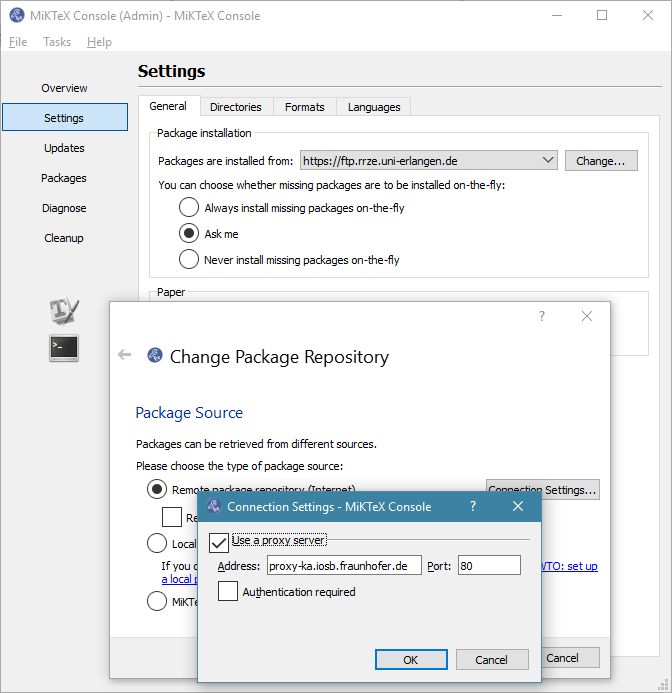
\includegraphics[width=\linewidth]{images/examples/MiKTeX-Proxy.png}%
\caption{MiKTeX-Einstellungen zum Nachladen der Zusatzpakete}%
\label{fig:MiKTeX-Proxy}%
\end{figure}

Nach der MiKTeX-Installation sollte man im Startmenü gleich die MiKTeX-Console aufrufen, den Proxy eintragen und das Update durchführen um die aktuellste Version der vorinstallierten Pakete zu erhalten.
So vermeidet man beim automatischen Nachladen weiterer \glspl{gls:pkg} aus dem \acrshort{ac:CTAN}-Repository etwaige Inkompatibilitäten aufgrund veralteter Stammpakete.


%%%%%%%%%%%%%%%%%%%%%%%%%%%%%%%%%%%%%%%%%%%%%%%%%%%%%%%%%%%%
\subsection{TeXLive-Einstellungen}
\label{sec:TeXLive}
%%%%%%%%%%%%%%%%%%%%%%%%%%%%%%%%%%%%%%%%%%%%%%%%%%%%%%%%%%%%
Bei Verwendung von TeXLive unter Linux muss darauf geachtet werden, dass alle notwendigen Linux-\glspl{gls:pkg} installiert sind.
Unter Ubuntu 17.04 sollte es funktionieren, wenn folgende Linux-\glspl{gls:pkg} installiert wurden:
\begin{itemize*}
	\item {\small\verb#texlive#}
	\item {\small\verb#texlive-lang-german#}
	\item {\small\verb#texlive-fonts-extra#}
	\item {\small\verb#texlive-bibtex-extra#}
	\item {\small\verb#fonts-linuxlibertine#}
	\item {\small\verb#biber#}
	\item {\small\verb#xindy#}
	\item {\small\verb#texmaker#}
\end{itemize*}
Texmaker ist eine IDE für \LaTeX, die aber vermutlich über Dependencies schon einige Pakete mitbringt.


%%%%%%%%%%%%%%%%%%%%%%%%%%%%%%%%%%%%%%%%%%%%%%%%%%%%%%%%%%%%
\subsection{Kompilieraufrufe}
\label{sec:Aufruf}
%%%%%%%%%%%%%%%%%%%%%%%%%%%%%%%%%%%%%%%%%%%%%%%%%%%%%%%%%%%%
Zur erfolgreichen Kompilierung des Dokumentes müssen mehrere
Kommandozeilenprogramme aufgerufen werden.
Bei Verwendung einer integrierten Entwicklungsumgebung (IDE),
wird diese so konfiguriert, dass die Aufrufe aus der IDE heraus erfolgen und
die etwaigen Warnungen, Erfolgs- und Fehlermeldungen in der IDE sichtbar werden.
Die entsprechenden Einstellungen für TeXnicCenter und TeXstudio finden sich
in den nachfolgenden Kapiteln.

Die einzelnen Aufrufe sind:
\begin{itemize*}
\item \index{xelatex}\texttt{xelatex} zur eigentlichen Kompilierung von \LaTeX-Quelltext,
\item \index{biber}\texttt{biber} zur Kompilierung von Bibliografien,
\item \index{makeglossaries}\texttt{makeglossaries}, welches intern \index{xindy}\texttt{xindy} aufruft,
zur Erstellung einer Zwischenausgabe für das Abkürzungsverzeichnis und das Glossar
\index{makexindex}\texttt{makeindex}, welches durch die Verwendung des Pakets \pkg{imakeidx} implizit aufgerufen wird, zur Erstellung des Stichwortverzeichnisses
\end{itemize*}
Bei einem Durchlauf von \texttt{xelatex}, \texttt{biber}, \texttt{makeglossaries} und \texttt{makeindex}
werden die einzelnen Inhalte sowie die entsprechenden Querverweise
zuerst jeweils in eine oder mehrere Zwischendateien hinausgeschrieben,
die sodann wieder eingelesen und verarbeitet werden müssen.
Manche Inhalte werden daher erst jeweils beim zweiten Aufruf von \texttt{xelatex} generiert.
Für die korrekte Generierung eines Dokumentes mit allen Verzeichnissen
(Inhalts-, Abbildungs-, Tabellen-, Literatur, Abkürzungs-, Begriffs und Stichwortverzeichnis),
PDF"=Lesezeichen und korrekt gesetzten Querverweisen,
muss \texttt{xelatex} daher mehrmals aufgerufen werden.

Sollte man ausnahmsweise das Dokument doch noch aus der Kommandozeile oder von einem Script heraus aufrufen wollen,
so ist die Reihenfolge der Aufrufe wie folgt:
\begin{verbatim}
#> xelatex -synctex=1 -interaction=nonstopmode Diss.tex
#> xelatex -synctex=1 -interaction=nonstopmode Diss.tex
#> biber Diss
#> makeglossaries Diss
#> xelatex -synctex=1 -interaction=nonstopmode Diss.tex
#> xelatex -synctex=1 -interaction=nonstopmode Diss.tex
\end{verbatim}

Wenn kein \index{Kompilierfehler}Kompilierfehler aufgetreten ist,
sollte nach dem vierten Durchlauf von \texttt{xelatex} die
\index{Warnung!Please re-run latex}Warnung \enquote{Please re-run latex}
verschwunden sein.
%%%%%%%%%%%%%%%%%%%%%%%%%%%%%%%%%%%%%%%%%%%%%%%%%%%%%%%%%%%%
\section{Aufbau der Vorlage}%
\label{sec:AufbauDerVorlage}
%%%%%%%%%%%%%%%%%%%%%%%%%%%%%%%%%%%%%%%%%%%%%%%%%%%%%%%%%%%%
%
Die Vorlage besteht aus mehreren Dateien und Verzeichnissen.
Ihre Bedeutung ist in \cref{tab:StrukturDerVorlage} zusammengefasst.
%
%{\footnotesize
\begin{table}[htbp]
%\scriptsize% kleinere Schrift
\footnotesize% kleinere Schrift
\centering%% Tabelle zentrieren (falls nicht volle Seitenbreite)
\renewcommand{\arraystretch}{1.5}% Abstand zwischen den Zeilen auf 1,5faches
\setlength{\tabcolsep}{0pt}% Seitliche Abstände eliminieren
% Tabelle auf die Seitenbreite strecken
\begin{tabularx}{\columnwidth}%
% Breite der ersten Spalte auf Inhalt anpassen,
% Breite der zweiten Spalte automatisch bestimmen,
%Spacing zwischen den Spalten auf 10pt setzen:
{l@{\extracolsep{8pt}}X}%
%-----------------------------------------------------------------------------------------------------
\toprule%
%-----------------------------------------------------------------------------------------------------
\bfseries Datei/Verzeichnis               & \bfseries Bedeutung und Benutzerinteraktion\\
%-----------------------------------------------------------------------------------------------------
\midrule%
%-----------------------------------------------------------------------------------------------------
\texttt{./Diss.tcp}                       & TeXnicCenter-Projektdatei. Aufruf im TeXnicCenter.
                                          Indirekte Änderung durch Einstellungen im Programm.\\
%-----------------------------------------------------------------------------------------------------
\texttt{./Diss.tex}                       & \texttt{TeX}-Hauptdatei. Aus- und Einblenden der einzelnen Manuskript-Teile
                                          durch Ersetzen von \lc{showif} durch \lc{hideif} und vice versa.\\
%-----------------------------------------------------------------------------------------------------
\texttt{./bib/Diss.bib}                   & Literaturdatenbank im \texttt{BibLaTeX}-Format. Verwendete Referenzen einfügen.\\
%-----------------------------------------------------------------------------------------------------
\texttt{./content/*}                      & Inhalte der Arbeit. Hier Inhalte der einzelnen \texttt{LaTeX}-Kapitel einfügen.\\
%-----------------------------------------------------------------------------------------------------
\texttt{./figures-src/*}                  & \texttt{TikZ}-Zeichnungen. %(Quellcode).
                                          Ggf. weitere hinzufügen.\\
%-----------------------------------------------------------------------------------------------------
\texttt{./figures-compiled/*}             & Temporäre Kompilate der \texttt{TikZ}-Zeichnungen.
                                          Bei Aktualisierung der \texttt{TikZ}-Zeichnungen löschen.\\
%-----------------------------------------------------------------------------------------------------
\texttt{./fonts/*}                        & Verwendete Schriften. Keine.\\
%-----------------------------------------------------------------------------------------------------
\texttt{./images/*}                       & Bilder im Binärformat. %(jpg, png, pdf etc).
                                          Ggf. weitere hinzufügen. \\
%-----------------------------------------------------------------------------------------------------
\texttt{./preambel/*}                     & Konfigurationsdateien. S.u.\\
%-----------------------------------------------------------------------------------------------------
\texttt{./preambel/Acronyms.tex}          & Definition der Akronyme.
                                          Ggf. weitere hinzufügen.\\
%-----------------------------------------------------------------------------------------------------
\texttt{./preambel/AlleAngaben.tex}       & Angaben zum Typ der Arbeit, zum Autor und zu den Gutachtern.
                                          Einstellung der Hauptsprache.\\
%-----------------------------------------------------------------------------------------------------
\texttt{./preambel/AllePfade.tex}         & Definition von Suchpfaden für Bildverzeichnisse und Bibliografie"=Dateien.
                                          Ggf. ergänzen.\\
%-----------------------------------------------------------------------------------------------------
%\texttt{./preambel/BibSettings.tex}       & Konfiguration der Bibliografie
%                                          Normalerweise keine, es sei denn man möchte den Stil der Literaturverzeichnisse ändern. \\
%-----------------------------------------------------------------------------------------------------
%\texttt{./preambel/EncodingAndFont.tex}   & Schriftarteinstellungen
%                                          Keine.\\
%-----------------------------------------------------------------------------------------------------
\texttt{./preambel/Glossary.tex}          & Definition der Glossar-Einträge.
                                          Ggf. weitere hinzufügen.\\
%-----------------------------------------------------------------------------------------------------
\texttt{./preambel/GlossarySymbols.tex}   & Glossar-Einträge für automatisches Symbolverzeichnis.
                                          Bei Verwendung ergänzen.\\
%-----------------------------------------------------------------------------------------------------
\texttt{./preambel/Header.tex}            & Alle Präambel-Definitionen (\teilw in weiteren Dateien).
                                          Aktivierung der \printkeyword{draft}-Option und des A4-Layouts.\\
%-----------------------------------------------------------------------------------------------------
\texttt{./preambel/Hyphenation.tex}       & Silbentrennung für unbekannte Wörter.
                                          Ggf. Regeln für die Silbentrennung weiterer Begriffe hinzufügen.\\
%-----------------------------------------------------------------------------------------------------
%\texttt{./preambel/IndexStyle.tex}        & Layout des Stichwortverzeichnisses.
%                                          Keine.\\
%-----------------------------------------------------------------------------------------------------
%\texttt{./preambel/KomaOptions.tex}       & KomaScript-Optionen.
%                                          Keine.\\
%-----------------------------------------------------------------------------------------------------
\texttt{./preambel/Math.tex}              & Mathe-Einstellungen und Makros.
                                          Bei Bedarf eigene Mathe-Makros definieren.\\
%-----------------------------------------------------------------------------------------------------
\texttt{./preambel/MyPackages.tex}        & Zusatzpakete
                                          Ggf. Einbindung von Zusatzpaketen.\\
%-----------------------------------------------------------------------------------------------------
\texttt{./preambel/Newcommands.tex}       & Eigene \LaTeX{}-Makros.
                                          Ggf. weitere Makros hinzufügen.\\
%-----------------------------------------------------------------------------------------------------
%\texttt{./preambel/preambel-commands.tex} & Paketkonfigurationen.
%                                          Normalerweise keine.\\
%-----------------------------------------------------------------------------------------------------
%\texttt{./preambel/settings.tex}          & Einstellungen zu Längen, Breiten, Verzeichnistiefen etc.
%                                          Normalerweise keine.\\
%-----------------------------------------------------------------------------------------------------
%\texttt{./preambel/TableCommands.tex}     & Tabelleneinstellungen.
%                                          Normalerweise keine.\\
%-----------------------------------------------------------------------------------------------------
%\texttt{./preamble/Translations.tex}      & Multilinguale Begriffsdefinitionen.
%                                          Normalerweise keine.\\
%-----------------------------------------------------------------------------------------------------
\bottomrule%
%-----------------------------------------------------------------------------------------------------
\end{tabularx}%
\caption[Dateien und Verzeichnisse der Vorlage]{Dateien und Verzeichnisse der Vorlage}%
\label{tab:StrukturDerVorlage}%
\end{table}

Bei der Datei \printfilepath{Diss.tcp} handelt es sich um die Projektdatei für den \LaTeX-Editor TeXnicCenter.
In ihr werden die projektbezogenen Einstellungen des TeXnicCenter festgehalten.
Das sind u.a. Angaben zur Hauptdatei des Projektes und zur Projektsprache.
Die korrekte Angabe der Projektsprache ist insofern wichtig, als dass diese in TeXnicCenter ab Version 2.0 Beta 1 zur Bestimmung der Sprache für die Rechtschreibprüfung verwendet wird.
Die entsprechenden Einstellungen können im TeXnicCenter über den Menüeintrag \printkeyword{Projekt} $\rightarrow$ \printkeyword{Eigenschaften} vorgenommen werden.


Die Hauptdatei ist die Datei \printfilepath{Diss.tex}.
Sie ist verhältnismäßig kurz, da die Hauptinhalte in andere Dateien ausgelagert sind, welche mit Hilfe des \lc{input\{\}} \bzw des \lc{include\{\}}-Befehls eingebunden werden.
Die Hauptdatei besteht im Wesentlichen aus vier Abschnitten.
Im ersten stehen die sogenannten \enquote{Magic comments}, mit deren Hilfe manche \LaTeX-IDEs sich selbst vorkonfigurieren können.
Sie fangen mit \enquote{\texttt{\%~!TeX}} an und geben an, welche Kodierung für die Dateien verwendet wird und welche Programme für die Kompilierung des Quelltextes und der Bibliografie verwendet werden sollen.
Außerdem kann hier angegeben werden, welche Sprache für die Rechtschreibprüfung innerhalb der IDE verwendet werden soll.
Im zweiten Abschnitt wird die Header-Datei eingebunden.
In dieser wird die verwendeten Dokumentklasse (inklusive Papierformat und Schriftgröße) definiert, sowie weitere Dateien eingebunden,
in welchen die zu landenden Pakete, Layout"=Parameter sowie alle weiteren Einstellungen definiert und konfiguriert werden.
Im dritten Teil können mit Hilfe von Schaltern einzelne Teile der Arbeit aus- und wieder eingeblendet werden, ohne dass sie auskommentiert werden müssen.
Im vierten Teil werden nun die einzelnen Inhalte der Arbeit eingebunden.

Das entstehende PDF heißt genauso wie die Hauptdatei.

Die einzelnen \index{Kapitel}Kapiteln der Arbeit werden im Verzeichnis \printfilepath{./content/} als separate Dateien gespeichert.
Es empfiehlt sich als Dateiname das Schema \printfilepath{nn-name.tex} zu verwenden, wobei \printkeyword{nn} die Nummer des Kapitels ist,
sodass die Dateien in der semantisch richtigen Reihenfolge sortiert angezeigt werden.
Die einzelnen Dateien werden per \verb+include{}+-Direktive in der Datei \printfilepath{Diss.tex} eingebunden.
Theoretisch wäre es an dieser Stelle auch möglich mit \verb+\input{}+ zu arbeiten, was jedoch seine Nachteile hätte.
Der Unterschied zwischen den beiden Befehlen wird \href{https://texwelt.de/wissen/fragen/32/was-ist-der-unterschied-zwischen-include-and-input}{auf texwelt.de} erklärt:

\begin{quote}
{\small
\verb+\input{file}+ lädt die Datei an Ort und Stelle in die Ziel-Datei und ist äquivalent
als ob man den Text in \printkeyword{file} direkt in die Ziel-Datei geschrieben hätte.
\verb+\input+ kann letztlich überall für jede Art Datei verwendet werden und kann auch verschachtelt angewendet werden,
d.h. eine eingebundene Datei kann ihrerseits Dateien mit \verb+\input+ einbinden.

\verb+\include{file}+ hingegen führt zunächst einmal ein \verb+\clearpage+ aus bevor es \verb+\input{file}+ ausführt.
Im Gegensatz zu \verb+\input+ kann eine Datei, die mit \verb+\include+ eingebunden wird,
kein weiteres \verb+\include+ enthalten, es ist also keine verschachtelte Anwendung möglich.
Eine mit \verb+\include+ eingebundene Datei kann aber natürlich \verb+\input+ enthalten.
\verb+\include+ erzeugt eine neue \printfilepath{aux}-Datei für die eingebundene Datei.
Das erlaubt es beispielsweise, ein Dokument in mehrere logische Einheiten zu zerlegen (etwa einzelne Kapitel),
die jede einer Datei entsprechen, die mit \verb+\include+ in die Hauptdatei eingebunden wird.
\verb+\includeonly{file1,file3}+ würde dann erlauben, nur gerade bearbeitete Dateien für die Kompilation einzubinden
und durch die separaten \printfilepath{aux}-Dateien dennoch korrekte Seitenzahlen und Querverweise zu erhalten.
Es gibt auch das \pkg{excludeonly} Paket, dessen Befehl \verb+\excludeonly+ das gegensätzliche Verhalten bietet.%
}%
\footnote{\url{https://texwelt.de/wissen/fragen/32/was-ist-der-unterschied-zwischen-include-and-input}}
\end{quote}

Zur besseren Übersicht und zur Vereinfachung der Fehlersuche wird empfohlen,
die einzelnen Unterkapitel ebenfalls als separate Dateien in Unterverzeichnissen von \printfilepath{./content/} anzulegen
und sie mit den \verb+\input{}+-Direktiven in die jeweiligen Kapitel-Dateien einzubinden.

Es wird davon ausgegangen, dass sich sämtliche Bibliografie-Angaben in der Datei
\printfilepath{./bib/Diss.bib} befinden.
Sollten mehrere Bibliografie-Dateien verwendet werden, können diese in der Datei
\printfilepath{./preamble/AllePfade.tex} gesetzt werden.

\index{Bild}Bilder bzw. \index{Zeichnung|see{Bild}}Zeichnungen werden auf zwei Arten eingebunden.
Bilder im \index{Bild!Binär-}Binärformat (PNG, JPEG, TIFF, PDF, etc.)
werden mit \lc{includegraphics}-Befehl eingebunden. 
Bei den \index{Bild!TikZ}\gls{gls:tikz}-Zeichnungen handelt es sich um reguläre TeX-Quellcode-Dateien,
die mit dem \verb+\input+-Befehl eingebunden werden.
Für eine einfache Verwaltung wird empfohlen, Binärbilder im Verzeichnis \printfilepath{./images/} abzulegen.
Zusätzliche Pfade können in der Datei \printfilepath{./preambel/AllePfade.tex} definiert werden.
Die \gls{gls:tikz}-Quellcode-Dateien sollten im Verzeichnis \printfilepath{./figures-src/} abgelegt werden.
Während des Kompilierens werden für jede \gls{gls:tikz}-Zeichnung im Verzeichnis \printfilepath{./figures-compiled/} mehrere Dateien erzeugt.
Der Inhalt dieses Verzeichnisses kann gefahrlos gelöscht werden.
Weitere Hinweise und Beispiele zur Einbindung von Grafiken finden sich in \cref{sec:Bilder}.

Die wichtigsten Einstellungen, die auf jeden Fall geändert werden müssen,
finden sich in der Datei \printfilepath{./preambel/AlleAngaben.tex}.
Hier werden \ua Angaben zum Verfasser, Art und Titel der Arbeit sowie zu den Gutachtern gemacht.
Außerdem wird hier die Hauptsprache der Arbeit gesetzt, was sich an mehreren Stellen auswirkt.
So wird beispielsweise bei Umstellung auf Englisch als Hauptsprache
\enquote{Danksagung} durch \enquote{Acknowledgments},
\enquote{Inhaltsverzeichnis} durch \enquote{Contents}
\usw ersetzt.
Auch die Regeln der Silbentrennung werden entsprechend angepasst.

Regeln zur Silbentrennung unbekannter Wörtern (\zB von Fachbegriffen)
können in der Datei \printfilepath{./preambel/Hyphenation.tex} festgelegt werden.
Zu beachten ist, dass zusammengesetzte Wörter mit einem Bindestrich
ausschließlich am Bindestrich getrennt werden,
wogegen auch ein Eintrag in die Datei \printfilepath{Hyphenation.tex} nicht hilft.
Um Silbentrennung an anderen Stellen eines zusammengesetzten Wortes zu erlauben,
muss man den Bindestrich durch „\verb+"=+“ ersetzen%
\footnote{\url{https://de.wikibooks.org/wiki/LaTeX-W%C3%B6rterbuch:_Silbentrennung}}.

%%%%%%%%%%%%%%%%%%%%%%%%%%%%%%%%%%%%%%%%%%%%%%%%%%%%%%%%%%%%
\section[Grundsätzliches]{Grundsätzliches}%
\label{sec:Grundsätzliches}
%%%%%%%%%%%%%%%%%%%%%%%%%%%%%%%%%%%%%%%%%%%%%%%%%%%%%%%%%%%%
%
Beim Erstellen neuer Dateien bzw. Öffnen und Speichern bereits vorhandener Dateien ist darauf zu achten,
dass stets \index{UTF8-Kodierung}UTF-8 als Zeichenkodierung verwendet wird.
Wichtig ist dabei, dass alle tex-Dateien die UTF8-Kodierung ohne BOM haben,
worauf beim Anlegen neuer TeX-Dateien besonders zu achten ist
(am besten man kopiert und bearbeitet eine bereits vorhandene Datei).

Dank geeigneter Einstellungen in den Header-Dateien können deutsche Umlaute wie 
\index{Umlaute}%
ä,ö,ü,ß, Zeichen mit Akzent wie é sowie weitere UTF8-Zeichen wie z.B.
\index{Anführungszeichen}%
\index{Sprache!unterschiedliche Anführungszeichen}%
„deutsche“, “englische”, »französische« oder «russische» Anführungszeichen 
direkt im Quellcode eingegeben werden ohne irgendwelche Umwege wie z.B. 
\verb+"a+ für ä,
\verb+"u+ für ü,
\verb+\ss+, für ß und
\verb+'e+ für é.
Dies gilt insbesondere auch für Quellen des Literaturverzeichnisses (Bib-Dateien).

Die Zeiten, in welchen man sich bei der Eingabe deutscher Buchstaben verkünsteln musste,
sind zum Glück endgültig vorbei.

\myexcl{Wichtig!}
Normale, gerade Anführungszeichen (\texttt{{\dq}}) haben eine Sonderfunktion und sollten im Quellcode (außer in Listings) nicht verwendet werden.
Für die Eingabe von Anführungszeichen sollte man am besten die entsprechende Textstelle mit dem \lc{enquote\{...\}}"=Befehl umschließen.
Damit werden je nach Spracheinstellung des Dokumentes automatisch die richtigen Anführungszeichen gesetzt.
Außerdem werden so auch die \enquote{verschachtelten \enquote{Anführungszeichen}} korrekt behandelt.

Es empfiehlt sich, die einzelnen Sätze jeweils in einer neuen Zeile anzufangen.
Ein einfaches Zeilenumbruch wird von LaTeX wie ein Leerzeichen gehandhabt
und hat somit keinen Einfluss auf die Zeilenumbrüche im Ergebnisdokument.
Beim Rückwärtsspringen aus der PDF-Datei zum Quellcode wird dadurch jedoch
eine wesentlich bessere Lokalisierung der betroffenen Textstelle ermöglicht.
%%%%%%%%%%%%%%%%%%%%%%%%%%%%%%%%%%%%%%%%%%%%%%%%%%%%%%%%%%%%
\section[% Kurzversion für das Inhaltsverz., Kolumnentitel und PDF-Lesezeichen:
         Wichtiges zu Umbrüchen bei Überschriften
         \mbox{(Kurzversion für das Inhaltsverzeichnis etc.)}%
				]{% Langversion, die im Text gedruckt wird:
         Wichtiges zu Umbrüchen bei Überschriften
         (und ein Beispiel \newline für eine lange Überschrift,
         welche \newline für das Inhaltsverzeichnis und 
         \newline die Kolumnentiteln zu lang ist).%
				}%
\index{Zeilenumbruch}\index{Titel}\index{Überschrift}\index{PDF!Lesezeichen}%
\label{chap:Titles}
%%%%%%%%%%%%%%%%%%%%%%%%%%%%%%%%%%%%%%%%%%%%%%%%%%%%%%%%%%%%
%
%
Bei den Kapitelüberschriften kann man zwei Versionen definieren:
eine lange Überschrift in geschweiften Klammern, welche in der Arbeit selbst angezeigt wird, 
und optional eine Kurzversion in eckigen Klammern, welche im Inhaltsverzeichnis und in den 
\href{https://de.wikipedia.org/wiki/Kolumnentitel}{Kolumnentiteln}%
\footnote{Kolumnentitel sind Überschriften der einzelnen Seiten. Meist stehen sie in der Kopfzeile.}
angezeigt wird:
\begin{latex}
\section[Kurzversion]{Langer Titel}
\end{latex}
Dasselbe gilt für Bild- und Tabellenunterschriften. Hier kann man dem
\lc{caption}-Befehl ebenfalls einen optionalen Parameter übergeben.

Manchmal sind dem \glsdat{ac:KSP} die von \LaTeX{} automatisch eingefügten Zeilenumbrüche in den Kapitelüberschriften im Inhaltsverzeichnis nicht \enquote{schön} genug.
Ein manuelles Einfügen der Zeilenumbrüche etwa mit \verb+\newline+ in der Kurzversion des Titels funktioniert leider nicht,
da diese dann nicht nur im Inhaltsverzeichnis, sondern auch in den Kolumnentiteln und PDF"=Lesezeichen zur Geltung kommen, 
was normalerweise nicht erwünscht ist.

Abhilfe schafft der folgende Trick:
man schließt den letzten, umzubrechenden Teil der Kurzversion des Titels in eine \verb+\mbox{}+.
Der Text, der in eine \verb+\mbox{}+ eingeschlossen wird, darf nicht umbrochen werden.
Im Kolumnentiteln und in den PDF"=Lesezeichen hat dies keine besondere Wirkung; im Inhaltsverzeichnis führt dies jedoch dazu, dass \LaTeX{} den Zeilenumbruch vor der \verb+\mbox{}+ einfügt.
Dasselbe gilt für die ungünstig umbrochene Wörter (so will 
Ein entsprechendes Beispiel stellt die Überschrift dieses Abschnitts dar.
%%%%%%%%%%%%%%%%%%%%%%%%%%%%%%%%%%%%%%%%%%%%%%%%%%%%%%%%%%%%
\section[Bilder, Grafiken und Diagramme]{Bilder, Grafiken und Diagramme}
\label{sec:Bilder}
%%%%%%%%%%%%%%%%%%%%%%%%%%%%%%%%%%%%%%%%%%%%%%%%%%%%%%%%%%%%
%
Bei Einbindung von Grafiken sind zwei Fälle zu unterscheiden:
\begin{itemize*}
  \item reguläre \index{Bild!Binär-}Bilder in einem Binärformat
	      (\texttt{PNG}, \texttt{TIFF}, \texttt{JPG}, \texttt{PDF}, etc.)
	\item \index{Bild!Vektor-}Grafiken, die im \gls{gls:tikz}-Quellcode vorliegen 
\end{itemize*}

Grundlegender Unterschied bei der Einbindung \enquote{regulärer} Bilder
und \gls{gls:tikz}-Bilder ist, dass Binärformatgrafiken mit \lc{includegraphics\{...\}}
eingebunden werden, während \gls{gls:tikz}-Grafiken mit \lc{input\{...\}} eingebunden
und von \texttt{latex} mitkompiliert werden.


%%%%%%%%%%%%%%%%%%%%%%%%%%%%%%%%%%%%%%%%%%%%%%%%%%%%%%%%%%%%
\subsection[Floats]{\index{Float}\index{Bild!Float}Floats}%
\label{sec:Floats}
%%%%%%%%%%%%%%%%%%%%%%%%%%%%%%%%%%%%%%%%%%%%%%%%%%%%%%%%%%%%
%
Üblicherweise werden Bilder und Tabellen in Fließumgebungen (floats) gesetzt,
damit \LaTeX\ sie geschickt positionieren kann.
Bei Bildern heißt die entsprechende Float-Umgebung \printkeyword{figure}.
Die Positionierung kann durch Angabe von Buchstaben
\printkeyword{h}, \printkeyword{t}, \printkeyword{b} und \printkeyword{p}
beeinflusst werden
(\enquote{here}, \enquote{top}, \enquote{bottom}, \enquote{extra page}).

\myexcl{Wichtig!}
Seitens des \glsgen{ac:KSP} wird bezüglich Einbindung von Floats gefordert,
dass diese die einzelnen Sätze nicht zerreißen.
Dies bedeutet, dass eine Platzierung von Bildern und Tabellen lediglich
zwischen zwei Absätzen in Frage kommt.
Allerdings kann es passieren, dass der Platz auf der Seite nicht mehr ausreicht,
und das Bild nicht an der gewünschten Stelle gesetzt werden kann.
Damit wird das Bild auf die nächste Seite verschoben.
Bei aktivierter \printkeyword{t}- oder \printkeyword{b}-Option würde \LaTeX{} versuchen,
das Bild am oberen oder unteren Rand der Seite zu platzieren.
Allerdings passiert das dann häufig mitten in einem Satz,
was vom \gls{ac:KSP} ausdrücklich nicht erwünscht ist.
Somit bleibt eigentlich nur noch die Verwendung der \printkeyword{h}-Option.

Leider können dabei einige unerwünschte Effekte auftreten.
So können beispielsweise auf der vorherigen Seite riesige leere Flächen entstehen.
Wenn der verbleibende Platz auf der Seite eine Platzierung nicht erlaubt,
kann es schnell passieren, dass \LaTeX{} das betroffene Bild 
und alle Folgeilder ans Ende des Kapitels verschiebt
(genauer gesagt, an die Stelle, wo die nächste \lc{clearpage}-Anweisung kommt).

Eine genaue Auswirkung der Parameter
\printkeyword{h}, \printkeyword{t}, \printkeyword{b} und \printkeyword{p}
auf die Bildplatzierung ist nicht immer intuitiv.
Um diese zu verstehen, empfiehlt sich die Lektüre der Beschreibung
von Frank Mittelbach
\href{https://tex.stackexchange.com/questions/39017/how-to-influence-the-position-of-float-environments-like-figure-and-table-in-lat/39020#39020}{auf stackexchange.com}.%
\footnote{\url{https://tex.stackexchange.com/questions/39017/how-to-influence-the-position-of-float-environments-like-figure-and-table-in-lat/39020#39020}}

Prinzipiell empfiehlt sich eine endgültige Platzierung der Bilder erst ganz am Schluss,
nachdem alle anderen Korrekturen durchgeführt sind.
Ggf. müssen die Bilderdefinitionen manuell im Quellcode herumgeschoben werden,
bis die Abbildungen von \LaTeX\ optimal gesetzt werden.
Dafür empfiehlt es sich, die einzelnen Bilddefinitionen in Extra-Dateien auszulagern,
so dass nur noch eine einzige Zeile herumgeschoben werden muss.

%%%%%%%%%%%%%%%%%%%%%%%%%%%%%%%%%%%%%%%%%%%%%%%%%%%%%%%%%%%%
\subsection[Binärbilder]{\index{Bild!Binär-}Binärbilder}%
\label{sec:Binaerbilder}
%%%%%%%%%%%%%%%%%%%%%%%%%%%%%%%%%%%%%%%%%%%%%%%%%%%%%%%%%%%%
%
Ein Beispiel für die Einbindung eines Bildes im Binärformat ist in \cref{lst:binary-image} angeführt:

\begin{latex}[caption={Einbindung einer Binärgrafik in LaTeX},label={lst:binary-image}]
\begin{figure}[h]%
  \centering%
  \includegraphics[width=\linewidth]{Bildpfad/Dateiname}%
  \caption[Kurzversion für das Abbildungsverzeichnis]{%
           Eine tolle sehr lange Abbildungsunterschrift}%
  \label{fig:my-binary-image}%
\end{figure}
\end{latex}

Die Angabe des Pfades kann sowohl absolut als auch relativ
zum Verzeichnis der Hauptdatei oder zu einem der Pfade angegeben werden,
die in der Datei \printfilepath{./preambel/AllePfade.tex} definiert sind.
Diese Pfade werden in angegebenen Reihenfolge durchsucht.
Dasselbe gilt für die Dateierweiterung.
Ist keine Erweiterung definiert und liegen mehrere Bilder mit gleichem Namen jedoch unterschiedlicher Dateierweiterung vor,
wird die Reihenfolge, die in der Datei texttt{AllePfade.tex} definiert ist, verwendet.

Zu beachten ist dabei, dass der \gls{ac:KSP} Skalierung der Bildern auf die Seitenbreite fordert,
was hier durch die Option \printkeyword{width=\bs linewidth} verwirklicht wurde.

Wichtig anzumerken ist, dass alle Zeilen innerhalb der \printkeyword{Figure}"=Umgebung
mit einem Prozentzeichen abzuschließen sind.
Ansonsten werden überflüssige Leerzeichen eingefügt,
was zu unerwünschten Nebenwirkungen führen kann.

Mit Hilfe von Paket \pkg{subfig} \cite{Cochran2005} können Bilder auch in
\index{Abbildung|see{Bild}}\index{Bild!Unterabbildung}Unterabbildungen gesetzt
und sowohl als ganzes (vgl. \cref{fig:subfloat-example}) als auch einzeln (vgl.
\cref{fig:subfloat-example-01,fig:subfloat-example-02,fig:subfloat-example-03,fig:subfloat-example-04})
referenziert werden.

\begin{figure}[h]%
	\centering%
	\subfloat[La Savoureuse, Lepuix, Frankreich (\copyright\ Thomas Bresson)]{%
		\label{fig:subfloat-example-01}%
		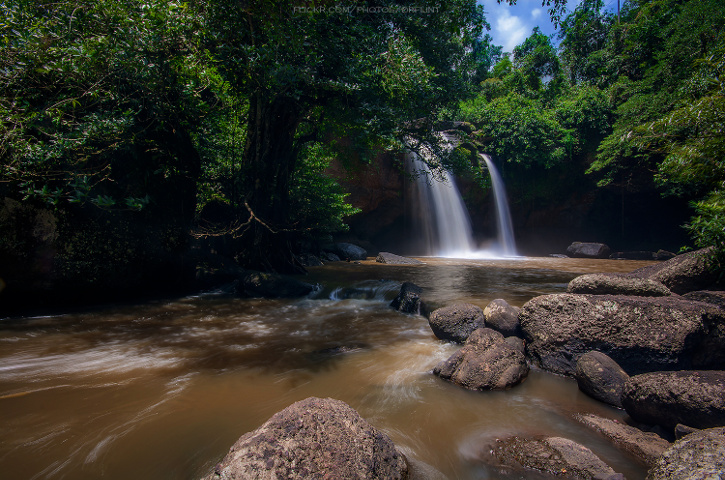
\includegraphics[width=0.49\linewidth]{./images/examples/subfloat-example-01.jpg}%
	}%
	\hfill%
	\subfloat[Bangkok, Thailand (\copyright\ Prachanart Viriyaraks)]{%
		\label{fig:subfloat-example-02}%
		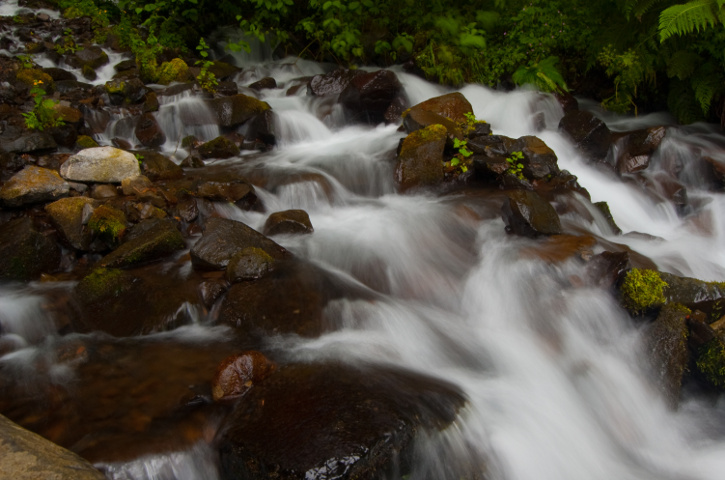
\includegraphics[width=0.49\linewidth]{./images/examples/subfloat-example-02.jpg}%
	}%
	\\%
	\subfloat[Wahkeena Falls, Lincoln Park, USA (\copyright\ srslyguys)]{%
		\label{fig:subfloat-example-03}%
		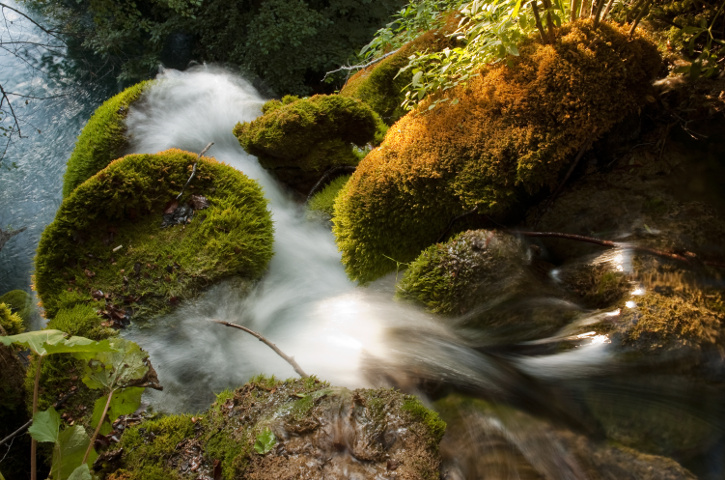
\includegraphics[width=0.49\linewidth]{./images/examples/subfloat-example-03.jpg}%
	}%
	\hfill%
	\subfloat[Nacionalni park Plitvička jezer, Kroatien (\copyright\ Roman Bonnefoy)]{%
		\label{fig:subfloat-example-04}%
		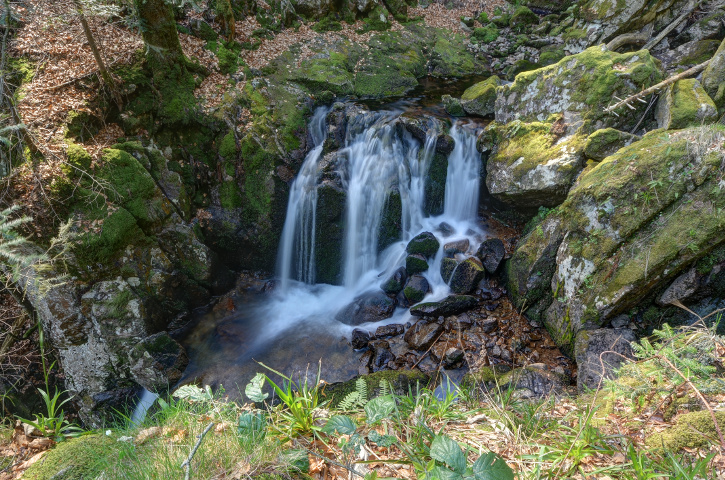
\includegraphics[width=0.49\linewidth]{./images/examples/subfloat-example-04.jpg}%
	}%
	\caption[Bild mit Unterabbildungen]{Wasserfälle der Welt als Beispiel für Unterabbildungen}%
	\label{fig:subfloat-example}%
\end{figure}

Der Beispielcode dafür ist in \cref{lst:subfigures} dargestellt.

\begin{latex}[caption={Unterabbildungen in LaTeX},label={lst:subfigures}]
\begin{figure}[h]%
	\centering%
	\subfloat[Unterbezeichnung 1)]{%
		\label{fig:UnterAbb1}%
		\includegraphics[width=0.49\linewidth]{Bildpfad/Bild1}%
	}%
	\hfill%
	\subfloat[Unterbezeichnung 2]{%
		\label{fig:UnterAbb2}%
		\includegraphics[width=0.49\linewidth]{Bildpfad/Bild2}%
	}%
	\\%
	\subfloat[Unterbezeichnung 3)]{%
		\label{fig:UnterAbb3}%
		\includegraphics[width=0.49\linewidth]{Bildpfad/Bild3}%
	}%
	\hfill%
	\subfloat[Unterbezeichnung 4]{%
		\label{UnterAbb4}%
		\includegraphics[width=0.49\linewidth]{Bildpfad/Bild4}%
	}%
\caption[Kurzversion]{Langversion der Bildunterschrift}%
\label{fig:MeinGanzesBild}%
\end{figure}
\end{latex}

Man beachte die abschließenden Prozent-Zeichen am Ende jeder Zeile!

%%%%%%%%%%%%%%%%%%%%%%%%%%%%%%%%%%%%%%%%%%%%%%%%%%%%%%%%%%%%
\subsection[TikZ-Grafiken]{\index{TikZ}\index{Bild!TikZ}\gls{gls:tikz}-Grafiken}%
\label{sec:TikZ}
%%%%%%%%%%%%%%%%%%%%%%%%%%%%%%%%%%%%%%%%%%%%%%%%%%%%%%%%%%%%
%
\Gls{gls:tikz} eignet sich hervorragend, um wissenschaftliche Zeichnungen,
Vektorgrafiken und \index{Diagramm}Diagramme direkt mithilfe von LaTeX
zu setzen, sodass die Schrift direkt zum restlichen Dokument passt.
Zu dem \pkg{tikz}-\gls{gls:pkg} und dem darauf aufsetzenden \pkg{PGFplots}-\gls{gls:pkg} gibt
es hervorragende Dokumentation \parencites{Tantau2013}{Feuersaenger2014}.
Mit \gls{gls:tikz} und \gls{gls:pgfplots} lassen sich viele gute Sachen machen.


Der Code für die Einbindung einer \gls{gls:tikz}-Grafik sieht folgendermaßen aus:
\begin{latex}[caption={Einbindung einer TikZ-Zeichnung in LaTeX},label={lst:tikz-figure}]
\begin{figure}[h]%
  \centering%
  \tikzsetnextfilename{TikZ-Bild}%
  \resizebox{\textwidth}{!}{%   <--- optionale Skalierung
    \input{./figures-src/TikZ-Bild.tex}%
  }%                            <--- optionale Skalierung
  \caption[Kurzversion für das Abbildungsverzeichnis]{%
           Eine tolle sehr lange Abbildungsunterschrift}%
  \label{fig:my-tikz-figure}%
\end{figure}
\end{latex}

Eine Skalierung auf die volle Seitenbreite oder ein vielfaches davon im Falle von Unterabbildungen kann bei Bedarf mit Hilfe der Anweisung
\texttt{\bs resizebox\{\bs textwidth\}\{!\}\{...\}}
durchgeführt werden.

Das Kommando \verb+\tikzsetnextfilename{...}+ ist nicht unbedingt notwendig,
 aber sehr zu empfehlen, da dies als Name für das temporäre Kompilat im Ordner
\printfilepath{./figures-compiled/} genommen wird.
Dieser sollte gleich dem Namen des Quelldatei (ohne Endung) gewählt werden.
Ansonsten nimmt \texttt{pdflatex} eine hochlaufende Nummer als Dateiname,
was die Fehlersuche sehr erschwert.

Nachfolgend finden sich einige Beispiele für TikZ-Zeichnungen, nämlich
eine Übersicht über die KIT-Corporate-Identity-Farben (\cref{fig:kit-colors}),
ein kommutatives Diagramm (\cref{fig:kpca}),
ein Netzwerkkommunikationsgraph (\cref{fig:net-comm}),
einfache \index{Diagramm!Punkt-}Punktdiagramme (\cref{fig:ica})
und etwas aufwendigere Diagramme mit mehreren
\index{Achsensystem|see{Diagramm}}Achsensystemen (\cref{fig:pca}).

Vorzugsweise sollten für die Grafiken die KIT-Corporate-Identity-Farben verwendet werden,
die sowohl eine RGB"=Definition für die Darstellung online,
als auch eine CMYK"=Definition für den Offset-Druck haben.%
\footnote{Bei Erstellung der Manuskriptversionen
für die Online-Veröffentlichung bzw. für den Offset-Druck
ist auf die korrekte Einstellung der Option \printkeyword{useCMYKcolors}
in der Datei \printfilepath{preambel/AlleAngaben.tex} zu achten
(\printkeyword{false} für die Online-Veröffentlichung und \printkeyword{true} für den Druck!}

\begin{figure}[hp]%
	\centering%
  \tikzsetnextfilename{kit-colors}%
	%\resizebox{\textwidth}{!}{%
		\begin{tikzpicture}[
box/.append style={rectangle,inner sep=0pt,outer sep=0pt,minimum size=1.5em,draw=none,fill=#1},
label/.style={font={\ttfamily\footnotesize},anchor=east},
caption/.style={font={\ttfamily\footnotesize},rotate=90,anchor=west}
]
\matrix[row sep=.2em,column sep=.2em] {
  &
\node[caption] {\textbackslash{}KITgreen...};      &
\node[caption] {\textbackslash{}KITblue...};       &
\node[caption] {\textbackslash{}KITblack...};      &
\node[caption] {\textbackslash{}KITpalegreen...};  &
\node[caption] {\textbackslash{}KITyellow...};     &
\node[caption] {\textbackslash{}KITorange...};     &
\node[caption] {\textbackslash{}KITbrown...};      &
\node[caption] {\textbackslash{}KITred...};        &
\node[caption] {\textbackslash{}KITlilac...};      &
\node[caption] {\textbackslash{}KITcyanblue...};   \\
\node[label] {};               &
\node[box=KITgreen      ] {};  &
\node[box=KITblue       ] {};  &
\node[box=KITblack      ] {};  &
\node[box=KITpalegreen  ] {};  &
\node[box=KITyellow     ] {};  &
\node[box=KITorange     ] {};  &
\node[box=KITbrown      ] {};  &
\node[box=KITred        ] {};  &
\node[box=KITlilac      ] {};  &
\node[box=KITcyanblue   ] {};  \\
\node[label] {...70};      &
\node[box=KITgreen70    ] {};  &
\node[box=KITblue70     ] {};  &
\node[box=KITblack70    ] {};  &
\node[box=KITpalegreen70] {};  &
\node[box=KITyellow70   ] {};  &
\node[box=KITorange70   ] {};  &
\node[box=KITbrown70    ] {};  &
\node[box=KITred70      ] {};  &
\node[box=KITlilac70    ] {};  &
\node[box=KITcyanblue70 ] {};  \\
\node[label] {...50};      &
\node[box=KITgreen50    ] {};  &
\node[box=KITblue50     ] {};  &
\node[box=KITblack50    ] {};  &
\node[box=KITpalegreen50] {};  &
\node[box=KITyellow50   ] {};  &
\node[box=KITorange50   ] {};  &
\node[box=KITbrown50    ] {};  &
\node[box=KITred50      ] {};  &
\node[box=KITlilac50    ] {};  &
\node[box=KITcyanblue50 ] {};  \\
\node[label] {...30};      &
\node[box=KITgreen30    ] {};  &
\node[box=KITblue30     ] {};  &
\node[box=KITblack30    ] {};  &
\node[box=KITpalegreen30] {};  &
\node[box=KITyellow30   ] {};  &
\node[box=KITorange30   ] {};  &
\node[box=KITbrown30    ] {};  &
\node[box=KITred30      ] {};  &
\node[box=KITlilac30    ] {};  &
\node[box=KITcyanblue30 ] {};  \\
\node[label] {...15};      &
\node[box=KITgreen15    ] {};  &
\node[box=KITblue15     ] {};  &
\node[box=KITblack15    ] {};  &
\node[box=KITpalegreen15] {};  &
\node[box=KITyellow15   ] {};  &
\node[box=KITorange15   ] {};  &
\node[box=KITbrown15    ] {};  &
\node[box=KITred15      ] {};  &
\node[box=KITlilac15    ] {};  &
\node[box=KITcyanblue15 ] {};  \\
};

\end{tikzpicture}%
	%}%
	\caption{KIT-Corporate-Identity-Farben}%
  \label{fig:kit-colors}%
\end{figure}

\begin{figure}[hp]%
	\centering%
  \tikzsetnextfilename{kpca}%
	%\resizebox{\textwidth}{!}{%
		\begin{tikzpicture}
\node (M) at (0,0) {$M$};
\node (F) [right=5em of M] {$F$};
\node (N) [right=5em of F] {$M'$};

\draw[-latex] (M)--(F) node[above,midway,font=\scriptsize] {$\varphi$};
\draw[-latex] (F)--(N) node[above,midway,font=\scriptsize] {PCA};
\draw[-latex,dotted] (M) to[bend left] node[above,midway,font=\scriptsize] {kernelized PCA} (N);

\node[below=3ex of M,font=\scriptsize] {$\dim(M) = d$};
\node[below=3ex of F,font=\scriptsize] {$\dim(F) \gg d$};
\node[below=3ex of N,font=\scriptsize] {$\dim(M') = d' < d$};
\end{tikzpicture}%
	%}%
	\caption{Kommutative Diagramm mit TikZ}%
  \label{fig:kpca}%
\end{figure}

\begin{figure}[hp]%
	\centering
  \tikzsetnextfilename{net-comm}%
	\resizebox{\textwidth}{!}{%
		\begin{tikzpicture}[
every node/.append style={font={\sffamily}},
caption/.append style={font={\sffamily\bfseries}},
comm/.style={-latex,semithick},
msg/.style={midway,sloped,above,font={\sffamily\small}},
]
\matrix[row sep=3ex,column sep=25mm] {
\node[caption] {Partner 1};  & \node[caption] {Partner 2}; & \node[caption] {Partner 3}; \\
\node (A1) {Aktion 1}; & & \\
& \node (A2) {Aktion 2}; & \\
\node (A3) {Aktion 3}; & & \\
& & \node (A4) {Aktion 4};\\
& \node (A5) {Aktion 5}; & \\
\node (A6) {Aktion 6}; & & \\
};

\draw[comm] (A1)--(A2) node[msg] {Nachricht 1};
\draw[comm] (A2)--(A3) node[msg] {Nachricht 2};
\draw[comm] (A3)--(A4) node[msg] {Nachricht 3};
\draw[comm] (A4)--(A5) node[msg] {Nachricht 4};
\draw[comm] (A5)--(A6) node[msg] {Nachricht 5};

\end{tikzpicture}%
	}%
	\caption{Netzwerkkommunikationsgraph mit TikZ}%
  \label{fig:net-comm}%
\end{figure}

\begin{figure}[hp]%
	\centering%
	\subfloat[Ursprünglicher Merkmalsraum]{%
		\label{fig:ica-1}%
		\tikzsetnextfilename{ica-1}%
		\resizebox{0.45\textwidth}{!}{%
			\begin{tikzpicture}[
my_plot/.style={draw=none,every mark/.append style={draw=KITblue,fill=KITblue},mark=*,mark size=1.5pt},
]

\begin{axis}[
width=4cm,
height=4cm,
xmin = -1.1,
xmax = 1.1,
xlabel={$m_1$},
ymin = -1.1,
ymax = 1.1,
ylabel={$m_2$},
axis lines=center,
scale only axis,
]

\addplot[my_plot] coordinates {
(0.030,-0.062) (-0.118,-0.004) (0.276,0.236) (0.578,0.566) (-0.143,-0.014)
(0.304,0.257) (0.423,0.535) (0.205,0.344) (0.364,0.365) (-0.327,-0.368)
(0.176,0.310) (-0.298,-0.360) (0.153,0.279) (0.010,0.062) (0.150,0.231)
(-0.301,-0.214) (0.079,0.094) (-0.241,-0.161) (-0.474,-0.461) (0.091,0.173)
(0.541,0.601) (-0.288,-0.153) (0.013,-0.093) (0.290,0.115) (0.194,0.028)
(0.486,0.370) (0.201,0.227) (0.510,0.510) (-0.211,-0.293) (-0.058,0.088)
(0.326,0.176) (-0.591,-0.574) (0.071,0.204) (-0.401,-0.308) (0.206,0.111)
(-0.529,-0.667) (0.064,0.040) (0.032,0.035) (-0.349,-0.291) (0.476,0.316)
(0.625,0.624) (0.312,0.234) (0.076,-0.079) (0.016,0.018) (-0.556,-0.655)
(-0.308,-0.217) (0.248,0.122) (-0.515,-0.428) (-0.121,0.041) (0.260,0.228)
(-0.317,-0.406) (0.650,0.483) (-0.198,-0.097) (-0.427,-0.495) (0.429,0.553)
(-0.432,-0.538) (-0.460,-0.440) (-0.558,-0.654) (0.516,0.586) (-0.230,-0.205)
(0.148,0.199) (-0.417,-0.240) (-0.138,-0.040) (-0.252,-0.403) (0.096,0.010)
(-0.478,-0.339) (0.628,0.650) (0.054,-0.104) (0.502,0.429) (0.051,0.045)
(0.099,0.106) (0.344,0.214) (-0.359,-0.334) (0.291,0.187) (0.176,0.217)
(0.329,0.362) (-0.270,-0.116) (-0.136,-0.008) (-0.446,-0.533) (0.653,0.585)
(0.474,0.540) (0.093,0.136) (0.356,0.473) (0.232,0.217) (0.592,0.659)
(-0.326,-0.170) (-0.683,-0.497) (-0.484,-0.357) (-0.607,-0.635) (-0.044,-0.041)
(-0.681,-0.533) (-0.306,-0.401) (0.189,0.334) (0.420,0.259) (0.040,0.086)
(-0.148,-0.303) (-0.585,-0.507) (0.424,0.330) (0.597,0.688) (0.211,0.271)
(-0.429,-0.360) (0.280,0.188) (0.375,0.252) (-0.505,-0.528) (-0.064,-0.043)
(-0.257,-0.140) (0.302,0.262) (-0.228,-0.293) (0.154,0.122) (-0.549,-0.403)
(0.034,-0.027) (0.207,0.122) (-0.538,-0.648) (-0.601,-0.664) (-0.623,-0.433)
(-0.552,-0.417) (-0.094,-0.166) (0.469,0.496) (0.580,0.497) (0.212,0.159)
(0.515,0.627) (-0.070,-0.167) (-0.101,-0.015) (-0.244,-0.328) (-0.372,-0.477)
(0.256,0.199) (-0.607,-0.560) (-0.462,-0.554) (0.132,0.086) (0.066,0.050)
(0.230,0.157) (-0.502,-0.556) (0.666,0.490) (0.407,0.425) (-0.219,-0.355)
(-0.250,-0.285) (0.266,0.159) (-0.263,-0.412) (0.028,0.091) (-0.086,0.043)
(-0.633,-0.504) (-0.420,-0.399) (0.378,0.380) (-0.008,-0.163) (-0.226,-0.278)
(0.148,0.193) (-0.629,-0.582) (0.586,0.450) (0.025,0.136) (-0.445,-0.360)
};

\end{axis}
\end{tikzpicture}
		}%
	}%
	\hfill%
	\subfloat[Transienter Merkmalsraum (Nach Whitening, z.\,B. durch \gls{ac:PCA} inkl. Normalisierung)]{%
		\label{fig:ica-2}%
		\tikzsetnextfilename{ica-2}%
		\resizebox{0.45\textwidth}{!}{%
			\begin{tikzpicture}[
my_plot/.style={draw=none,every mark/.append style={draw=KITblue,fill=KITblue},mark=*,mark size=1.5pt},
]

\begin{axis}[
width=4cm,
height=4cm,
xmin = -1.1,
xmax = 1.1,
xlabel={$m'_1$},
ymin = -1.1,
ymax = 1.1,
ylabel={$m'_2$},
axis lines=center,
scale only axis,
]

\addplot[my_plot] coordinates {
(-0.273,-0.278) (0.267,0.398) (0.117,-0.289) (0.483,-0.399) (0.293,0.455)
(0.120,-0.326) (0.747,0.049) (0.640,0.265) (0.329,-0.231) (-0.430,0.090)
(0.597,0.269) (-0.471,0.014) (0.549,0.259) (0.180,0.141) (0.401,0.136)
(0.014,0.439) (0.120,-0.008) (0.044,0.379) (-0.384,0.338) (0.349,0.173)
(0.681,-0.175) (0.183,0.566) (-0.335,-0.309) (-0.310,-0.678) (-0.368,-0.593)
(0.057,-0.637) (0.266,-0.054) (0.457,-0.325) (-0.457,-0.098) (0.425,0.450)
(-0.196,-0.631) (-0.474,0.426) (0.500,0.334) (-0.059,0.516) (-0.127,-0.402)
(-0.926,-0.054) (-0.019,-0.107) (0.038,-0.012) (-0.122,0.388) (-0.094,-0.754)
(0.560,-0.398) (0.026,-0.418) (-0.439,-0.488) (0.021,-0.004) (-0.822,0.075)
(0.020,0.454) (-0.190,-0.516) (-0.180,0.573) (0.420,0.535) (0.130,-0.255)
(-0.575,-0.050) (0.039,-0.885) (0.151,0.410) (-0.607,0.078) (0.790,0.077)
(-0.736,-0.026) (-0.348,0.349) (-0.817,0.082) (0.692,-0.130) (-0.126,0.216)
(0.301,0.052) (0.202,0.765) (0.195,0.363) (-0.719,-0.267) (-0.195,-0.306)
(0.024,0.696) (0.635,-0.338) (-0.469,-0.483) (0.215,-0.523) (0.028,-0.048)
(0.113,-0.042) (-0.116,-0.587) (-0.242,0.298) (-0.078,-0.479) (0.291,0.003)
(0.405,-0.114) (0.259,0.605) (0.297,0.450) (-0.684,0.038) (0.365,-0.607)
(0.644,-0.112) (0.223,0.062) (0.701,0.104) (0.158,-0.192) (0.752,-0.185)
(0.214,0.646) (-0.007,0.960) (-0.020,0.667) (-0.635,0.308) (-0.029,0.037)
(-0.131,0.849) (-0.587,-0.076) (0.645,0.292) (-0.150,-0.724) (0.184,0.102)
(-0.638,-0.344) (-0.270,0.594) (0.073,-0.536) (0.833,-0.122) (0.385,0.036)
(-0.160,0.468) (-0.048,-0.437) (-0.065,-0.586) (-0.531,0.254) (0.010,0.099)
(0.151,0.495) (0.141,-0.305) (-0.417,-0.039) (0.033,-0.188) (-0.016,0.763)
(-0.166,-0.191) (-0.093,-0.373) (-0.843,0.031) (-0.746,0.204) (0.060,0.933)
(-0.055,0.733) (-0.320,-0.144) (0.510,-0.221) (0.252,-0.601) (0.018,-0.283)
(0.829,-0.011) (-0.381,-0.230) (0.190,0.308) (-0.492,-0.081) (-0.679,-0.062)
(0.042,-0.326) (-0.391,0.520) (-0.717,0.032) (-0.032,-0.214) (0.009,-0.085)
(-0.034,-0.355) (-0.627,0.168) (0.022,-0.923) (0.424,-0.209) (-0.641,-0.245)
(-0.339,0.060) (-0.110,-0.472) (-0.722,-0.253) (0.230,0.160) (0.345,0.421)
(-0.147,0.768) (-0.309,0.326) (0.348,-0.233) (-0.513,-0.434) (-0.372,-0.002)
(0.278,0.031) (-0.413,0.531) (0.082,-0.757) (0.384,0.297) (-0.122,0.523)
};

\end{axis}
\end{tikzpicture}%
		}%
	}%
	\hfill%
	\subfloat[Transformierter Merkmalsraum]{%
		\label{fig:ica-3}%
		\tikzsetnextfilename{ica-3}%
		\resizebox{0.45\textwidth}{!}{%
			\begin{tikzpicture}[
my_plot/.style={draw=none,every mark/.append style={draw=KITblue,fill=KITblue},mark=*,mark size=1.5pt},
]

\begin{axis}[
width=4cm,
height=4cm,
xmin = -1.1,
xmax = 1.1,
xlabel={$m''_1$},
ymin = -1.1,
ymax = 1.1,
ylabel={$m''_2$},
axis lines=center,
scale only axis,
]

\addplot[my_plot] coordinates {
(-0.389,-0.004) (0.470,0.093) (-0.122,-0.287) (0.059,-0.623) (0.529,0.115)
(-0.146,-0.316) (0.563,-0.493) (0.640,-0.265) (0.069,-0.396) (-0.241,0.367)
(0.613,-0.232) (-0.323,0.342) (0.572,-0.205) (0.227,-0.027) (0.379,-0.188)
(0.320,0.300) (0.079,-0.090) (0.299,0.237) (-0.033,0.510) (0.369,-0.124)
(0.358,-0.605) (0.530,0.271) (-0.455,0.019) (-0.699,-0.260) (-0.680,-0.159)
(-0.410,-0.491) (0.150,-0.226) (0.093,-0.554) (-0.393,0.254) (0.619,0.017)
(-0.584,-0.307) (-0.034,0.636) (0.590,-0.118) (0.323,0.406) (-0.374,-0.194)
(-0.693,0.617) (-0.089,-0.062) (0.018,-0.035) (0.188,0.361) (-0.600,-0.467)
(0.114,-0.678) (-0.277,-0.314) (-0.655,-0.035) (0.012,-0.018) (-0.528,0.634)
(0.335,0.306) (-0.499,-0.230) (0.278,0.532) (0.676,0.081) (-0.088,-0.272)
(-0.442,0.371) (-0.599,-0.654) (0.397,0.183) (-0.374,0.484) (0.613,-0.504)
(-0.539,0.502) (0.001,0.493) (-0.520,0.635) (0.398,-0.581) (0.063,0.242)
(0.249,-0.176) (0.684,0.398) (0.395,0.119) (-0.697,0.320) (-0.354,-0.078)
(0.509,0.475) (0.210,-0.688) (-0.674,-0.010) (-0.218,-0.522) (-0.014,-0.053)
(0.050,-0.110) (-0.498,-0.333) (0.040,0.382) (-0.394,-0.284) (0.208,-0.204)
(0.206,-0.367) (0.611,0.245) (0.528,0.108) (-0.457,0.510) (-0.171,-0.688)
(0.376,-0.535) (0.202,-0.114) (0.569,-0.422) (-0.024,-0.247) (0.401,-0.663)
(0.608,0.305) (0.674,0.684) (0.457,0.486) (-0.231,0.667) (0.005,0.047)
(0.508,0.693) (-0.469,0.362) (0.663,-0.250) (-0.618,-0.406) (0.203,-0.058)
(-0.694,0.208) (0.229,0.611) (-0.327,-0.431) (0.503,-0.676) (0.298,-0.247)
(0.217,0.444) (-0.343,-0.275) (-0.460,-0.368) (-0.196,0.555) (0.077,0.063)
(0.457,0.243) (-0.116,-0.315) (-0.322,0.267) (-0.110,-0.157) (0.528,0.550)
(-0.253,-0.018) (-0.329,-0.198) (-0.574,0.618) (-0.384,0.672) (0.702,0.617)
(0.480,0.557) (-0.329,0.124) (0.205,-0.517) (-0.247,-0.604) (-0.188,-0.213)
(0.578,-0.594) (-0.432,0.106) (0.352,0.083) (-0.406,0.291) (-0.523,0.436)
(-0.201,-0.260) (0.091,0.644) (-0.484,0.530) (-0.173,-0.129) (-0.054,-0.067)
(-0.275,-0.227) (-0.325,0.562) (-0.637,-0.668) (0.152,-0.447) (-0.626,0.280)
(-0.197,0.283) (-0.411,-0.256) (-0.690,0.332) (0.276,-0.050) (0.542,0.054)
(0.439,0.647) (0.012,0.449) (0.081,-0.411) (-0.670,0.056) (-0.265,0.262)
(0.218,-0.175) (0.083,0.668) (-0.477,-0.594) (0.482,-0.061) (0.284,0.456)
};

\end{axis}
\end{tikzpicture}%
		}%
}%
\caption{Diagramme mit TikZ direkt in LaTeX (hier: Die Schritte der \enquote{Independent component analysis})}%
\label{fig:ica}%
\end{figure}

\begin{figure}[hp]
	\centering%
	\subfloat[Ungünstige Projektion]{%
		\label{fig:pca-1}%
		\tikzsetnextfilename{pca-1}%
		\resizebox{0.48\textwidth}{!}{%
			\begin{tikzpicture}[
my_plot_1/.style={draw=none,every mark/.append style={draw=KITblue,fill=KITblue},mark=*},
my_plot_2/.style={draw=none,every mark/.append style={draw=KITred,fill=KITred},mark=*},
trans_arrow/.style={semithick,KITorange,-latex},
]

\begin{axis}[
width=4cm,
height=4cm,
xmin = -0.2,
xmax = 2.3,
xlabel={$m_1$},
ymin = -0.2,
ymax = 2.3,
ylabel={$m_2$},
xticklabel=\empty,
yticklabel=\empty,
axis lines=center,
clip=false,
scale only axis,
]

\addplot[my_plot_1] coordinates {
(1.3,0.38)
(1.42,0.71)
(1.48,0.60)
(1.64,0.54)
(1.65,0.81)
(1.68,0.89)
(1.79,1.11)
(1.88,1.18)
(1.89,1.46)
(1.94,1.35)
(1.86,1.65)
(2.02,1.83)
(2.12,1.83)
(2.19,2.26)
(2.21,2.07)
};

\addplot[my_plot_2] coordinates {
(1.28,0.58)
(1.33,0.93)
(1.54,1.03)
(1.54,1.26)
(1.51,1.41)
(1.72,1.52)
(1.76,1.87)
(1.80,1.90)
(1.90,2.00)
(1.91,2.27)
(2.05,2.40)
};

\coordinate(CoM) at (axis cs:1.71,1.38) {};

\draw[trans_arrow] (axis cs:0,0)--(CoM) node[midway,above left] {$m_0$};

\end{axis}

\begin{axis}[
width=5cm,
height=2.5cm,
xmin = -1.5,
xmax = 1.5,
xlabel={$m'_1$},
ymin = -0.75,
ymax = 0.75,
ylabel={$m'_2$},
axis lines=center,
xlabel style={anchor=north west},
ylabel style={anchor=south west},
xticklabel=\empty,
yticklabel=\empty,
clip=false,
anchor=origin,
at={(CoM)},
rotate around={65:(current axis.origin)},
clip=false,
scale only axis
]

\addplot+[my_plot_1] coordinates {
(-2,-0.0510)
(-2,-0.0203)
(-2,-0.1212)
(-2,-0.2916)
(-2,-0.1865)
(-2,-0.1799)
(-2,-0.1866)
(-2,-0.2386)
(-2,-0.1293)
(-2,-0.2211)
(-2,-0.0218)
(-2,-0.0908)
(-2,-0.1814)
(-2,-0.0631)
(-2,-0.1615)
};

\addplot+[my_plot_2] coordinates {
(-2,0.0516)
(-2,0.1542)
(-2,0.0062)
(-2,0.1034)
(-2,0.1939)
(-2,0.0501)
(-2,0.1618)
(-2,0.1382)
(-2,0.0898)
(-2,0.1949)
(-2,0.1229)
};

\draw[trans_arrow,shorten <=2pt,shorten >=3pt] (axis cs:-1.5,0)--(axis cs:-2,0) node[midway,right,font={\footnotesize},align=left] {Projektion\\auf $e_2$};
\draw[semithick] (axis cs:-2,-0.5)--(axis cs:-2,0.4);

\addplot+[my_plot_1] coordinates {
(-1.0796,-1.5)
(-0.7298,-1.5)
(-0.8041,-1.5)
(-0.7909,-1.5)
(-0.5420,-1.5)
(-0.4568,-1.5)
(-0.2109,-1.5)
(-0.1094,-1.5)
(0.1486,-1.5)
(0.0700,-1.5)
(0.3081,-1.5)
(0.5389,-1.5)
(0.5811,-1.5)
(1.0004,-1.5)
(0.8367,-1.5)
};

\addplot+[my_plot_2] coordinates {
(-0.9068,-1.5)
(-0.5684,-1.5)
(-0.3891,-1.5)
(-0.1806,-1.5)
(-0.0573,-1.5)
(0.1311,-1.5)
(0.4652,-1.5)
(0.5093,-1.5)
(0.6422,-1.5)
(0.8911,-1.5)
(1.0681,-1.5)
};

\draw[trans_arrow,shorten <=2pt,shorten >=3pt] (axis cs:0,-0.75)--(axis cs:0,-1.5) node[midway,anchor=north east,font={\footnotesize},align=left] {Projektion\\auf $e_1$};
\draw[semithick] (axis cs:-1.3,-1.5)--(axis cs:1.3,-1.5);

\end{axis}

\end{tikzpicture}%
		}%
	}\hfill%
	\subfloat[Zielführende Projektion]{%
		\label{fig:pca-2}%
		\tikzsetnextfilename{pca-2}%
		\resizebox{0.48\textwidth}{!}{%
			\begin{tikzpicture}[
my_plot_1/.style={draw=none,every mark/.append style={draw=KITblue,fill=KITblue},mark=*},
my_plot_2/.style={draw=none,every mark/.append style={draw=KITred,fill=KITred},mark=*},
trans_arrow/.style={semithick,KITorange,-latex},
]

\begin{axis}[
width=4cm,
height=4cm,
xmin = -0.2,
xmax = 2.3,
xlabel={$m_1$},
ymin = -0.2,
ymax = 2.3,
ylabel={$m_2$},
xticklabel=\empty,
yticklabel=\empty,
axis lines=center,
clip=false,
scale only axis,
]

\addplot[my_plot_1] coordinates {
(1.3,0.38)
(1.28,0.58)
(1.42,0.71)
(1.48,0.60)
(1.64,0.54)
(1.33,0.93)
(1.65,0.81)
(1.68,0.89)
(1.54,1.03)
(1.54,1.26)
(1.79,1.11)
(1.88,1.18)
(1.51,1.41)
};

\addplot[my_plot_2] coordinates {
(1.72,1.52)
(1.89,1.46)
(1.94,1.35)
(1.86,1.65)
(1.76,1.87)
(1.80,1.90)
(1.90,2.00)
(2.02,1.83)
(2.12,1.83)
(1.91,2.27)
(2.19,2.26)
(2.21,2.07)
(2.05,2.40)
};

\coordinate(CoM) at (axis cs:1.71,1.38) {};

\draw[trans_arrow] (axis cs:0,0)--(CoM) node[midway,above left] {$m_0$};

\end{axis}

\begin{axis}[
width=5cm,
height=2.5cm,
xmin = -1.5,
xmax = 1.5,
xlabel={$m'_1$},
ymin = -0.75,
ymax = 0.75,
ylabel={$m'_2$},
axis lines=center,
xlabel style={anchor=north west},
ylabel style={anchor=south west},
xticklabel=\empty,
yticklabel=\empty,
clip=false,
anchor=origin,
at={(CoM)},
rotate around={65:(current axis.origin)},
clip=false,
scale only axis
]

\addplot+[my_plot_1] coordinates {
(-2,-0.0510)
(-2,0.0516)
(-2,-0.0203)
(-2,-0.1212)
(-2,-0.2916)
(-2,0.1542)
(-2,-0.1865)
(-2,-0.1799)
(-2,0.0062)
(-2,0.1034)
(-2,-0.1866)
(-2,-0.2386)
(-2,0.1939)
};

\addplot+[my_plot_2] coordinates {
(-2,0.0501)
(-2,-0.1293)
(-2,-0.2211)
(-2,-0.0218)
(-2,0.1618)
(-2,0.1382)
(-2,0.0898)
(-2,-0.0908)
(-2,-0.1814)
(-2,0.1949)
(-2,-0.0631)
(-2,-0.1615)
(-2,0.1229)
};

\draw[trans_arrow,shorten <=2pt,shorten >=3pt] (axis cs:-1.5,0)--(axis cs:-2,0) node[midway,right,font={\footnotesize},align=left] {Projektion\\auf $e_2$};
\draw[semithick] (axis cs:-2,-0.5)--(axis cs:-2,0.4);

\addplot+[my_plot_1] coordinates {
(-1.0796,-1.5)
(-0.9068,-1.5)
(-0.7298,-1.5)
(-0.8041,-1.5)
(-0.7909,-1.5)
(-0.5684,-1.5)
(-0.5420,-1.5)
(-0.4568,-1.5)
(-0.3891,-1.5)
(-0.1806,-1.5)
(-0.2109,-1.5)
(-0.1094,-1.5)
(-0.0573,-1.5)
};

\addplot+[my_plot_2] coordinates {
(0.1311,-1.5)
(0.1486,-1.5)
(0.0700,-1.5)
(0.3081,-1.5)
(0.4652,-1.5)
(0.5093,-1.5)
(0.6422,-1.5)
(0.5389,-1.5)
(0.5811,-1.5)
(0.8911,-1.5)
(1.0004,-1.5)
(0.8367,-1.5)
(1.0681,-1.5)
};

\draw[trans_arrow,shorten <=2pt,shorten >=3pt] (axis cs:0,-0.75)--(axis cs:0,-1.5) node[midway,anchor=north east,font={\footnotesize},align=left] {Projektion\\auf $e_1$};
\draw[semithick] (axis cs:-1.3,-1.5)--(axis cs:1.3,-1.5);

\end{axis}

\end{tikzpicture}%
		}%
	}%
	\caption{Aufwändiges Diagramm mit TikZ (hier: Probleme der \enquote{Principal component analysis})}%
	\label{fig:pca}%
\end{figure}
%%%%%%%%%%%%%%%%%%%%%%%%%%%%%%%%%%%%%%%%%%%%%%%%%%%%%%%%%%%%
\section{Tabellen}%
\label{sec:Tabellen}
%%%%%%%%%%%%%%%%%%%%%%%%%%%%%%%%%%%%%%%%%%%%%%%%%%%%%%%%%%%%
Für eine ausführliche Erläuterung auch über gute und schlechte Tabellen
und deren Gestaltung empfiehlt sich die Lektüre des entsprechenden Artikels im \LaTeX{}"=Kompendium auf Wikibooks%
\footnote{\url{https://de.wikibooks.org/wiki/LaTeX-Kompendium:_Tabellen}}
sowie die Dokumentation des \pkg{booktabs}-Pakets \cite{Fear2005}.
\Ua stellt dieses Paket die Befehle
\begin{itemize*}
	\item \lstinline|\toprule|
	\item \lstinline|\midrule|
	\item \lstinline|\bottomrule|
\end{itemize*}
zur Verfügung.

Eine einfache Tabelle hat den folgenden Code:

\begin{latex}[caption={Einfache Tabelle in \LaTeX},label={lst:tabellenbeispiel}]
\begin{table}%
	\centering%
	\begin{tabularx}{\columnwidth}{l l X}%
		\toprule%
		Datei       &  Bedeutung    &  Benutzerinteraktion \\%
		\midrule%
		Diss.tex  &  Hauptdatei   &  nein     \\%
		images/   &  Bilder       &  ja       \\%
		content/  &  Kapitel      &  ja       \\%
		\bottomrule%
	\end{tabularx}%
	\caption{Dateien der Vorlage}%
	\label{tab:tabellenbeispiel}%
\end{table}
\end{latex}

Das Ergebnis sieht man in \cref{tab:tabellenbeispiel}.

\begin{table}%
	\centering%
	\begin{tabular}{l l l}%
		\toprule%
		Datei       &  Bedeutung    &  Benutzerinteraktion \\%
		\midrule%
		Diss.tex  &  Hauptdatei   &  nein     \\%
		images/   &  Bilder       &  ja       \\%
		content/  &  Kapitel      &  ja       \\%
		\bottomrule%
	\end{tabular}%
	\caption{Dateien der Vorlage}%
	\label{tab:tabellenbeispiel}%
\end{table}

Etwas komplizierter wird es, wenn man eine Tabelle mit alternierender Farbe einfügen möchte (\cref{tab:AlternierendeZeilenfarben}).

\begin{table}
\caption{Tabelle mit alternierender Zeilenfarbe}%
\label{tab:AlternierendeZeilenfarben}%
	\tablestyle%
	\tablealtcolored%
	\begin{tabular}{*{2}{v{0.45\textwidth}}}
		\toprule%
		\tableheadcolor%
		\tableheadformat Tabellenkopf &	\tableheadformat Tabellenkopf
		\tabularnewline%
		\midrule%
		%% Zwischenkopf ---------------------------------------------
		\multicolumn{2}{>{\columncolor{tablesubheadcolor}}l}{\bfseries\color{KITblue} Zwischenkopf}%
		\tabularnewline%
		%%-----------------------------------------------------------
		Inhalt  & Inhalt \tabularnewline
		Inhalt  & Inhalt \tabularnewline
		Inhalt  & Inhalt \tabularnewline
		%% Zwischenkopf ---------------------------------------------
		\multicolumn{2}{>{\columncolor{tablesubheadcolor}}l}{\bfseries\color{KITgreen} Zwischenkopf}%
		\tabularnewline
		%%-----------------------------------------------------------
		Inhalt  & Inhalt \tabularnewline
		Inhalt  & Inhalt \tabularnewline
		\bottomrule%
	\end{tabular}%
\end{table}

%% ------------------------------------------------------------
Lange Tabellen, die umbrochen werden sollen, können mit
\lstinline|\LTXtable{\textwidth}{Datei}|
eingebunden werden, wobei die Tabelle in eine Datei ausgelagert werden muss.
Ein Beispiel dafür sieht man in \cref{tab:MehrseitigeTabelle}.

\IfDefined{LTXtable}{%
	%--Einstellungen für Tabellen ----------
	\colorlet{tablerowcolor}{gray!10.0}%
	\renewcommand\tableheadcolor{\rowcolor{tableheadcolor}}%
	\renewcommand\tablehead{%
			\tableheadfontsize%
			\sffamily\bfseries%
			\slshape%
			\color{black}%
	}%
	%---------------------------------------
	{
		\tablestyle%
		%\tablealtcolored
		\rowcolors{1}{tablerowcolor}{white!100}%
		 \LTXtable{\textwidth}{tables/LongTableExample.tex}%
	}%
} % End If 
%
%
%
Sollten eine Tabelle einmal so breit sein, dass sie nicht mehr horizontal auf
eine Seite passt, so ist es natürlich möglich, diese mithilfe des Pakets
\printkeyword{rotfloat} \parencite{Sommerfeldt2004} in eine
\printkeyword{sidewaystable} statt in eine \printkeyword{table}-Umgebung zu setzen.
Also so:
\begin{latex}[caption={Gedrehte Tabelle},label={lst:rotated-table}]
\begin{sidewaystable}
  \centering%
  \begin{tabular}{...}%
    ...
  \end{tabular}%
  \caption{Bezeichnung}%
  \label{Referenzmarke}%
\end{sidewaystable}%
\end{latex}

Das Ergebnis sieht man in \cref{tab:ex-sideways}.

%% Um 90° gedrehte Tabelle
%
\begin{sidewaystable}[p]
\scriptsize%
%\tiny
\centering%
\begin{tabular}{l M M M M M}%
\toprule%
\addlinespace[0pt]%
 & \multicolumn{5}{c}{\bfseries Level} \tabularnewline
 & \multicolumn{2}{c}{\bfseries Qualitative} & \multicolumn{3}{c}{\bfseries Quantitative} \tabularnewline
 & \bfseries\centering Nominal & \bfseries\centering Ordinal & \bfseries\centering Interval & \bfseries\centering Ratio & \bfseries\centering Absolute \tabularnewline \addlinespace[0pt]\midrule\addlinespace[0pt]
Empirical relation &
\begin{tabitemize}\item[$\sim$] Equivalence\end{tabitemize} &
\begin{tabitemize}\item[$\sim$] Equivalence\item[$\prec$] Ordering\end{tabitemize} &
\begin{tabitemize}\item[$\sim$] Equivalence\item[$\prec$] Ordering\end{tabitemize} &
\begin{tabitemize}\item[$\sim$] Equivalence\item[$\prec$] Ordering\strut\end{tabitemize} &
\begin{tabitemize}\item[$\sim$] Equivalence\item[$\prec$] Ordering\strut\end{tabitemize} \tabularnewline \midrule
Empirical operation &
 &
 &
\begin{tabitemize}\item[$\oplus$] Addition\end{tabitemize} &
\begin{tabitemize}\item[$\oplus$] Addition\item[$\otimes$] Multiplication\strut\end{tabitemize} &
\begin{tabitemize}\item[$\oplus$] Addition\item[$\otimes$] Multiplication\strut\end{tabitemize} \tabularnewline \midrule
Feasable transformation &
$m' = f( m )$ for $f$ bij.\strut &
$m' = f( m )$ for $f$ mon.\strut &
$m' = am + b$ for $a>0$\strut &
$m' = am$ for $a>0$\strut &
$m' = m$\strut \tabularnewline \midrule
Examples of features &
\begin{tabitemize}\item Telephone numbers\item Postal codes\item Gender\strut\end{tabitemize} &
\begin{tabitemize}\item Grades\item Degree of hardness\item Wind intensity\strut\end{tabitemize} &
\begin{tabitemize}\item Temperatur in F\textdegree\item Calendric time\item Geographic altitude\strut\end{tabitemize} &
\begin{tabitemize}\item Temperatur in K\item Mass\item Length\item Electric current\strut\end{tabitemize} &
\begin{tabitemize}\item Quantum numbers\item Error number\strut\end{tabitemize} \tabularnewline \midrule
Range of features &
\begin{tabitemize}\item Numbers\item Names\item Symbols\strut\end{tabitemize} &
Natural numbers &
Real numbers &
Real, positive numbers &
Natural numbers \tabularnewline \midrule
Expressiveness & low & \dots & \dots & \dots & high\strut \tabularnewline \addlinespace[0pt]
\bottomrule%
\end{tabular}%
\caption{Beispiel für eine breite, gedrehte Tabelle (hier: Taxonomie der Maßskalen)}%
\label{tab:ex-sideways}%
\end{sidewaystable}
%%%%%%%%%%%%%%%%%%%%%%%%%%%%%%%%%%%%%%%%%%%%%%%%%%%%%%%%%%%%
\section{Mathematische Sätze, Lemmas, Definitionen etc.}%
\label{sec:Theoreme}
%%%%%%%%%%%%%%%%%%%%%%%%%%%%%%%%%%%%%%%%%%%%%%%%%%%%%%%%%%%%
%
Für eine mathematische Ausarbeitung gibt es LaTeX-\glspl{gls:umgebung}, um
\index{Satz|see{Theorem}}\index{Theorem}Sätze (Theoreme), \index{Lemma|see{Theorem}}Lemma,
\index{Beispiel|see{Theorem}}Beispiele etc. im üblichen Stil von
Mathematik-Büchern zu setzen und zu referenzieren. Vordefiniert sind die
\glspl{gls:umgebung}
\begin{itemize*}
  \item \texttt{theorem} für Sätze
  \item \texttt{definition} für Definitionen
  \item \texttt{lemma} für Lemma
  \item \texttt{corollary} für Korollare
  \item \texttt{proposition} für Propositionen
\end{itemize*}
Die übliche Verwendung ist
\begin{latex}[caption={Beispiel für Theorem-Umgebungen},label={lst:ntheorem}]
\begin{theorem}[Optionaler Name]\label{thm:my-theorem}
...
\end{theorem}
\end{latex}
Weitere Informationen findet man in der Dokumentation zum \texttt{ntheorem}-Paket
\parencite{May2011}. Das Ganze sieht dann beispielsweise wie folgt aus.

\begin{theorem}[Theorem von Arthur Dent]
\label{thm:arthur-dent} Die Antwort auf die Frage nach dem Leben, dem Universum und den ganzen Rest ist 42.
\end{theorem}

\begin{definition}
\LaTeX{} ist eine von Leslie Lamport 1980 entwickelter Satz von Makros zur Erweiterung von \TeX.
\end{definition}

\begin{proposition}[Zweifelhafte Folgerung]
LaTeX ist schön. Beweis folgt unmittelbar aus \cref{thm:arthur-dent}.
\end{proposition}

%%%%%%%%%%%%%%%%%%%%%%%%%%%%%%%%%%%%%%%%%%%%%%%%%%%%%%%%%%%%
\section{Quellcode-Listings}%
\index{Listing!Gestaltungsstil}%
\label{sec:Listings}
%%%%%%%%%%%%%%%%%%%%%%%%%%%%%%%%%%%%%%%%%%%%%%%%%%%%%%%%%%%%
%
Zum Einbinden und formatieren von \index{Code|see{Listing}}Quellcode"=Beispielen
-- sog. \index{Listing}Listings -- wird das Paket \pkg{listings}
\parencite{Hoffmann2014} verwendet.
Das Hervorheben von \index{Schlusselwort@Schlüsselwort}Schlüsselwörtern
wird von LaTeX automatisch erledigt,
wenn die korrekte Sprache des Listings angegeben ist.
Dies geschieht mit Hilfe der Option \printkeyword{language}
oder durch die Angabe eines entsprechend definierten Gestaltungsstils.

Im Befehl \lstinline|\lstset{...}|,
welcher in der Datei \printfilepath{preambel/preambel.tex} zu finden ist,
kann man einen globalen Stil für alle Listings vorgeben
(welcher jedoch bei Bedarf im Einzelfall überrufen werden kann).
Aktuell ist der etwas weiter oben im Code mit dem Befehl
\lstinline|\lstdefinestyle{...}| vordefinierte Stil
\printkeyword{latex} als Standardgestaltungsstil ausgewählt.

Neben \printkeyword{latex} sind in der Datei \printfilepath{preambel/preambel.tex}
auch noch \printkeyword{java} und \printkeyword{C++} als Gestaltungsstile vordefiniert.
Bei Bedarf lassen sich dort weitere Stile definieren und auswählen.

Zur Vereinfachung der Einbindung wurden zusätzlich Umgebungen
\printkeyword{latex}, \printkeyword{java} und \printkeyword{C++}
vordefiniert, die im Code mit \lstinline|\begin{<name>}...\end{<name>}|
direkt verwendet werden können (s. \cref{lst:java-listing}).
%
So bewirkt beispielsweise
%
\begin{latex}[caption={Beispiel eines Listings in Java},label={lst:java-listing}]
\begin{java}[caption={A Java Hello-World example},%
             label={lst:hello-world}]
public class HelloWorld {
  public static void main( String[] args ) {
    System.out.println( "HelloWorld" );
  }
}
\end{java}
\end{latex}
%
das folgende Ergebnis:
%
\begin{C++}[caption={A Java Hello-World example},label={lst:hello-world}]
public class HelloWorld {
  public static void main( String[] args ) {
    System.out.println( "HelloWorld" );
  }
}
\end{C++}

Man beachte, dass anders als bei Abbildungen und Tabellen
die Bezeichnung (\texttt{caption}) und die Referenzmarke (\texttt{label})
nicht als gesonderte Befehle sondern als optionale Argumente übergeben werden.
Dies liegt daran, dass ein Listing in der Regel keine Fließumgebung ist,
sondern an der Stelle im Text erscheint, an der sie im Code auch steht.
Ferner folgt ein Listing den ganz normalen Seitenumbruchsregeln.
Das heißt, überlanger Code wird einfach umgebrochen. 
Um ein Listing zu einem Fließobjekt zu machen, muss das optionale Argument
\texttt{float=<tbp>} angegeben werden.
Die \index{Platzierung}Plazierungsangabe \enquote{\texttt{h}} für \enquote{hier}
ist nicht erlaubt. Denn dies ist das Standardverhalten ohne \texttt{float}.
%%%%%%%%%%%%%%%%%%%%%%%%%%%%%%%%%%%%%%%%%%%%%%%%%%%%%%%%%%%%
\section{Querverweise und Hyperlinks}%
\label{sec:Querverweise}
%%%%%%%%%%%%%%%%%%%%%%%%%%%%%%%%%%%%%%%%%%%%%%%%%%%%%%%%%%%%
%
Querverweise sollten nicht mit dem Befehl \lstinline|\ref{...}| gesetzt werden,
sondern mit \lstinline|\cref{...}| und verwandten Befehlen aus dem Paket
\pkg{cleveref} \cite{Cubitt2013}.
Diese Befehle haben den Vorteil nicht nur die Nummer zu referenzieren,
sondern auch den Typ mit anzugeben.
Hinzu kommt eine intelligente Verwendung der Pluralform und
\index{Sortierung}Sortierung bei Mehrfachaufzählungen auch unterschiedlichen Typs.
Will man \bspw auf zwei Abbildungen und eine Tabelle mit den Marken (\enquote{Labels})
%
\begin{itemize*}
\item \texttt{fig:subfloat-example}
\item \texttt{tab:files-dirs-of-template}
\item \texttt{fig:kit-colors}
\end{itemize*}
%
verweisen, so schreibt man einfach per Komma getrennt
%
\begin{latex}[caption={Cleveres Referenzieren mit \bs cref},label={lst:cref}]
\cref{fig:subfloat-example,
      tab:ex-sideways,
      fig:kit-colors}
\end{latex}
%
und erhält als Resultat
\enquote{\cref{fig:subfloat-example,tab:ex-sideways,fig:kit-colors}}.

\index{URL}\index{Internetadresse|see{URL}}Internetadressen werden in das Kommando \lstinline|\url{...}| eingefasst.
Außerdem besteht die Möglichkeit mit dem Befehl \lstinline|\href{<URL>}{Text}| eine Textstelle mit einem Hyperlink zu versehen.
%%%%%%%%%%%%%%%%%%%%%%%%%%%%%%%%%%%%%%%%%%%%%%%%%%%%%%%%%%%%
\section{Mathematik}%
\label{sec:Mathe}
%%%%%%%%%%%%%%%%%%%%%%%%%%%%%%%%%%%%%%%%%%%%%%%%%%%%%%%%%%%%
%
Grundsätzlich gilt, was in \parencites{ams1999a}{ams1999b} steht. In der Datei
\printfilepath{preambel/05-math.tex} sind eine Menge Kurzkommandos definiert, um eine
einheitliche Typografie von \index{Skalare}Skalaren, \index{Vektoren}Vektoren,
\index{Matrizen}Matrizen, \index{Zufallsvariablen}Zufallsvariablen etc.
zur vereinfachen. In diese Dateien einfach mal reinschauen, welche Kurzkommandos
es gibt.

Auf zwei besondere Kommandos wird näher eingegangen, weil dies häufig falsch
gemacht wird.
\begin{itemize}
  \item Für die Matrixtransponierte gibt es das Kommando \verb#\Tr#, also
	\verb#$A^{\Tr}$# liefert $A^{\Tr}$
	
	\item Bei \index{Integral}Integralen muss das \enquote{Differential-d} gemäß
	ISO in aufrechter Schrift als Operator gesetzt sein mit einem kleinen Abstand
	zum Integranden. Hierfür gibt es das spezielle Kommando \verb#\diff#. Also
	\begin{equation}
	 \int^1_0 x^2 d x = \frac{1}{3} \qquad \text{(falsche Typografie!)}
	\end{equation}
	ist falsch, während \verb#\int^1_0 x^2 \diff x = \frac{1}{3}# das Richtige
	liefert
	\begin{equation}
	 \int^1_0 x^2 \diff x = \frac{1}{3} \qquad \text{(richtige Typografie!)}
	\end{equation}
\end{itemize}

%%%%%%%%%%%%%%%%%%%%%%%%%%%%%%%%%%%%%%%%%%%%%%%%%%%%%%%%%%%%
\section{Abkürzungsverzeichnis, Stichwortverzeichnis (Index) und Glossar}%
\label{sec:Glossare}
%%%%%%%%%%%%%%%%%%%%%%%%%%%%%%%%%%%%%%%%%%%%%%%%%%%%%%%%%%%%
%
Die Vorlage unterstützt auch ein Stichwortverzeichnis und ein Glossar. Ein
Stichwortverzeichnis (oder Index) ist einfach nur eine alphabetisch sortierte
Liste von Begriffen mit einer Auflistung der \index{Fundstelle}Fundstellen
im Dokument. Ein Glossar ist eine alphabetisch sortierte Liste von Begriffen mit
\index{Erklarung@Erklärung}Erklärung.

Der Index wird erzeugt, indem im Quellcode der Befehl \verb#\index{Begriff}#
eingefügt wird. Wichtig, der Begriff selbst wird dadurch nicht gedruckt, sondern
muss noch einmal wiederholt werden, um auch gedruckt zu werden. Dieses Verhalten
ist beabsichtigt, sodass im Index immer nur die Grundform des Wortes verwendet
wird, aber im Text natürlich die richtige Deklination. Also:
\begin{latex}[caption={Beispiel für Index},label={lst:index}]
Die meisten Funktionen dieser \index{Vorlage}Vorlage, werden durch
\index{Paket}Standardpakete bereitgestellt.
\end{latex}
Obiges Beispiel erzeugt einen Indexeintrag für \enquote{Vorlage} der auf
\enquote{Vorlage} verweist und einen Eintrag \enquote{Paket} der auf 
\enquote{Standardpaket} verweist.

Um ein Glossar zu erzeugen, müssen die Glossarbegriffe zunächst definiert werden.
Dies geschieht in der Datei \texttt{./content/00-glossary-definitions.tex}.
Es gibt zwei Haupttypen von Glossarbegriffen: Abkürzungen (Akronyme) und allg.
Einträge (z.\,B. Fachtermini).

Abkürzungen werden mit
\begin{latex}[caption={Definition von Abkürzungen},label={lst:acro}]
\newacronym[%
  shortplural={AUen},%
  longplural={Abgasuntersuchungen}%
] {au}{AU}{Abgasuntersuchung}
\end{latex}
Die drei Hauptargumente sind in dieser Reihenfolge Marke, Abkürzung und
Ausschreibung. Optionale Argumente sind die kurze und lange Pluralform.

Allgemeine Glossarbegriffe werden mit
\begin{latex}[caption={Definition von allg. Glossareinträgen},label={lst:gls}]
\longnewglossaryentry{pkg}{%
  name={Paket},%
  plural={Pakete}}%
{%
  Hier folgt eine lange Definition, die auch mehr als einen
	Absatz beinhalten darf.
}
\end{latex}
erzeugt.

Im Text werden die Einträge durch den Befehl \verb#\gls{gls:Marke}# verwendet.
Der wesentliche Unterschied zwischen einer Abkürzung und einem allg.
Glossareintrag ist, dass bei Abkürzungen bei erstmaliger Verwendung die
Abkürzung gedruckt und die Langform in Klammer dahinter gesetzt wird.
Bei allg. Glossareinträgen wird einfach nur der Name gesetzt. Statt
\verb#\gls{gls:Marke}# gibt es noch viele weitere Befehle, um im Kontext des
umgebenen Textes die korrekte Pluralform, Großschreibung am Satzanfang, etc.
zu gewährleisten. Hierfür konsultiere man das Handbuch zum Paket \texttt{glossaries}
(Pluralform, sic!) \parencite{talbot2014}.

%%%%%%%%%%%%%%%%%%%%%%%%%%%%%%%%%%%%%%%%%%%%%%%%%%%%%%%%%%%%
\section{Randnotizen}%
\label{sec:Randnotizen}
%%%%%%%%%%%%%%%%%%%%%%%%%%%%%%%%%%%%%%%%%%%%%%%%%%%%%%%%%%%%
%
Randnotizen 
\marginnote{Ich bin eine überflüssige Randnotiz}%
werden mit dem Kommando \lc{partitle} gesetzt.
Diese eignet sich zum Beispiel um im Text Stellen zu kennzeichnen,
an denen man noch arbeiten sollte.
Da die Vorgaben des \glsgen{ac:KSP} für den Seitenlayout
einen sehr kleinen Randbereich vorsehen, der zudem nicht bedruckt werden darf,
werden keine Randnotizen in der endgültigen Version des Manuskriptes akzeptiert.
Die Randnotizen lassen sich bequem in der Hauptdatei ausschalten,
indem man \texttt{\bs showif\{showMarginNotes\}}
zu \texttt{\bs hideif\{showMarginNotes\}} ändert.
%%%%%%%%%%%%%%%%%%%%%%%%%%%%%%%%%%%%%%%%%%%%%%%%%%%%%%%%%%%%
\section{Einige DOs und DON'Ts}%
\label{sec:DOsAndDONTs}
%%%%%%%%%%%%%%%%%%%%%%%%%%%%%%%%%%%%%%%%%%%%%%%%%%%%%%%%%%%%

In diesem Kapitel sind einige LaTeX-Dinge zusammengesammelt, die immer wieder
auch von Personen verkehrt gemacht werden, die bereits längere Zeit mit LaTeX
arbeiten. Dies soll hier also keine Einführung in LaTeX werden, sondern spiegelt
nur meine Erfahrung der häufigsten Fehler wieder. Außerdem soll gezeigt werden,
wie bestimmte Dinge innerhalb dieser Vorlage gemacht werden.

Grundsätzlich sollte man bei \index{Problem}Problemen nie, nimmer, niemals einfach nach
einer Lösung im Internet suchen. 95\,\% der Lösungen im Internet sind
bestenfalls falsch, aber eigentlich der größte Mist für den die jeweiligen
Autoren angespitzt in den Boden gerammt, im eigen Saft gegart, gevierteilt und
anschließend in Beton gegossen gehören. Aber eigentlich ist es schade um den
guten Beton.

\subsection{Dokumentationsquellen}

Statt wahllos im Internet nach \index{Losung@Lösung}Lösungen zu suchen, sucht man direkt auf
\url{http://www.ctan.org/tex-archive/} nach dem Paketnamen und verwendet die
dortige Originaldokumentation des Paketautors selbst. Dort zu findende \index{Warnung}Warnungen
sollte man ernst nehmen und nicht machen, auch wenn irgendwo anders behauptet
wird, es würde so funktionieren. Es funktioniert NICHT oder nur scheinbar.

Im Rahmen dieser Vorlage sind insbesondere die \index{Dokumentation}Dokumentationen aus dem
Literaturverzeichnis wärmstens zu empfehlen.

\subsection{Fließumgebungen (Floats)}

Fließumgebungen sind bei LaTeX blockbildende \index{Element!blockbildend}Elemente,
die nicht an der Stelle erscheinen, an der sie im Quellcode definiert sind sondern aus optischen
Gründen an umhergeschoben werden können. Typische Beispiele sind Tabellen,
Bilder, längere Codeausschnitte und ähnliche Dinge. Später wird noch auf
Bilder und Tabellen im Detail eingegangen, aber an diese Stelle sollen vier
Todsünden in Bezug auf Fließumgebungen abgehandelt werden.

Todsünde Nummer eins ist die Verwendung der \index{Platzierung}Platzierungsangabe \texttt{H}, also
bspw.
\begin{latex}[caption={Verbot von \texttt{H} als Platzierungsangabe},label={lst:prohibited-h}]
\begin{figure}[H]
\end{figure}
\end{latex}
um zu erzwingen, dass ein Fließobjekt an dieser Stelle (engl. \enquote{here})
passiert, wenn \texttt{h} nicht genügt. Wenn \texttt{h} nicht genügt, dann liegt
der Fehler bereits woanders und man sollte in das Log schauen, warum LaTeX
die Umgebung nicht platzieren kann und das originäre Problem lösen. Alles andere
macht es nur schlimmer.

Todsünde Nummer zwei ist die Verwendung von Leerzeilen innerhalb der
Fließumgebung oder auch das Abrücken der Fließumgebung mit einer Leerzeile von
dem Text der die Fließumgebung referenziert. Leerzeilen sind bei LaTeX Absätze
und damit potentielle Stellen für Seitenumbrüche. Korrekt ist also folgendes:
\begin{latex}[caption={Verbot von Leerzeilen},label={lst:prohibited-blank-lines}]
Ein Text der auf die \cref{fig:my-fig} verweist
\begin{figure}[h]%
  \centering%
  \includegraphics[width=\linewidth]{Bildpfad/Dateiname}%
  \caption[Kurzversion]{Lange Beschriftung}%
  \label{fig:my-fig}%
\end{figure}
und ohne Leerzeile an der figure-Umgebung dransteht.

Dies ist nun ein neuer Absatz.
\end{latex}
Wie man erkennen kann, steht die \texttt{figure}-Umgebung sogar mitten im Satz
zu der sie gehört. Der häufigste Grund, warum die Platzierungsoptionen
\texttt{t}, \texttt{b}, \texttt{h} und  \texttt{p} nicht so verhalten, wie
man erwartet, ist, dass die \texttt{figure}-Umgebung aus Gründen der Übersicht
mit Leerzeilen abgesetzt wird, sodass diese dann für LaTeX einen eigenen Block
bildet.

Todsünde Nummer drei ist die Verwendung von \verb#\begin{center}# und
\verb#\end{center}# statt von \verb#\centering# innerhalb der Fließumgebung.
Ersteres erzeugt wieder einen internen Absatz und damit einen eigenen Block.
Dies ist also genauso schlimm wie Leerzeilen.

Todsünde Nummer vier ist die falsche Reihenfolge von \verb#\caption{...}# und
\verb#\label{...}#. Die Reihenfolge ist \emph{immer} das Objekt selbst (also
\verb#\includegraphics# oder \verb#tabular#, usw.), dann folgt \verb#\caption{...}#
und zum Schluss \verb#\label{...}#.

\subsection{URLs}

\index{Internetadresse|see{URL}}Internetadressen werden in das Kommando \verb#\url{...}# eingefasst

\subsection{Anführungszeichen}

Um irgendwas in Anführungszeichen einzufassen, wird das Kommando 
\verb#\enquote{...}# verwendet. Dies hat den Vorteil, dass man sich nicht um die
korrekte typografische Variation der Anführungszeichen in Abhängigkeit der
\index{Sprache}Sprache kümmern muss und auch verschachtelte Anführungszeichen korrekt behandelt
werden. Also aus
\begin{latex}[caption={Behandlung von Anführungszeichen},label={lst:quotes},escapechar=\#]
 \enquote{Beim Erreichen der K#ü#ste sprach Hamlet: \enquote{Es ist etwas faul im Staate D#ä#nemark}}.
\end{latex}
wird \enquote{Beim Erreichen der Küste sprach Hamlet: \enquote{Es ist etwas faul
im Staate Dänemark}} mit korrekt verschachtelten einfachen Anführungszeichen.
%%%%%%%%%%%%%%%%%%%%%%%%%%%%%%%%%%%%%%%%%%%%%%%%%%%%%%%%%%%%
\section[Globale Sprachumstellung und temporäre Sprachumschaltung]{Globale Sprachumstellung und temporäre Sprachumschaltung bei fremdsprachlichen Begriffen und Textabschnitten}%
\index{Fremdsprachen}%
\index{Sprache!Fremdsprache}%
\index{Sprache!globale Umstellung}%
\index{Sprache!temporäre Umschaltung}%
\label{sec:Sprache}
%%%%%%%%%%%%%%%%%%%%%%%%%%%%%%%%%%%%%%%%%%%%%%%%%%%%%%%%%%%%
%
Die Hauptsprache der Arbeit wird in der Datei \printfilepath{./preambel/AlleSchalter.tex} festgelegt.
Aktuell werden nur Deutsch und Englisch als Hauptsprachen unterstützt.
Die Auswahl geschieht mit der Angabe des Wertes \printkeyword{true} oder \printkeyword{false}
in der Zeile \lstinline|\setUserDefinedBoolean{englishAsMainLanguage}{<Wert>}|.

Bei Verwendung von fremdsprachlichen Begriffen oder Textabschnitten
(\zB bei englischen oder französischen Zitaten in einer deutschsprachigen Arbeit
oder bei deutschen Begriffen in einer englischsprachigen Arbeit),
sollte man dies entsprechend markieren,
damit \LaTeX{} die richtigen Regeln für die \index{Silbentrennung}Silbentrennung
und die passenden Anführungszeichen bei Verwendung des Befehls
\lstinline|\enquote{...}| ansetzt.
Für die einzelnen Begriffe und kürzere Texte gibt es den Befehl
\lstinline|\foreignlanguage{Sprache}{...}|.
Dann wird für den Text in den geschweiften Klammern die in den eckigen Klammern angegebene Sprache verwendet.
Um die Sprache bis zum nächsten Aufruf des gleichen Kommandos dauerhaft umstellen,
gibt es den Befehl \lstinline|\selectlanguage{Sprache}|.
Es gilt eine Liste der Sprachen aus dem Paket \pkg{babel}.
Für Deustch sollte \printkeyword{ngerman} verwendet werden, was für die
\index{Rechtschreibung!neue deutsche}neue deutsche Rechtschreibung steht.

Für eine korrekte Behandlung der deutschen Kurzfassung und des englischen Abstracts
unabhängig von der gewählten Hauptsprache ist durch die Verwendung der Befehle
\lstinline|\textInGerman{...}| und \lstinline|\textInEnglish{...}| bereits gesorgt.
%
% Alte Anleitung von Philipp Woock
%%%%%%%%%%%%%%%%%%%%%%%%%%%%%%%%%%%%%%%%%%%%%%%%%%%%%%%%%%%%%
\section{Voraussetzungen}%
\label{sec:Voraussetzungen}
%%%%%%%%%%%%%%%%%%%%%%%%%%%%%%%%%%%%%%%%%%%%%%%%%%%%%%%%%%%%

Zunächst eine Liste der technischen Voraussetzungen um diese Vorlage nutzen zu können.

\begin{itemize}
	\item Windows-PC mit \LaTeX-Distribution (Getestet ist Win XP SP3 und Win 7 64-bit jeweils mit MikTeX\footnote{\url{http://www.miktex.org/}} 2.9)
	\item Internetanschluss zum dynamischen Nachladen der Pakete
	\item \LaTeX-Entwicklungsumgebung wie \zb TeXnicCenter\footnote{\url{http://www.texniccenter.org/resources/downloads/29}} (TXC), Winshell\footnote{\url{http://www.winshell.org/modules/ws_download/}}, WinEdt\footnote{\url{http://www.winedt.com/}} (Shareware)
	\item Sync\TeX-fähigen PDF-Viewer wie \zb SumatraPDF\footnote{\url{http://blog.kowalczyk.info/software/sumatrapdf/download.html}}
	\item Ghostscript (bei MikTeX schon dabei)
	\item Optional: Perl-Installation
\end{itemize}

Die Vorlage ist speziell für Windows angepasst und auch nur dort getestet, sollte aber auch außerhalb von Windows funktionieren.

\subsection{Mik\TeX-Einstellungen}
Bitte stellen Sie bei Mik\TeX ein, dass Pakete ohne Nachfrage vom Internet nachgeladen werden. Dies geschieht entweder bei der Installation oder ist zu finden im Startmenü unter MikTeX, Maintenance (Admin), Settings (Admin), General, Package installation, Install missing packages on the fly: Yes. Wird dies versäumt kann das zu Fehlermeldungen im TXC führen (\enquote{GUI framework cannot be initialized}, v.a. bei älteren MikTeX-Installationen). Bekommt man trotzdem noch diese Fehlermeldung kann man in der pdf\LaTeX-Befehlszeile noch \texttt{--enable-installer} hinzufügen, was Vorrang vor der Mik\TeX-Option hat. Hilft das auch nicht, kann man noch die aktuelle Alphaversion vom TeXnicCenter probieren oder Mik\TeX mal neu installieren.

Am IOSB muss man fürs Mik\TeX-Update auch einen Proxyserver einstellen:\\
 \texttt{mca-01.iosb.fraunhofer.de} mit Port \texttt{3128}\\
Wird das nicht gemacht, können benötigte Pakete nicht nachgeladen werden.

Nach der Mik\TeX-Installation sollte man im Startmenü gleich \texttt{Update (Admin)} aufrufen, den Proxy eintragen und das Update machen lassen.

%%%%%%%%%%%%%%%%%%%%%%%%%%%%%%%%%%%%%%%%%%%%%%%%%%%%%%%%%%%%
\subsubsection{Schriftart Libertine}
%%%%%%%%%%%%%%%%%%%%%%%%%%%%%%%%%%%%%%%%%%%%%%%%%%%%%%%%%%%%

Inzwischen wurde bei Mik\TeX einiges umgestellt, was zur Folge hat, dass es Probleme mit der Schrift Libertine geben kann, die in der Vorlage für die Überschriften verwendet wird.

Hintergrund ist der, dass das Libertine-Paket inzwischen nur noch Schriften im OTF-Format enthält und daher wird in der Fehlermeldung auch empfohlen, das (neue) Paket
\texttt{libertineotf} zu verwenden.

Dieser Hinweis hilft aber nur dann, wenn man mit XeTeX oder LuaTeX arbeitet, was von uns aber glaube ich niemand tut. Für die normalen pdfTeX-Anwender gibt es inzwischen Abhilfe durch das Paket \texttt{libertine-legacy}. Zumindest unter MikTeX gibt es da aber Schwierigkeiten bei der Umstellung, weil MikTeX automatisch das (inzwischen) nicht mehr geeignete \texttt{libertine} Paket auf der Suche nach der Schrift nachlädt (wenn die Auto-Updates an sind) aber in dem Paket nicht das Richtige findet.

LaTeX-Guru Ulrike Fischer hat aber eine Lösung für uns parat:

\begin{quotation}
Wenn du pdflatex benutzt, solltest du im tex/latex/libertine-Ordner die Datei libertine.sty umbenennen oder löschen, danach installiere das Paket libertine-legacy. Eventuell musst du danach noch die FNDB als User+Admin aktualisieren. Achte bei ersten Tests darauf, dass on-the-fly-Installation abgeschaltet ist, damit miktex nicht wieder die libertine.sty im libertine-Ordner neu installiert, sondern die in libertine-legacy nützt.
\end{quotation}

Ergänzungen dazu von meiner Seite:

\begin{enumerate}
	\item Der genannte tex/latex/libertine-Ordner muss nicht der Order in \enquote{Program Files} sein, es wird oft der Ordner in den Benutzerdaten sein (manchmal gibt es das \texttt{libertine}-Paket vielleicht auch in beiden Ordnern):\\
	Unter XP sowas wie:\\
	{\tiny \verb+C:\Dokumente und Einstellungen\[username]\Anwendungsdaten\MiKTeX\2.9\tex\latex\+ }\\
	Unter Win7 ist es dann glaub so:\\
	{\scriptsize \verb+C:\user\[username]\Roaming\AppData\MiKTeX\2.9\tex\latex\+} \\
	(Ich bin mir nicht sicher, ob nur das Roaming-Profil betroffen ist oder auch das Local-Profil. Im Zweifel nach den libertine-Dateien suchen)\\
	
	\item Ulrike Fischer sagt \enquote{eventuell die FNDB updaten}. Nicht eventuell, sondern macht das! Startmenü, Maintenance, Settings, einmal als Admin und einmal nicht.
	\item Den Ordner \enquote{libertine} (in dem die \texttt{libertine.sty} enthalten ist) \emph{umzubenennen} hilft nichts, das FNDB-Update findet die \texttt{libertine.sty} trotzdem.
	\item In der Vorlage heißt es nach wie vor \verb+\usepackage{libertine}+, NICHT \verb+\usepackage{libertine-legacy}+! Mit dem legacy-Paket wird die Schrift installiert und dann wird sie auch gefunden.
	\item Wenn die Kompilation dann geklappt hat, kann man die Auto-Updates in MikTeX wieder an machen.
\end{enumerate}


%%%%%%%%%%%%%%%%%%%%%%%%%%%%%%%%%%%%%%%%%%%%%%%%%%%%%%%%%%%%
\subsection{SumatraPDF}
%%%%%%%%%%%%%%%%%%%%%%%%%%%%%%%%%%%%%%%%%%%%%%%%%%%%%%%%%%%%
In SumatraPDF selbst muss nichts eingestellt werden. SumatraPDF ist von Haus aus Sync\TeX-fähig. Das bedeutet, dass man (im Zusammenspiel mit den von pdf\LaTeX\ erzeugten Sync\TeX-Informationen) durch Doppelklick an einer beliebigen Stelle im PDF-Dokument zum zugehörigen \LaTeX-Codeblock im TXC springen kann. Umgekehrt springt SumatraPDF durch Drücken von F5 im TXC an die nächstgelegene Stelle im PDF. Besonders im Zwei-Monitor-Betrieb kann man so bequem Korrekturlesen und gleich die entsprechenden Teile im Code korrigieren.

%%%%%%%%%%%%%%%%%%%%%%%%%%%%%%%%%%%%%%%%%%%%%%%%%%%%%%%%%%%%
\subsection{TeXnicCenter-Einstellungen}
%%%%%%%%%%%%%%%%%%%%%%%%%%%%%%%%%%%%%%%%%%%%%%%%%%%%%%%%%%%%
Vorab: Die hier genannten Aussagen gelten gleichsam für TXC 1{.}0RC1, die derzeit (August 2012) als stabil deklarierte Version von TXC. In der aktuellen Alpha4-Version von TXC 2{.}0 sehen viele Einstellungsdialoge aber identisch oder zumindest sehr ähnlich aus, so dass das Vorgehen ganz ähnlich mit nur kleinen Transferleistungen zu bewerkstelligen ist.

%%%%%%%%%%%%%%%%%%%%%%%%%%%%%%%%%%%%%%%%%%%%%%%%%%%%%%%%%%%%
\subsubsection{TXC Alphaversion und Windows 7}
%%%%%%%%%%%%%%%%%%%%%%%%%%%%%%%%%%%%%%%%%%%%%%%%%%%%%%%%%%%%
Unter Windows 7 (insbesondere den 64-bit-Versionen) scheint TXC 1{.}0RC1 nicht zuverlässig zu funktionieren, was das automatische Nachladen der Pakete betrifft. Auch die Inverssuche mit SumatraPDF scheint nicht reibungslos zu klappen. Daher der Hinweis, speziell unter Windows 7 die Alphaversion von TXC zu verwenden, die in meinen persönlichen Tests genauso stabil ist wie die Version 1{.}0RC1. Auch unter Windows XP läuft die Alphaversion sehr gut und ich ziehe sie der 1{.}0RC1 vor.

\subsubsection{Ausgabeprofile}
TeXnicCenter verwaltet den \LaTeX-Kompiliervorgang über sogenannte Ausgabeprofile. Dort wird festgelegt, mit welchen Parametern der pdf\LaTeX/pdf\TeX-Lauf, der Bib\TeX-Aufruf und der Aufruf des PDF-Viewers gestartet wird. Die folgenden Einstellungen gelten für SumatraPDF als Viewer.

Zuerst erstellt man sich zwei neue Ausgabeprofile: Eines für Einzeldokumente (eine \texttt{*.tex}-Datei für alles) und eines für TXC-Projekte (eine Hauptdatei, die andere \texttt{*.tex}-Dateien aufruft). Braucht man unterteilte Literaturverzeichnisse wird am besten noch ein drittes Profil angelegt, dazu später mehr.
Zu finden ist die Option im Menü: Ausgabe, Ausgabeprofile definieren (Alt+F7), Hinzufügen. Diesen Profilen gibt man beliebige aber sinnvolle Namen wie \zb \enquote{Sumatra EinzelTeX} oder \enquote{Sumatra Projekt} (oder \enquote{Sumatra Multi Literatur}). Die beiden Profile werden sich später nur um wenige Details unterscheiden, aber das reicht ja schon.

\paragraph{pdf\LaTeX} Pfad zu pdf\LaTeX: An die jeweilige Installation anpassen. Die Argumente für den Compiler sind:\\ {\tiny \verb+-synctex=-1 -interaction=nonstopmode -max-print-line=120 "%pm" --enable-write18+}\\
Die Optionen bedeuten, dass Sync\TeX-Informationen erzeugt werden sollen, dass der pdf\LaTeX-Lauf nicht mit Nachfragen an den Nutzer stoppt, erlaubt Compileausgaben bis 120 Zeichen pro Zeile und erlaubt \emph{Shell-Escape} (write18). Das ist eine besonders wichtige Option, denn ohne ihn können weder EPS-Grafiken oder psfrag verwendet werden noch können PDF-Grafiken automatisch zugeschnitten (gecroppt) werden.

\paragraph{Bib\TeX}
Verwendet man nur ein Literaturverzeichnis, muss man bei den Einstellungen zum Bib\TeX-Compiler nichts besonderes beachten: Den Pfad ggf. anpassen und als Argument nur \verb+"%bm"+.

Bei Problemen mit Bib\TeX\ was das Encoding angeht (Umlaute, Sonderzeichen), kann es helfen, die \texttt{bibtex8.exe} zu verwenden. Hintergrund: Bib\TeX\ stammt aus einer Zeit als 7-bit-Zeichensätze (ASCII) gängig waren. BibTeX8 erweitert das auf 8-bit-Zeichensätze. Evtl.\ ändert sich die Sortierreihenfolge der Einträge dadurch. Das Argument im TeXnicCenter lautet dann aber nicht mehr \verb+"%bm"+ sondern \verb+"%tm"+.

\paragraph{Bib\TeX mit mehreren Literaturverzeichnissen}
Verwendet man mehrere Literaturverzeichnisse (\zb getrennt nach Journals, Konferenzen und sonstigen Veröffentlichungen), wird der normale BibTeX-Lauf mit dem Haken bei \enquote{BibTeX in diesem Profil nicht verwenden} ausgeschaltet und es müssen gemäß der Anzahl der Literaturverzeichnisse einmalig im TeXnicCenter unter dem Reiter \enquote{Nachbearbeitung} zusätzliche Bib\TeX-Postprozessoren mit dem Argument \verb+"%bm1"+ für das erste Verzeichnis und \verb+"%bm2"+ für das zweite \usw eingerichtet werden. Für die Postprozessoren kann ebenfalls bibtex8 eingesetzt werden (entsprechend mit \verb+"%tm"+).

\paragraph{Makeindex}
Die Einstellungen für MakeIndex sind zu ändern. Und zwar wird MakeIndex zweimal aufgerufen: Einmal, um das Symbolverzeichnis (die Nomenklatur) zu erstellen (was wir an dieser Stelle eintragen) und einmal, wenn ein Inhaltsverzeichnis (der klassische Index) gewünscht ist. Diesen zweiten Aufruf werden wir später unter \enquote{Nachbearbeitung} eintragen.

\paragraph{Makeindex - Symbolverzeichnis}
Wir passen wieder den Pfad an, wo die \texttt{makeindex.exe} tatsächlich liegt und schreiben bei den Argumenten folgendes rein:\\
\verb+"%tm.nlo" -s nomencl.ist -t  "%tm.nlg" -o "%tm.nls"+

Das sollte dann so ähnlich aussehen wie in \ref{fig:TXCprofile}.

\paragraph{Makeindex - Index}
Wer beabsichtigt auch einen Index erzeugen zu lassen, sollte unter \enquote{Nachbearbeitung} noch einen Eintrag erstellen, der wiederum \texttt{makeindex.exe} aufruft, diesmal aber nur mit dem Argument \verb+"%bm.idx"+.
Man kann die \texttt{nomencl.ist} auch für deutsche Sortierung anpassen, indem man in der Datei zwei Prozentzeichen entfernt. Das ist in der Datei markiert und heißt \enquote{Germans might want to change this and delete the two \%\%}

\paragraph{PDF Viewer}
Auf dem Reiter \enquote{Viewer} wird nun eingestellt, wie TXC mit SumatraPDF kommuniziert. Hier liegt auch die eigentliche Sync\TeX-Funktionalität begraben.

Als Befehlszeile wird folgendes eingetragen:\\
{\tiny \verb+c:\Programme\SumatraPDF\SumatraPDF.exe -reuse-instance -inverse-search "\"c:\Programme\TeXnicCenter\TEXCNTR.EXE\" /ddecmd \"[goto('%f','%l')]'\""+\\}
wobei der Pfad zum SumatraPDF wie auch der Pfad zur TeXnicCenter \texttt{*.exe}-Datei angepasst werden muss.
Unter Windows 7 64bit sieht das dann \zb so aus (natürlich ohne die Zeilenumbrüche):\\
{\scriptsize \begin{verbatim}
C:\Program Files (x86)\SumatraPDF\SumatraPDF.exe
-inverse-search "\"C:\Program Files (x86)\TeXnicCenter2\TeXnicCenter.exe\"
/ddecmd \"[goto('%f','%l')]'\""+\\
\end{verbatim}
}

Bei \enquote{Projektausgabe betrachten} steht als Kommandozeile nur \verb+"%bm.pdf"+ drin.

\enquote{Suche in Ausgabe} wird durch DDE-Befehle gelöst, hier steht\\
\verb+[ForwardSearch("%bm.pdf","%Wc",%l,0,0,1)]+ drin.

\emph{Server} ist \texttt{SUMATRA} mit \emph{Thema} \texttt{control}. Jetzt sind wir auch an dem Punkt, an dem sich die zwei Profile unterscheiden: Beim Projekt-Profil steht im DDE-Befehl \verb+%Wc+
 während beim Einzeldatei-Profil \verb+%nc+ steht.

Bei \enquote{Vor Compilierung schließen} stellen wir auf \enquote{Nicht schließen}. Im Gegensatz zum Adobe Reader (der auch gar kein Sync\TeX\ kann), kann das PDF im Sumatra einfach die ganze Zeit geöffnet bleiben!

Wer unbedingt den Adobe (Acrobat) Reader benutzen will, sollte beachten, dass sich in Version 10 die DDE-Server geändert haben und inwischen acroviewR10 (für den Reader) bzw.\ acroviewA10 (für den vollen Acrobat) lauten.

Geschafft -- das war der schwierigste Teil der Einrichtung.

%%%%%%%%%%%%%%%%%%%%%%%%%%%%%%%%%%%%%%%%%%%%%%%%%%%%%%%%%%%%
\subsubsection{Die erste Kompilierung}
%%%%%%%%%%%%%%%%%%%%%%%%%%%%%%%%%%%%%%%%%%%%%%%%%%%%%%%%%%%%

Wird das Dokument nun zum ersten Mal kompiliert, dauert das eine Weile, da die ganzen noch fehlenden LaTeX-Pakete während der Kompilierung aus dem Netz geladen und installiert werden. Der erste Kompiliervorgang führt wohl auch noch zu einer Fehlermeldung. Nach dem zweiten Durchlauf (es werden noch die Pakete \texttt{pdfcrop} und \texttt{preview} nachinstalliert) sollte es 0 Fehler geben. Viele Warnungen sind noch kein Grund zur Sorge.

Verwendet man mehrere Literaturverzeichnisse kann es bis zum fünften Durchlauf brauchen, bis alle Literaturreferenzen korrekt aufgelöst sind.

Auch am Ende bleiben bei A5-Kompilierung noch \ca 23 Warnungen übrig. Dagegen kann man im Moment nichts tun, sollte aber auch kein Grund zur Beunruhigung sein.

%%%%%%%%%%%%%%%%%%%%%%%%%%%%%%%%%%%%%%%%%%%%%%%%%%%%%%%%%%%%
\subsubsection{Textbausteine}
%%%%%%%%%%%%%%%%%%%%%%%%%%%%%%%%%%%%%%%%%%%%%%%%%%%%%%%%%%%%

Es ist recht hilfreich sich bei einem längeren Dokument im TXC eigene Textbausteine zu erschaffen, die man dann einfach einfügen kann. Kandidaten dafür sind \zb \verb+\begin{hidecomment} \end{hidecomment}+ oder \verb+\footnote{\url{ }}+, je nachdem was man eben oft braucht.

\subsubsection{Rechtschreibprüfung in TXC}

TeXnicCenter verwendet die OpenOffice-Wörterbücher. Diese kann man frei herunterladen und nachinstallieren.

{\small
\url{http://wiki.services.openoffice.org/wiki/Dictionaries}}

Wer will, kann auch \texttt{aspell} verwenden, was sich anscheinend bequem aus TXC heraus aufrufen lässt. Hab ich aber noch nicht getestet.

{\tiny
\url{http://raschka.supersized.org/archives/8-Aspell-Rechtschreibkorrektur-mit-der-Latex-IDE-TeXnicCenter-unter-Windows-DE.html}
}

{\small
\url{http://csenk.de/2010/05/14/aspell-und-texniccenter/}
}

\begin{figure}[htb]
\Centering
\includegraphics[width=0.6\textwidth]{images/examples/sumaeinzel.png}
\caption{TXC-Screenshot der Ausgabeprofile}
\label{fig:TXCprofile}
\end{figure}


\begin{figure}[htb]
\Centering
\includegraphics[width=0.6\textwidth]{images/examples/txcmakeidx.png}
\caption{TXC-Screenshot der Nachbearbeitungsschritte}
\label{fig:TXCpostproc}
\end{figure}

\begin{figure}[htb]
\Centering
\includegraphics[width=0.6\textwidth]{images/examples/txcviewer.png}
\caption{TXC-Screenshot der Viewer-Einstellungen}
\label{fig:TXCviewer}
\end{figure}

\subsection{Perl}

Es kann bei der Verwendung von \texttt{pstool} passieren, dass das erzeugte PDF falsch beschnitten wird. Das liegt daran, dass der ersetzte Text in der Regel mehr Platz beansprucht, als die gesetzten Platzhalter. Abhilfe schafft eine \texttt{pstool}-Option, die \texttt{pdfcrop} aufruft. Damit man beim pstool-Paket die Option \texttt{crop=pdfcrop} verwenden kann, muss im System Perl installiert sein, weil das externe Perl-Skript \texttt{pdfcrop} aufgerufen wird (bei Mik\TeX mit dabei). Das sorgt dafür, dass die BoundingBox auch dann korrekt bestimmt wird, wenn durch psfrag-Ersetzungen die Grafik größer wird als sie vorher war.

Es funktioniert nach meinen Tests sowohl das Open-Source StrawberryPerl\footnote{\url{http://strawberryperl.com/}} als auch das für private Nutzung kostenlose aber kommerzielle ActivePerl\footnote{\url{http://www.activestate.com/activeperl}}. Strawberry Perl installiert sich standardmäßig direkt unter dem Wurzelverzeichnis, was meist unerwünscht ist. Gegebenenfalls den Pfad ändern.

Wer kein pstool verwendet (weil er kein psfrag und auch kein matlabfrag verwendet), braucht auch kein Perl zu installieren.

%%%%%%%%%%%%%%%%%%%%%%%%%%%%%%%%%%%%%%%%%%%%%%%%%%%%%%%%%%%%
\subsection{Ghostscript}
%%%%%%%%%%%%%%%%%%%%%%%%%%%%%%%%%%%%%%%%%%%%%%%%%%%%%%%%%%%%

Bei MikTeX wird eine Sonderversion von Ghostscript mitgeliefert. Ich finde, dass es für jeden, der mit \LaTeX\ arbeitet generell ratsam ist ein aktuelles Ghostscript\footnote{\url{http://www.ghostscript.com/}} mitsamt GSview\footnote{\url{http://pages.cs.wisc.edu/~ghost/}} installiert zu haben, sei es um PDFs mit einem anderen Viewer zu betrachten oder um irgendwelche Konvertierungen von Grafiken per Hand durchzuführen.

%%%%%%%%%%%%%%%%%%%%%%%%%%%%%%%%%%%%%%%%%%%%%%%%%%%%%%%%%%%%
\section{Hinweise zum Literaturverzeichnis}
%%%%%%%%%%%%%%%%%%%%%%%%%%%%%%%%%%%%%%%%%%%%%%%%%%%%%%%%%%%%

Es gibt ein nicht einfach zu lösendes Dilemma mit LaTeX und BibTeX:

Möglichkeit 1:\\Man macht die LaTeX-Dateien in UTF8, setzt die Option \texttt{utf8} beim \texttt{inputenc}-Paket und kann dann alle Zeichen als Eingabezeichen in den tex-Dateien verwenden. Dann muss man allerdings die bib-Dateien in ANSI lassen und Umlaute wie ein ü so schreiben: \verb+{\"u}+.
Das ist bei der Vorlage Version 1.1 gerade der Fall.

Möglichkeit 2:\\Man beschränkt die LaTeX-Dateien auf beispielsweise \texttt{latin1} oder \texttt{latin9}, setzt die entsprechende \texttt{inputenc}-Option (kann dann nur die darin vorkommenden Zeichen verwenden) und hat dann die Möglichkeit, diese mit BibTeX bzw. BibTeX8 auch zu verwenden. Allerdings ist das wohl auch nur halboffiziell möglich und es gibt keine Garantie, dass es läuft.
So war es bei der Vorlage in Version 1.0.

Beide Lösungen sind nicht das Gelbe vom Ei, aber je nachdem wie es einem lieber ist, kann man sich auch Vorlage 1.1 wieder auf \texttt{latin9} zurückstellen.

Eine Lösung wäre der komplette Verzicht auf BibTeX und Umstieg auf biblatex, aber das ist eher für Version 2.0 der Vorlage angedacht.

Ganz sicher geht Ihr also nur, wenn ihr in Euren \texttt{bib}-Dateien keine Zeichen außerhalb ASCII/ANSI benutzt, sondern Sonderzeichen immer als LaTeX-Code schreibt. 

%%%%%%%%%%%%%%%%%%%%%%%%%%%%%%%%%%%%%%%%%%%%%%%%%%%%%%%%%%%%
\section{Funktionen der Vorlage}
%%%%%%%%%%%%%%%%%%%%%%%%%%%%%%%%%%%%%%%%%%%%%%%%%%%%%%%%%%%%
Die Vorlage versucht die sprichwörtliche eierlegende Wollmilchsau zu sein. Folgende Dinge sollten funktionieren:

\begin{itemize}
	\item Rastergrafiken in den Formaten PNG, JPG und GIF
	\item Vektorgrafiken in den Formaten PDF und EPS (!)
	\item Bilder nebeneinander, auch als a) und b) Bilder
	\item Stark verbesserter Schriftsatz dank \texttt{microtype}
	\item psfrag-Befehle
	\item Matlab-Interaktion durch Unterstützung für matlabfrag
	\item schöne und flexible Tabellen
	\item TikZ\footnote{\url{http://en.wikipedia.org/wiki/PGF/TikZ}}-Grafiken
	\item Randnotizen (auch Abbildungen)
	\item reichhaltige Auswahl an Schriften im Mathematikmodus
	\item Mehrere Literaturverzeichnisse (mit Backlinks)
	\item Codelistings
	\item Theoremumgebung (Satz, Beweis, Lemma, \dots)
	\item Codekommentare sichtbar/unsichtbar
\end{itemize}

Außerdem sind von Matthias Pospiech (und auch von mir) in der Präambel schon einige weitere Dinge vorbereitet worden.

%%%%%%%%%%%%%%%%%%%%%%%%%%%%%%%%%%%%%%%%%%%%%%%%%%%%%%%%%%%%
\subsection{Umschalten zwischen DIN A4 und DIN A5}
%%%%%%%%%%%%%%%%%%%%%%%%%%%%%%%%%%%%%%%%%%%%%%%%%%%%%%%%%%%%

Möchte man zwischen DIN A4 (Diplomarbeiten, Probedrucke) und DIN A5 (Dissertation, Endfassung) umschalten, muss man in der Hauptdatei lediglich 4 Dinge ändern:
\begin{enumerate}
	\item In den Optionen der documentclass (praktisch ganz am Anfang) \texttt{paper=a4} bzw. \texttt{paper=a5} setzen
	\item In den Optionen der documentclass \texttt{fontsize=10pt} für DIN A5 und \texttt{fontsize=11pt} für DIN A4 setzen. Bei A5 wäre mir \texttt{fontsize=9pt} zwar lieber, aber KIT Scientific Publishing ist dagegen.
	\item Das passende Titelblatt einbinden indem man \texttt{Titel-A4} bzw \texttt{Titel-A5} einbindet (ca.\ bei Zeile 160)
	\item Die beiden Zeilen mit dem Kommentar "`\texttt{Nur für A4}"' entsprechend ein-/auskommentieren (ca.\ bei Zeile 155). Ohne diese Korrektur würden die Marginalien in A4 ohne Abstand direkt an den Textkörper angefügt.
\end{enumerate}
Eigentlich sollte\texttrademark\ es dann richtig funktionieren.

Es ist jedoch \textbf{Aufgabe des Autors} für Zeilenumbrüche zu sorgen, die zu lange Zeilen durch Spezialelemente verhinden. \LaTeX versucht das automatisch, kann aber natürlich nicht wissen, wo \zb eine Formel umbrochen werden muss. Einige Beispiele sind in der Vorlage zu finden, wo für Copy\&Paste-Zwecke absichtlich in den Rand geschrieben wird.

%%%%%%%%%%%%%%%%%%%%%%%%%%%%%%%%%%%%%%%%%%%%%%%%%%%%%%%%%%%%
\subsection{Abkürzungen}
%%%%%%%%%%%%%%%%%%%%%%%%%%%%%%%%%%%%%%%%%%%%%%%%%%%%%%%%%%%%
Viele Abkürzungen wie zum Beispiel \etc \zb \usw \ua und im Englischen \ie\ \eg sind schon als extra Befehl vordefiniert: \verb+\etc+ \verb+\usw+ \verb+\zb+ \verb+\ua+ \verb+\ie+ \verb+\eg+. Diese Befehle sind da, weil man im Text sonst immer \verb+usw.\ + mit einem Leerzeichen nach dem Backslash schreiben müsste. Ansonsten markiert der Punkt nämlich ein Satzende und es gibt einen größeren Abstand, der mitten im Satz nichts verloren hat. Deswegen entweder selbst dran denken, nach den Nicht-Satzende-Punkten ein Backslash mit Leer anzuhängen oder die vorgefertigten Befehle benutzen.

%%%%%%%%%%%%%%%%%%%%%%%%%%%%%%%%%%%%%%%%%%%%%%%%%%%%%%%%%%%%
\subsection{Bilder einbinden}
%%%%%%%%%%%%%%%%%%%%%%%%%%%%%%%%%%%%%%%%%%%%%%%%%%%%%%%%%%%%
%Natürlich kann man Bilder einbinden, wie man das schon immer gemacht hat (mit figure und includegraphics). Es gibt aber auch den Befehl \verb+\bild+, der das ganze vereinfacht. Er bekommt sechs Parameter, nämlich den Bild-Pfadnamen, die Beschriftung unter dem Bild, das Referenzierungs-Label, die Bildbreite, und wahlweise die Kurzbeschriftung fürs Abbildungsverzeichnis und die Platzierung. Das erzeugt ein mittiges Bild mit den genannten Daten in einer figure-Gleitumgebung.
%Zum Beispiel also so wie hier:\\
%{\tiny \verb+\bild{images/jpegbild_Corel24bit4,2,2.jpg}{Bild, eingesetzt mit dem \texttt{bild}-Befehl}{fig:bildbefehl}{0.4\textwidth}{Bildbefehl-Bild}{}+}\\
%\bild{images/jpegbild_Corel24bit4,2,2.jpg}{Bild, eingesetzt mit dem \texttt{bild}-Befehl}{fig:bildbefehl}{0.4\textwidth}{Bildbefehl-Bild}{}
%Die hintere Klammer ist leer, \dhe dass keine bestimmte Positionierung erfolgt, sondern standardmäßig nach der Reihenfolge htbp (here, top, bottom, page) verwendet wird. Achtung: Wird ein Buchstabe weggelassen, wird diese Positionierung verboten.
\todo{Noch zu beschreiben}

%%%%%%%%%%%%%%%%%%%%%%%%%%%%%%%%%%%%%%%%%%%%%%%%%%%%%%%%%%%%
\subsection{Bilder im Rand}
%%%%%%%%%%%%%%%%%%%%%%%%%%%%%%%%%%%%%%%%%%%%%%%%%%%%%%%%%%%%

%Die Vorlage bietet die Möglichkeit, Bilder in den Rand zu setzen. Dies aber bitte nur tun, wenn es unbedingt sein muss. Das Problem ist, dass insbesondere im A5-Druck der Rand dafür eigentlich zu klein ist.
%Wenn man es tun will gibt es dafür den Befehl \verb+\randbild+. Dieser hat 5 Parameter: Bild-Pfadname, Kurzbeschriftung (für Abbildungsverzeichnis), Beschriftung, Breite zw. 0 und 1 = 100\% des Randes, Label.
\todo{noch zu beschreiben}

%%%%%%%%%%%%%%%%%%%%%%%%%%%%%%%%%%%%%%%%%%%%%%%%%%%%%%%%%%%%
\subsection{Schneller kompilieren}
%%%%%%%%%%%%%%%%%%%%%%%%%%%%%%%%%%%%%%%%%%%%%%%%%%%%%%%%%%%%
Es empfiehlt sich, nicht direkt auf dem Netzwerk zu arbeiten, sondern mit einer lokalen Kopie. Diese kann man ja dann abends mit einem Repository im Netzwerk synchronisieren.
Will man speziell ein Kapitel überarbeiten kann man mit dem \verb+\includeonly+-Befehl arbeiten. Damit wird der Kompiliervorgang beschleunigt, weil nur noch dieses Kapitel kompiliert wird. Ein Beispiel ist in der Hauptdatei zu finden.

%%%%%%%%%%%%%%%%%%%%%%%%%%%%%%%%%%%%%%%%%%%%%%%%%%%%%%%%%%%%
\section{Wie mache ich \dots ?}
%%%%%%%%%%%%%%%%%%%%%%%%%%%%%%%%%%%%%%%%%%%%%%%%%%%%%%%%%%%%
Ganz wichtig: \textbf{Bevor man aus dem Internet irgendwelche Tipps von vor fünf Jahren oder älter ausgräbt, hilft manchmal eine Suche in der Präambel nach geeigneten Stichworten!} oder ein Blick in den Abschnitt \ref{sec:tipstricks} Tips und Tricks in dieser Anleitung.

Generell sind Tipps aus dem Internet immer mit Vorsicht zu genießen. Meistens sind sie schlicht veraltet, manchmal einfach nur falsch aber manchmal funktionieren sie auch, machen an anderer Stelle aber Dinge kaputt.
%Hingegen sind Tips von \LaTeX-Gurus wie \zB Ulrike Fischer, Heiko Oberdiek, Markus Kohm, Axel Sommerfeldt und Herbert Voss natürlich per definitionem richtig \smiley.

Das sich an die Anleitung anschließende Beispieldokument beinhaltet schon sehr viele Beispiele die nach bestem Wissen und Gewissen aktuelles und sauberes \LaTeX\ darstellen. Verbesserungsvorschläge bitte an mich. Die Beispiele sind so gewählt, dass man durch Copy\&Paste den Code einfach übernehmen kann.

%%%%%%%%%%%%%%%%%%%%%%%%%%%%%%%%%%%%%%%%%%%%%%%%%%%%%%%%%%%%
\subsection{Was man tunlichst lassen sollte}
%%%%%%%%%%%%%%%%%%%%%%%%%%%%%%%%%%%%%%%%%%%%%%%%%%%%%%%%%%%%
In l2tabu\footnote{\url{ftp://ftp.dante.de/tex-archive/info/l2tabu/german/l2tabu.pdf}} stehen einige Sachen drin, die man nicht machen sollte. Bitte lest dieses Dokument durch, bevor ihr euch Dinge angewöhnt, die böööse Tabu sind. Zum Beispiel wie man eineinhalbfachen Zeilenabstand \emph{nicht} macht.

Zu den Dingen, die man nicht machen sollte, zählen auch einige plain\TeX-Befehle. Das sind Befehle, die nicht aus \LaTeX\ selbst stammen, sondern aus dem \TeX-Unterbau, den \LaTeX\ verwendet. \Dhe man greift an \LaTeX\ vorbei auf die Interna zu. Das ist nicht per se schlimm, hat aber oft seltsame Effekte, die mit obskuren Gegenmaßnahmen gekontert werden \usw.  Besonders oft sieht man plain\TeX-Befehle bei Tips im Internet zu Mathesachen. \marginnote{\textbf{Verbotene Befehle}} \enquote{\textbf{Verboten}} sind nur Befehle, wie \verb+\over+ \verb+\atop+ \verb+\above+ \verb+\choose+ für die es mit \verb+\frac+ \verb+\stackrel+ \verb+\substack+ \verb+\overset+ und \verb+\binom+ sichere \LaTeX-Alternativen gibt.

Bei Dissertationen, die beim \glsdat{ac:KSP} gedruckt werden sollen, darf keine Transparenz vorhanden sein. Egal, wo im Dokument (auch in Grafiken).
Das sieht der Teil des PDF/A-Standards vor, an den sich der \gls{ac:KSP} hält. Eine in Rastergrafiken (!) fertig gerenderte Transparenz ist natürlich möglich, weil diese nicht mehr als solche erkennbar ist.

Wichtig ist weiterhin, dass alle Schriften eingebettet werden, insbesondere in Grafiken aus Drittprogrammen (Inkscape, CorelDraw, Illustrator, etc.).

Ebenso dürfen keine bunten Textlinks verwendet werden, nur nicht-druckbare Kästen um die Links herum. Die	Lösung ist: Bei den Optionen des \texttt{hyperref}-Pakets im Befehl \texttt{hypersetup} die Option \texttt{colorlinks=false} setzen. Das findet man in der Präambel. Die Kästen werden vom SumatraPDF nicht angezeigt, vom Adobe Reader schon.

%%%%%%%%%%%%%%%%%%%%%%%%%%%%%%%%%%%%%%%%%%%%%%%%%%%%%%%%%%%%
\section{Titel, Sprache, Deckblatt}
%%%%%%%%%%%%%%%%%%%%%%%%%%%%%%%%%%%%%%%%%%%%%%%%%%%%%%%%%%%%
\subsection{Titel, Verfasser und Datum}
%%%%%%%%%%%%%%%%%%%%%%%%%%%%%%%%%%%%%%%%%%%%%%%%%%%%%%%%%%%%
Am Ende der Datei \texttt{newcommands.tex} werden Befehlsvariablen für Titel, Autor \usw definiert, die auf der Titelseite verwendet werden. Daher die Informationen zu Titel, Autor, Datum und Betreuern nur in der Datei \texttt{newcommands.tex} anpassen.

%%%%%%%%%%%%%%%%%%%%%%%%%%%%%%%%%%%%%%%%%%%%%%%%%%%%%%%%%%%%
\subsection{Einstellung der Sprache}
%%%%%%%%%%%%%%%%%%%%%%%%%%%%%%%%%%%%%%%%%%%%%%%%%%%%%%%%%%%%
Am Ende der Datei \texttt{preambel-commands.tex} ist die Variable \texttt{iesenglishs} zu finden. Sie kontrolliert, ob die Sprache des Dokuments Englisch (true) oder Deutsch (false) ist.
Der erste Lauf nach dem Umstellen der Sprache wird einen Kompilierfehler im Babel-Paket haben. Einfach ein zweites Mal durchkompilieren lassen.

%%%%%%%%%%%%%%%%%%%%%%%%%%%%%%%%%%%%%%%%%%%%%%%%%%%%%%%%%%%%
\subsection{IOSB-Kooperation}
%%%%%%%%%%%%%%%%%%%%%%%%%%%%%%%%%%%%%%%%%%%%%%%%%%%%%%%%%%%%
Am Ende der Datei \texttt{preambel-commands.tex} ist die Variablen \texttt{useiosblogo} zu finden. Sie kontrolliert, ob das Logo des Fraunhofer IOSB aufs Deckblatt kommt (true) oder nicht (false).

%%%%%%%%%%%%%%%%%%%%%%%%%%%%%%%%%%%%%%%%%%%%%%%%%%%%%%%%%%%%
\subsection{Typ der Arbeit}
%%%%%%%%%%%%%%%%%%%%%%%%%%%%%%%%%%%%%%%%%%%%%%%%%%%%%%%%%%%%
In der Datei \texttt{Titel.tex} sind die Titelzeilen für Dissertation, Diplomarbeit oder Studienarbeit vorgefertigt. Beim zutreffenden Element bitte die Kommentarzeichen entfernen und bei den nicht zutreffenden Elementen die Kommentarzeichen hinzufügen oder belassen. Außer genannte Kommentarzeichen nichts in die \texttt{Titel.tex} eintragen!

%%%%%%%%%%%%%%%%%%%%%%%%%%%%%%%%%%%%%%%%%%%%%%%%%%%%%%%%%%%%
\subsection{MUSTER}
%%%%%%%%%%%%%%%%%%%%%%%%%%%%%%%%%%%%%%%%%%%%%%%%%%%%%%%%%%%%
Möchte man einen schrägen MUSTER-Schriftzug über den Seiten haben, weil das Dokument noch nicht fertig ist, kann das am Ende der Datei \texttt{preambel-commands.tex} mit der Variable \texttt{printMuster} einstellen.

%\bibliographystyle{bib/bst/AlphaDINFirstName}
%\bibliography{bib/BibtexDatabase}
%%%%%%%%%%%%%%%%%%%%%%%%%%%%%%%%%%%%%%%%%%%%%%%%%%%%%%%%%%%%
\section{Tips und Tricks}
\label{sec:tipstricks}
%%%%%%%%%%%%%%%%%%%%%%%%%%%%%%%%%%%%%%%%%%%%%%%%%%%%%%%%%%%%
\subsection{Kompilierfehler}
%%%%%%%%%%%%%%%%%%%%%%%%%%%%%%%%%%%%%%%%%%%%%%%%%%%%%%%%%%%%
Wenn man einen Kompiliervorgang manuell abgebrochen hatte, gibt es beim nächsten Versuch meistens einen Fehler. Dann einfach nochmal kompilieren, dann geht er weg. Manchmal (eher selten) passiert das wohl auch einfach so ohne manuellen Abbruch. Lösung ist dann die gleiche.

%%%%%%%%%%%%%%%%%%%%%%%%%%%%%%%%%%%%%%%%%%%%%%%%%%%%%%%%%%%%
\subsection{Erzwungenes embedding von base14 Schriften unter Windows}
%%%%%%%%%%%%%%%%%%%%%%%%%%%%%%%%%%%%%%%%%%%%%%%%%%%%%%%%%%%%
Oft wird gefordert, die eigentlich standardisierten und deshalb standardmäßig weggelassenen PostScript-Schriften doch einzubetten worüber sich alle sehr freuen.
Das Problem gliedert sich in zwei Teile: Das Dokument muss die Schriften eingebettet haben aber auch alle Grafiken, die Schriften verwenden.

%%%%%%%%%%%%%%%%%%%%%%%%%%%%%%%%%%%%%%%%%%%%%%%%%%%%%%%%%%%%
\subsubsection{Konfiguration von Visio}
%%%%%%%%%%%%%%%%%%%%%%%%%%%%%%%%%%%%%%%%%%%%%%%%%%%%%%%%%%%%
Lösung --> Beim Abspeichern PDF/A-Kompatibilität anhaken. (Achtung: Transparenz geht kaputt)

\subsubsection{Konfiguration von pdfLaTeX}

Möchte man grundsätzlich die Base14-Schriften einbetten, konfiguriert man pdfLaTeX wie folgt:

Eine Shell aufmachen und

\texttt{initexmf --edit-config-file updmap}

schreiben.
Shell offen lassen und dann in dem sich öffnenden Notepad-Fenster folgendes reinkopieren:

{\scriptsize
\begin{verbatim}
# dvipsDownloadBase35
#
# Should dvips (by default) download the standard 35 LaserWriter fonts
# with the document (then set dvipsDownloadBase35 true) or should these
# fonts be used from the ps interpreter / printer?
# Whatever the default is, the user can override it by specifying
# dvips -Pdownload35 ... resp. dvips -Pbuiltin35 ... to either download
# the LW35 fonts resp. use the build-in fonts.
#
# Valid settings are true / false:
dvipsDownloadBase35 true

#
# pdftexDownloadBase14
#
# Should pdftex download the base 14 pdf fonts? Since some configurations
# (ps / pdf tools / printers) use bad default fonts, it is safer to download
# the fonts. The pdf files will get bigger, though.
# Valid settings are true (download the fonts) or false (don't download
# the fonts).
pdftexDownloadBase14 true
\end{verbatim}
}

Dann speichern und schließen. Wieder zur offenen Shell und dort

\texttt{initexmf --mkmaps --admin --force -u --verbose}

(sicher ist sicher) und danach einfach noch ein

\texttt{updmap}

eingeben.

%%%%%%%%%%%%%%%%%%%%%%%%%%%%%%%%%%%%%%%%%%%%%%%%%%%%%%%%%%%%
\subsection{PDF Version 1.4 warning}
%%%%%%%%%%%%%%%%%%%%%%%%%%%%%%%%%%%%%%%%%%%%%%%%%%%%%%%%%%%%
Oft gibt es im Zusammenhang mit pstool eine Warnung wegen PDF-Version 1.4 wo wir aber doch lieber 1.3 wollen damit alle (\zB KIT Scientific Publishing) zufrieden sind und wir weniger Ärger haben. Da PDF 1.3 keine Transparenzen beherrscht, lassen sich die ganzen Transparenzprobleme vermeiden, wenn man gleich per PDF 1.3 gar keine Transparenz haben kann.

Die pstool-Doku
\url{http://sunsite.informatik.rwth-aachen.de/ftp/pub/mirror/ctan/macros/latex/contrib/pstool/pstool.pdf}
sagt:

{\scriptsize
\begin{verbatim}
The command line options passed to each program of the auxiliary processing
can be changed with the following package options:
[latex-options=...]
[dvips-options=...]
[ps2pdf-options=...] and,
[pdfcrop-options=...] (if applicable).
For the most part these will be unnecessary, although passing the correct
options to ps2pdf can sometimes be a little obscure. For example, I use the
following for generating figures in my thesis:
ps2pdf-options={"-dPDFSETTINGS=/prepress"}
This forces the `base fourteen' fonts to be embedded within the individual
figure files, without which some printers and pdf viewers have trouble with
the textual labels. In fact, from v1.3 of pstool, this option is now the default.
Note that subsequent calls to [ps2pdf-options=...] will override the pstool
default; use ps2pdf-options={} to chose ps2pdf's defaults if necessary.
\end{verbatim}
}


Das heißt, wir brauchen bei den ps2pdf-Paketoptionen (denn mit ps2pdf wird ja vermutlich das PDF erzeugt) das hier mit dazuschreiben

-dCompatibilityLevel=1.3

Das behauptet zumindest die Doku von ps2pdf:

\url{http://www.ghostscript.com/doc/9.05/Ps2pdf.htm}

Dann sollten die erzeugten PDFs gleich mal nur in Version 1.3 auftreten.

ACHTUNG:
Da ps2pdf unter Windows eine Batch-Datei ist, gibt es Probleme, da hier statt = ein \# verwendet werden muss. Details siehe:

\url{http://zkwarl.blogspot.com/2006/12/ps2pdf-tip-how-to-get-around-broken.html}

%I was having issue submitting an IEEE paper as they were saying that my fonts, Times-Roman, Times-Italic etc were not being embedded. The solution is to use the following command line to ps2pdf: 
%
%\verb+ps2pdf -dEmbedAllFonts#true -dSubsetFonts#true -dPDFSETTINGS#/prepress %1.ps %1.pdf >> create_pdf.log+
%
%\verb+ps2pdf -dCompatibility#1.3 input.eps output.pdf+
%

Um das hinzubekommen, werden in der Präambel Klimmzüge gemacht, wo direkt auf die Paketoptionen von \texttt{pstool} zugegriffen wird. Das ist zwar nicht schön, funktioniert aber. Der Autor von \texttt{pstool} wurde aber informiert und vielleicht fixt er das ja mal für Windows.

Nur als Hinweis falls man es mal braucht: Bei epstopdf kann man es so mitgeben

\verb+epstopdf --gsopt=-dCompatibilityLevel#1.3 input.eps+

%%%%%%%%%%%%%%%%%%%%%%%%%%%%%%%%%%%%%%%%%%%%%%%%%%%%%%%%%%%%
\subsection{CheckedBox warning}
%%%%%%%%%%%%%%%%%%%%%%%%%%%%%%%%%%%%%%%%%%%%%%%%%%%%%%%%%%%%
Die Pakete wasysym und \texttt{marvosym} definieren beide den Befehl "CheckedBox". Abhilfe: Entweder \texttt{marvosym} nicht verwenden (wenn man die enthaltenen Symbole eh nicht braucht) oder in der \texttt{marvosym.sty} die Zeile mit \verb+\newcommand\CheckedBox+ auskommentieren. Vermutlich hält das aber nur, bis das \texttt{marvosym}-Paket das nächste Update erhält. Diese Warnung ist aber nicht wirklich schlimm. Und wenn man keine Symbole aus \texttt{marvosym} verwendet, kann man das Laden von \texttt{marvosym} (usepackage) auch auskommentieren.

%%%%%%%%%%%%%%%%%%%%%%%%%%%%%%%%%%%%%%%%%%%%%%%%%%%%%%%%%%%%
\subsection{I can't write on file (xyz)}
%%%%%%%%%%%%%%%%%%%%%%%%%%%%%%%%%%%%%%%%%%%%%%%%%%%%%%%%%%%%
Bei dem Fehler
\verb+! I can't write on file (xyz)+

kann es helfen, folgende Umgebungsvariable im System zu setzen:

\verb+set MIKTEX_ALLOWUNSAFEOUTPUTFILES=1+
bzw.\ besser dauerhaft in den Windows-Umgebungsvariablen (ohne den \texttt{set}-Befehl).

%%%%%%%%%%%%%%%%%%%%%%%%%%%%%%%%%%%%%%%%%%%%%%%%%%%%%%%%%%%%
\subsection{Inkscape und EPS}
%%%%%%%%%%%%%%%%%%%%%%%%%%%%%%%%%%%%%%%%%%%%%%%%%%%%%%%%%%%%
Wer eine zu neue Inkscape-Version verwendet, kann mit einem Matlab-Script die EPS-Files nachbearbeiten lassen, dass psfrag/pstool funktioniert:
\enquote{Make Inkscape PostScript files compatible with psfrag in LaTeX} unter
\url{http://www.mathworks.com/matlabcentral/fileexchange/29649-make-inkscape-postscript-files-compatible-with-psfrag-in-latex}.

%%%%%%%%%%%%%%%%%%%%%%%%%%%%%%%%%%%%%%%%%%%%%%%%%%%%%%%%%%%%
\subsection[LaTeX Text über Bild schreiben]{\LaTeX Text über Bild schreiben}
%%%%%%%%%%%%%%%%%%%%%%%%%%%%%%%%%%%%%%%%%%%%%%%%%%%%%%%%%%%%
Mit dem \texttt{overpic}-Paket kann man LaTeX über Bilder legen.

\begin{quote}
Dieses kleine LaTeX-Paket definiert die overpic-Umgebung, welche eine
Kombination von picture-Umgebung und includegraphics-Befehl ist. Die
resultierende picture-Umgebung hat dieselbe Groesse wie die eingefuegte Grafik.
Jetzt ist es einfach moeglich beliebige LaTeX-Ausgaben auf das Bild zu
positionieren. Ein Gitter kann zur Hilfe verwendet werden.
\end{quote}

%%%%%%%%%%%%%%%%%%%%%%%%%%%%%%%%%%%%%%%%%%%%%%%%%%%%%%%%%%%%
\subsection{Inkompatibilitäten}
%%%%%%%%%%%%%%%%%%%%%%%%%%%%%%%%%%%%%%%%%%%%%%%%%%%%%%%%%%%%
Diese Vorlage funktioniert nicht zusammen mit folgenden Paketen:
\begin{itemize}
	\item \texttt{commath}-Paket
	\item \texttt{enquote}-Paket, kollidiert mit \texttt{pstool}
\end{itemize}


%\chapter[Nicht ganz so lange Einleitung]{Wirklich sehr extrem und fast nicht auszuhalten lange Einleitung mit einleitenden Worten zur Thematik}

Das war ein Beispiel für eine sehr lange Überschrift, die im Inhaltsverzeichnis (oder anderen Verzeichnissen) zu lange erscheinen würde. In eckigen Klammern kann man einen Kurztitel angeben. Das kostet keinen %€
Euro.

\section{Schriftgrößen}
Jetzt kommen verschiedene Schriftgrößen für den normalen Text zum Einsatz. Das war \texttt{\textbackslash normalsize}:

{\small Das ist \texttt{small}. Das hier ist kleinere Schrift. Das hier ist kleinere Schrift. Das hier ist kleinere Schrift. Das hier ist kleinere Schrift. Das hier ist kleinere Schrift. Das hier ist kleinere Schrift. Das hier ist kleinere Schrift. Das hier ist kleinere Schrift. Das hier ist kleinere Schrift. Das hier ist kleinere Schrift. Das hier ist kleinere Schrift. Das hier ist kleinere Schrift.}

{\footnotesize Das ist \texttt{footnotesize}. Das hier ist kleinere Schrift. Das hier ist kleinere Schrift. Das hier ist kleinere Schrift. Das hier ist kleinere Schrift. Das hier ist kleinere Schrift. Das hier ist kleinere Schrift. Das hier ist kleinere Schrift. Das hier ist kleinere Schrift. Das hier ist kleinere Schrift. Das hier ist kleinere Schrift. Das hier ist kleinere Schrift. Das hier ist kleinere Schrift.}

{\scriptsize Das ist \texttt{scriptsize}. Das hier ist kleinere Schrift. Das hier ist kleinere Schrift. Das hier ist kleinere Schrift. Das hier ist kleinere Schrift. Das hier ist kleinere Schrift. Das hier ist kleinere Schrift. Das hier ist kleinere Schrift. Das hier ist kleinere Schrift. Das hier ist kleinere Schrift. Das hier ist kleinere Schrift. Das hier ist kleinere Schrift. Das hier ist kleinere Schrift. Das hier ist kleinere Schrift.}

{\tiny Das ist \texttt{tiny}. Das hier ist kleinere Schrift. Das hier ist kleinere Schrift. Das hier ist kleinere Schrift. Das hier ist kleinere Schrift. Das hier ist kleinere Schrift. Das hier ist kleinere Schrift. Das hier ist kleinere Schrift. Das hier ist kleinere Schrift. Das hier ist kleinere Schrift. Das hier ist kleinere Schrift. Das hier ist kleinere Schrift. Das hier ist kleinere Schrift. Das hier ist kleinere Schrift. Das hier ist kleinere Schrift. Das hier ist kleinere Schrift. Das hier ist kleinere Schrift. Das hier ist kleinere Schrift. Das hier ist kleinere Schrift. Das hier ist kleinere Schrift. }


{\large Das ist \texttt{large}.Aber auch größere Schrift ist möglich. Aber auch größere Schrift ist möglich. Aber auch größere Schrift ist möglich. Aber auch größere Schrift ist möglich. Aber auch größere Schrift ist möglich. Aber auch größere Schrift ist möglich.}

{\Large Das ist \texttt{Large} mit großem L. Aber auch größere Schrift ist möglich. Aber auch größere Schrift ist möglich. Aber auch größere Schrift ist möglich.}

{\LARGE Das ist \texttt{LARGE} komplett großgeschrieben. Aber auch größere Schrift ist möglich. Aber auch größere Schrift ist möglich.}

{\huge Das ist \texttt{huge}. Aber auch noch größere Schrift ist möglich.}

{\Huge Und das ist \texttt{Huge}, geschrieben mit großem H.}

\section{Schriftschnitte}

Es gibt auch \textbf{fette Schrift}. Die ist dann weder \textsl{schräggestellt} noch \textit{kursiv}. Das ist übrigens ein großer Unterschied!

Und das ist was anderes als \textsf{serifenlose Schrift} oder \texttt{Schreib"-maschinen"-schrift fester Breite}. Was es nicht in jeder Schrift gibt sind \textsc{Kapitälchen}. Dann bekommt man einfach eine \LaTeX-Warnung und hat keine Kapitälchen.

Zur normalen \emph{Hervorhebung} wird \texttt{\textbackslash emph} genommen, weil in kursivem Text die \textbf{\textit{Aufrechtstellung}} hervorhebt. Das wird einfach umgeschaltet. Man kann die Schnitte natürlich auch \textsl{\texttt{kom"-bi"-nieren}}.

Alternative Befehle für {\bfseries Fettdruck} sind im Code zu sehen. Da gibt es auch {\itshape kursiv} und {\slshape schräggestellt}. Auch {\ttfamily Schreib"-maschinen"-schrift bzw. Teletype} oder {\sffamily Sans-serif} ist möglich. Man darf da die geschweiften Klammern drumrum aber nicht vergessen.

\section{Akzentzeichen für Fremdsprachen}

Französische Wörter: Citroën. Français. Café. Ampère. Fenêtre
Spanische Wörter: Mañana.
Polnische Wörter: Łódź.
Nordische Wörter: Ångström, Hølm.
Türkische Wörter: Saltoǧlu.
Russische Wörter: Хорошо.
Unterscheide ă und ǎ.
Ogonek: ą

\section{Anführungszeichen}

Über die verschiedenen Anführungszeichen gibt es immer wieder Diskussionen. Am einfachsten ist es mit dem Paket \texttt{enquote}, das den gleichnamigen Befehl bereitstellt. So wird einmal festgelegt, wie die Zeichen zu setzen sind und dann hat man keine \enquote{Probleme} mehr damit. Wer sie häufig verwendet, definiert sich am geschicktesten einen kürzeren Befehl dafür.

\section{Silbentrennung}
Wenn man feststellt, dass ein Wort, das oft vorkommt, immer wieder falsch getrennt wird, kann man es in die Hyphenation-Datei eintragen. Dort gibt man die möglichen Trennstellen eines Wortes mit einem normalen Bindestrich an. Es wird dann ausschließlich an den genannten Stellen getrennt. Alle Wortformen müssen einzeln eingetragen werden, es gibt keine automatische Erweiterung auf Plural oder andere Kasus/Konjugationen.

Wörter mit Bindestrich werden oft nicht richtig getrennt weil \TeX nur am Bindestrich trennt. Im Quelltext kann man aber abhelfen, wenn es nur um ein einzelnes Wort geht, für das man keinen Hyphenation-Eintrag erstellen will:\\
\verb+"-+ und \verb+\-+ sagt, dass an dieser Stelle getrennt werden darf, ohne dass weitere Trennstellen unterdrückt werden.\\
\verb+"=+ macht einen expliziten Trennstrich an dem umbrochen werden darf, die Einzelteile bleiben weiterhin separat trennbar. Das ist wohl die am meisten gesuchte Funktion beim Thema Silbentrennung\\
\verb+""+ ist wie \verb+"-+ nur dass kein Trennstrich ausgegeben wird.\\
\verb+"~+ fügt einen geschützten Trennstrich ein, an dem nicht umbrochen werden darf. Der Rest scheint auch nicht getrennt zu werden.\\
Verhindern einer Ligatur mit \verb+"|+ bei Auflage und Auf"|lage (hier zwischen f und l).\\
%Soll eine Trennung verhindert werden... hm, ja wie macht man das :-) ?

Feinheiten sind der Unterschied zwischen Auflage und Auf"|lage. Bei ersterem werden f und l zu einer Ligatur zusammengefasst, was hier aber falsch ist, da es sich um eine Vorsilbe handelt. Darüber werden sich vermutlich die wenigsten Gedanken machen. Aber vielleicht interessiert es ein paar Perfektionisten. In eine ähnliche Kategorie fällt die Kursivkorrektur per \verb+\/+, mit der man umschalten kann, wenn \emph{kursiv\/} geschriebene Wörter \emph{direkt\/} an normale anschließen (gegenüber: \emph{direkt} an). Da kann es passieren, dass der Zwischenraum zu gering ist und das t von direkt zu nahe ans a von an herankommt.

\section{Unterstreichen}

Das Paket \texttt{ulem} erlaubt verschiedene Unterstreichungen:\\
\uline{important} underlined text, \uuline{urgent} double-underlined text, \uwave{wavy} underline, \sout{wrong} line drawn through word, \xout{removed} marked over, \dashuline{dashing} dashed underline, \dotuline{dotty} dotted underline\\

\section{Weitere Funktionen}

Die meisten der folgenden Beispiele sind aus dem Beispieldokument von Matthias Pospiech (\texttt{demo.tex}) geklaut.

\begin{multicols}{3}[Text mit 3 Spalten. Erstellt mit dem Paket \texttt{multicol}]
Suspendisse ac nibh vitae nunc iaculis accumsan. Vivamus venenatis, orci vitae interdum tristique, nisl lectus fermentum arcu, sed vehicula pede orci et nunc. Cras tempus ultrices leo. Nulla at tortor. Morbi nisl tellus, lobortis nec, nonummy a, vulputate at, felis. In interdum varius sem. Fusce pellentesque, eros vitae consectetuer dignissim, ipsum urna tincidunt urna, ut aliquet libero lectus vel purus. In commodo iaculis justo. Sed euismod. Praesent molestie leo ac erat. Etiam a felis.
\end{multicols} 

\begin{center}
Das ist Zentrierter Text.
Aliquam ultrices libero hendrerit diam. Vestibulum ultrices sapien sit amet elit. Quisque tempor nisl eu sem. Nam lorem lectus, viverra nec, rutrum quis, lobortis nec, magna. Praesent hendrerit tortor vitae elit. Vivamus sed leo at mi elementum semper. Lorem ipsum dolor sit amet, consectetuer adipiscing elit. Aliquam eu nisi. Nam eget dui a tortor congue imperdiet. Etiam mattis. Nam tristique. Sed malesuada neque ut leo. Aenean est. In id augue.
\end{center}

\begin{flushright}
Rechtsbündiger Text.
Aliquam ultrices libero hendrerit diam. Vestibulum ultrices sapien sit amet elit. Quisque tempor nisl eu sem. Nam lorem lectus, viverra nec, rutrum quis, lobortis nec, magna. Praesent hendrerit tortor vitae elit. Vivamus sed leo at mi elementum semper. Lorem ipsum dolor sit amet, consectetuer adipiscing elit. Aliquam eu nisi. Nam eget dui a tortor congue imperdiet. Etiam mattis. Nam tristique. Sed malesuada neque ut leo. Aenean est. In id augue.
\end{flushright}

URLs werden mit dem \verb+\url+ Befehl eingebunden: \url{http://www.kit.edu}

\subsection{Tabellen}


\section{Matheformeln in Überschriften wie \texorpdfstring{$V^*_{B}$}{zum Beispiel V\_B} können Ärger machen}

Wenn man ohne besondere Behandlung Matheformeln (und andere Spezialformatierungen) in Überschriften packt, dann knallt es, sobald pdftex versucht, das in PDF-Lesezeichen umzupacken. Abhilfe schafft der Befehl \texttt{\textbackslash texorpdfstring\{\TeX-Code\}\{PDF-Lesezeichentext\}} mit dem man einen Alternativtext angeben kann, der in PDF-Lesezeichen keine Probleme macht.

Damit Matheformeln in Überschriften möglich sind, musste ein Weg gefunden werden, die Anzahl Mathealphabete besser zu nutzen (sonst \LaTeX-Fehler \texttt{Too many math alphabets in version normal}), denn wie mit den \TeX-writes gibt es auch hier eine Beschränkung auf 16 Stück. Dies wird durch das \texttt{bm}-Paket erreicht, weil dieses einen Mechanismus besitzt, Mathe-Alphabete einzubinden, ohne diese Begrenzung zu sprengen. Nachteil dabei ist eine verlängerte Kompilierdauer (\zb bei der Datei ueuf.fd, eine Font Definitions Datei). Verwendet man keine Formeln in Überschriften, kann man die Kompilierung durch Entfernen des \texttt{bm}-Pakets beschleunigen.

\section{ToDo-Liste}

\todo{Erklärung Todo-Paket.} Mit dem ToDo-Paket kann man sich Platzhalter schaffen, damit man nicht vergisst, etwas hinzuzufügen. Das geht auch mit Bildern (siehe im Abschnitt \ref{sec:figures}). Dummerweise braucht das Paket auch eines der kostbaren 16 \TeX-writes (\texttt{Fehlermeldung: No room for a new \textbackslash write}). Da die Vorlage aber schon so viele Verzeichnisse besitzt sind die Register alle belegt und es wurde die backref-Funktion von Hyperref ausgeschaltet, was ein \TeX-write freigibt. \todo[fancyline]{Geht auch in schick.} Das kann man dann bei der endgültigen Fassung wieder einschalten und das ToDo-Paket dann ausschalten (man ist dann ja auch fertig).
\todo[inline]{Hier können noch viele Infos rein, wie man das \texttt{todonote}-Paket konfigurieren kann.}


\section{Codekommentare und anderes}

Codezeilen kann man mit dem \%-Zeichen auskommentieren, aber manchmal möchte man auch eine Kommentarumgebung verwenden. Für ein Beispiel bitte im nachfolgenden Quellcode nachschauen.
Das Comment-Paket braucht aber ein weiteres \TeX-write, mit der gleichen Problematik wie eben.
%
% Das Folgende geht nur wenn das Comment-Paket aktiv ist. Das braucht aber ein TeX-write, das man irgendwoher nehmen muss
%\begin{showcomment}
%Sichtbarer Kommentar des comment-Pakets.\\
%You should see me as \verb+\includeversion{showcomment}+ is set.\\
%Im Code kommt danach ein versteckter Kommentar.
%\end{showcomment}
%
%\begin{hidecomment}
%Hilfreich um Teile ein- und wieder auszukommentieren.
%Das hier wird völlig ignoriert. Es kann auch ungültiger \LaTeX-Code hier rein: Unbekannte Befehle \bleagraawewrg{ fehlende und falsche Klammern ] und backslashes \ & \\\
%You should not see me as \verb+\excludeversion{hidecomment}+ is not set.
%\end{hidecomment}

%\input{content/0X-ExampleContents/1-Bilder}
%\input{content/0X-ExampleContents/1-Mathematik}
%\input{content/0X-ExampleContents/2-Experimente}
%\input{content/0X-ExampleContents/3-Ergebnisse}
%\input{content/0X-ExampleContents/4-Zusammenfassung}
%
\end{showExamples}%
\begin{showIntro}%  <-- Allows to hide the chapter if boolean set to false in preambel/AlleSchalter.tex
%
%%%%%%%%%%%%%%%%%%%%%%%%%%%%%%%%%%%%%%%%%%%%%%%%%%%%%%%%%%%%
\chapter[Einleitung - Kurztitel für das Inhaltsverzeichnis und die Kolumnentitel]{Einleitung - Langtitel, welcher in der Arbeit selbst angezeigt wird, jedoch für das Inhaltsverzeichnis und die Kolumnentiteln zu lang ist.}%
\label{chap:Introduction}
%%%%%%%%%%%%%%%%%%%%%%%%%%%%%%%%%%%%%%%%%%%%%%%%%%%%%%%%%%%%
%
Hier kommt normalerweise die Einleitung rein.
%\input{content/1-Intro/Einfuehrung.tex}
%\input{content/1-Intro/AufbauDerArbeit.tex}
%
\end{showIntro}%

\begin{showRelatedWork}%
%
%%%%%%%%%%%%%%%%%%%%%%%%%%%%%%%%%%%%%%%%%%%%%%%%%%%%%%%%%%%%
\chapter[Stand der Technik - Kurztitel für Inhaltsverzeichnis und Kolumnentitel]{Stand der Technik - Langes Titel}%
\label{chap:StandDerTechnik}
%%%%%%%%%%%%%%%%%%%%%%%%%%%%%%%%%%%%%%%%%%%%%%%%%%%%%%%%%%%%
%
Hier kommen die Inhalte rein \todo{Inhalte einfügen!}.

%\input{content/2-Grundlagen/StandDerTechnik.tex}
%
Und einige Zitate wie z.B. 
\cite{BarShalom-Tse-TICEWPDA-Automatica-75,BarShalom_TrackingMethodsin_1978,Bar-Shalom-AC1984-JPDA,BarShalom-MTMST-1990,BarShalom-MTT-Buch-Band2,BarShalom-MMTAA-Buch-2000}
sowie
\cite{Zomotor-Fahrverhalten-1991}.

Hier kann ein Bild hinzugefügt werden.

\myTodoImg
%
\end{showRelatedWork}%
\begin{showConcept}%
%
%%%%%%%%%%%%%%%%%%%%%%%%%%%%%%%%%%%%%%%%%%%%%%%%%%%%%%%%%%%%
\chapter[Konzeptkapitel - Kurztitel für Inhaltsverzeichnis und Kolumnentitel]{Konzeptkapitel - Langtitel}%
\label{chap:Konzept}
%%%%%%%%%%%%%%%%%%%%%%%%%%%%%%%%%%%%%%%%%%%%%%%%%%%%%%%%%%%%
%
Hier kommen die Konzeptinhalte rein.
%\input{content/3-Konzept/Konzept.tex}
%
\end{showConcept}%
\begin{showSystem}%
%
%%%%%%%%%%%%%%%%%%%%%%%%%%%%%%%%%%%%%%%%%%%%%%%%%%%%%%%%%%%%
\chapter[Systembeschreibung -- Kurztitel für Inhaltsverzeichnis und Kolumnentitel]{Systembeschreibung -- Langtitel}%
\label{chap:SystemDescription}
%%%%%%%%%%%%%%%%%%%%%%%%%%%%%%%%%%%%%%%%%%%%%%%%%%%%%%%%%%%%
%
Hier kommen die Inhalte der Systembeschreibung rein.
%\input{content/4-Systembeschreibung/Systembeschreibung.tex}

%
\end{showSystem}%

\begin{showEvaluation}%
%\part{Evaluation}
%\label{part:Evaluation}
%%%%%%%%%%%%%%%%%%%%%%%%%%%%%%%%%%%%%%%%
\chapter[Evaluation - Kurztitel für Inhaltsverzeichnis und Kolumnentitel]{Evaluation - Langtitel}%
\label{chap:Evaluation}
%%%%%%%%%%%%%%%%%%%%%%%%%%%%%%%%%%%%%%%%
%
Hier kommen die Inhalte rein.
%\input{content/5-Evaluation/Evaluation.tex}
%
\end{showEvaluation}%
\begin{showConclusion}%
%
%%%%%%%%%%%%%%%%%%%%%%%%%%%%%%%%%%%%%%%%%%%%%%%%%%%%%%%%%%%%
\chapter[Zusammenfassung und Ausblick - Kurztitel für Inhaltsverzeichnis und Kolumnentitel]{Zusammenfassung und Ausblick -- Langtitel}%
\label{chap:Zusammenfassung}
%%%%%%%%%%%%%%%%%%%%%%%%%%%%%%%%%%%%%%%%%%%%%%%%%%%%%%%%%%%%
%
%
%%%%%%%%%%%%%%%%%%%%%%%%%%%%%%%%%%%%%%%%%%%%%%%%%%%%%%%%%%%%
\section[Zusammenfassung - Kurztitel für Inhaltsverzeichnis und Kolumnentitel]{Zusammenfassung}%
\label{sec:Conclusion}
%%%%%%%%%%%%%%%%%%%%%%%%%%%%%%%%%%%%%%%%%%%%%%%%%%%%%%%%%%%%
%
Hier kommen die Inhalte der Zusammenfassung rein.
%\input{content/6-Conclusion/Zusammenfassung.tex}
%

\begin{showOutlook}%
%
%%%%%%%%%%%%%%%%%%%%%%%%%%%%%%%%%%%%%%%%%%%%%%%%%%%%%%%%%%%%
\section[Ausblick - Kurztitel für Inhaltsverzeichnis und Kolumnentitel]{Ausblick}%
\label{sec:Outlook}
%%%%%%%%%%%%%%%%%%%%%%%%%%%%%%%%%%%%%%%%%%%%%%%%%%%%%%%%%%%%
%
Hier kommen die Inhalte von Ausblick rein.
%\input{content/6-Conclusion/Ausblick.tex}
%
\end{showOutlook}%
%
\end{showConclusion}%
\begin{showBackmatter}%
%%%%%%%%%%%%%%%%%%%%%%%%%%%%%%%%%%%%%%%%
%%%%             Anhang             %%%%
%%%%%%%%%%%%%%%%%%%%%%%%%%%%%%%%%%%%%%%%
%\backmatter%
%
%
%%%%%%%%%%%%%%%%%%%%%%%%%%%%%%%%%%%%%%%%
%%%%          Bibliographie         %%%%
%%% (Achtung! Bibliographie darf im  %%%
%%%  deutschen nicht in den Anhang!) %%%
%%%%%%%%%%%%%%%%%%%%%%%%%%%%%%%%%%%%%%%%
\begin{showBibliography}%
%% mit BibLaTeX:
\printbibliography
\end{showBibliography}%
%
%
%%%%%%%%%%%%%%%%%%%%%%%%%%%%%%%%%%%%%%%%
%%        Eigene Publikationen        %%
%%%%%%%%%%%%%%%%%%%%%%%%%%%%%%%%%%%%%%%%
\begin{showOwnPublications}%
%
%% Hier eigene Publikationen auflisten
\begin{refsection}[\bibpathOwnPublications]
\newrefcontext[sorting=ynt]
%
%% Aufruf der Quellen ohne Verweis im Text:
%
%% entweder nur die benötigten Quellen einzeln mit \nocite{X,Y,Z} aufrufen
%\nocite{%
%GrinbergOhrBeyerer-ITSC2009,
%TeutschGrinberg-RobustDetectionInWAMI-2016}
%
%% oder alle Quellen auf einmal mit \nocite{*} aufrufen und ein Keyword als Filter verwenden
\nocite{*}
%
\printbibliography[env=bibliographyNUM,%
									 keyword=ownpubl,%
									 %heading=subbibliography,%
									 %nottype=patent,%
									 title={\TransOwnPublications}]
\end{refsection}
\end{showOwnPublications}%
%
%
%%%%%%%%%%%%%%%%%%%%%%%%%%%%%%%%%%%%%%%%
%%           Eigene Patente           %%
%%%%%%%%%%%%%%%%%%%%%%%%%%%%%%%%%%%%%%%%
\begin{showOwnPatents}%
%
\begin{refsection}[\bibpathOwnPatents]
\newrefcontext[sorting=ynt]
%
%% Aufruf der Quellen ohne Verweis im Text:
%%
%% entweder nur die benötigten Quellen einzeln mit \nocite{X,Y,Z} aufrufen
%\nocite{%
%PatentValeoUltraschall2016DE,
%PatentValeoUltraschall2016WO}
%%
%% oder alle Quellen auf einmal mit \nocite{*} aufrufen und ein Keyword als Filter verwenden
\nocite{*}
%%
\printbibliography[env=bibliographyNUM,%
									 keyword=ownpatent,%
									 %heading=subbibliography,%
									 type=patent,%
									 title={\TransOwnPatents}]
\end{refsection}
\end{showOwnPatents}%
%
%
%%%%%%%%%%%%%%%%%%%%%%%%%%%%%%%%%%%%%%%%
%%   Betreute studentische Arbeiten   %%
%%%%%%%%%%%%%%%%%%%%%%%%%%%%%%%%%%%%%%%%
\begin{showSupervisedTheses}%
%%
\begin{refsection}[\bibpathStudentTheses]
\newrefcontext[sorting=ynt]
%
%% Aufruf der Quellen ohne Verweis im Text:
%
%% entweder nur die benötigten Quellen einzeln mit \nocite{X,Y,Z} aufrufen
%\nocite{%
%Mustermann-2016,
%Mustermann_2017}
%
%% oder alle Quellen auf einmal mit \nocite{*} aufrufen und ein Keyword als Filter verwenden
\nocite{*}
%%
\printbibliography[env=bibliographyNUM,%
									 keyword=supervised,%
									 %heading=subbibliography,%
									 %type=thesis,%
									 title={\TransSupervisedTheses}]
\end{refsection}
\end{showSupervisedTheses}%
%
%
%%%%%%%%%%%%%%%%%%%%%%%%%%%%%%%%%%%%%%%%
% Abbildungs- und Tabellenverzeichnis  %
%%%%%%%%%%%%%%%%%%%%%%%%%%%%%%%%%%%%%%%%
\begin{showLoF}
\listoffigures
\end{showLoF}%
\begin{showLoT}
\listoftables
\end{showLoT}%
\begin{showGlossary}%
%%%%%%%%%%%%%%%%%%%%%%%%%%%%%%%%%%%%%%%%
%%%%  Alle Verzeichnisse ausgeben:  %%%%
%%%%%%%%%%%%%%%%%%%%%%%%%%%%%%%%%%%%%%%%
%\IfDefined{printglossaries}{\printglossaries}
%
% Oder einzelne Verzeichnisse ausgeben:
%
%%%%%%%%%%%%%%%%%%%%%%%%%%%%%%%%%%%%%%%%
%%%%          Abkürzungen           %%%%
%%%%%%%%%%%%%%%%%%%%%%%%%%%%%%%%%%%%%%%%
\setlength{\LTleft}{-5pt} % Einzug entfernen (Forderung des KIT-Verlages)
\IfDefined{printglossary}{\printglossary[type=\acronymtype]} %,style=long-booktabs]}
%
%%%%%%%%%%%%%%%%%%%%%%%%%%%%%%%%%%%%%%%%
%%%%            Symbole             %%%%
%%%%%%%%%%%%%%%%%%%%%%%%%%%%%%%%%%%%%%%%
\setlength{\LTleft}{-5pt} % Einzug entfernen (Forderung des KIT-Verlages)
\IfDefined{printglossary}{\printglossary[type=symbolslist]} %,style=long-booktabs]}
%\IfDefined{printglossary}{\printglossary[type=notation,sort=def]} %,style=long-booktabs]}
%
%%%%%%%%%%%%%%%%%%%%%%%%%%%%%%%%%%%%%%%%
%%%%      Begriffsverzeichnis       %%%%
%%%%%%%%%%%%%%%%%%%%%%%%%%%%%%%%%%%%%%%%
\setlength{\LTleft}{-5pt} % Einzug entfernen (Forderung des KIT-Verlages)
\IfDefined{printnomenclature}{\printnomenclature}
%
%%%%%%%%%%%%%%%%%%%%%%%%%%%%%%%%%%%%%%%%
%%%%            Glossar             %%%%
%%%%%%%%%%%%%%%%%%%%%%%%%%%%%%%%%%%%%%%%
%\IfDefined{printglossary}{\printglossary[type=notation,style=longheader]}
%\IfDefined{printglossary}{\printglossary[title=English-German glossary,style=super]}
%
%%%%%%%%%%%%%%%%%%%%%%%%%%%%%%%%%%%%%%%%
%%%%     Stichwortverzeichnis       %%%%
%%%%%%%%%%%%%%%%%%%%%%%%%%%%%%%%%%%%%%%%
\setlength{\LTleft}{-5pt} % Einzug entfernen (Forderung des KIT-Verlages)
\IfDefined{printindex}{\printindex}
%
\end{showGlossary}%
%
%
%
%
%%%%%%%%%%%%%%%%%%%%%%%%%%%%%%%%%%%%%%%%
%%%%             Anhang             %%%%
%%%%%%%%%%%%%%%%%%%%%%%%%%%%%%%%%%%%%%%%
\begin{showAppendix}
\appendix
% Platziere einen Verweis auf 'Anhang'
% ins Inhaltsverzeichnis
\phantomsection
\addcontentsline{toc}{part}{\AppendixName}
%
%%%%%%%%%%%%%%%%%%%%%%%%%%%%%%%%%%%%%
\chapter[Herleitungen]{Herleitungen}%
\label{chap:AppendixDerivations}
%%%%%%%%%%%%%%%%%%%%%%%%%%%%%%%%%%%%%
%
Hier kommen die Herleitungen rein.
%
%
\end{showAppendix}%
%
%%%%%%%%%%%%%%%%%%%%%%%%%%%%%%%%%%%%%%%%
%%%%         Liste der TODOs        %%%%
%%%%%%%%%%%%%%%%%%%%%%%%%%%%%%%%%%%%%%%%
\begin{showTODOs}
%\ifthenelse{\boolean{showTODOs}}{%if TODOs should be displayed:
\phantomsection
\listofTODOs
\hypertarget{TODO-List}{}
% Zum Inhaltsverzeichnis hinzufügen
\addcontentsline{toc}{part}{\TodoListName}
% }{%if no TODOs should be displayed: don't do anything
% \ }%
\end{showTODOs}%
%
\end{showBackmatter}%
%
%%%%%%%%%%%%%%%%%%%%%%%%%%%%%%%%%%%%%%%%%
%%%%   END of the document content   %%%%
%%%%%%%%%%%%%%%%%%%%%%%%%%%%%%%%%%%%%%%%%
\end{document}
